\input{preamble}

% OK, start here.
%
\usepackage{fontspec}
\let\hyperwhite\relax
\let\hyperred\relax
\newcommand{\hyperwhite}{\hypersetup{citecolor=white,filecolor=white,linkcolor=white,urlcolor=white}}
\newcommand{\hyperred}{%
\hypersetup{%
    citecolor=TitlingRed,%
    filecolor=TitlingRed,%
    linkcolor=TitlingRed,%
     urlcolor=TitlingRed%
}}
\let\ChapterRef\relax
\newcommand{\ChapterRef}[2]{#1}
\setcounter{tocdepth}{2}
%▓▓▓▓▓▓▓▓▓▓▓▓▓▓▓▓▓▓▓▓▓▓▓▓▓▓▓▓▓▓▓▓▓
%▓▓ ╔╦╗╦╔╦╗╦  ╔═╗  ╔═╗╔═╗╔╗╔╔╦╗ ▓▓
%▓▓  ║ ║ ║ ║  ║╣   ╠╣ ║ ║║║║ ║  ▓▓
%▓▓  ╩ ╩ ╩ ╩═╝╚═╝  ╚  ╚═╝╝╚╝ ╩  ▓▓
%▓▓▓▓▓▓▓▓▓▓▓▓▓▓▓▓▓▓▓▓▓▓▓▓▓▓▓▓▓▓▓▓▓
%\usepackage{titlesec}
%▓▓▓▓▓▓▓▓▓▓▓▓▓▓▓▓▓▓▓▓▓▓▓▓▓▓▓▓▓▓▓▓▓▓▓▓▓▓▓▓▓▓▓▓▓▓▓▓▓▓▓▓▓▓▓
%▓▓ ╔╦╗╔═╗╔╗ ╦  ╔═╗  ╔═╗╔═╗  ╔═╗╔═╗╔╗╔╔╦╗╔═╗╔╗╔╔╦╗╔═╗ ▓▓
%▓▓  ║ ╠═╣╠╩╗║  ║╣   ║ ║╠╣   ║  ║ ║║║║ ║ ║╣ ║║║ ║ ╚═╗ ▓▓
%▓▓  ╩ ╩ ╩╚═╝╩═╝╚═╝  ╚═╝╚    ╚═╝╚═╝╝╚╝ ╩ ╚═╝╝╚╝ ╩ ╚═╝ ▓▓
%▓▓▓▓▓▓▓▓▓▓▓▓▓▓▓▓▓▓▓▓▓▓▓▓▓▓▓▓▓▓▓▓▓▓▓▓▓▓▓▓▓▓▓▓▓▓▓▓▓▓▓▓▓▓▓
\newcommand{\ChapterTableOfContents}{%
    \begingroup
    \addfontfeature{Numbers={Lining,Monospaced}}
    \hypersetup{hidelinks}\tableofcontents%
    \endgroup
}%

\makeatletter
\newcommand \DotFill {\leavevmode \cleaders \hb@xt@ .33em{\hss .\hss }\hfill \kern \z@}
\makeatother

\definecolor{ToCGrey}{rgb}{0.4,0.4,0.4}
\definecolor{mainColor}{rgb}{0.82745098,0.18431373,0.18431373}
\usepackage{titletoc}
\titlecontents{part}
[0.0em]
{\addvspace{1pc}\color{TitlingRed}\large\bfseries\text{Part }}
{\bfseries\textcolor{TitlingRed}{\contentslabel{0.0em}}\hspace*{1.35em}}
{}
{\textcolor{TitlingRed}{{\hfill\bfseries\contentspage\nobreak}}}
[]
\titlecontents{section}
[0.0em]
{\addvspace{1pc}}
{\color{black}\bfseries\textcolor{TitlingRed}{\contentslabel{0.0em}}\hspace*{1.35em}}
{}
{\textcolor{black}{\textbf{\DotFill}{\bfseries\contentspage\nobreak}}}
[]
\titlecontents{subsection}
[0.0em]
{}
{\hspace*{1.35em}\color{ToCGrey}{\contentslabel{0.0em}}\hspace*{2.1em}}
{}
{{\textcolor{ToCGrey}\DotFill}\textcolor{ToCGrey}{\contentspage}\nobreak}
[]
\usepackage{marginnote}
\renewcommand*{\marginfont}{\normalfont}
\usepackage{inconsolata}
\setmonofont{inconsolata}%
\let\ChapterRef\relax
\newcommand{\ChapterRef}[2]{#1}
\AtBeginEnvironment{subappendices}{%%
    \section*{\huge Appendices}%
}%

\begin{document}

\title{Constructions With Sets}

\maketitle

\phantomsection
\label{section-phantom}

This chapter develops some material relating to constructions with sets with an eye towards its categorical and higher-categorical counterparts to be introduced later in this work. Of particular interest are perhaps the following:
\begin{enumerate}
    \item Explicit descriptions of the major types of co/limits in $\Sets$, including in particular explicit descriptions of pushouts and coequalisers (see \cref{pushouts-of-sets,unwinding-pushouts-of-sets,coequalisers-of-sets,unwinding-coequalisers-of-sets}).
    \item A discussion of powersets as decategorifications of categories of presheaves, including in particular results such as:
        \begin{enumerate}
            \item A discussion of the internal Hom of a powerset (\cref{subsection-the-internal-hom-of-a-powerset}).
            \item A 0-categorical version of the Yoneda lemma (\ChapterRef{\ChapterPresheavesAndTheYonedaLemma, \cref{presheaves-and-the-yoneda-lemma:the-yoneda-lemma}}{\cref{the-yoneda-lemma}}), which we term the \textit{Yoneda lemma for sets} (\cref{the-yoneda-lemma-for-sets}).
            \item A characterisation of powersets as free cocompletions (\cref{subsection-powersets-as-free-cocompletions}), mimicking the corresponding statement for categories of presheaves (\cref{TODO}).
            \item A characterisation of powersets as free completions (\cref{subsection-powersets-as-free-completions}), mimicking the corresponding statement for categories of copresheaves (\cref{TODO}).
            \item A $(-1)$-categorical version of un/straightening (\cref{properties-of-characteristic-functions-of-subsets-bijectivity} of \cref{properties-of-characteristic-functions-of-subsets} and \cref{powersets-as-sets-of-functions-and-un-straightening}).
            \item A 0-categorical form of Isbell duality internal to powersets (\cref{subsection-isbell-duality-for-sets}).
        \end{enumerate}
    \item A lengthy discussion of the adjoint triple%
        \[
            f_{*}\dashv f^{-1}\dashv f_{!}%
            \colon%
            \mathcal{P}(A)%
            \rightleftrightarrows%
            \mathcal{P}(B)%
        \]%
        of functors (i.e.\ morphisms of posets) between $\mathcal{P}(A)$ and $\mathcal{P}(B)$ induced by a map of sets $f\colon A\to B$, including in particular:
        \begin{enumerate}
            \item How $f^{-1}$ can be described as a precomposition while $f_{*}$ and $f_{!}$ can be described as Kan extensions (\cref{unwinding-the-direct-image-function-associated-to-a-function,unwinding-the-inverse-image-function-associated-to-a-function,unwinding-the-direct-image-with-compact-support-function-associated-to-a-function}).
            \item An extensive list of the properties of $f_{*}$, $f^{-1}$, and $f_{!}$ (\cref{properties-of-direct-images-i,properties-of-direct-images-ii,properties-of-inverse-images-i,properties-of-inverse-images-ii,properties-of-direct-images-with-compact-support-i,properties-of-direct-images-with-compact-support-ii}).
            \item How the functors $f_{*}$, $f^{-1}$, $f_{!}$, along with the functors
                \begin{align*}
                    -_{1}\cap-_{2}    &\colon \mathcal{P}(X)\times\mathcal{P}(X) \to \mathcal{P}(X),\\
                    [-_{1},-_{2}]_{X} &\colon \mathcal{P}(X)^{\op}\times\mathcal{P}(X) \to \mathcal{P}(X)
                \end{align*}
                may be viewed as a six-functor formalism with the empty set $\emptyset$ as the dualising object (\cref{subsection-a-six-functor-formalism-for-sets}).
        \end{enumerate}
\end{enumerate}

\ChapterTableOfContents

\section{Limits of Sets}\label{section-limits-of-sets}
\subsection{The Terminal Set}\label{subsection-the-terminal-set}
\begin{definition}{The Terminal Set}{the-terminal-set}%
    The \index[set-theory]{terminal set}\textbf{terminal set} is the terminal object of $\Sets$ as in \ChapterRef{\ChapterLimitsAndColimits, \cref{limits-and-colimits:terminal-objects}}{\cref{terminal-objects}}.
\end{definition}
\begin{construction}{Construction of the Terminal Set}{construction-of-the-terminal-set}%
    The terminal set is the pair \index[notation]{pt@$\pt$}$(\pt,\{!_{A}\}_{A\in\Obj(\Sets)})$ consisting of:
    \begin{enumerate}
        \item\label{construction-of-the-terminal-set-the-limit}\SloganFont{The Limit. }The punctual set $\pt\defeq\{\point\}$.
        \item\label{construction-of-the-terminal-set-the-cone}\SloganFont{The Cone. }The collection of maps
            \[
                \{%
                    !_{A}%
                    \colon%
                    A%
                    \to%
                    \pt%
                \}_{A\in\Obj(\Sets)}%
            \]%
            defined by
            \[
                !_{A}(a)%
                \defeq%
                \point%
            \]%
            for each $a\in A$ and each $A\in\Obj(\Sets)$.
    \end{enumerate}
\end{construction}
\begin{Proof}{Proof of \cref{construction-of-the-terminal-set}}%
    We claim that $\pt$ is the terminal object of $\Sets$. Indeed, suppose we have a diagram of the form
    \[
        \begin{tikzcd}[row sep={3.0*\the\DL,between origins}, column sep={4.0*\the\DL,between origins}, background color=backgroundColor, ampersand replacement=\&]
            A
            \&
            \pt
        \end{tikzcd}
    \]%
    in $\Sets$. Then there exists a unique map $\phi\colon A\to\pt$ making the diagram
    \[
        \begin{tikzcd}[row sep={3.0*\the\DL,between origins}, column sep={4.0*\the\DL,between origins}, background color=backgroundColor, ampersand replacement=\&]
            A
            \arrow[r,"\phi"{pos=0.425},"\exists!"'{pos=0.425}, dashed]
            \&
            \pt
        \end{tikzcd}
    \]%
    commute, namely $!_{A}$.
\end{Proof}
\subsection{Products of Families of Sets}\label{subsection-products-of-families-of-sets}
Let $\{A_{i}\}_{i\in I}$ be a family of sets.%
\begin{definition}{The Product of a Family of Sets}{the-product-of-a-family-of-sets}%
    The \index[set-theory]{product of a family of sets}\textbf{product}%
    %--- Begin Footnote ---%
    \footnote{%
        \SloganFont{Further Terminology: }Also called the \index[set-theory]{Cartesian product}\textbf{Cartesian product of $\{A_{i}\}_{i\in I}$}.
        \par\vspace*{\TCBBoxCorrection}
    } %
    %---  End Footnote  ---%
    \textbf{of $\{A_{i}\}_{i\in I}$} is the product of $\{A_{i}\}_{i\in I}$ in $\Sets$ as in \ChapterRef{\ChapterLimitsAndColimits, \cref{limits-and-colimits:the-product-of-a-family-of-objects}}{\cref{the-product-of-a-family-of-objects}}.
\end{definition}
\begin{construction}{Construction of the Product of a Family of Sets}{construction-of-the-product-of-a-family-of-sets}%
    The product of $\{A_{i}\}_{i\in I}$ is the pair \index[notation]{prodiiniai@$\prod_{i\in I}A_{i}$}$(\prod_{i\in I}A_{i},\{\pr_{i}\}_{i\in I})$ consisting of:
    \begin{enumerate}
        \item\label{construction-of-the-product-of-a-family-of-sets-the-limit}\SloganFont{The Limit. }The set $\prod_{i\in I}A_{i}$ defined by%
            \[
                \prod_{i\in I}A_{i}
                \defeq
                \{%
                    f\in\Sets\left(I,\bigcup_{i\in I}A_{i}\right)%
                    \ \middle|\ %
                    \parbox{0.235\textwidth}{%
                        for each $i\in I$, we have $f(i)\in A_{i}$%
                    }%
                \}.%
            \]%
        \item\label{construction-of-the-product-of-a-family-of-sets-the-cone}\SloganFont{The Cone. }The collection
            \[
                \{%
                    \pr_{i}
                    \colon%
                    \prod_{i\in I}A_{i}%
                    \to%
                    A_{i}%
                \}_{i\in I}%
            \]%
            of maps given by%
            \[
                \pr_{i}(f)%
                \defeq%
                f(i)%
            \]%
            for each $f\in\prod_{i\in I}A_{i}$ and each $i\in I$.
    \end{enumerate}
\end{construction}
\begin{Proof}{Proof of \cref{construction-of-the-product-of-a-family-of-sets}}%
    We claim that $\prod_{i\in I}A_{i}$ is the categorical product of $\{A_{i}\}_{i\in I}$ in $\Sets$. Indeed, suppose we have, for each $i\in I$, a diagram of the form
    \[
        \begin{tikzcd}[row sep={5.0*\the\DL,between origins}, column sep={5.0*\the\DL,between origins}, background color=backgroundColor, ampersand replacement=\&]
            P
            \arrow[rd,"p_{i}"]
            \&
            \\
            {\displaystyle\prod_{i\in I}A_{i}}
            \arrow[r,"\pr_{i}"']
            \&
            A_{i}
        \end{tikzcd}
    \]%
    in $\Sets$. Then there exists a unique map $\phi\colon P\to\prod_{i\in I}A_{i}$ making the diagram
    \[
        \begin{tikzcd}[row sep={5.0*\the\DL,between origins}, column sep={5.0*\the\DL,between origins}, background color=backgroundColor, ampersand replacement=\&]
            P
            \arrow[rd,"p_{i}"]
            \arrow[d,"\phi"',"\exists!",dashed]
            \&
            \\
            {\displaystyle\prod_{i\in I}A_{i}}
            \arrow[r,"\pr_{i}"']
            \&
            A_{i}
        \end{tikzcd}
    \]%
    commute, being uniquely determined by the condition $\pr_{i}\circ\phi=p_{i}$ for each $i\in I$ via
    \[
        \phi(x)%
        =%
        (p_{i}(x))_{i\in I}
    \]%
    for each $x\in P$.
\end{Proof}
\begin{remark}{Unwinding \cref{construction-of-the-product-of-a-family-of-sets}}{unwinding-the-product-of-a-family-of-sets}%
    Less formally, we may think of Cartesian products and projection maps as follows:
    \begin{enumerate}
        \item\label{unwinding-the-product-of-a-family-of-sets-cartesian-product}We think of $\prod_{i\in I}A_{i}$ as the set whose elements are $I$-indexed collections $(a_{i})_{i\in I}$ with $a_{i}\in A_{i}$ for each $i\in I$.
        \item\label{unwinding-the-product-of-a-family-of-sets-projection-maps}We view the projection maps
            \[
                \{%
                    \pr_{i}
                    \colon%
                    \prod_{i\in I}A_{i}%
                    \to%
                    A_{i}%
                \}_{i\in I}%
            \]%
            as being given by
            \[
                \pr_{i}((a_{j})_{j\in I})%
                \defeq%
                a_{i}%
            \]%
            for each $(a_{j})_{j\in I}\in\prod_{i\in I}A_{i}$ and each $i\in I$.
    \end{enumerate}
\end{remark}
\begin{proposition}{Properties of Products of Families of Sets}{properties-of-products-of-families-of-sets}%
    Let $\{A_{i}\}_{i\in I}$ be a family of sets.%
    \begin{enumerate}
        \item\label{properties-of-products-of-families-of-sets-functoriality}\SloganFont{Functoriality. }The assignment $\{A_{i}\}_{i\in I}\mapsto\prod_{i\in I}A_{i}$ defines a functor
            \[
                \prod_{i\in I}%
                \colon%
                \Fun(I_{\disc},\Sets)%
                \to%
                \Sets%
            \]%
            where
            \begin{itemize}
                \item\SloganFont{Action on Objects. }For each $(A_{i})_{i\in I}\in\Obj(\Fun(I_{\disc},\Sets))$, we have
                    \[
                        \left[\prod_{i\in I}\right]((A_{i})_{i\in I})%
                        \defeq%
                        \prod_{i\in I}A_{i}%
                    \]%
                \item\SloganFont{Action on Morphisms. }For each $(A_{i})_{i\in I},(B_{i})_{i\in I}\in\Obj(\Fun(I_{\disc},\Sets))$, the action on $\Hom$-sets
                    \[
                        \left(\prod_{i\in I}\right)_{(A_{i})_{i\in I},(B_{i})_{i\in I}}
                        \colon
                        \Nat((A_{i})_{i\in I},(B_{i})_{i\in I})%
                        \to%
                        \Sets\left(\prod_{i\in I}A_{i},\prod_{i\in I}B_{i}\right)%
                    \]%
                    of $\prod_{i\in I}$ at $((A_{i})_{i\in I},(B_{i})_{i\in I})$ is defined by sending a map
                    \[
                        \{%
                            f_{i}%
                            \colon%
                            A_{i}%
                            \to%
                            B_{i}
                        \}_{i\in I}%
                        %
                    \]%
                    in $\Nat((A_{i})_{i\in I},(B_{i})_{i\in I})$ to the map of sets
                    \[
                        \prod_{i\in I}f_{i}%
                        \colon
                        \prod_{i\in I}A_{i}%
                        \to%
                        \prod_{i\in I}B_{i}%
                    \]%
                    defined by
                    \[
                        \left[\prod_{i\in I}f_{i}\right]((a_{i})_{i\in I})
                        \defeq%
                        (f_{i}(a_{i}))_{i\in I}
                    \]%
                    for each $(a_{i})_{i\in I}\in\prod_{i\in I}A_{i}$.
            \end{itemize}
        %\item\label{properties-of-products-of-families-of-sets-}\SloganFont{. }
    \end{enumerate}
\end{proposition}
\begin{Proof}{Proof of \cref{properties-of-products-of-families-of-sets}}%
    \FirstProofBox{\cref{properties-of-products-of-families-of-sets-functoriality}: Functoriality}%
    This follows from \ChapterRef{\ChapterLimitsAndColimits, \cref{limits-and-colimits:properties-of-co-limits-functoriality} of \cref{limits-and-colimits:properties-of-co-limits}}{\cref{properties-of-co-limits-functoriality} of \cref{properties-of-co-limits}}.
\end{Proof}
\subsection{Binary Products of Sets}\label{subsection-binary-products-of-sets}
Let $A$ and $B$ be sets.%
\begin{definition}{Binary Products of Sets}{binary-products-of-sets}%
    The \index[set-theory]{product of sets}\textbf{product of $A$ and $B$}%
    %--- Begin Footnote ---%
    \footnote{%
        \SloganFont{Further Terminology: }Also called the \index[set-theory]{Cartesian product}\textbf{Cartesian product of $A$ and $B$}.
        \par\vspace*{\TCBBoxCorrection}
    } %
    %---  End Footnote  ---%
    is the product of $A$ and $B$ in $\Sets$ as in \ChapterRef{\ChapterLimitsAndColimits, \cref{limits-and-colimits:binary-products}}{\cref{binary-products}}.
\end{definition}
\begin{construction}{Construction of Binary Products of Sets}{construction-of-binary-products-of-sets}%
    The product of $A$ and $B$ is the pair \index[notation]{AtimesB@$A\times B$}$(A\times B,\{\pr_{1},\pr_{2}\})$ consisting of:
    \begin{enumerate}
        \item\label{construction-of-binary-products-of-sets-the-limit}\SloganFont{The Limit. }The set $A\times B$ defined by%
            \begin{align*}
                A\times B &\defeq \prod_{z\in\{A,B\}}z\\
                          &\defeq \{%
                                      f\in\Sets(\{0,1\},A\cup B)%
                                      \ \middle|\ %
                                      \text{%
                                          we have $f(0)\in A$ and $f(1)\in B$%
                                      }%
                                  \}\\%
                          &\cong \{\{\{a\},\{a,b\}\}\in\mathcal{P}(\mathcal{P}(A\cup B))\ \middle|\ \text{we have $a\in A$ and $b\in B$}\}\\%
                          &\cong \{%
                                     \begin{aligned}
                                         &\text{ordered pairs $(a,b)$ with}\\%
                                         &\text{$a\in A$ and $b\in B$}%
                                     \end{aligned}
                                 \}.%
            \end{align*}
        \item\label{construction-of-binary-products-of-sets-the-cone}\SloganFont{The Cone. }The maps
            \begin{align*}
                \pr_{1} &\colon A\times B\to A,\\
                \pr_{2} &\colon A\times B\to B
            \end{align*}
            defined by
            \begin{align*}
                \pr_{1}(a,b) &\defeq a,\\
                \pr_{2}(a,b) &\defeq b
            \end{align*}
            for each $(a,b)\in A\times B$.
    \end{enumerate}
\end{construction}
\begin{Proof}{Proof of \cref{construction-of-binary-products-of-sets}}%
    We claim that $A\times B$ is the categorical product of $A$ and $B$ in $\Sets$. Indeed, suppose we have a diagram of the form
    \[
        \begin{tikzcd}[row sep={4.0*\the\DL,between origins}, column sep={5.0*\the\DL,between origins}, background color=backgroundColor, ampersand replacement=\&]
            \&
            P
            \arrow[ld,"p_{1}"',bend right = 20]
            \arrow[rd,"p_{2}", bend left  = 20]
            \&
            \\
            A
            \&
            A\times B
            \arrow[l,"\pr_{1}"]
            \arrow[r,"\pr_{2}"']
            \&
            B
        \end{tikzcd}
    \]%
    in $\Sets$. Then there exists a unique map $\phi\colon P\to A\times B$ making the diagram
    \[
        \begin{tikzcd}[row sep={4.0*\the\DL,between origins}, column sep={5.0*\the\DL,between origins}, background color=backgroundColor, ampersand replacement=\&]
            \&
            P
            \arrow[ld,"p_{1}"',bend right = 20]
            \arrow[rd,"p_{2}", bend left  = 20]
            \arrow[d,"\phi"'{pos=0.425},"\exists!"{pos=0.425}, dashed]
            \&
            \\
            A
            \&
            A\times B
            \arrow[l,"\pr_{1}"]
            \arrow[r,"\pr_{2}"']
            \&
            B
        \end{tikzcd}
    \]%
    commute, being uniquely determined by the conditions
    \begin{align*}
        \pr_{1}\circ\phi &= p_{1},\\
        \pr_{2}\circ\phi &= p_{2}
    \end{align*}
    via
    \[
        \phi(x)%
        =%
        (p_{1}(x),p_{2}(x))%
    \]%
    for each $x\in P$.
\end{Proof}
\begin{proposition}{Properties of Products of Sets}{properties-of-products-of-sets}%
    Let $A$, $B$, $C$, and $X$ be sets.
    \begin{enumerate}
        \item\label{properties-of-products-of-sets-functoriality}\SloganFont{Functoriality. }The assignments $A,B,(A,B)\mapsto A\times B$ define functors
            \[
                \Bifunctoriality{A\times-}{-\times B}{-_{1}\times-_{2}}{\Sets}{\Sets}{\Sets\times\Sets}{\Sets}%
            \]%
            where $-_{1}\times-_{2}$ is the functor where
            \begin{itemize}
                \item\SloganFont{Action on Objects. }For each $(A,B)\in\Obj(\Sets\times\Sets)$, we have
                    \[
                        [-_{1}\times-_{2}](A,B)%
                        \defeq
                        A\times B.%
                    \]%
                \item\SloganFont{Action on Morphisms. }For each $(A,B),(X,Y)\in\Obj(\Sets)$, the action on $\Hom$-sets
                    \[
                        \times_{(A,B),(X,Y)}
                        \colon
                        \Sets(A,X)\times\Sets(B,Y)%
                        \to%
                        \Sets(A\times B,X\times Y)%
                    \]%
                    of $\times$ at $((A,B),(X,Y))$ is defined by sending $(f,g)$ to the function
                    \[
                        f\times g%
                        \colon%
                        A\times B%
                        \to%
                        X\times Y%
                    \]%
                    defined by
                    \[
                        [f\times g](a,b)%
                        \defeq%
                        (f(a),g(b))
                    \]%
                    for each $(a,b)\in A\times B$.
            \end{itemize}
            and where $A\times-$ and $-\times B$ are the partial functors of $-_{1}\times-_{2}$ at $A,B\in\Obj(\Sets)$.
        \item\label{properties-of-products-of-sets-adjointness}\SloganFont{Adjointness. }We have adjunctions
            \begin{webcompile}
                \begin{gathered}
                    \AdjunctionShort#A\times -#{\Sets(A,-)}#\Sets#\Sets,#\\
                    \AdjunctionShort#-\times B#{\Sets(B,-)}#\Sets#\Sets,#
                \end{gathered}
            \end{webcompile}%
            witnessed by bijections
            \begin{align*}
                \Sets(A\times B,C) &\cong \Sets(A,\Sets(B,C)),\\
                \Sets(A\times B,C) &\cong \Sets(B,\Sets(A,C)),
            \end{align*}
            natural in $A,B,C\in\Obj(\Sets)$.
        \item\label{properties-of-products-of-sets-associativity}\SloganFont{Associativity. }We have an isomorphism of sets
            \[
                \alpha^{\Sets}_{A,B,C}%
                \colon%
                (A\times B)\times C%
                \isorightarrow%
                A\times(B\times C),%
            \]%
            natural in $A,B,C\in\Obj(\Sets)$.
        \item\label{properties-of-products-of-sets-unitality}\SloganFont{Unitality. }We have isomorphisms of sets
            \begin{align*}
                \LUnitor^{\Sets}_{A} &\colon \pt\times A \isorightarrow A,\\
                \RUnitor^{\Sets}_{A} &\colon A\times\pt  \isorightarrow A,
            \end{align*}
            natural in $A\in\Obj(\Sets)$.
        \item\label{properties-of-products-of-sets-commutativity}\SloganFont{Commutativity. }We have an isomorphism of sets
            \[
                \sigma^{\Sets}_{A,B}%
                \colon%
                A\times B
                \isorightarrow%
                B\times A,
            \]%
            natural in $A,B\in\Obj(\Sets)$.
        \item\label{properties-of-products-of-sets-distributivity-over-coproducts}\SloganFont{Distributivity Over Coproducts. }We have isomorphisms of sets
            \begin{align*}
                \delta^{\Sets}_{\ell} &\colon A\times(B\icoprod C)  \isorightarrow (A\times B)\icoprod(A\times C),\\
                \delta^{\Sets}_{r}    &\colon (A\icoprod B)\times C \isorightarrow (A\times C)\icoprod(B\times C),
            \end{align*}
            natural in $A,B,C\in\Obj(\Sets)$.
        \item\label{properties-of-products-of-sets-annihilation-with-the-empty-set}\SloganFont{Annihilation With the Empty Set. }We have isomorphisms of sets
            \begin{align*}
                \zeta^{\Sets}_{\ell} &\colon \emptyset\times A \isorightarrow \emptyset,\\
                \zeta^{\Sets}_{r}    &\colon A\times\emptyset  \isorightarrow \emptyset,
            \end{align*}
            natural in $A\in\Obj(\Sets)$.
        \item\label{properties-of-products-of-sets-distributivity-over-unions}\SloganFont{Distributivity Over Unions. }Let $X$ be a set. For each $U,V,W\in\mathcal{P}(X)$, we have equalities
            \begin{align*}
                U\times(V\cup W)  &= (U\times V)\cup(U\times W),\\%
                (U\cup V)\times W &= (U\times W)\cup(V\times W)
            \end{align*}
            of subsets of $\mathcal{P}(X\times X)$.
        \item\label{properties-of-products-of-sets-distributivity-over-intersections}\SloganFont{Distributivity Over Intersections. }Let $X$ be a set. For each $U,V,W\in\mathcal{P}(X)$, we have equalities
            \begin{align*}
                U\times(V\cap W)  &= (U\times V)\cap(U\times W),\\%
                (U\cap V)\times W &= (U\times W)\cap(V\times W)
            \end{align*}
            of subsets of $\mathcal{P}(X\times X)$.
        \item\label{properties-of-products-of-sets-distributivity-over-differences}\SloganFont{Distributivity Over Differences. }Let $X$ be a set. For each $U,V,W\in\mathcal{P}(X)$, we have equalities
            \begin{align*}
                U\times(V\setminus W)  &= (U\times V)\setminus(U\times W),\\%
                (U\setminus V)\times W &= (U\times W)\setminus(V\times W)
            \end{align*}
            of subsets of $\mathcal{P}(X\times X)$.
        \item\label{properties-of-products-of-sets-distributivity-over-symmetric-differences}\SloganFont{Distributivity Over Symmetric Differences. }Let $X$ be a set. For each $U,V,W\in\mathcal{P}(X)$, we have equalities
            \begin{align*}
                U\times(V\sdiff W)  &= (U\times V)\sdiff(U\times W),\\%
                (U\sdiff V)\times W &= (U\times W)\sdiff(V\times W)
            \end{align*}
            of subsets of $\mathcal{P}(X\times X)$.
        \item\label{properties-of-products-of-sets-middle-four-exchange-with-respect-to-intersections}\SloganFont{Middle-Four Exchange with Respect to Intersections. }The diagram
            \[
                \begin{tikzcd}[row sep={5.0*\the\DL,between origins}, column sep={14.5*\the\DL,between origins}, background color=backgroundColor, ampersand replacement=\&]
                    {(\mathcal{P}(X)\times\mathcal{P}(X))\times(\mathcal{P}(X)\times\mathcal{P}(X))}
                    \arrow[r,"\mathord{\cap}\times\mathord{\cap}"]
                    \arrow[d,"\mathcal{P}^{\times}_{X,X}\times\mathcal{P}^{\times}_{X,X}"']
                    \&
                    {\mathcal{P}(X)\times\mathcal{P}(X)}
                    \arrow[d,"\mathcal{P}^{\times}_{X,X}"]
                    \\
                    {\mathcal{P}(X\times X)\times\mathcal{P}(X\times X)}
                    \arrow[r,"\cap"']
                    \&
                    {\mathcal{P}(X\times X)}
                \end{tikzcd}
            \]%
            commutes, i.e.\ we have
            \[
                (U\times V)\cap(W\times T)%
                =%
                (U\cap V)\times(W\cap T).%
            \]%
            for each $U,V,W,T\in\mathcal{P}(X)$.
        \item\label{properties-of-products-of-sets-symmetric-monoidality}\SloganFont{Symmetric Monoidality. }The 8-tuple $\left(\phantom{\mrp{\alpha^{\Sets}}}\Sets\right.$, $\times$, $\pt$, $\Sets(-_{1},-_{2})$, $\alpha^{\Sets}$, $\LUnitor^{\Sets}$, $\RUnitor^{\Sets}$, $\left.\sigma^{\Sets}\right)$ is a closed symmetric monoidal category.
        \item\label{properties-of-products-of-sets-symmetric-bimonoidality}\SloganFont{Symmetric Bimonoidality. }The 18-tuple
            \[
                \begin{aligned}
                    &\left(\Sets,\icoprod,\times,\emptyset,\pt,\Sets(-_{1},-_{2}),\alpha^{\Sets},\LUnitor^{\Sets},\RUnitor^{\Sets},\sigma^{\Sets},\right.\\%
                    &\left.\alpha^{\Sets,\icoprod},\LUnitor^{\Sets,\icoprod},\RUnitor^{\Sets,\icoprod},\sigma^{\Sets,\icoprod},\delta^{\Sets}_{\ell},\delta^{\Sets}_{r},\zeta^{\Sets}_{\ell},\zeta^{\Sets}_{r}\right),%
                \end{aligned}
            \]%
            is a symmetric closed bimonoidal category, where $\alpha^{\Sets,\icoprod}$, $\LUnitor^{\Sets,\icoprod}$, $\RUnitor^{\Sets,\icoprod}$, and $\sigma^{\Sets,\icoprod}$ are the natural transformations from \cref{properties-of-coproducts-of-sets-associativity,properties-of-coproducts-of-sets-unitality,properties-of-coproducts-of-sets-commutativity} of \cref{properties-of-coproducts-of-sets}.
        %\item\label{properties-of-products-of-sets-}\SloganFont{. }
    \end{enumerate}
\end{proposition}
\begin{Proof}{Proof of \cref{properties-of-products-of-sets}}%
    \FirstProofBox{\cref{properties-of-products-of-sets-functoriality}: Functoriality}%
    This follows from \ChapterRef{\ChapterLimitsAndColimits, \cref{limits-and-colimits:properties-of-co-limits-functoriality} of \cref{limits-and-colimits:properties-of-co-limits}}{\cref{properties-of-co-limits-functoriality} of \cref{properties-of-co-limits}}.

    \ProofBox{\cref{properties-of-products-of-sets-adjointness}: Adjointness}%
    We prove only that there's an adjunction $-\times B\dashv\Sets(B,-)$, witnessed by a bijection
    \[
        \Sets(A\times B,C)%
        \cong%
        \Sets(A,\Sets(B,C)),%
    \]%
    natural in $B,C\in\Obj(\Sets)$, as the proof of the existence of the adjunction $A\times-\dashv\Sets(A,-)$ follows almost exactly in the same way.%
    \begin{itemize}
        \item\SloganFont{Map \rmI. }We define a map
            \[
                \Phi_{B,C}%
                \colon%
                \Sets(A\times B,C)%
                \to%
                \Sets(A,\Sets(B,C)),%
            \]%
            by sending a function
            \[
                \xi%
                \colon%
                A\times B%
                \to%
                C%
            \]%
            to the function%
            \begin{webcompile}
                \phantom{\xi^{\dagger}\colon}
                \begin{tikzcd}[row sep=0.0*\the\DL, column sep=1.0*\the\DL, background color=backgroundColor, ampersand replacement=\&]
                    \mathllap{\xi^{\dagger}\colon}A%
                    \arrow[r]
                    \&
                    \Sets(B,C)\mrp{,}%
                    \\
                    a
                    \arrow[r, mapsto]
                    \&
                    {(\xi^{\dagger}_{a}\colon B\to C)\mrp{,}}
                \end{tikzcd}
            \end{webcompile}
            where we define
            \[
                \xi^{\dagger}_{a}(b)%
                \defeq
                \xi(a,b)%
            \]%
            for each $b\in B$. In terms of the $\llbracket a\mapsto f(a)\rrbracket$ notation of \ChapterRef{\ChapterSets, \cref{sets:additional-notation-for-functions}}{\cref{additional-notation-for-functions}}, we have
            \[
                \xi^{\dagger}%
                \defeq%
                \llbracket a\mapsto\llbracket b\mapsto\xi(a,b)\rrbracket\rrbracket.%
            \]%
        \item\SloganFont{Map \rmII. }We define a map
            \[
                \Psi_{B,C}%
                \colon%
                \Sets(A,\Sets(B,C)),%
                \to%
                \Sets(A\times B,C)%
            \]%
            given by sending a function
            \begin{webcompile}
                \phantom{\xi\colon}
                \begin{tikzcd}[row sep=0.0*\the\DL, column sep=1.0*\the\DL, background color=backgroundColor, ampersand replacement=\&]
                    \mathllap{\xi\colon}A%
                    \arrow[r]
                    \&
                    \Sets(B,C)\mrp{,}%
                    \\
                    a
                    \arrow[r, mapsto]
                    \&
                    {(\xi_{a}\colon B\to C)\mrp{,}}
                \end{tikzcd}
            \end{webcompile}
            to the function
            \[
                \xi^{\dagger}%
                \colon%
                A\times B%
                \to
                C
            \]%
            defined by
            \begin{align*}
                \xi^{\dagger}(a,b) &\defeq \ev_{b}(\ev_{a}(\xi))\\%
                                   &\defeq \ev_{b}(\xi_{a})\\%
                                   &\defeq \xi_{a}(b)%
            \end{align*}
            for each $(a,b)\in A\times B$.
        \item\SloganFont{Invertibility \rmI. }We claim that
            \[
                \Psi_{A,B}\circ\Phi_{A,B}%
                =%
                \id_{\Sets(A\times B,C)}.%
            \]%
            Indeed, given a function $\xi\colon A\times B\to C$, we have
            \begin{align*}
                [\Psi_{A,B}\circ\Phi_{A,B}](\xi) &= \Psi_{A,B}(\Phi_{A,B}(\xi))\\%
                                                 &= \Psi_{A,B}(\Phi_{A,B}(\llbracket(a,b)\mapsto\xi(a,b)\rrbracket))\\%
                                                 &= \Psi_{A,B}(\llbracket a\mapsto\llbracket b\mapsto\xi(a,b)\rrbracket\rrbracket)\\%
                                                 &= \Psi_{A,B}(\llbracket a'\mapsto\llbracket b'\mapsto\xi(a',b')\rrbracket\rrbracket)\\%
                                                 &= \llbracket(a,b)\mapsto\ev_{b}(\ev_{a}(\llbracket a'\mapsto\llbracket b'\mapsto\xi(a',b')\rrbracket\rrbracket))\rrbracket\\%
                                                 &= \llbracket(a,b)\mapsto\ev_{b}(\llbracket b'\mapsto\xi(a,b')\rrbracket)\rrbracket\\%
                                                 &= \llbracket(a,b)\mapsto\xi(a,b)\rrbracket\\%
                                                 &= \xi.
            \end{align*}
        \item\SloganFont{Invertibility \rmII. }We claim that
            \[
                \Phi_{A,B}\circ\Psi_{A,B}%
                =%
                \id_{\Sets(A,\Sets(B,C))}.%
            \]%
            Indeed, given a function
            \begin{webcompile}
                \phantom{\xi\colon}
                \begin{tikzcd}[row sep=0.0*\the\DL, column sep=1.0*\the\DL, background color=backgroundColor, ampersand replacement=\&]
                    \mathllap{\xi\colon}A%
                    \arrow[r]
                    \&
                    \Sets(B,C)\mrp{,}%
                    \\
                    a
                    \arrow[r, mapsto]
                    \&
                    {(\xi_{a}\colon B\to C)\mrp{,}}
                \end{tikzcd}
            \end{webcompile}
            we have
            \begin{align*}
                [\Phi_{A,B}\circ\Psi_{A,B}](\xi) &\defeq \Phi_{A,B}(\Psi_{A,B}(\xi))\\%
                                                 &\defeq \Phi_{A,B}(\llbracket(a,b)\mapsto\xi_{a}(b)\rrbracket)\\%
                                                 &\defeq \Phi_{A,B}(\llbracket(a',b')\mapsto\xi_{a'}(b')\rrbracket)\\%
                                                 &\defeq \llbracket a\mapsto\llbracket b\mapsto\ev_{(a,b)}(\llbracket(a',b')\mapsto\xi_{a'}(b')\rrbracket)\rrbracket\rrbracket\\%
                                                 &\defeq \llbracket a\mapsto\llbracket b\mapsto\xi_{a}(b)\rrbracket\rrbracket\\%
                                                 &\defeq \llbracket a\mapsto\xi_{a}\rrbracket\\%
                                                 &\defeq \xi.%
            \end{align*}
        \item\SloganFont{Naturality for $\Phi$, Part \rmI. }We need to show that, given a function $g\colon B\to B'$, the diagram
            \[
                \begin{tikzcd}[row sep={5.0*\the\DL,between origins}, column sep={12.0*\the\DL,between origins}, background color=backgroundColor, ampersand replacement=\&]
                    \Sets(A\times B',C)%
                    \arrow[r,"\Phi_{B',C}"]
                    \arrow[d,"{\id_{A}\times g^{*}}"']
                    \&
                    \Sets(A,\Sets(B',C)),%
                    \arrow[d,"{(g^{*})_{*}}"]
                    \\
                    \Sets(A\times B,C)%
                    \arrow[r,"\Phi_{B,C}"']
                    \&
                    \Sets(A,\Sets(B,C))%
                \end{tikzcd}
            \]%
            commutes. Indeed, given a function
            \[
                \xi%
                \colon%
                A\times B'%
                \to%
                C,%
            \]%
            we have
            \begin{align*}
                [\Phi_{B,C}\circ(\id_{A}\times g^{*})](\xi) &= \Phi_{B,C}([\id_{A}\times g^{*}](\xi))\\
                                                            &= \Phi_{B,C}(\xi(-_{1},g(-_{2})))\\
                                                            &= [\xi(-_{1},g(-_{2}))]^{\dagger}\\
                                                            &= \xi^{\dagger}_{-_{1}}(g(-_{2}))\\
                                                            &= (g^{*})_{*}(\xi^{\dagger})\\
                                                            &= (g^{*})_{*}(\Phi_{B',C}(\xi))\\
                                                            &= [(g^{*})_{*}\circ\Phi_{B',C}](\xi).
            \end{align*}
            Alternatively, using the $\llbracket a\mapsto f(a)\rrbracket$ notation of \ChapterRef{\ChapterSets, \cref{sets:additional-notation-for-functions}}{\cref{additional-notation-for-functions}}, we have
            \begin{align*}
                [\Phi_{B,C}\circ(\id_{A}\times g^{*})](\xi) &= \Phi_{B,C}([\id_{A}\times g^{*}](\xi))\\
                                                            &= \Phi_{B,C}([\id_{A}\times g^{*}](\llbracket(a,b')\mapsto\xi(a,b')\rrbracket))\\
                                                            &= \Phi_{B,C}(\llbracket(a,b)\mapsto\xi(a,g(b))\rrbracket)\\
                                                            &= \llbracket a\mapsto\llbracket b\mapsto\xi(a,g(b))\rrbracket\rrbracket\\
                                                            &= \llbracket a\mapsto g^{*}(\llbracket b'\mapsto\xi(a,b')\rrbracket)\rrbracket\\
                                                            &= (g^{*})_{*}(\llbracket a\mapsto\llbracket b'\mapsto\xi(a,b')\rrbracket\rrbracket)\\
                                                            &= (g^{*})_{*}(\Phi_{B',C}(\llbracket(a,b')\mapsto\xi(a,b')\rrbracket))\\
                                                            &= (g^{*})_{*}(\Phi_{B',C}(\xi))\\
                                                            &= [(g^{*})_{*}\circ\Phi_{B',C}](\xi).
            \end{align*}
        \item\SloganFont{Naturality for $\Phi$, Part \rmII. }We need to show that, given a function $h\colon C\to C'$, the diagram
            \[
                \begin{tikzcd}[row sep={5.0*\the\DL,between origins}, column sep={12.0*\the\DL,between origins}, background color=backgroundColor, ampersand replacement=\&]
                    \Sets(A\times B,C)%
                    \arrow[r,"\Phi_{B,C}"]
                    \arrow[d,"h_{*}"']
                    \&
                    \Sets(A,\Sets(B,C)),%
                    \arrow[d,"{(h_{*})_{*}}"]
                    \\
                    \Sets(A\times B,C')%
                    \arrow[r,"\Phi_{B,C'}"']
                    \&
                    \Sets(A,\Sets(B,C'))%
                \end{tikzcd}
            \]%
            commutes. Indeed, given a function
            \[
                \xi%
                \colon%
                A\times B%
                \to%
                C,%
            \]%
            we have
            \begin{align*}
                [\Phi_{B,C}\circ h_{*}](\xi) &= \Phi_{B,C}(h_{*}(\xi))\\
                                             &= \Phi_{B,C}(h_{*}(\llbracket(a,b)\mapsto\xi(a,b)\rrbracket))\\
                                             &= \Phi_{B,C}(\llbracket(a,b)\mapsto h(\xi(a,b))\rrbracket)\\
                                             &= \llbracket a\mapsto\llbracket b\mapsto h(\xi(a,b))\rrbracket\rrbracket\\
                                             &= \llbracket a\mapsto h_{*}(\llbracket b\mapsto\xi(a,b)\rrbracket\rrbracket)\\
                                             &= (h_{*})_{*}(\llbracket a\mapsto\llbracket b\mapsto\xi(a,b)\rrbracket\rrbracket)\\
                                             &= (h_{*})_{*}(\Phi_{B,C}(\llbracket(a,b)\mapsto\xi(a,b)\rrbracket))\\
                                             &= (h_{*})_{*}(\Phi_{B,C}(\xi))\\
                                             &= [(h_{*})_{*}\circ\Phi_{B,C}](\xi).
            \end{align*}
        \item\SloganFont{Naturality for $\Psi$. }Since $\Phi$ is natural in each argument and $\Phi$ is a componentwise inverse to $\Psi$ in each argument, it follows from \ChapterRef{\ChapterCategories, \cref{categories:properties-of-natural-isomorphisms-componentwise-inverses-of-natural-transformations-assemble-into-natural-transformations} of \cref{categories:properties-of-natural-isomorphisms}}{\cref{properties-of-natural-isomorphisms-componentwise-inverses-of-natural-transformations-assemble-into-natural-transformations} of \cref{properties-of-natural-isomorphisms}} that $\Psi$ is also natural in each argument.
    \end{itemize}

    \ProofBox{\cref{properties-of-products-of-sets-associativity}: Associativity}%
    This is proved in the proof of \ChapterRef{\ChapterMonoidalStructuresOnTheCategoryOfSets, \cref{monoidal-structures-on-the-category-of-sets:the-associator-of-the-product-of-sets}}{\cref{the-associator-of-the-product-of-sets}}.

    \ProofBox{\cref{properties-of-products-of-sets-unitality}: Unitality}%
    This is proved in the proof of \ChapterRef{\ChapterMonoidalStructuresOnTheCategoryOfSets, \cref{monoidal-structures-on-the-category-of-sets:the-left-unitor-of-the-product-of-sets,monoidal-structures-on-the-category-of-sets:the-right-unitor-of-the-product-of-sets}}{\cref{the-left-unitor-of-the-product-of-sets,the-right-unitor-of-the-product-of-sets}}.

    \ProofBox{\cref{properties-of-products-of-sets-commutativity}: Commutativity}%
    This is proved in the proof of \ChapterRef{\ChapterMonoidalStructuresOnTheCategoryOfSets, \cref{monoidal-structures-on-the-category-of-sets:the-symmetry-of-the-product-of-sets}}{\cref{the-symmetry-of-the-product-of-sets}}.

    \ProofBox{\cref{properties-of-products-of-sets-distributivity-over-coproducts}: Distributivity Over Coproducts}%
    This is proved in the proof of \ChapterRef{\ChapterMonoidalStructuresOnTheCategoryOfSets, \cref{monoidal-structures-on-the-category-of-sets:the-left-distributor-of-the-product-of-sets-over-the-coproduct-of-sets,monoidal-structures-on-the-category-of-sets:the-right-distributor-of-the-product-of-sets-over-the-coproduct-of-sets}}{\cref{the-left-distributor-of-the-product-of-sets-over-the-coproduct-of-sets,the-right-distributor-of-the-product-of-sets-over-the-coproduct-of-sets}}.

    \ProofBox{\cref{properties-of-products-of-sets-annihilation-with-the-empty-set}: Annihilation With the Empty Set}%
    This is proved in the proof of \ChapterRef{\ChapterMonoidalStructuresOnTheCategoryOfSets, \cref{monoidal-structures-on-the-category-of-sets:the-left-annihilator-of-the-product-of-sets,monoidal-structures-on-the-category-of-sets:the-right-annihilator-of-the-product-of-sets}}{\cref{the-left-annihilator-of-the-product-of-sets,the-right-annihilator-of-the-product-of-sets}}.

    \ProofBox{\cref{properties-of-products-of-sets-distributivity-over-unions}: Distributivity Over Unions}%
    See \cite{proof-wiki:cartesian-product-distributes-over-union}.

    \ProofBox{\cref{properties-of-products-of-sets-distributivity-over-intersections}: Distributivity Over Intersections}%
    See \cite[Corollary 1]{proof-wiki:cartesian-product-of-intersections}.

    \ProofBox{\cref{properties-of-products-of-sets-distributivity-over-differences}: Distributivity Over Differences}%
    See \cite{proof-wiki:cartesian-product-distributes-over-set-difference}.

    \ProofBox{\cref{properties-of-products-of-sets-distributivity-over-symmetric-differences}: Distributivity Over Symmetric Differences}%
    See \cite{proof-wiki:cartesian-product-distributes-over-symmetric-difference}.

    \ProofBox{\cref{properties-of-products-of-sets-middle-four-exchange-with-respect-to-intersections}: Middle-Four Exchange With Respect to Intersections}%
    See \cite[Corollary 1]{proof-wiki:cartesian-product-of-intersections}.

    \ProofBox{\cref{properties-of-products-of-sets-symmetric-monoidality}: Symmetric Monoidality}%
    This is a repetition of \ChapterRef{\ChapterMonoidalStructuresOnTheCategoryOfSets, \cref{monoidal-structures-on-the-category-of-sets:the-monoidal-structure-on-sets-associated-to-the-product}}{\cref{the-monoidal-structure-on-sets-associated-to-the-product}}, and is proved there.

    \ProofBox{\cref{properties-of-products-of-sets-symmetric-bimonoidality}: Symmetric Bimonoidality}%
    This is a repetition of \ChapterRef{\ChapterMonoidalStructuresOnTheCategoryOfSets, \cref{monoidal-structures-on-the-category-of-sets:the-bimonoidal-structure-on-sets-associated-to-the-product-and-the-coproduct}}{\cref{the-bimonoidal-structure-on-sets-associated-to-the-product-and-the-coproduct}}, and is proved there.
\end{Proof}
\begin{remark}{The Cartesian Product of Sets as an $(\E_{k},\E_{\ell})$ Tensor Product}{the-cartesian-product-of-sets-as-an-e-k-e-ell-tensor-product}%
    As shown in \cref{properties-of-products-of-sets-functoriality} of \cref{properties-of-products-of-sets}, the Cartesian product of sets defines a functor
    \[
        -_{1}\times-_{2}%
        \colon%
        \Sets\times\Sets%
        \to%
        \Sets.%
    \]%
    This functor is the $(k,\ell)=(-1,-1)$ case of a family of functors
    \[
        \otimes_{k,\ell}%
        \colon%
        \Mon_{\E_{k}}(\Sets)%
        \times%
        \Mon_{\E_{\ell}}(\Sets)%
        \to%
        \Mon_{\E_{k+\ell}}(\Sets)%
    \]%
    of tensor products of $\E_{k}$-monoid objects on $\Sets$ with $\E_{\ell}$-monoid objects on $\Sets$; see \cref{TODO}.
\end{remark}
\begin{remark}{Diagrams for \cref{properties-of-products-of-sets-distributivity-over-unions,properties-of-products-of-sets-distributivity-over-intersections,properties-of-products-of-sets-distributivity-over-differences,properties-of-products-of-sets-distributivity-over-symmetric-differences} of \cref{properties-of-products-of-sets}}{diagrams-for-some-items-in-properties-of-products-of-sets}%
    We may state the equalities in \cref{properties-of-products-of-sets-distributivity-over-unions,properties-of-products-of-sets-distributivity-over-intersections,properties-of-products-of-sets-distributivity-over-differences,properties-of-products-of-sets-distributivity-over-symmetric-differences} of \cref{properties-of-products-of-sets} as the commutativity of the following diagrams:%
    \begin{scalemath}
        \begin{tikzcd}[row sep={0.0*\the\DL,between origins}, column sep={0.0*\the\DL,between origins}, background color=backgroundColor, ampersand replacement=\&]
            \&[0.86602540378\ThreeCm]
            (\mathcal{P}(X)\times\mathcal{P}(X))\times(\mathcal{P}(X)\times\mathcal{P}(X))
            \&[0.86602540378\ThreeCm]
            \\[0.5\ThreeCm]
            \mathcal{P}(X)\times(\mathcal{P}(X)\times\mathcal{P}(X))
            \&[0.86602540378\ThreeCm]
            \&[0.86602540378\ThreeCm]
            (\mathcal{P}(X)\times\mathcal{P}(X))\times(\mathcal{P}(X)\times\mathcal{P}(X))
            \\[\ThreeCm]
            \mathcal{P}(X)\times\mathcal{P}(X)
            \&[0.86602540378\ThreeCm]
            \&[0.86602540378\ThreeCm]
            \mathcal{P}(X\times X)\times\mathcal{P}(X\times X)
            \\[0.5\ThreeCm]
            \&[0.86602540378\ThreeCm]
            \mathcal{P}(X\times X)
            \&[0.86602540378\ThreeCm]
            % 1-Arrows
            % Left
            \arrow[from=2-1,to=3-1,"\id_{\mathcal{P}(X)}\times\mathord{\cup}"']%
            \arrow[from=3-1,to=4-2,"\mathcal{P}^{\times}_{X,X}"']%
            % Right
            \arrow[from=2-1,to=1-2,"\Delta_{\mathcal{P}(X)}\times\id_{\mathcal{P}(X)}\times\id_{\mathcal{P}(X)}"{pos=0.35}]%
            \arrow[from=1-2,to=2-3,"\mu^{\Sets}_{4}"]%
            \arrow[from=2-3,to=3-3,"\mathcal{P}^{\times}_{X,X}\times\mathcal{P}^{\times}_{X,X}"]%
            \arrow[from=3-3,to=4-2,"\cup"]%
        \end{tikzcd}
        \quad
        \begin{tikzcd}[row sep={0.0*\the\DL,between origins}, column sep={0.0*\the\DL,between origins}, background color=backgroundColor, ampersand replacement=\&]
            \&[0.86602540378\ThreeCm]
            (\mathcal{P}(X)\times\mathcal{P}(X))\times(\mathcal{P}(X)\times\mathcal{P}(X))
            \&[0.86602540378\ThreeCm]
            \\[0.5\ThreeCm]
            (\mathcal{P}(X)\times\mathcal{P}(X))\times\mathcal{P}(X)
            \&[0.86602540378\ThreeCm]
            \&[0.86602540378\ThreeCm]
            (\mathcal{P}(X)\times\mathcal{P}(X))\times(\mathcal{P}(X)\times\mathcal{P}(X))
            \\[\ThreeCm]
            \mathcal{P}(X)\times\mathcal{P}(X)
            \&[0.86602540378\ThreeCm]
            \&[0.86602540378\ThreeCm]
            \mathcal{P}(X\times X)\times\mathcal{P}(X\times X)
            \\[0.5\ThreeCm]
            \&[0.86602540378\ThreeCm]
            \mathcal{P}(X\times X)
            \&[0.86602540378\ThreeCm]
            % 1-Arrows
            % Left
            \arrow[from=2-1,to=3-1,"\mathord{\cup}\times\id_{\mathcal{P}(X)}"']%
            \arrow[from=3-1,to=4-2,"\mathcal{P}^{\times}_{X,X}"']%
            % Right
            \arrow[from=2-1,to=1-2,"\id_{\mathcal{P}(X)}\times\id_{\mathcal{P}(X)}\times\Delta_{\mathcal{P}(X)}"{pos=0.35}]%
            \arrow[from=1-2,to=2-3,"\mu^{\Sets}_{4}"]%
            \arrow[from=2-3,to=3-3,"\mathcal{P}^{\times}_{X,X}\times\mathcal{P}^{\times}_{X,X}"]%
            \arrow[from=3-3,to=4-2,"\cup"]%
        \end{tikzcd}
    \end{scalemath}
    \begin{scalemath}
        \begin{tikzcd}[row sep={0.0*\the\DL,between origins}, column sep={0.0*\the\DL,between origins}, background color=backgroundColor, ampersand replacement=\&]
            \&[0.86602540378\ThreeCm]
            (\mathcal{P}(X)\times\mathcal{P}(X))\times(\mathcal{P}(X)\times\mathcal{P}(X))
            \&[0.86602540378\ThreeCm]
            \\[0.5\ThreeCm]
            \mathcal{P}(X)\times(\mathcal{P}(X)\times\mathcal{P}(X))
            \&[0.86602540378\ThreeCm]
            \&[0.86602540378\ThreeCm]
            (\mathcal{P}(X)\times\mathcal{P}(X))\times(\mathcal{P}(X)\times\mathcal{P}(X))
            \\[\ThreeCm]
            \mathcal{P}(X)\times\mathcal{P}(X)
            \&[0.86602540378\ThreeCm]
            \&[0.86602540378\ThreeCm]
            \mathcal{P}(X\times X)\times\mathcal{P}(X\times X)
            \\[0.5\ThreeCm]
            \&[0.86602540378\ThreeCm]
            \mathcal{P}(X\times X)
            \&[0.86602540378\ThreeCm]
            % 1-Arrows
            % Left
            \arrow[from=2-1,to=3-1,"\id_{\mathcal{P}(X)}\times\mathord{\cap}"']%
            \arrow[from=3-1,to=4-2,"\mathcal{P}^{\times}_{X,X}"']%
            % Right
            \arrow[from=2-1,to=1-2,"\Delta_{\mathcal{P}(X)}\times\id_{\mathcal{P}(X)}\times\id_{\mathcal{P}(X)}"{pos=0.35}]%
            \arrow[from=1-2,to=2-3,"\mu^{\Sets}_{4}"]%
            \arrow[from=2-3,to=3-3,"\mathcal{P}^{\times}_{X,X}\times\mathcal{P}^{\times}_{X,X}"]%
            \arrow[from=3-3,to=4-2,"\cap"]%
        \end{tikzcd}
        \quad
        \begin{tikzcd}[row sep={0.0*\the\DL,between origins}, column sep={0.0*\the\DL,between origins}, background color=backgroundColor, ampersand replacement=\&]
            \&[0.86602540378\ThreeCm]
            (\mathcal{P}(X)\times\mathcal{P}(X))\times(\mathcal{P}(X)\times\mathcal{P}(X))
            \&[0.86602540378\ThreeCm]
            \\[0.5\ThreeCm]
            (\mathcal{P}(X)\times\mathcal{P}(X))\times\mathcal{P}(X)
            \&[0.86602540378\ThreeCm]
            \&[0.86602540378\ThreeCm]
            (\mathcal{P}(X)\times\mathcal{P}(X))\times(\mathcal{P}(X)\times\mathcal{P}(X))
            \\[\ThreeCm]
            \mathcal{P}(X)\times\mathcal{P}(X)
            \&[0.86602540378\ThreeCm]
            \&[0.86602540378\ThreeCm]
            \mathcal{P}(X\times X)\times\mathcal{P}(X\times X)
            \\[0.5\ThreeCm]
            \&[0.86602540378\ThreeCm]
            \mathcal{P}(X\times X)
            \&[0.86602540378\ThreeCm]
            % 1-Arrows
            % Left
            \arrow[from=2-1,to=3-1,"\mathord{\cap}\times\id_{\mathcal{P}(X)}"']%
            \arrow[from=3-1,to=4-2,"\mathcal{P}^{\times}_{X,X}"']%
            % Right
            \arrow[from=2-1,to=1-2,"\id_{\mathcal{P}(X)}\times\id_{\mathcal{P}(X)}\times\Delta_{\mathcal{P}(X)}"{pos=0.35}]%
            \arrow[from=1-2,to=2-3,"\mu^{\Sets}_{4}"]%
            \arrow[from=2-3,to=3-3,"\mathcal{P}^{\times}_{X,X}\times\mathcal{P}^{\times}_{X,X}"]%
            \arrow[from=3-3,to=4-2,"\cap"]%
        \end{tikzcd}
    \end{scalemath}
    \begin{scalemath}
        \begin{tikzcd}[row sep={0.0*\the\DL,between origins}, column sep={0.0*\the\DL,between origins}, background color=backgroundColor, ampersand replacement=\&]
            \&[0.86602540378\ThreeCm]
            (\mathcal{P}(X)\times\mathcal{P}(X))\times(\mathcal{P}(X)\times\mathcal{P}(X))
            \&[0.86602540378\ThreeCm]
            \\[0.5\ThreeCm]
            \mathcal{P}(X)\times(\mathcal{P}(X)\times\mathcal{P}(X))
            \&[0.86602540378\ThreeCm]
            \&[0.86602540378\ThreeCm]
            (\mathcal{P}(X)\times\mathcal{P}(X))\times(\mathcal{P}(X)\times\mathcal{P}(X))
            \\[\ThreeCm]
            \mathcal{P}(X)\times\mathcal{P}(X)
            \&[0.86602540378\ThreeCm]
            \&[0.86602540378\ThreeCm]
            \mathcal{P}(X\times X)\times\mathcal{P}(X\times X)
            \\[0.5\ThreeCm]
            \&[0.86602540378\ThreeCm]
            \mathcal{P}(X\times X)
            \&[0.86602540378\ThreeCm]
            % 1-Arrows
            % Left
            \arrow[from=2-1,to=3-1,"\id_{\mathcal{P}(X)}\times\mathord{\setminus}"']%
            \arrow[from=3-1,to=4-2,"\mathcal{P}^{\times}_{X,X}"']%
            % Right
            \arrow[from=2-1,to=1-2,"\Delta_{\mathcal{P}(X)}\times\id_{\mathcal{P}(X)}\times\id_{\mathcal{P}(X)}"{pos=0.35}]%
            \arrow[from=1-2,to=2-3,"\mu^{\Sets}_{4}"]%
            \arrow[from=2-3,to=3-3,"\mathcal{P}^{\times}_{X,X}\times\mathcal{P}^{\times}_{X,X}"]%
            \arrow[from=3-3,to=4-2,"\setminus"]%
        \end{tikzcd}
        \quad
        \begin{tikzcd}[row sep={0.0*\the\DL,between origins}, column sep={0.0*\the\DL,between origins}, background color=backgroundColor, ampersand replacement=\&]
            \&[0.86602540378\ThreeCm]
            (\mathcal{P}(X)\times\mathcal{P}(X))\times(\mathcal{P}(X)\times\mathcal{P}(X))
            \&[0.86602540378\ThreeCm]
            \\[0.5\ThreeCm]
            (\mathcal{P}(X)\times\mathcal{P}(X))\times\mathcal{P}(X)
            \&[0.86602540378\ThreeCm]
            \&[0.86602540378\ThreeCm]
            (\mathcal{P}(X)\times\mathcal{P}(X))\times(\mathcal{P}(X)\times\mathcal{P}(X))
            \\[\ThreeCm]
            \mathcal{P}(X)\times\mathcal{P}(X)
            \&[0.86602540378\ThreeCm]
            \&[0.86602540378\ThreeCm]
            \mathcal{P}(X\times X)\times\mathcal{P}(X\times X)
            \\[0.5\ThreeCm]
            \&[0.86602540378\ThreeCm]
            \mathcal{P}(X\times X)
            \&[0.86602540378\ThreeCm]
            % 1-Arrows
            % Left
            \arrow[from=2-1,to=3-1,"\mathord{\setminus}\times\id_{\mathcal{P}(X)}"']%
            \arrow[from=3-1,to=4-2,"\mathcal{P}^{\times}_{X,X}"']%
            % Right
            \arrow[from=2-1,to=1-2,"\id_{\mathcal{P}(X)}\times\id_{\mathcal{P}(X)}\times\Delta_{\mathcal{P}(X)}"{pos=0.35}]%
            \arrow[from=1-2,to=2-3,"\mu^{\Sets}_{4}"]%
            \arrow[from=2-3,to=3-3,"\mathcal{P}^{\times}_{X,X}\times\mathcal{P}^{\times}_{X,X}"]%
            \arrow[from=3-3,to=4-2,"\setminus"]%
        \end{tikzcd}
    \end{scalemath}
    \begin{scalemath}
        \begin{tikzcd}[row sep={0.0*\the\DL,between origins}, column sep={0.0*\the\DL,between origins}, background color=backgroundColor, ampersand replacement=\&]
            \&[0.86602540378\ThreeCm]
            (\mathcal{P}(X)\times\mathcal{P}(X))\times(\mathcal{P}(X)\times\mathcal{P}(X))
            \&[0.86602540378\ThreeCm]
            \\[0.5\ThreeCm]
            \mathcal{P}(X)\times(\mathcal{P}(X)\times\mathcal{P}(X))
            \&[0.86602540378\ThreeCm]
            \&[0.86602540378\ThreeCm]
            (\mathcal{P}(X)\times\mathcal{P}(X))\times(\mathcal{P}(X)\times\mathcal{P}(X))
            \\[\ThreeCm]
            \mathcal{P}(X)\times\mathcal{P}(X)
            \&[0.86602540378\ThreeCm]
            \&[0.86602540378\ThreeCm]
            \mathcal{P}(X\times X)\times\mathcal{P}(X\times X)
            \\[0.5\ThreeCm]
            \&[0.86602540378\ThreeCm]
            \mathcal{P}(X\times X)
            \&[0.86602540378\ThreeCm]
            % 1-Arrows
            % Left
            \arrow[from=2-1,to=3-1,"\id_{\mathcal{P}(X)}\times\mathord{\sdiff}"']%
            \arrow[from=3-1,to=4-2,"\mathcal{P}^{\times}_{X,X}"']%
            % Right
            \arrow[from=2-1,to=1-2,"\Delta_{\mathcal{P}(X)}\times\id_{\mathcal{P}(X)}\times\id_{\mathcal{P}(X)}"{pos=0.35}]%
            \arrow[from=1-2,to=2-3,"\mu^{\Sets}_{4}"]%
            \arrow[from=2-3,to=3-3,"\mathcal{P}^{\times}_{X,X}\times\mathcal{P}^{\times}_{X,X}"]%
            \arrow[from=3-3,to=4-2,"\sdiff"]%
        \end{tikzcd}
        \quad
        \begin{tikzcd}[row sep={0.0*\the\DL,between origins}, column sep={0.0*\the\DL,between origins}, background color=backgroundColor, ampersand replacement=\&]
            \&[0.86602540378\ThreeCm]
            (\mathcal{P}(X)\times\mathcal{P}(X))\times(\mathcal{P}(X)\times\mathcal{P}(X))
            \&[0.86602540378\ThreeCm]
            \\[0.5\ThreeCm]
            (\mathcal{P}(X)\times\mathcal{P}(X))\times\mathcal{P}(X)
            \&[0.86602540378\ThreeCm]
            \&[0.86602540378\ThreeCm]
            (\mathcal{P}(X)\times\mathcal{P}(X))\times(\mathcal{P}(X)\times\mathcal{P}(X))
            \\[\ThreeCm]
            \mathcal{P}(X)\times\mathcal{P}(X)
            \&[0.86602540378\ThreeCm]
            \&[0.86602540378\ThreeCm]
            \mathcal{P}(X\times X)\times\mathcal{P}(X\times X)
            \\[0.5\ThreeCm]
            \&[0.86602540378\ThreeCm]
            \mathcal{P}(X\times X)
            \&[0.86602540378\ThreeCm]
            % 1-Arrows
            % Left
            \arrow[from=2-1,to=3-1,"\mathord{\sdiff}\times\id_{\mathcal{P}(X)}"']%
            \arrow[from=3-1,to=4-2,"\mathcal{P}^{\times}_{X,X}"']%
            % Right
            \arrow[from=2-1,to=1-2,"\id_{\mathcal{P}(X)}\times\id_{\mathcal{P}(X)}\times\Delta_{\mathcal{P}(X)}"{pos=0.35}]%
            \arrow[from=1-2,to=2-3,"\mu^{\Sets}_{4}"]%
            \arrow[from=2-3,to=3-3,"\mathcal{P}^{\times}_{X,X}\times\mathcal{P}^{\times}_{X,X}"]%
            \arrow[from=3-3,to=4-2,"\sdiff"]%
        \end{tikzcd}
    \end{scalemath}
\end{remark}
\subsection{Pullbacks}\label{subsection-limits-of-sets-pullbacks}
Let $A$, $B$, and $C$ be sets and let $f\colon A\to C$ and $g\colon B\to C$ be functions.
\begin{definition}{Pullbacks of Sets}{pullbacks-of-sets}%
    The \index[set-theory]{pullback of sets}\textbf{pullback of $A$ and $B$ over $C$ along $f$ and $g$}%
    %--- Begin Footnote ---%
    \footnote{%
        \SloganFont{Further Terminology: }Also called the \index[set-theory]{fibre product of sets}\textbf{fibre product of $A$ and $B$ over $C$ along $f$ and $g$}.
        \par\vspace*{\TCBBoxCorrection}
    } %
    %---  End Footnote  ---%
    is the pullback of $A$ and $B$ over $C$ along $f$ and $g$ in $\Sets$ as in \ChapterRef{\ChapterLimitsAndColimits, \cref{limits-and-colimits:pullbacks}}{\cref{pullbacks}}.
\end{definition}
\begin{construction}{Construction of Pullbacks of Sets}{construction-of-pullbacks-of-sets}%
    The pullback of $A$ and $B$ over $C$ along $f$ and $g$ is the pair \index[notation]{AtimesCB@$A\times_{C}B$}$(A\times_{C}B,\{\pr_{1},\pr_{2}\})$ consisting of:
    \begin{enumerate}
        \item\label{construction-of-pullbacks-of-sets-the-limit}\SloganFont{The Limit. }The set $A\times_{C}B$ defined by%
            \[
                A\times_{C}B%
                \defeq%
                \{(a,b)\in A\times B\ \middle|\ f(a)=g(b)\}.
            \]%
        \item\label{construction-of-pullbacks-of-sets-the-cone}\SloganFont{The Cone. }The maps%
            %--- Begin Footnote ---%
            \footnote{%
                \SloganFont{Further Notation: }Also written \index[notation]{prAtimesCB1@$\pr^{A\times_{C}B}_{1}$}$\pr^{A\times_{C}B}_{1}$ and \index[notation]{prAtimesCB2@$\pr^{A\times_{C}B}_{2}$}$\pr^{A\times_{C}B}_{2}$.
                \par\vspace*{\TCBBoxCorrection}
            }%
            %---  End Footnote  ---%
            \begin{align*}
                \pr_{1} &\colon A\times_{C}B\to A,\\
                \pr_{2} &\colon A\times_{C}B\to B
            \end{align*}
            defined by
            \begin{align*}
                \pr_{1}(a,b) &\defeq a,\\
                \pr_{2}(a,b) &\defeq b
            \end{align*}
            for each $(a,b)\in A\times_{C}B$.
    \end{enumerate}
\end{construction}
\begin{Proof}{Proof of \cref{construction-of-pullbacks-of-sets}}%
    We claim that $A\times_{C}B$ is the categorical pullback of $A$ and $B$ over $C$ with respect to $(f,g)$ in $\Sets$. First we need to check that the relevant pullback diagram commutes, i.e.\ that we have
    \begin{webcompile}
        f\circ\pr_{1}%
        =%
        g\circ\pr_{2},%
        \qquad
        \begin{tikzcd}[row sep={5.0*\the\DL,between origins}, column sep={5.0*\the\DL,between origins}, background color=backgroundColor, ampersand replacement=\&]
            A\times_{C}B
            \arrow[r,"\pr_{2}",two heads]
            \arrow[d,"\pr_{1}"',two heads]
            \&
            B
            \arrow[d,"g"]
            \\
            A
            \arrow[r,"f"']
            \&
            C\mrp{.}
        \end{tikzcd}
    \end{webcompile}
    Indeed, given $(a,b)\in A\times_{C}B$, we have
    \begin{align*}
        [f\circ\pr_{1}](a,b) &= f(\pr_{1}(a,b))\\%
                             &= f(a)\\%
                             &= g(b)\\%
                             &= g(\pr_{2}(a,b))\\%
                             &= [g\circ\pr_{2}](a,b),%
    \end{align*}
    where $f(a)=g(b)$ since $(a,b)\in A\times_{C}B$. Next, we prove that $A\times_{C}B$ satisfies the universal property of the pullback. Suppose we have a diagram of the form
    \[
        \begin{tikzcd}[row sep={6.0*\the\DL,between origins}, column sep={6.0*\the\DL,between origins}, background color=backgroundColor, ampersand replacement=\&]
            P
            \arrow[rrd, "p_{2}",  bend left =25]
            \arrow[rdd, "p_{1}"', bend right=27.5]
            \&[-2.0*\the\DL]
            \&
            \\[-2.0*\the\DL]
            \&[-2.0*\the\DL]
            A\times_{C}B
            \arrow[rd, phantom, "\lrcorner", very near start]
            \arrow[r, "\pr_{2}"'description,two heads]
            \arrow[d, "\pr_{1}"description,two heads]
            \&
            B
            \arrow[d, "g"]
            \\
            \&[-2.0*\the\DL]
            A
            \arrow[r, "f"']
            \&
            C
        \end{tikzcd}
    \]%
    in $\Sets$. Then there exists a unique map $\phi\colon P\to A\times_{C}B$ making the diagram
    \[
        \begin{tikzcd}[row sep={6.0*\the\DL,between origins}, column sep={6.0*\the\DL,between origins}, background color=backgroundColor, ampersand replacement=\&]
            P
            \arrow[rrd, "p_{2}",  bend left =25]
            \arrow[rdd, "p_{1}"', bend right=27.5]
            \arrow[rd,  "\phi","\exists!"', dashed]
            \&[-2.0*\the\DL]
            \&
            \\[-2.0*\the\DL]
            \&[-2.0*\the\DL]
            A\times_{C}B
            \arrow[rd, phantom, "\lrcorner", very near start]
            \arrow[r, "\pr_{2}"'description,two heads]
            \arrow[d, "\pr_{1}"description,two heads]
            \&
            B
            \arrow[d, "g"]
            \\
            \&[-2.0*\the\DL]
            A
            \arrow[r, "f"']
            \&
            C
        \end{tikzcd}
    \]%
    commute, being uniquely determined by the conditions%
    \begin{align*}
        \pr_{1}\circ\phi &= p_{1},\\%
        \pr_{2}\circ\phi &= p_{2}%
    \end{align*}
    via
    \[
        \phi(x)%
        =%
        (p_{1}(x),p_{2}(x))%
    \]%
    for each $x\in P$, where we note that $(p_{1}(x),p_{2}(x))\in A\times B$ indeed lies in $A\times_{C}B$ by the condition
    \[
        f\circ p_{1}%
        =%
        g\circ p_{2},%
    \]%
    which gives
    \[
        f(p_{1}(x))%
        =%
        g(p_{2}(x))%
    \]%
    for each $x\in P$, so that $(p_{1}(x),p_{2}(x))\in A\times_{C}B$.
\end{Proof}
\begin{remark}{Pullbacks of Sets Depend on the Maps}{pullbacks-of-sets-depend-on-the-maps}%
    It is common practice to write $A\times_{C}B$ for the pullback of $A$ and $B$ over $C$ along $f$ and $g$, omitting the maps $f$ and $g$ from the notation and instead leaving them implicit, to be understood from the context.
    % BEGIN RAW HTML %
    <hr style="margin-top: 0.0em; visibility: hidden;">
    % BEGIN LATEX HTML %

    \vspace{0.5\baselineskip}
    % END RAW HTML %
    However, the set $A\times_{C}B$ depends very much on the maps $f$ and $g$, and sometimes it is necessary or useful to note this dependence explicitly. In such situations, we will write \index[notation]{AtimesfCgB@$A\times_{f,C,g}B$}$A\times_{f,C,g}B$ or \index[notation]{AtimesfgCB@$A\times^{f,g}_{C}B$}$A\times^{f,g}_{C}B$ for $A\times_{C}B$.
\end{remark}
\begin{example}{Examples of Pullbacks of Sets}{examples-of-pullbacks-of-sets}%
    Here are some examples of pullbacks of sets.
    \begin{enumerate}
        \item\label{examples-of-pullbacks-of-sets-unions-via-intersections}\SloganFont{Unions via Intersections. }Let $X$ be a set. We have
            \begin{webcompile}
                A\cap B%
                \cong%
                A\times_{A\cup B}B,%
                \quad
                \begin{tikzcd}[row sep={5.0*\the\DL,between origins}, column sep={5.0*\the\DL,between origins}, background color=backgroundColor, ampersand replacement=\&]
                    A\cap B
                    \arrow[r,two heads]
                    \arrow[d,two heads]
                    \arrow[rd,very near start,phantom,"\lrcorner"]
                    \&
                    B
                    \arrow[d,"\iota_{B}",hook']
                    \\
                    A
                    \arrow[r,"\iota_{A}"',hook]
                    \&
                    A\cup B
                \end{tikzcd}
            \end{webcompile}
            for each $A,B\in\mathcal{P}(X)$.
    \end{enumerate}
\end{example}
\begin{Proof}{Proof of \cref{examples-of-pullbacks-of-sets}}%
    \FirstProofBox{\cref{examples-of-pullbacks-of-sets-unions-via-intersections}: Unions via Intersections}%
    Indeed, we have
    \begin{align*}
        A\times_{A\cup B}B &\cong \{(x,y)\in A\times B\ \middle|\ x=y\}\\
                           &\cong A\cap B.
    \end{align*}
    This finishes the proof.
\end{Proof}
\begin{proposition}{Properties of Pullbacks of Sets}{properties-of-pullbacks-of-sets}%
    Let $A$, $B$, $C$, and $X$ be sets.
    \begin{enumerate}
        \item\label{properties-of-pullbacks-of-sets-functoriality}\SloganFont{Functoriality. }The assignment $(A,B,C,f,g)\mapsto A\times_{f,C,g}B$ defines a functor
            \[
                -_{1}\times_{-_{3}}-_{1}%
                \colon%
                \Fun(\CatFont{P},\Sets)%
                \to%
                \Sets,%
            \]%
            where $\CatFont{P}$ is the category that looks like this:
            \[
                \begin{tikzcd}[row sep={3.0*\the\DL,between origins}, column sep={3.0*\the\DL,between origins}, background color=backgroundColor, ampersand replacement=\&]
                    \&
                    \bullet
                    \arrow[d]
                    \\
                    \bullet
                    \arrow[r]
                    \&
                    \bullet\mrp{.}
                \end{tikzcd}
            \]%
            In particular, the action on morphisms of $-_{1}\times_{-_{3}}-_{1}$ is given by sending a morphism
            \[
                \begin{tikzcd}[row sep={4.0*\the\DL,between origins}, column sep={4.0*\the\DL,between origins}, background color=backgroundColor, ampersand replacement=\&]
                    A\times_{C}B
                    \arrow[rr]
                    \arrow[dd]
                    %\arrow[rd, dashed]
                    \arrow[rd,very near start,phantom,"\lrcorner"{xshift=0.675em}]
                    \&
                    \&
                    B
                    \arrow[dd, "g"{description,pos=0.25}]
                    \arrow[rd, "\psi"]
                    \&
                    \\
                    \&
                    A'\times_{C'}B'
                    \arrow[rr,crossing over]
                    \arrow[rd,very near start,phantom,"\lrcorner"]
                    \&
                    \&
                    B'
                    \arrow[dd, "g'"]
                    \\
                    A
                    \arrow[rr, "f"{pos=0.25}]
                    \arrow[rd, "\phi"']
                    \&
                    \&
                    C
                    \arrow[rd,"\chi"description]
                    \&
                    \\
                    \&
                    A'
                    \arrow[rr, "f'"']
                    \arrow[from=uu, "", crossing over]
                    \&\&
                    C'
                \end{tikzcd}
            \]%
            in $\Fun(\CatFont{P},\Sets)$ to the map $\xi\colon A\times_{C}B\uearrow A'\times_{C'}B'$ given by
            \[
                \xi(a,b)%
                \defeq%
                (\phi(a),\psi(b))%
            \]%
            for each $(a,b)\in A\times_{C}B$, which is the unique map making the diagram
            \[
                \begin{tikzcd}[row sep={4.0*\the\DL,between origins}, column sep={4.0*\the\DL,between origins}, background color=backgroundColor, ampersand replacement=\&]
                    A\times_{C}B
                    \arrow[rr]
                    \arrow[dd]
                    \arrow[rd, dashed]
                    \arrow[rd,very near start,phantom,"\lrcorner"{xshift=0.675em}]
                    \&
                    \&
                    B
                    \arrow[dd, "g"{description,pos=0.25}]
                    \arrow[rd, "\psi"]
                    \&
                    \\
                    \&
                    A'\times_{C'}B'
                    \arrow[rr,crossing over]
                    \arrow[rd,very near start,phantom,"\lrcorner"]
                    \&
                    \&
                    B'
                    \arrow[dd, "g'"]
                    \\
                    A
                    \arrow[rr, "f"{pos=0.25}]
                    \arrow[rd, "\phi"']
                    \&
                    \&
                    C
                    \arrow[rd,"\chi"description]
                    \&
                    \\
                    \&
                    A'
                    \arrow[rr, "f'"']
                    \arrow[from=uu, "", crossing over]
                    \&\&
                    C'
                \end{tikzcd}
            \]%
            commute.
        \item\label{properties-of-pullbacks-of-sets-adjointness}\SloganFont{Adjointness. }We have adjunctions
            \begin{webcompile}
                \begin{gathered}
                    \Adjunction#A\times_{X}-#{\eSets_{/X}(A,-)}#\Sets_{-/X}#\Sets_{-/X},#\\
                    \Adjunction#-\times_{X}B#{\eSets_{/X}(B,-)}#\Sets_{-/X}#\Sets_{-/X},#
                \end{gathered}
            \end{webcompile}%
            witnessed by bijections
            \begin{align*}
                \Sets_{/X}(A\times_{X}B,C) &\cong \Sets_{/X}(A,\eSets_{/X}(B,C)),\\
                \Sets_{/X}(A\times_{X}B,C) &\cong \Sets_{/X}(B,\eSets_{/X}(A,C)),
            \end{align*}
            natural in $(A,\phi_{A}),(B,\phi_{B}),(C,\phi_{C})\in\Obj(\Sets_{/X})$, where $\eSets_{/X}(A,B)$ is the object of $\Sets_{/X}$ consisting of (see \ChapterRef{\ChapterFibredSets, \cref{fibred-sets:the-internal-hom-of-fibred-sets}}{\cref{the-internal-hom-of-fibred-sets}}):
            \begin{itemize}
                \item\SloganFont{The Set. }The set $\eSets_{/X}(A,B)$ defined by
                    \[
                        \eSets_{/X}(A,B)%
                        \defeq%
                        \coprod_{x\in X}\Sets(\phi^{-1}_{A}(x),\phi^{-1}_{Y}(x))%
                    \]%
                \item\SloganFont{The Map to $X$. }The map
                    \[
                        \phi_{\eSets_{/X}(A,B)}%
                        \colon%
                        \eSets_{/X}(A,B)%
                        \to%
                        X%
                    \]%
                    defined by
                    \[
                        \phi_{\eSets_{/X}(A,B)}(x,f)%
                        \defeq%
                        x
                    \]%
                    for each $(x,f)\in\eSets_{/X}(A,B)$.
            \end{itemize}
        \item\label{properties-of-pullbacks-of-sets-associativity}\SloganFont{Associativity. }Given a diagram
            \[
                \begin{tikzcd}[row sep={3.5*\the\DL,between origins}, column sep={3.5*\the\DL,between origins}, background color=backgroundColor, ampersand replacement=\&]
                    A
                    \&
                    \&
                    B
                    \&
                    \&
                    C
                    \\
                    \&
                    X
                    \&
                    \&
                    Y
                    \&
                    % 1-Arrows
                    \arrow[from=1-1,to=2-2,"f"']%
                    \arrow[from=1-3,to=2-2,"g"]%
                    %
                    \arrow[from=1-3,to=2-4,"h"']%
                    \arrow[from=1-5,to=2-4,"k"]%
                \end{tikzcd}
            \]%
            in $\Sets$, we have isomorphisms of sets
            \[
                (A\times_{X}B)\times_{Y}C%
                \cong
                (A\times_{X}B)\times_{B}(B\times_{Y}C)
                \cong
                A\times_{X}(B\times_{Y}C),%
            \]%
            where these pullbacks are built as in the diagrams
            \begin{webcompile}
                \resizebox{\textwidth}{!}{$%
                    \begin{tikzcd}[row sep={3.5*\the\DL,between origins}, column sep={3.5*\the\DL,between origins}, background color=backgroundColor, ampersand replacement=\&]
                        \&
                        \&
                        (A\times_{X}B)\times_{Y}C
                        \&
                        \&
                        \\
                        \&
                        A\times_{X}B
                        \&
                        \&
                        \&
                        \\
                        A
                        \&
                        \&
                        B
                        \&
                        \&
                        C\mrp{,}
                        \\
                        \&
                        X
                        \&
                        \&
                        Y
                        \&
                        % 1-Arrows
                        \arrow[from=1-3,to=2-2]%
                        \arrow[from=1-3,to=3-5]%
                        %
                        \arrow[from=2-2,to=3-1]%
                        \arrow[from=2-2,to=3-3]%
                        %
                        \arrow[from=3-1,to=4-2,"f"']%
                        \arrow[from=3-3,to=4-2,"g"]%
                        \arrow[from=3-3,to=4-4,"h"']%
                        \arrow[from=3-5,to=4-4,"k"]%
                        %
                        \arrow[from=1-3,to=3-3,very near start,phantom,"\lrcorner"{rotate=-45}]
                        \arrow[from=2-2,to=4-2,very near start,phantom,"\lrcorner"{rotate=-45}]
                    \end{tikzcd}
                    \qquad
                    \begin{tikzcd}[row sep={3.5*\the\DL,between origins}, column sep={3.5*\the\DL,between origins}, background color=backgroundColor, ampersand replacement=\&]
                        \&
                        \&
                        (A\times_{X}B)\times_{B}(B\times_{Y}C)
                        \&
                        \&
                        \\
                        \&
                        A\times_{X}B
                        \&
                        \&
                        B\times_{Y}C
                        \&
                        \\
                        A
                        \&
                        \&
                        B
                        \&
                        \&
                        C\mrp{,}
                        \\
                        \&
                        X
                        \&
                        \&
                        Y
                        \&
                        % 1-Arrows
                        \arrow[from=1-3,to=2-2]%
                        \arrow[from=1-3,to=2-4]%
                        %
                        \arrow[from=2-2,to=3-1]%
                        \arrow[from=2-2,to=3-3]%
                        \arrow[from=2-4,to=3-3]%
                        \arrow[from=2-4,to=3-5]%
                        %
                        \arrow[from=3-1,to=4-2,"f"']%
                        \arrow[from=3-3,to=4-2,"g"]%
                        \arrow[from=3-3,to=4-4,"h"']%
                        \arrow[from=3-5,to=4-4,"k"]%
                        %
                        \arrow[from=1-3,to=3-3,very near start,phantom,"\lrcorner"{rotate=-45}]
                        \arrow[from=2-2,to=4-2,very near start,phantom,"\lrcorner"{rotate=-45}]
                        \arrow[from=2-4,to=4-4,very near start,phantom,"\lrcorner"{rotate=-45}]
                    \end{tikzcd}
                    \qquad
                    \begin{tikzcd}[row sep={3.5*\the\DL,between origins}, column sep={3.5*\the\DL,between origins}, background color=backgroundColor, ampersand replacement=\&]
                        \&
                        \&
                        A\times_{X}(B\times_{Y}C)
                        \&
                        \&
                        \\
                        \&
                        \&
                        \&
                        B\times_{Y}C
                        \&
                        \\
                        A
                        \&
                        \&
                        B
                        \&
                        \&
                        C\mrp{.}
                        \\
                        \&
                        X
                        \&
                        \&
                        Y
                        \&
                        % 1-Arrows
                        \arrow[from=1-3,to=3-1]%
                        \arrow[from=1-3,to=2-4]%
                        %
                        \arrow[from=2-4,to=3-3]%
                        \arrow[from=2-4,to=3-5]%
                        %
                        \arrow[from=3-1,to=4-2,"f"']%
                        \arrow[from=3-3,to=4-2,"g"]%
                        \arrow[from=3-3,to=4-4,"h"']%
                        \arrow[from=3-5,to=4-4,"k"]%
                        %
                        \arrow[from=1-3,to=3-3,very near start,phantom,"\lrcorner"{rotate=-45}]
                        \arrow[from=2-4,to=4-4,very near start,phantom,"\lrcorner"{rotate=-45}]
                    \end{tikzcd}
                $}%
            \end{webcompile}
        \item\label{properties-of-pullbacks-of-sets-interaction-with-composition}\SloganFont{Interaction With Composition. }Given a diagram
            \[
                \begin{tikzcd}[row sep={3.5*\the\DL,between origins}, column sep={3.5*\the\DL,between origins}, background color=backgroundColor, ampersand replacement=\&]
                    X
                    \&
                    \&
                    \&
                    \&
                    Y
                    \\
                    \&
                    A
                    \&
                    \&
                    B
                    \&
                    \\
                    \&
                    \&
                    K
                    \&
                    \&
                    % 1-Arrows
                    \arrow[from=1-1,to=2-2,"\phi"']%
                    \arrow[from=2-2,to=3-3,"f"']%
                    %
                    \arrow[from=1-5,to=2-4,"\psi"]%
                    \arrow[from=2-4,to=3-3,"g"]%
                \end{tikzcd}
            \]%
            in $\Sets$, we have isomorphisms of sets
            \begin{align*}
                X\times^{f\circ\phi,g\circ\psi}_{K}Y &\cong (X\times^{\phi,q_{1}}_{A}(A\times^{f,g}_{K}B))\times^{p_{2},p_{1}}_{A\times^{f,g}_{K}B}((A\times^{f,g}_{K}B)\times^{q_{2},\psi}_{B}Y)\\
                                                     &\cong X\times^{\phi,p}_{A}((A\times^{f,g}_{K}B)\times^{q_{2},\psi}_{B}Y)\\
                                                     &\cong (X\times^{\phi,q_{1}}_{A}(A\times^{f,g}_{K}B))\times^{q,\psi}_{B}Y
            \end{align*}
            where
            \[
                \begin{aligned}
                    q_{1} &= \pr^{A\times^{f,g}_{K}B}_{1},\\
                    p_{1} &= \pr^{(A\times^{f,g}_{K}B)\times^{q_{2},\psi}_{Y}}_{1},\\
                    p     &= q_{1}\circ\pr^{(A\times^{f,g}_{K}B)\times^{q_{2},\psi}_{B}Y}_{1},
                \end{aligned}
                \qquad
                \begin{aligned}
                    q_{2} &= \pr^{A\times^{f,g}_{K}B}_{2},\\
                    p_{2} &= \pr^{X\times^{\phi,q_{1}}_{A\times^{f,g}_{K}B}(A\times^{f,g}_{K}B)}_{2},\\
                    q     &= q_{2}\circ\pr^{X\times^{\phi,q_{1}}_{A}(A\times^{f,g}_{K}B)}_{2},
                \end{aligned}
            \]%
            and where these pullbacks are built as in the following diagrams:
            \begin{scalemath}
                \begin{tikzcd}[row sep={5.0*\the\DL,between origins}, column sep={5.0*\the\DL,between origins}, background color=backgroundColor, ampersand replacement=\&]
                    \&
                    \&
                    (X\times_{A}(A\times_{K}B))\times_{A\times_{K}B}((A\times_{K}B)\times_{B}Y)
                    \&
                    \&
                    \\
                    \&
                    X\times_{A}(A\times_{K}B)
                    \&
                    \&
                    (A\times_{K}B)\times_{B}Y
                    \&
                    \\
                    X
                    \&
                    \&
                    A\times_{K}B
                    \&
                    \&
                    Y\mrp{,}
                    \\
                    \&
                    A
                    \&
                    \&
                    B
                    \&
                    \\
                    \&
                    \&
                    K
                    \&
                    \&
                    % 1-Arrows
                    %
                    \arrow[from=1-3,to=2-2,two heads]%
                    \arrow[from=1-3,to=2-4,two heads]%
                    %
                    \arrow[from=2-2,to=3-1,two heads]%
                    \arrow[from=2-2,to=3-3,two heads]%
                    \arrow[from=2-4,to=3-3,two heads]%
                    \arrow[from=2-4,to=3-5,two heads]%
                    %
                    \arrow[from=3-1,to=4-2,"\phi"']%
                    \arrow[from=4-2,to=5-3,"f"']%
                    %
                    \arrow[from=3-3,to=4-2,two heads]%
                    \arrow[from=3-3,to=4-4,two heads]%
                    %
                    \arrow[from=3-5,to=4-4,"\psi"]%
                    \arrow[from=4-4,to=5-3,"g"]%
                    %
                    \arrow[from=1-3,to=3-3,very near start,phantom,"\lrcorner"{rotate=-45}]
                    \arrow[from=2-2,to=4-2,very near start,phantom,"\lrcorner"{rotate=-45}]
                    \arrow[from=2-4,to=4-4,very near start,phantom,"\lrcorner"{rotate=-45}]
                    \arrow[from=3-3,to=5-3,very near start,phantom,"\lrcorner"{rotate=-45}]
                \end{tikzcd}
                \quad
                \begin{tikzcd}[row sep={5.0*\the\DL,between origins}, column sep={5.0*\the\DL,between origins}, background color=backgroundColor, ampersand replacement=\&]
                    \&
                    \&
                    X\times_{A}((A\times_{K}B)\times_{B}Y)
                    \&
                    \&
                    \\
                    \&
                    \&
                    \&
                    (A\times_{K}B)\times_{B}Y
                    \&
                    \\
                    X
                    \&
                    \&
                    A\times_{K}B
                    \&
                    \&
                    Y\mrp{,}
                    \\
                    \&
                    A
                    \&
                    \&
                    B
                    \&
                    \\
                    \&
                    \&
                    K
                    \&
                    \&
                    % 1-Arrows
                    %
                    \arrow[from=1-3,to=2-4,two heads]%
                    \arrow[from=1-3,to=3-1,two heads]%
                    %
                    \arrow[from=2-4,to=3-3,two heads]%
                    \arrow[from=2-4,to=3-5,two heads]%
                    %
                    \arrow[from=3-1,to=4-2,"\phi"']%
                    \arrow[from=4-2,to=5-3,"f"']%
                    %
                    \arrow[from=3-3,to=4-2,two heads]%
                    \arrow[from=3-3,to=4-4,two heads]%
                    %
                    \arrow[from=3-5,to=4-4,"\psi"]%
                    \arrow[from=4-4,to=5-3,"g"]%
                    %
                    \arrow[from=1-3,to=3-3,very near start,phantom,"\lrcorner"{rotate=-45}]
                    \arrow[from=2-4,to=4-4,very near start,phantom,"\lrcorner"{rotate=-45}]
                    \arrow[from=3-3,to=5-3,very near start,phantom,"\lrcorner"{rotate=-45}]
                \end{tikzcd}
            \end{scalemath}
            \begin{scalemath}
                \begin{tikzcd}[row sep={5.0*\the\DL,between origins}, column sep={5.0*\the\DL,between origins}, background color=backgroundColor, ampersand replacement=\&]
                    \&
                    \&
                    (X\times_{A}(A\times_{K}B))\times_{B}Y
                    \&
                    \&
                    \\
                    \&
                    X\times_{A}(A\times_{K}B)
                    \&
                    \&
                    \&
                    \\
                    X
                    \&
                    \&
                    A\times_{K}B
                    \&
                    \&
                    Y\mrp{,}
                    \\
                    \&
                    A
                    \&
                    \&
                    B
                    \&
                    \\
                    \&
                    \&
                    K
                    \&
                    \&
                    % 1-Arrows
                    %
                    \arrow[from=1-3,to=2-2,two heads]%
                    \arrow[from=1-3,to=3-5,two heads]%
                    %
                    \arrow[from=2-2,to=3-1,two heads]%
                    \arrow[from=2-2,to=3-3,two heads]%
                    %
                    \arrow[from=3-1,to=4-2,"\phi"']%
                    \arrow[from=4-2,to=5-3,"f"']%
                    %
                    \arrow[from=3-3,to=4-2,two heads]%
                    \arrow[from=3-3,to=4-4,two heads]%
                    %
                    \arrow[from=3-5,to=4-4,"\psi"]%
                    \arrow[from=4-4,to=5-3,"g"]%
                    %
                    \arrow[from=1-3,to=3-3,very near start,phantom,"\lrcorner"{rotate=-45}]
                    \arrow[from=2-2,to=4-2,very near start,phantom,"\lrcorner"{rotate=-45}]
                    \arrow[from=3-3,to=5-3,very near start,phantom,"\lrcorner"{rotate=-45}]
                \end{tikzcd}
                \quad
                \begin{tikzcd}[row sep={5.0*\the\DL,between origins}, column sep={5.0*\the\DL,between origins}, background color=backgroundColor, ampersand replacement=\&]
                    \&
                    \&
                    X\times_{K}Y
                    \&
                    \&
                    \\
                    \&
                    \&
                    \&
                    \&
                    \\
                    X
                    \&
                    \&
                    {}
                    \&
                    \&
                    Y\mrp{.}
                    \\
                    \&
                    A
                    \&
                    \&
                    B
                    \&
                    \\
                    \&
                    \&
                    K
                    \&
                    \&
                    % 1-Arrows
                    %
                    \arrow[from=1-3,to=3-1,two heads]%
                    \arrow[from=1-3,to=3-5,two heads]%
                    %
                    \arrow[from=3-1,to=4-2,"\phi"']%
                    \arrow[from=4-2,to=5-3,"f"']%
                    %
                    \arrow[from=3-5,to=4-4,"\psi"]%
                    \arrow[from=4-4,to=5-3,"g"]%
                    %
                    \arrow[from=1-3,to=3-3,very near start,phantom,"\lrcorner"{rotate=-45}]
                \end{tikzcd}
            \end{scalemath}
        \item\label{properties-of-pullbacks-of-sets-unitality}\SloganFont{Unitality. }We have isomorphisms of sets
            \begin{webcompile}
                \begin{tikzcd}[row sep={5.0*\the\DL,between origins}, column sep={5.0*\the\DL,between origins}, background color=backgroundColor, ampersand replacement=\&]
                    A
                    \arrow[r,Equals]
                    \arrow[d,"f"']
                    \arrow[rd,very near start,phantom,"\lrcorner"]
                    \&
                    A
                    \arrow[d,"f"]
                    \\
                    X
                    \arrow[r,Equals]
                    \&
                    X
                \end{tikzcd}
                \qquad
                \begin{aligned}
                    \LUnitor^{\Sets_{/X}}_{A} &\colon X\times_{X}A \isorightarrow A,\\
                    \RUnitor^{\Sets_{/X}}_{A} &\colon A\times_{X}X \isorightarrow A,
                \end{aligned}
                \qquad
                \begin{tikzcd}[row sep={5.0*\the\DL,between origins}, column sep={5.0*\the\DL,between origins}, background color=backgroundColor, ampersand replacement=\&]
                    A
                    \arrow[r,"f"]
                    \arrow[d,Equals]
                    \arrow[rd,very near start,phantom,"\lrcorner"]
                    \&
                    X
                    \arrow[d,Equals]
                    \\
                    X
                    \arrow[r,"f"']
                    \&
                    X\mrp{,}
                \end{tikzcd}
            \end{webcompile}
            natural in $(A,f)\in\Obj(\Sets_{/X})$.
        \item\label{properties-of-pullbacks-of-sets-commutativity}\SloganFont{Commutativity. }We have an isomorphism of sets
            \begin{webcompile}
                \begin{tikzcd}[row sep={5.0*\the\DL,between origins}, column sep={5.0*\the\DL,between origins}, background color=backgroundColor, ampersand replacement=\&]
                    A\times_{X}B
                    \arrow[r]
                    \arrow[d]
                    \arrow[rd,very near start,phantom,"\lrcorner"]
                    \&
                    B
                    \arrow[d,"g"]
                    \\
                    A
                    \arrow[r,"f"']
                    \&
                    X\mrp{,}
                \end{tikzcd}
                \quad
                \sigma^{\Sets_{/X}}_{A,B}%
                \colon%
                A\times_{X}B%
                \isorightarrow%
                B\times_{X}A%
                \quad
                \begin{tikzcd}[row sep={5.0*\the\DL,between origins}, column sep={5.0*\the\DL,between origins}, background color=backgroundColor, ampersand replacement=\&]
                    B\times_{X}A
                    \arrow[r]
                    \arrow[d]
                    \arrow[rd,very near start,phantom,"\lrcorner"]
                    \&
                    A
                    \arrow[d,"f"]
                    \\
                    B
                    \arrow[r,"g"']
                    \&
                    X\mrp{,}
                \end{tikzcd}
            \end{webcompile}
            natural in $(A,f),(B,g)\in\Obj(\Sets_{/X})$.
        \item\label{properties-of-pullbacks-of-sets-distributivity-over-coproducts}\SloganFont{Distributivity Over Coproducts. }Let $A$, $B$, and $C$ be sets and let $\phi_{A}\colon A\to X$, $\phi_{B}\colon B\to X$, and $\phi_{C}\colon C\to X$ be morphisms of sets. We have isomorphisms of sets
            \begin{align*}
                \delta^{\Sets_{/X}}_{\ell} &\colon A\times_{X}(B\icoprod C) \isorightarrow (A\times_{X}B)\icoprod(A\times_{X}C),\\
                \delta^{\Sets_{/X}}_{r}    &\colon (A\icoprod B)\times_{X}C \isorightarrow (A\times_{X}C)\icoprod(B\times_{X}C),
            \end{align*}
            as in the diagrams
            \begin{scalemath}
                \begin{tikzcd}[row sep={5.0*\the\DL,between origins}, column sep={9.0*\the\DL,between origins}, background color=backgroundColor, ampersand replacement=\&]
                    (A\times_{X}B)\icoprod(A\times_{X}C)
                    \arrow[r,two heads]
                    \arrow[d,two heads]
                    \arrow[rd,very near start,phantom,"\lrcorner"]
                    \&
                    B\icoprod C
                    \arrow[d,"\phi_{B}\icoprod\phi_{C}"]
                    \\
                    A
                    \arrow[r,"\phi_{A}"']
                    \&
                    X
                \end{tikzcd}
                \begin{tikzcd}[row sep={5.0*\the\DL,between origins}, column sep={7.5*\the\DL,between origins}, background color=backgroundColor, ampersand replacement=\&]
                    (A\times_{X}C)\icoprod(B\times_{X}C)
                    \arrow[r,two heads]
                    \arrow[d,two heads]
                    \arrow[rd,very near start,phantom,"\lrcorner"]
                    \&
                    C
                    \arrow[d,"\phi_{C}"]
                    \\
                    A\icoprod B
                    \arrow[r,"\phi_{A}\icoprod\phi_{B}"']
                    \&
                    X
                \end{tikzcd}
            \end{scalemath}
            natural in $A,B,C\in\Obj(\Sets_{/X})$.
        \item\label{properties-of-pullbacks-of-sets-annihilation-with-the-empty-set}\SloganFont{Annihilation With the Empty Set. }We have isomorphisms of sets
            \begin{webcompile}
                \begin{tikzcd}[row sep={5.0*\the\DL,between origins}, column sep={5.0*\the\DL,between origins}, background color=backgroundColor, ampersand replacement=\&]
                    \emptyset
                    \arrow[r]
                    \arrow[d]
                    \arrow[rd,very near start,phantom,"\lrcorner"]
                    \&
                    \emptyset
                    \arrow[d]
                    \\
                    A
                    \arrow[r,"f"']
                    \&
                    X\mrp{,}
                \end{tikzcd}
                \qquad
                \begin{aligned}
                    \zeta^{\Sets_{/X}}_{\ell} &\colon A\times_{X}\emptyset \isorightarrow \emptyset,\\
                    \zeta^{\Sets_{/X}}_{r}    &\colon \emptyset\times_{X}A \isorightarrow \emptyset,
                \end{aligned}
                \qquad
                \begin{tikzcd}[row sep={5.0*\the\DL,between origins}, column sep={5.0*\the\DL,between origins}, background color=backgroundColor, ampersand replacement=\&]
                    \emptyset
                    \arrow[r]
                    \arrow[d]
                    \arrow[rd,very near start,phantom,"\lrcorner"]
                    \&
                    A
                    \arrow[d,"f"]
                    \\
                    \emptyset
                    \arrow[r]
                    \&
                    X\mrp{,}
                \end{tikzcd}
            \end{webcompile}
            natural in $(A,f)\in\Obj(\Sets_{/X})$.
        \item\label{properties-of-pullbacks-of-sets-interaction-with-products}\SloganFont{Interaction With Products. }We have an isomorphism of sets
            \begin{webcompile}
                A\times_{\pt}B%
                \cong%
                A\times B,%
                \quad
                \begin{tikzcd}[row sep={5.0*\the\DL,between origins}, column sep={5.0*\the\DL,between origins}, background color=backgroundColor, ampersand replacement=\&]
                    A\times B
                    \arrow[r]
                    \arrow[d]
                    \arrow[rd,very near start,phantom,"\lrcorner"]
                    \&
                    B
                    \arrow[d,"!_{B}"]
                    \\
                    A
                    \arrow[r,"!_{A}"']
                    \&
                    \pt\mrp{.}
                \end{tikzcd}
            \end{webcompile}
        \item\label{properties-of-pullbacks-of-sets-symmetric-monoidality}\SloganFont{Symmetric Monoidality. }The 8-tuple $\left(\mrp{\phantom{\LUnitor^{\Sets_{/X}}}}\Sets_{/X}\right.$, $\times_{X}$, $X$, $\eSets_{/X}$, $\alpha^{\Sets_{/X}}$, $\LUnitor^{\Sets_{/X}}$, $\RUnitor^{\Sets_{/X}}$, $\left.\sigma^{\Sets_{/X}}\right)$ is a symmetric closed monoidal category.
        %\item\label{properties-of-pullbacks-of-sets-}\SloganFont{. }
    \end{enumerate}
\end{proposition}
\begin{Proof}{Proof of \cref{properties-of-pullbacks-of-sets}}%
    \FirstProofBox{\cref{properties-of-pullbacks-of-sets-functoriality}: Functoriality}%
    This is a special case of functoriality of co/limits, \ChapterRef{\ChapterLimitsAndColimits, \cref{limits-and-colimits:properties-of-co-limits-functoriality} of \cref{limits-and-colimits:properties-of-co-limits}}{\cref{properties-of-co-limits-functoriality} of \cref{properties-of-co-limits}}, with the explicit expression for $\xi$ following from the commutativity of the cube pullback diagram.

    \ProofBox{\cref{properties-of-pullbacks-of-sets-adjointness}: Adjointness}%
    This is a repetition of \ChapterRef{\ChapterFibredSets, \cref{fibred-sets:properties-of-the-internal-hom-of-fibred-sets-adjointness} of \cref{fibred-sets:properties-of-the-internal-hom-of-fibred-sets}}{\cref{properties-of-the-internal-hom-of-fibred-sets-adjointness} of \cref{properties-of-the-internal-hom-of-fibred-sets}}, and is proved there.

    \ProofBox{\cref{properties-of-pullbacks-of-sets-associativity}: Associativity}%
    We have
    \begingroup\small
    \begin{align*}
        (A\times_{X}B)\times_{Y}C &\cong \{((a,b),c)\in(A\times_{X}B)\times C\ \middle|\ h(b)=k(c)\}\\
                                  &\cong \{((a,b),c)\in(A\times B)\times C\ \middle|\ \text{$f(a)=g(b)$ and $h(b)=k(c)$}\}\\
                                  &\cong \{(a,(b,c))\in A\times(B\times C)\ \middle|\ \text{$f(a)=g(b)$ and $h(b)=k(c)$}\}\\
                                  &\cong \{(a,(b,c))\in A\times(B\times_{Y}C)\ \middle|\ \text{$f(a)=g(b)$}\}\\
                                  &\cong A\times_{X}(B\times_{Y}C)
    \end{align*}
    \endgroup
    and
    \begingroup\scriptsize
    \begin{align*}
        (A\times_{X}B)\times_{B}(B\times_{Y}C) &\cong \{((a,b),(b',c))\in(A\times_{X}B)\times(B\times_{Y}C)\ \middle|\ b=b'\}\\
                                               &\cong \{((a,b),(b',c))\in(A\times B)\times(B\times C)\ \middle|\ \begin{aligned}&\text{$f(a)=g(b)$, $b=b'$,}\\&\text{and $h(b')=k(c)$}\end{aligned}\}\\
                                               &\cong \{(a,(b,(b',c)))\in A\times(B\times(B\times C))\ \middle|\ \begin{aligned}&\text{$f(a)=g(b)$, $b=b'$,}\\&\text{and $h(b')=k(c)$}\end{aligned}\}\\
                                               &\cong \{(a,((b,b'),c))\in A\times((B\times B)\times C)\ \middle|\ \begin{aligned}&\text{$f(a)=g(b)$, $b=b'$,}\\&\text{and $h(b')=k(c)$}\end{aligned}\}\\
                                               &\cong \{(a,((b,b'),c))\in A\times((B\times_{B}B)\times C)\ \middle|\ \begin{aligned}&\text{$f(a)=g(b)$ and}\\&\text{$h(b')=k(c)$}\end{aligned}\}\\
                                               &\cong \{(a,(b,c))\in A\times(B\times C)\ \middle|\ \text{$f(a)=g(b)$ and $h(b)=k(c)$}\}\\
                                               &\cong A\times_{X}(B\times_{Y}C),
    \end{align*}
    \endgroup
    where we have used \cref{properties-of-pullbacks-of-sets-unitality} for the isomorphism $B\times_{B}B\cong B$.

    \ProofBox{\cref{properties-of-pullbacks-of-sets-interaction-with-composition}: Interaction With Composition}%
    By \cref{properties-of-pullbacks-of-sets-associativity}, it suffices to construct only the isomorphism
    \[
        X\times^{f\circ\phi,g\circ\psi}_{K}Y%
        \cong%
        (X\times^{\phi,q_{1}}_{A}(A\times^{f,g}_{K}B))\times^{p_{2},p_{1}}_{A\times^{f,g}_{K}B}((A\times^{f,g}_{K}B)\times^{q_{2},\psi}_{B}Y).%
    \]%
    We have
    \begingroup\footnotesize
    \begin{align*}
        (X\times^{\phi,q_{1}}_{A}(A\times^{f,g}_{K}B)) &\defeq \{(x,(a,b))\in X\times(A\times^{f,g}_{K}B)\ \middle|\ \phi(x)=q_{1}(a,b)\}\\
                                                       &\defeq \{(x,(a,b))\in X\times(A\times^{f,g}_{K}B)\ \middle|\ \phi(x)=a\}\\
                                                       &\cong  \{(x,(a,b))\in X\times(A\times B)\ \middle|\ \text{$\phi(x)=a$ and $f(a)=g(b)$}\},\\
                                                       %&\cong  \{(x,b)\in X\times B\ \middle|\ f(\phi(x))=g(b)\},\\
        ((A\times^{f,g}_{K}B)\times^{q_{2},\psi}_{B}Y) &\defeq \{((a,b),y)\in(A\times^{f,g}_{K}B)\times Y\ \middle|\ q_{2}(a,b)=\psi(y)\}\\
                                                       &\defeq \{((a,b),y)\in(A\times^{f,g}_{K}B)\times Y\ \middle|\ b=\psi(y)\}\\
                                                       &\cong  \{((a,b),y)\in(A\times B)\times Y\ \middle|\ \text{$b=\psi(y)$ and $f(a)=g(b)$}\},%\\
                                                       %&\cong  \{(a,y)\in A\times Y\ \middle|\ f(a)=g(\psi(y))\},
    \end{align*}
    \endgroup
    so writing
    \begin{align*}
        S  &= (X\times^{\phi,q_{1}}_{A}(A\times^{f,g}_{K}B))\\
        S' &= ((A\times^{f,g}_{K}B)\times^{q_{2},\psi}_{B}Y),
    \end{align*}
    we have
    \begingroup\footnotesize
    \begin{align*}
        S\times^{p_{2},p_{1}}_{A\times^{f,g}_{K}B}S' &\defeq \{((x,(a,b)),((a',b'),y))\in S\times S'\ \middle|\ p_{1}(x,(a,b))=p_{2}((a',b'),y)\}\\
                                                     &\defeq \{((x,(a,b)),((a',b'),y))\in S\times S'\ \middle|\ (a,b)=(a',b')\}\\
                                                     &\cong  \{((x,a,b,y))\in X\times A\times B\times Y\ \middle|\ \text{$\phi(x)=a$, $\psi(y)=b$, and $f(a)=g(b)$}\}\\
                                                     &\cong  \{((x,a,b,y))\in X\times A\times B\times Y\ \middle|\ f(\phi(x))=g(\psi(y))\}\\
                                                     &\defeq X\times_{K}Y.
    \end{align*}
    \endgroup
    This finishes the proof.

    \ProofBox{\cref{properties-of-pullbacks-of-sets-unitality}: Unitality}%
    We have
    \begin{align*}
        X\times_{X}A &\cong \{(x,a)\in X\times A\ \middle|\ f(a)=x\},\\
        A\times_{X}X &\cong \{(a,x)\in X\times A\ \middle|\ f(a)=x\},
    \end{align*}
    which are isomorphic to $A$ via the maps $(x,a)\mapsto a$ and $(a,x)\mapsto a$. The proof of the naturality of $\LUnitor^{\Sets_{/X}}$ and $\RUnitor^{\Sets_{/X}}$ is omitted.

    \ProofBox{\cref{properties-of-pullbacks-of-sets-commutativity}: Commutativity}%
    We have
    \begin{align*}
        A\times_{C}B &\defeq \{(a,b)\in A\times B\ \middle|\ f(a)=g(b)\}\\
                     &=      \{(a,b)\in A\times B\ \middle|\ g(b)=f(a)\}\\
                     &\cong  \{(b,a)\in B\times A\ \middle|\ g(b)=f(a)\}\\
                     &\defeq B\times_{C}A.
    \end{align*}
    The proof of the naturality of $\sigma^{\Sets_{/X}}$ is omitted.

    \ProofBox{\cref{properties-of-pullbacks-of-sets-distributivity-over-coproducts}: Distributivity Over Coproducts}%
    We have
    \begingroup\small
    \begin{align*}
        A\times_{X}(B\icoprod C) &\defeq        \{(a,z)\in A\times(B\icoprod C)\ \middle|\ \phi_{A}(a)=\phi_{B\icoprod C}(z)\}\\
                                 &=             \{(a,z)\in A\times(B\icoprod C)\ \middle|\ \text{$z=(0,b)$ and $\phi_{A}(a)=\phi_{B\icoprod C}(z)$}\}\\
                                 &\phantom{={}} \mkern4mu\cup\{(a,z)\in A\times(B\icoprod C)\ \middle|\ \text{$z=(1,c)$ and $\phi_{A}(a)=\phi_{B\icoprod C}(z)$}\}\\
                                 &=             \{(a,z)\in A\times(B\icoprod C)\ \middle|\ \text{$z=(0,b)$ and $\phi_{A}(a)=\phi_{B}(b)$}\}\\
                                 &\phantom{={}} \mkern4mu\cup\{(a,z)\in A\times(B\icoprod C)\ \middle|\ \text{$z=(1,c)$ and $\phi_{A}(a)=\phi_{C}(c)$}\}\\
                                 &\cong         \{(a,b)\in A\times B\ \middle|\ \phi_{A}(a)=\phi_{B}(b)\}\\
                                 &\phantom{={}} \mkern4mu\cup\{(a,c)\in A\times C\ \middle|\ \phi_{A}(a)=\phi_{C}(c)\}\\
                                 &\defeq        (A\times_{X}B)\cup(A\times_{X}C)\\
                                 &\cong         (A\times_{X}B)\icoprod(A\times_{X}C),
    \end{align*}
    \endgroup
    with the construction of the isomorphism
    \[
        \delta^{\Sets_{/X}}_{r}
        \colon
        (A\icoprod B)\times_{X}C
        \isorightarrow
        (A\times_{X}C)\icoprod(B\times_{X}C)
    \]%
    being similar. The proof of the naturality of $\delta^{\Sets_{/X}}_{\ell}$ and $\delta^{\Sets_{/X}}_{r}$ is omitted.

    \ProofBox{\cref{properties-of-pullbacks-of-sets-annihilation-with-the-empty-set}: Annihilation With the Empty Set}%
    We have
    \begin{align*}
        A\times_{X}\emptyset &\defeq \{(a,b)\in A\times\emptyset\ \middle|\ f(a)=g(b)\}\\
                             &=      \{k\in\emptyset\ \middle|\ f(a)=g(b)\}\\
                             &=      \emptyset,
    \end{align*}
    and similarly for $\emptyset\times_{X}A$, where we have used \cref{properties-of-products-of-sets-annihilation-with-the-empty-set} of \cref{properties-of-products-of-sets}. The proof of the naturality of $\zeta^{\Sets_{/X}}_{\ell}$ and $\zeta^{\Sets_{/X}}_{r}$ is omitted.

    \ProofBox{\cref{properties-of-pullbacks-of-sets-interaction-with-products}: Interaction With Products}%
    We have
    \begin{align*}
        A\times_{\pt}B &\defeq \{(a,b)\in A\times B\ \middle|\ \mathord{!}_{A}(a)\mathbin{=}\mathord{!}_{B}(b)\}\\
                       &\defeq \{(a,b)\in A\times B\ \middle|\ \point=\point\}\\
                       &=      \{(a,b)\in A\times B\}\\
                       &=      A\times B.
    \end{align*}

    \ProofBox{\cref{properties-of-pullbacks-of-sets-symmetric-monoidality}: Symmetric Monoidality}%
    Omitted.
\end{Proof}
\subsection{Equalisers}\label{subsection-limits-of-sets-equalisers}
Let $A$ and $B$ be sets and let $f,g\colon A\rightrightarrows B$ be functions.
\begin{definition}{Equalisers of Sets}{equalisers-of-sets}%
    The \index[set-theory]{equaliser of sets}\textbf{equaliser of $f$ and $g$} is the equaliser of $f$ and $g$ in $\Sets$ as in \ChapterRef{\ChapterLimitsAndColimits, \cref{limits-and-colimits:equalisers}}{\cref{equalisers}}.
\end{definition}
\begin{construction}{Construction of Equalisers of Sets}{construction-of-equalisers-of-sets}%
    The equaliser of $f$ and $g$ is the pair \index[notation]{Eqfg@$\Eq(f,g)$}\index[notation]{eqfg@$\eq(f,g)$}$(\Eq(f,g),\eq(f,g))$ consisting of:
    \begin{enumerate}
        \item\label{construction-of-equalisers-of-sets-the-limit}\SloganFont{The Limit. }The set $\Eq(f,g)$ defined by
            \[
                \Eq(f,g)%
                \defeq%
                \{a\in A\ \middle|\ f(a)=g(a)\}.
            \]%
        \item\label{construction-of-equalisers-of-sets-the-cone}\SloganFont{The Cone. }The inclusion map
            \[
                \eq(f,g)%
                \colon%
                \Eq(f,g)%
                \hookrightarrow%
                A.%
            \]%
    \end{enumerate}
\end{construction}
\begin{Proof}{Proof of \cref{construction-of-equalisers-of-sets}}%
    We claim that $\Eq(f,g)$ is the categorical equaliser of $f$ and $g$ in $\Sets$. First we need to check that the relevant equaliser diagram commutes, i.e.\ that we have
    \[
        f\circ\eq(f,g)%
        =%
        g\circ\eq(f,g),%
    \]%
    which indeed holds by the definition of the set $\Eq(f,g)$. Next, we prove that $\Eq(f,g)$ satisfies the universal property of the equaliser. Suppose we have a diagram of the form
    \[
        \begin{tikzcd}[row sep={5.0*\the\DL,between origins}, column sep={5.0*\the\DL,between origins}, background color=backgroundColor, ampersand replacement=\&]
            {\Eq(f,g)}
            \arrow[r,"{\eq(f,g)}",hook]
            \&[2.0*\the\DL]
            A
            \arrow[r,"f", shift left =0.8]
            \arrow[r,"g"',shift right=0.8]
            \&
            B
            \\
            E
            \arrow[ru,"e"']
            \&[2.0*\the\DL]
            \&
            \&
        \end{tikzcd}
    \]%
    in $\Sets$. Then there exists a unique map $\phi\colon E\to\Eq(f,g)$ making the diagram
    \[
        \begin{tikzcd}[row sep={5.0*\the\DL,between origins}, column sep={5.0*\the\DL,between origins}, background color=backgroundColor, ampersand replacement=\&]
            {\Eq(f,g)}
            \arrow[r,"{\eq(f,g)}",hook]
            \&[2.0*\the\DL]
            A
            \arrow[r,"f", shift left =0.8]
            \arrow[r,"g"',shift right=0.8]
            \&
            B
            \\
            E
            \arrow[ru,"e"']
            \arrow[u,"\phi","\exists!"',dashed]
            \&[2.0*\the\DL]
            \&
            \&
        \end{tikzcd}
    \]%
    commute, being uniquely determined by the condition%
    \[
        \eq(f,g)\circ\phi%
        =%
        e%
    \]%
    via
    \[
        \phi(x)%
        =%
        e(x)
    \]%
    for each $x\in E$, where we note that $e(x)\in A$ indeed lies in $\Eq(f,g)$ by the condition
    \[
        f\circ e%
        =%
        g\circ e,%
    \]%
    which gives
    \[
        f(e(x))%
        =%
        g(e(x))%
    \]%
    for each $x\in E$, so that $e(x)\in\Eq(f,g)$.
\end{Proof}
\begin{proposition}{Properties of Equalisers of Sets}{properties-of-equalisers-of-sets}%
    Let $A$, $B$, and $C$ be sets.
    \begin{enumerate}
        \item\label{properties-of-equalisers-of-sets-associativity}\SloganFont{Associativity. }We have isomorphisms of sets%
            %--- Begin Footnote ---%
            \footnote{%
                That is, the following three ways of forming \say{the} equaliser of $(f,g,h)$ agree:
                \begin{enumerate}
                    \item Take the equaliser of $(f,g,h)$, i.e.\ the limit of the diagram
                        \[
                            \begin{tikzcd}[row sep={5.0*\the\DL,between origins}, column sep={3.5*\the\DL,between origins}, background color=backgroundColor, ampersand replacement=\&]
                                A%
                                \arrow[r,"f",shift left=2.25]%
                                \arrow[r,"g"description]%
                                \arrow[r,"h"',shift right=2.25]%
                                \&
                                B%
                            \end{tikzcd}
                        \]%
                        in $\Sets$.
                    \item First take the equaliser of $f$ and $g$, forming a diagram
                        \[
                            \Eq(f,g)%
                            \xlonghookrightarrow{\eq(f,g)}%
                            A%
                            \xlongrightrightarrows{f}{g}%
                            B%
                        \]%
                        and then take the equaliser of the composition
                        \[
                            \Eq(f,g)%
                            \xlonghookrightarrow{\eq(f,g)}%
                            A%
                            \xlongrightrightarrows{f}{h}%
                            B,%
                        \]%
                        obtaining a subset%
                        \[%
                            \Eq(f\circ\eq(f,g),h\circ\eq(f,g))%
                            =%
                            \Eq(g\circ\eq(f,g),h\circ\eq(f,g))%
                        \]%
                        of $\Eq(f,g)$.
                    \item First take the equaliser of $g$ and $h$, forming a diagram
                        \[
                            \Eq(g,h)%
                            \xlonghookrightarrow{\eq(g,h)}%
                            A%
                            \xlongrightrightarrows{g}{h}%
                            B%
                        \]%
                        and then take the equaliser of the composition
                        \[
                            \Eq(g,h)%
                            \xlonghookrightarrow{\eq(g,h)}%
                            A%
                            \xlongrightrightarrows{f}{g}%
                            B,%
                        \]%
                        obtaining a subset%
                        \[%
                            \Eq(f\circ\eq(g,h),g\circ\eq(g,h))%
                            =%
                            \Eq(f\circ\eq(g,h),h\circ\eq(g,h))%
                        \]%
                        of $\Eq(g,h)$.
                \end{enumerate}
                \par\vspace*{\TCBBoxCorrection}
            }%
            %---  End Footnote  ---%
            \begingroup\small
            \[
                \underbrace{\Eq(f\circ\eq(g,h),g\circ\eq(g,h))}_{{}=\Eq(f\circ\eq(g,h),h\circ\eq(g,h))}%
                \cong
                \Eq(f,g,h)
                \cong
                \underbrace{\Eq(f\circ\eq(f,g),h\circ\eq(f,g))}_{{}=\Eq(g\circ\eq(f,g),h\circ\eq(f,g))},%
            \]%
            \endgroup
            where $\Eq(f,g,h)$ is the limit of the diagram
            \[
                \begin{tikzcd}[row sep={5.0*\the\DL,between origins}, column sep={4.0*\the\DL,between origins}, background color=backgroundColor, ampersand replacement=\&]
                    A%
                    \arrow[r,"f",shift left=2.2]%
                    \arrow[r,"g"description]%
                    \arrow[r,"h"',shift right=2.2]%
                    \&
                    B%
                \end{tikzcd}
            \]%
            in $\Sets$, being explicitly given by
            \[
                \Eq(f,g,h)%
                \cong%
                \{a\in A\ \middle|\ f(a)=g(a)=h(a)\}.%
            \]%
        \item\label{properties-of-equalisers-of-sets-unitality}\SloganFont{Unitality. }We have an isomorphism of sets
            \[
                \Eq(f,f)%
                \cong%
                A.%
            \]%
        \item\label{properties-of-equalisers-of-sets-commutativity}\SloganFont{Commutativity. }We have an isomorphism of sets
            \[
                \Eq(f,g)
                \cong
                \Eq(g,f).
            \]%
        \item\label{properties-of-equalisers-of-sets-interaction-with-composition}\SloganFont{Interaction With Composition. }Let
            \[
                A
                \xlongrightrightarrows{f}{g}
                B
                \xlongrightrightarrows{h}{k}
                C
            \]%
            be functions. We have an inclusion of sets
            \[
                \Eq(h\circ f\circ\eq(f,g),k\circ g\circ\eq(f,g))
                \subset
                \Eq(h\circ f,k\circ g),
            \]%
            where $\Eq(h\circ f\circ\eq(f,g),k\circ g\circ\eq(f,g))$ is the equaliser of the composition
            \[
                \Eq(f,g)%
                \xlonghookrightarrow{\eq(f,g)}%
                A%
                \xlongrightrightarrows{f}{g}%
                B%
                \xlongrightrightarrows{h}{k}%
                C.%
            \]%
        %\item\label{properties-of-equalisers-of-sets-}\SloganFont{. }
    \end{enumerate}
\end{proposition}
\begin{Proof}{Proof of \cref{properties-of-equalisers-of-sets}}%
    \FirstProofBox{\cref{properties-of-equalisers-of-sets-associativity}: Associativity}%
    We first prove that $\Eq(f,g,h)$ is indeed given by
    \[
        \Eq(f,g,h)%
        \cong%
        \{a\in A\ \middle|\ f(a)=g(a)=h(a)\}.%
    \]%
    Indeed, suppose we have a diagram of the form
    \[
        \begin{tikzcd}[row sep={5.0*\the\DL,between origins}, column sep={5.0*\the\DL,between origins}, background color=backgroundColor, ampersand replacement=\&]
            {\Eq(f,g,h)}
            \arrow[r,"{\eq(f,g,h)}",hook]
            \&[2.5*\the\DL]
            A
            \arrow[r,"f", shift left =2.0]
            \arrow[r,"g"description]
            \arrow[r,"h"',shift right=2.0]
            \&
            B
            \\
            E
            \arrow[ru,"e"']
            \&[2.5*\the\DL]
            \&
            \&
        \end{tikzcd}
    \]%
    in $\Sets$. Then there exists a unique map $\phi\colon E\to\Eq(f,g,h)$, uniquely determined by the condition%
    \[
        \eq(f,g)\circ\phi%
        =%
        e%
    \]%
    being necessarily given by
    \[
        \phi(x)%
        =%
        e(x)
    \]%
    for each $x\in E$, where we note that $e(x)\in A$ indeed lies in $\Eq(f,g,h)$ by the condition
    \[
        f\circ e%
        =%
        g\circ e%
        =%
        h\circ e,%
    \]%
    which gives
    \[
        f(e(x))%
        =%
        g(e(x))%
        =%
        h(e(x))%
    \]%
    for each $x\in E$, so that $e(x)\in\Eq(f,g,h)$.

    We now check the equalities
    \[
        \Eq(f\circ\eq(g,h),g\circ\eq(g,h))%
        \cong
        \Eq(f,g,h)
        \cong
        \Eq(f\circ\eq(f,g),h\circ\eq(f,g)).%
    \]%
    Indeed, we have
    \begingroup\footnotesize
    \begin{align*}
        \Eq(f\circ\eq(g,h),g\circ\eq(g,h)) &\cong \{x\in\Eq(g,h)\ \middle|\ [f\circ\eq(g,h)](a)=[g\circ\eq(g,h)](a)\}\\%
                                           &\cong \{x\in\Eq(g,h)\ \middle|\ f(a)=g(a)\}\\%
                                           &\cong \{x\in A\ \middle|\ \text{$f(a)=g(a)$ and $g(a)=h(a)$}\}\\%
                                           &\cong \{x\in A\ \middle|\ \text{$f(a)=g(a)=h(a)$}\}\\%
                                           &\cong \Eq(f,g,h).%
    \end{align*}
    \endgroup
    Similarly, we have
    \begingroup\footnotesize
    \begin{align*}
        \Eq(f\circ\eq(f,g),h\circ\eq(f,g)) &\cong \{x\in\Eq(f,g)\ \middle|\ [f\circ\eq(f,g)](a)=[h\circ\eq(f,g)](a)\}\\%
                                           &\cong \{x\in\Eq(f,g)\ \middle|\ f(a)=h(a)\}\\%
                                           &\cong \{x\in A\ \middle|\ \text{$f(a)=h(a)$ and $f(a)=g(a)$}\}\\%
                                           &\cong \{x\in A\ \middle|\ \text{$f(a)=g(a)=h(a)$}\}\\%
                                           &\cong \Eq(f,g,h).%
    \end{align*}
    \endgroup

    \ProofBox{\cref{properties-of-equalisers-of-sets-unitality}: Unitality}%
    Indeed, we have
    \begin{align*}
        \Eq(f,f) &\defeq \{a\in A\ \middle|\ f(a)=f(a)\}\\%
                 &=      A.
    \end{align*}

    \ProofBox{\cref{properties-of-equalisers-of-sets-commutativity}: Commutativity}%
    Indeed, we have
    \begin{align*}
        \Eq(f,g) &\defeq \{a\in A\ \middle|\ f(a)=g(a)\}\\%
                 &=      \{a\in A\ \middle|\ g(a)=f(a)\}\\%
                 &\defeq \Eq(g,f).
    \end{align*}

    \ProofBox{\cref{properties-of-equalisers-of-sets-interaction-with-composition}: Interaction With Composition}%
    Indeed, we have
    \begingroup\footnotesize
    \begin{align*}
        \Eq(h\circ f\circ\eq(f,g),k\circ g\circ\eq(f,g)) &\cong \{a\in\Eq(f,g)\ \middle|\ h(f(a))=k(g(a))\}\\%
                                                         &\cong \{a\in A\ \middle|\ \text{$f(a)=g(a)$ and $h(f(a))=k(g(a))$}\}.%
    \end{align*}
    \endgroup
    and
    \[
        \Eq(h\circ f,k\circ g)%
        \cong%
        \{a\in A\ \middle|\ h(f(a))=k(g(a))\},%
    \]%
    and thus there's an inclusion from $\Eq(h\circ f\circ\eq(f,g),k\circ g\circ\eq(f,g))$ to $\Eq(h\circ f,k\circ g)$.
\end{Proof}
\subsection{Inverse Limits}\label{subsection-limits-of-sets-inverse-limits}
Let $(X_{\alpha},f_{\alpha\beta})_{\alpha,\beta\in I}\colon(I,\preceq)\to\Sets$ be an inverse system of sets.
\begin{definition}{Inverse Limits of Sets}{inverse-limits-of-sets}%
    The \index[set-theory]{inverse limit of sets}\textbf{inverse limit of $(X_{\alpha},f_{\alpha\beta})_{\alpha,\beta\in I}$} is the inverse limit of $(X_{\alpha},f_{\alpha\beta})_{\alpha,\beta\in I}$ in $\Sets$ as in \ChapterRef{\ChapterLimitsAndColimits, \cref{limits-and-colimits:inverse-limits}}{\cref{inverse-limits}}.
\end{definition}
\begin{construction}{Construction of Inverse Limits of Sets}{construction-of-inverse-limits-of-sets}%
    The inverse limit of $(X_{\alpha},f_{\alpha\beta})_{\alpha,\beta\in I}$ is the pair \index[notation]{limalphainIXalpha@$\invlim_{\alpha\in I}(X_{\alpha})$}$\smash{\Big(\displaystyle\invlim_{\alpha\in I}(X_{\alpha}),\{\pr_{\alpha}\}_{\alpha\in I}\Big)}$ consisting of:
    \begin{enumerate}
        \item\label{construction-of-inverse-limits-of-sets-the-limit}\SloganFont{The Limit. }The set $\displaystyle\invlim_{\alpha\in I}(X_{\alpha})$ defined by
            \[
                \invlim_{\alpha\in I}(X_{\alpha})%
                \defeq%
                \{%
                    (x_{\alpha})_{\alpha\in I}\in\prod_{\alpha\in I}X_{\alpha}%
                    \ \middle|\ %
                    \begin{aligned}
                        &\text{for each $\alpha,\beta\in I$, if $\alpha\preceq\beta$,}\\
                        &\text{then we have $x_{\alpha}=f_{\alpha\beta}(x_{\beta})$}
                    \end{aligned}
                \}.%
            \]%
        \item\label{construction-of-inverse-limits-of-sets-the-cone}\SloganFont{The Cone.}The collection
            \[
                \{%
                    \pr_{\gamma}%
                    \colon%
                    \invlim_{\alpha\in I}(X_{\alpha})%
                    \to%
                    X_{\gamma}%
                \}_{\gamma\in I}%
            \]%
            of maps of sets defined as the restriction of the maps
            \[
                \{%
                    \pr_{\gamma}%
                    \colon%
                    \prod_{\alpha\in I}X_{\alpha}%
                    \to%
                    X_{\gamma}%
                \}_{\gamma\in I}%
            \]%
            of \cref{construction-of-the-product-of-a-family-of-sets-the-cone} of \cref{construction-of-the-product-of-a-family-of-sets} to $\displaystyle\invlim_{\alpha\in I}(X_{\alpha})$ and hence given by
            \[
                \pr_{\gamma}((x_{\alpha})_{\alpha\in I})%
                \defeq%
                x_{\gamma}%
            \]%
            for each $\gamma\in I$ and each $(x_{\alpha})_{\alpha\in I}\in\displaystyle\invlim_{\alpha\in I}(X_{\alpha})$.%
    \end{enumerate}
\end{construction}
\begin{Proof}{Proof of \cref{construction-of-inverse-limits-of-sets}}%
    We claim that $\invlim_{\alpha\in I}(X_{\alpha})$ is the limit of the inverse system of sets $(X_{\alpha},f_{\alpha\beta})_{\alpha,\beta\in I}$. First we need to check that the limit diagram defined by it commutes, i.e.\ that we have
    \begin{webcompile}
        f_{\alpha\beta}\circ\pr_{\alpha}%
        =%
        \pr_{\beta},%
        \quad%
        \begin{tikzcd}[row sep={5.0*\the\DL,between origins}, column sep={4.0*\the\DL,between origins}, background color=backgroundColor, ampersand replacement=\&]
            \&
            \displaystyle\invlim_{\alpha\in I}(X_{\alpha})
            \arrow[ld,"\pr_{\alpha}"']
            \arrow[rd,"\pr_{\beta}"]
            \&
            \\
            X_{\alpha}
            \arrow[rr,"f_{\alpha\beta}"']
            \&
            \&
            X_{\beta}
        \end{tikzcd}
    \end{webcompile}
    for each $\alpha,\beta\in I$ with $\alpha\preceq\beta$. Indeed, given $(x_{\gamma})_{\gamma\in I}\in\invlim_{\gamma\in I}(X_{\gamma})$, we have
    \begin{align*}
        [f_{\alpha\beta}\circ\pr_{\alpha}]((x_{\gamma})_{\gamma\in I}) &\defeq f_{\alpha\beta}(\pr_{\alpha}((x_{\gamma})_{\gamma\in I}))\\
                                                                       &\defeq f_{\alpha\beta}(x_{\alpha})\\
                                                                       &=      x_{\beta}\\
                                                                       &\defeq \pr_{\beta}((x_{\gamma})_{\gamma\in I}),
    \end{align*}
    where the third equality comes from the definition of $\invlim_{\alpha\in I}(X_{\alpha})$. Next, we prove that $\invlim_{\alpha\in I}(X_{\alpha})$ satisfies the universal property of an inverse limit. Suppose that we have, for each $\alpha,\beta\in I$ with $\alpha\preceq\beta$, a diagram of the form
    \[
        \begin{tikzcd}[row sep={5.0*\the\DL,between origins}, column sep={4.0*\the\DL,between origins}, background color=backgroundColor, ampersand replacement=\&]
            \&
            L
            \arrow[ldd,"p_{\alpha}"',bend right=20]
            \arrow[rdd,"p_{\beta}",bend left=20]
            \&
            \\
            \&
            \displaystyle\invlim_{\alpha\in I}(X_{\alpha})
            \arrow[ld,"\pr_{\alpha}"description,pos=0.45]
            \arrow[rd,"\pr_{\beta}"'description,pos=0.45]
            \&
            \\[0.75*\the\DL]
            X_{\alpha}
            \arrow[rr,"f_{\alpha\beta}"']
            \&
            \&
            X_{\beta}
        \end{tikzcd}
    \]%
    in $\Sets$. Then there indeed exists a unique map $\phi\colon L\uearrow\smash{\displaystyle\invlim_{\alpha\in I}(X_{\alpha})}$ making the diagram
    \[
        \begin{tikzcd}[row sep={5.0*\the\DL,between origins}, column sep={4.0*\the\DL,between origins}, background color=backgroundColor, ampersand replacement=\&]
            \&
            L
            \arrow[ldd,"p_{\alpha}"',bend right=20]
            \arrow[rdd,"p_{\beta}",bend left=20]
            \arrow[d,"\phi"',dashed]
            \arrow[d,"\exists!",dashed]
            \&
            \\
            \&
            \displaystyle\invlim_{\alpha\in I}(X_{\alpha})
            \arrow[ld,"\pr_{\alpha}"description,pos=0.45]
            \arrow[rd,"\pr_{\beta}"'description,pos=0.45]
            \&
            \\[0.75*\the\DL]
            X_{\alpha}
            \arrow[rr,"f_{\alpha\beta}"']
            \&
            \&
            X_{\beta}
        \end{tikzcd}
    \]%
    commute, being uniquely determined by the family of conditions%
    \[
        \{%
            p_{\alpha}%
            =%
            \pr_{\alpha}\circ\phi%
        \}_{\alpha\in I}%
    \]%
    via
    \[
        \phi(\ell)%
        =%
        (p_{\alpha}(\ell))_{\alpha\in I}
    \]%
    for each $\ell\in L$, where we note that $(p_{\alpha}(\ell))_{\alpha\in I}\in\prod_{\alpha\in I}X_{\alpha}$ indeed lies in $\invlim_{\alpha\in I}(X_{\alpha})$, as we have
    \begin{align*}
        f_{\alpha\beta}(p_{\alpha}(\ell)) &\defeq [f_{\alpha\beta}\circ p_{\alpha}](\ell)\\
                                          &\defeq p_{\beta}(\ell)
    \end{align*}
    for each $\beta\in I$ with $\alpha\preceq\beta$ by the commutativity of the diagram for $(L,\{p_{\alpha}\}_{\alpha\in I})$.
\end{Proof}
\begin{example}{Examples of Inverse Limits of Sets}{examples-of-inverse-limits-of-sets}%
    Here are some examples of inverse limits of sets.
    \begin{enumerate}
        \item\label{examples-of-inverse-limits-of-sets-the-p-adic-integers}\SloganFont{The $p$-Adic Integers. }The ring of $p$-adic integers $\Z_{p}$ of \cref{TODO} is the inverse limit
            \[
                \Z_{p}%
                \cong%
                \invlim_{n\in\N}(\Zn{p^{n}});%
            \]%
            see \cref{TODO}.
        \item\label{examples-of-inverse-limits-of-sets-rings-of-formal-power-series}\SloganFont{Rings of Formal Power Series. }The ring $R\llbracket t\rrbracket$ of formal power series in a variable $t$ is the inverse limit
            \[
                R\llbracket t\rrbracket%
                \cong%
                \invlim_{n\in\N}(R[t]/t^{n}R[t]);%
            \]%
            see \cref{TODO}.
        \item\label{examples-of-inverse-limits-of-sets-profinite-groups}\SloganFont{Profinite Groups. }Profinite groups are inverse limits of finite groups; see \cref{TODO}.
        %\item\label{examples-of-inverse-limits-of-sets-}\SloganFont{. }
    \end{enumerate}
\end{example}
\section{Colimits of Sets}\label{section-colimits-of-sets}
\subsection{The Initial Set}\label{subsection-the-initial-set}
\begin{definition}{The Initial Set}{the-initial-set}%
    The \index[set-theory]{initial set}\textbf{initial set} is the initial object of $\Sets$ as in \ChapterRef{\ChapterLimitsAndColimits, \cref{limits-and-colimits:initial-objects}}{\cref{initial-objects}}.
\end{definition}
\begin{construction}{Construction of the Initial Set}{construction-of-the-initial-set}%
    The initial set is the pair \index[notation]{emptyset@$\emptyset$}$(\emptyset,\{\iota_{A}\}_{A\in\Obj(\Sets)})$ consisting of:
    \begin{enumerate}
        \item\label{construction-of-the-initial-set-the-colimit}\SloganFont{The Colimit. }The empty set $\emptyset$ of \cref{the-empty-set}.
        \item\label{construction-of-the-initial-set-the-cocone}\SloganFont{The Cocone. }The collection of maps
            \[
                \{%
                    \iota_{A}%
                    \colon%
                    \emptyset%
                    \to%
                    A%
                \}_{A\in\Obj(\Sets)}%
            \]%
            given by the inclusion maps from $\emptyset$ to $A$.
    \end{enumerate}
\end{construction}
\begin{Proof}{Proof of \cref{construction-of-the-initial-set}}%
    We claim that $\emptyset$ is the initial object of $\Sets$. Indeed, suppose we have a diagram of the form
    \[
        \begin{tikzcd}[row sep={3.0*\the\DL,between origins}, column sep={4.0*\the\DL,between origins}, background color=backgroundColor, ampersand replacement=\&]
            \emptyset
            \&
            A
        \end{tikzcd}
    \]%
    in $\Sets$. Then there exists a unique map $\phi\colon\emptyset\to A$ making the diagram
    \[
        \begin{tikzcd}[row sep={3.0*\the\DL,between origins}, column sep={4.0*\the\DL,between origins}, background color=backgroundColor, ampersand replacement=\&]
            \emptyset
            \arrow[r,"\phi"{pos=0.5},"\exists!"'{pos=0.5}, dashed]
            \&
            A
        \end{tikzcd}
    \]%
    commute, namely the inclusion map $\iota_{A}$.
\end{Proof}
\subsection{Coproducts of Families of Sets}\label{subsection-coproducts-of-families-of-sets}
Let $\{A_{i}\}_{i\in I}$ be a family of sets.%
\begin{definition}{The Coproduct of a Family of Sets}{the-coproduct-of-a-family-of-sets}%
    The \index[set-theory]{coproduct!of a family of sets}\textbf{coproduct of $\{A_{i}\}_{i\in I}$}%
    %--- Begin Footnote ---%
    \footnote{%
        \SloganFont{Further Terminology: }Also called the \index[set-theory]{disjoint union!of a family of sets}\textbf{disjoint union of the family $\{A_{i}\}_{i\in I}$}.
        \par\vspace*{\TCBBoxCorrection}
    } %
    %---  End Footnote  ---%
    is the coproduct of $\{A_{i}\}_{i\in I}$ in $\Sets$ as in \ChapterRef{\ChapterLimitsAndColimits, \cref{limits-and-colimits:the-coproduct-of-a-family-of-objects}}{\cref{the-coproduct-of-a-family-of-objects}}.
\end{definition}
\begin{construction}{Construction of the Coproduct of a Family of Sets}{construction-of-the-coproduct-of-a-family-of-sets}%
    The disjoint union of $\{A_{i}\}_{i\in I}$ is the pair \index[notation]{coprodiiniAi@$\coprod_{i\in I}A_{i}$}$(\coprod_{i\in I}A_{i},\{\inj_{i}\}_{i\in I})$ consisting of:
    \begin{enumerate}
        \item\label{construction-of-the-coproduct-of-a-family-of-sets-the-colimit}\SloganFont{The Colimit. }The set $\coprod_{i\in I}A_{i}$ defined by%
            \[
                \coprod_{i\in I}A_{i}%
                \defeq%
                \{%
                    (i,x)\in I\times\left(\bigcup_{i\in I}A_{i}\right)%
                    \ \middle|\ %
                    \text{%
                        $x\in A_{i}$%
                    }%
                \}.%
            \]%
        \item\label{construction-of-the-coproduct-of-a-family-of-sets-the-cocone}\SloganFont{The Cocone. }The collection
            \[
                \{%
                    \inj_{i}
                    \colon%
                    A_{i}%
                    \to%
                    \coprod_{i\in I}A_{i}%
                \}_{i\in I}%
            \]%
            of maps given by
            \[
                \inj_{i}(x)%
                \defeq%
                (i,x)%
            \]%
            for each $x\in A_{i}$ and each $i\in I$.
    \end{enumerate}
\end{construction}
\begin{Proof}{Proof of \cref{construction-of-the-coproduct-of-a-family-of-sets}}%
    We claim that $\coprod_{i\in I}A_{i}$ is the categorical coproduct of $\{A_{i}\}_{i\in I}$ in $\Sets$. Indeed, suppose we have, for each $i\in I$, a diagram of the form
    \[
        \begin{tikzcd}[row sep={5.0*\the\DL,between origins}, column sep={5.0*\the\DL,between origins}, background color=backgroundColor, ampersand replacement=\&]
            \&
            C
            \\
            A_{i}
            \arrow[ru,"\iota_{i}"]
            \arrow[r,"\inj_{i}"']
            \&
            {\displaystyle\coprod_{i\in I}A_{i}}
        \end{tikzcd}
    \]%
    in $\Sets$. Then there exists a unique map $\phi\colon\coprod_{i\in I}A_{i}\to C$ making the diagram
    \[
        \begin{tikzcd}[row sep={5.0*\the\DL,between origins}, column sep={5.0*\the\DL,between origins}, background color=backgroundColor, ampersand replacement=\&]
            \&
            C
            \\
            A_{i}
            \arrow[ru,"\iota_{i}"]
            \arrow[r,"\inj_{i}"']
            \&
            {\displaystyle\coprod_{i\in I}A_{i}}
            \arrow[u,"\phi"{pos=0.45},"\exists!"'{pos=0.45},dashed]
        \end{tikzcd}
    \]%
    commute, being uniquely determined by the condition $\phi\circ\inj_{i}=\iota_{i}$ for each $i\in I$ via
    \[
        \phi((i,x))%
        =%
        \iota_{i}(x)
    \]%
    for each $(i,x)\in\coprod_{i\in I}A_{i}$.
\end{Proof}
\begin{proposition}{Properties of Coproducts of Families of Sets}{properties-of-coproducts-of-families-of-sets}%
    Let $\{A_{i}\}_{i\in I}$ be a family of sets.%
    \begin{enumerate}
        \item\label{properties-of-coproducts-of-families-of-sets-functoriality}\SloganFont{Functoriality. }The assignment $\{A_{i}\}_{i\in I}\mapsto\coprod_{i\in I}A_{i}$ defines a functor
            \[
                \coprod_{i\in I}%
                \colon%
                \Fun(I_{\disc},\Sets)%
                \to%
                \Sets%
            \]%
            where
            \begin{itemize}
                \item\SloganFont{Action on Objects. }For each $(A_{i})_{i\in I}\in\Obj(\Fun(I_{\disc},\Sets))$, we have
                    \[
                        \left[\coprod_{i\in I}\right]((A_{i})_{i\in I})%
                        \defeq%
                        \coprod_{i\in I}A_{i}%
                    \]%
                \item\SloganFont{Action on Morphisms. }For each $(A_{i})_{i\in I},(B_{i})_{i\in I}\in\Obj(\Fun(I_{\disc},\Sets))$, the action on $\Hom$-sets
                    \[
                        \left(\coprod_{i\in I}\right)_{(A_{i})_{i\in I},(B_{i})_{i\in I}}
                        \colon
                        \Nat((A_{i})_{i\in I},(B_{i})_{i\in I})%
                        \to%
                        \Sets\left(\coprod_{i\in I}A_{i},\coprod_{i\in I}B_{i}\right)%
                    \]%
                    of $\coprod_{i\in I}$ at $((A_{i})_{i\in I},(B_{i})_{i\in I})$ is defined by sending a map
                    \[
                        \{%
                            f_{i}%
                            \colon%
                            A_{i}%
                            \to%
                            B_{i}
                        \}_{i\in I}%
                        %
                    \]%
                    in $\Nat((A_{i})_{i\in I},(B_{i})_{i\in I})$ to the map of sets
                    \[
                        \coprod_{i\in I}f_{i}%
                        \colon
                        \coprod_{i\in I}A_{i}%
                        \to%
                        \coprod_{i\in I}B_{i}%
                    \]%
                    defined by
                    \[
                        \left[\coprod_{i\in I}f_{i}\right](i,a)
                        \defeq%
                        f_{i}(a)
                    \]%
                    for each $(i,a)\in\coprod_{i\in I}A_{i}$.
            \end{itemize}
        %\item\label{properties-of-coproducts-of-families-of-sets-}\SloganFont{. }
    \end{enumerate}
\end{proposition}
\begin{Proof}{Proof of \cref{properties-of-coproducts-of-families-of-sets}}%
    \FirstProofBox{\cref{properties-of-coproducts-of-families-of-sets-functoriality}: Functoriality}%
    This follows from \ChapterRef{\ChapterLimitsAndColimits, \cref{limits-and-colimits:properties-of-co-limits-functoriality} of \cref{limits-and-colimits:properties-of-co-limits}}{\cref{properties-of-co-limits-functoriality} of \cref{properties-of-co-limits}}.
\end{Proof}
\subsection{Binary Coproducts}\label{subsection-binary-coproducts-of-sets}
Let $A$ and $B$ be sets.%
\begin{definition}{Coproducts of Sets}{coproducts-of-sets}%
    The \index[set-theory]{coproduct}\textbf{coproduct of $A$ and $B$}%
    %--- Begin Footnote ---%
    \footnote{%
        \SloganFont{Further Terminology: }Also called the \index[set-theory]{disjoint union}\textbf{disjoint union of $A$ and $B$}.
        \par\vspace*{\TCBBoxCorrection}
    } %
    %---  End Footnote  ---%
    is the coproduct of $A$ and $B$ in $\Sets$ as in \ChapterRef{\ChapterLimitsAndColimits, \cref{limits-and-colimits:binary-coproducts}}{\cref{binary-coproducts}}.
\end{definition}
\begin{construction}{Construction of Coproducts of Sets}{construction-of-coproducts-of-sets}%
    The coproduct of $A$ and $B$ is the pair \index[notation]{AicoprodB@$A\icoprod B$}$(A\coprod B,\{\inj_{1},\inj_{2}\})$ consisting of:
    \begin{enumerate}
        \item\label{construction-of-coproducts-of-sets-the-colimit}\SloganFont{The Colimit. }The set $A\icoprod B$ defined by%
            \begin{align*}
                A\icoprod B &\defeq \coprod_{z\in\{A,B\}}z\\
                            &\defeq \{(0,a)\in S\ \middle|\ a\in A\}\cup\{(1,b)\in S\ \middle|\ b\in B\},
            \end{align*}
            where $S=\{0,1\}\times(A\cup B)$.
        \item\label{construction-of-coproducts-of-sets-the-cocone}\SloganFont{The Cocone. }The maps
            \begin{align*}
                \inj_{1} &\colon A \to A\icoprod B,\\
                \inj_{2} &\colon B \to A\icoprod B,
            \end{align*}
            given by
            \begin{align*}
                \inj_{1}(a) &\defeq (0,a),\\
                \inj_{2}(b) &\defeq (1,b),
            \end{align*}
            for each $a\in A$ and each $b\in B$.
    \end{enumerate}
\end{construction}
\begin{Proof}{Proof of \cref{construction-of-coproducts-of-sets}}%
    We claim that $A\icoprod B$ is the categorical coproduct of $A$ and $B$ in $\Sets$. Indeed, suppose we have a diagram of the form
    \[
        \begin{tikzcd}[row sep={4.0*\the\DL,between origins}, column sep={5.0*\the\DL,between origins}, background color=backgroundColor, ampersand replacement=\&]
            \&
            C
            \arrow[from=ld,"\iota_{A}",  bend left  = 20]
            \arrow[from=rd,"\iota_{B}"', bend right = 20]
            \&
            \\
            A
            \&
            A\icoprod B
            \arrow[from=l,"\inj_{A}"']
            \arrow[from=r,"\inj_{B}"]
            \&
            B
        \end{tikzcd}
    \]%
    in $\Sets$. Then there exists a unique map $\phi\colon A\icoprod B\to C$ making the diagram
    \[
        \begin{tikzcd}[row sep={4.0*\the\DL,between origins}, column sep={5.0*\the\DL,between origins}, background color=backgroundColor, ampersand replacement=\&]
            \&
            C
            \arrow[from=ld,"\iota_{A}",  bend left  = 20]
            \arrow[from=rd,"\iota_{B}"', bend right = 20]
            \arrow[from=d,"\phi","\exists!"', dashed]
            \&
            \\
            A
            \&
            A\icoprod B
            \arrow[from=l,"\inj_{A}"']
            \arrow[from=r,"\inj_{B}"]
            \&
            B
        \end{tikzcd}
    \]%
    commute, being uniquely determined by the conditions
    \begin{align*}
        \phi\circ\inj_{A} &= \iota_{A},\\
        \phi\circ\inj_{B} &= \iota_{B}
    \end{align*}
    via
    \[
        \phi(x)%
        =%
        \begin{cases}
            \iota_{A}(a) &\text{if $x=(0,a)$,}\\%
            \iota_{B}(b) &\text{if $x=(1,b)$}
        \end{cases}
    \]%
    for each $x\in A\icoprod B$.
\end{Proof}
\begin{proposition}{Properties of Coproducts of Sets}{properties-of-coproducts-of-sets}%
    Let $A$, $B$, $C$, and $X$ be sets.
    \begin{enumerate}
        \item\label{properties-of-coproducts-of-sets-functoriality}\SloganFont{Functoriality. }The assignment $A,B,(A,B)\mapsto A\icoprod B$ defines functors
            \[
                \Bifunctoriality{A\icoprod-}{-\icoprod B}{-_{1}\icoprod-_{2}}{\Sets}{\Sets}{\Sets\times\Sets}{\Sets}%
            \]%
            where $-_{1}\icoprod-_{2}$ is the functor where
            \begin{itemize}
                \item\SloganFont{Action on Objects. }For each $(A,B)\in\Obj(\Sets\times\Sets)$, we have
                    \[
                        [-_{1}\icoprod-_{2}](A,B)%
                        \defeq
                        A\icoprod B.%
                    \]%
                \item\SloganFont{Action on Morphisms. }For each $(A,B),(X,Y)\in\Obj(\Sets)$, the action on $\Hom$-sets
                    \[
                        \ipushout{(A,B),(X,Y)}
                        \colon
                        \Sets(A,X)\times\Sets(B,Y)%
                        \to%
                        \Sets(A\icoprod B,X\icoprod Y)%
                    \]%
                    of $\icoprod$ at $((A,B),(X,Y))$ is defined by sending $(f,g)$ to the function
                    \[
                        f\icoprod g%
                        \colon%
                        A\icoprod B%
                        \to%
                        X\icoprod Y%
                    \]%
                    defined by
                    \[
                        [f\icoprod g](x)%
                        \defeq%
                        \begin{cases}
                            (0,f(a)) &\text{if $x=(0,a)$,}\\%
                            (1,g(b)) &\text{if $x=(1,b)$,}%
                        \end{cases}
                    \]%
                    for each $x\in A\icoprod B$.
            \end{itemize}
            and where $A\icoprod-$ and $-\icoprod B$ are the partial functors of $-_{1}\icoprod-_{2}$ at $A,B\in\Obj(\Sets)$.
        \item\label{properties-of-coproducts-of-sets-associativity}\SloganFont{Associativity. }We have an isomorphism of sets
            \[
                \alpha^{\Sets,\icoprod}_{X,Y,Z}
                \colon
                (X\icoprod Y)\icoprod Z
                \isorightarrow
                X\icoprod(Y\icoprod Z),
            \]%
            natural in $X,Y,Z\in\Obj(\Sets)$.
        \item\label{properties-of-coproducts-of-sets-unitality}\SloganFont{Unitality. }We have isomorphisms of sets
            \begin{align*}
                \LUnitor^{\Sets,\icoprod}_{X} &\colon \emptyset\icoprod X \isorightarrow X,\\
                \RUnitor^{\Sets,\icoprod}_{X} &\colon X\icoprod\emptyset  \isorightarrow X,
            \end{align*}
            natural in $X\in\Obj(\Sets)$.
        \item\label{properties-of-coproducts-of-sets-commutativity}\SloganFont{Commutativity. }We have an isomorphism of sets
            \[
                \sigma^{\Sets,\icoprod}_{X,Y}
                \colon
                X\icoprod Y
                \isorightarrow
                Y\icoprod X,
            \]%
            natural in $X,Y\in\Obj(\Sets)$.
        \item\label{properties-of-coproducts-of-sets-symmetric-monoidality}\SloganFont{Symmetric Monoidality. }The 7-tuple $\left(\phantom{\mrp{\alpha^{\Sets}}}\Sets\right.$, $\icoprod$, $\emptyset$, $\alpha^{\Sets}_{\icoprod}$, $\LUnitor^{\Sets}_{\icoprod}$, $\RUnitor^{\Sets}_{\icoprod}$, $\left.\sigma^{\Sets}\right)$ is a symmetric monoidal category.
        %\item\label{properties-of-coproducts-of-sets-}\SloganFont{. }
    \end{enumerate}
\end{proposition}
\begin{Proof}{Proof of \cref{properties-of-coproducts-of-sets}}%
    \FirstProofBox{\cref{properties-of-coproducts-of-sets-functoriality}: Functoriality}%
    This follows from \ChapterRef{\ChapterLimitsAndColimits, \cref{limits-and-colimits:properties-of-co-limits-functoriality} of \cref{limits-and-colimits:properties-of-co-limits}}{\cref{properties-of-co-limits-functoriality} of \cref{properties-of-co-limits}}.

    \ProofBox{\cref{properties-of-coproducts-of-sets-associativity}: Associativity}%
    This is proved in the proof of \ChapterRef{\ChapterMonoidalStructuresOnTheCategoryOfSets, \cref{monoidal-structures-on-the-category-of-sets:the-associator-of-the-coproduct-of-sets}}{\cref{the-associator-of-the-coproduct-of-sets}}.

    \ProofBox{\cref{properties-of-coproducts-of-sets-unitality}: Unitality}%
    This is proved in the proof of \ChapterRef{\ChapterMonoidalStructuresOnTheCategoryOfSets, \cref{monoidal-structures-on-the-category-of-sets:the-left-unitor-of-the-coproduct-of-sets,monoidal-structures-on-the-category-of-sets:the-right-unitor-of-the-coproduct-of-sets}}{\cref{the-left-unitor-of-the-coproduct-of-sets,the-right-unitor-of-the-coproduct-of-sets}}.

    \ProofBox{\cref{properties-of-coproducts-of-sets-commutativity}: Commutativity}%
    This is proved in the proof of \ChapterRef{\ChapterMonoidalStructuresOnTheCategoryOfSets, \cref{monoidal-structures-on-the-category-of-sets:the-symmetry-of-the-coproduct-of-sets}}{\cref{the-symmetry-of-the-coproduct-of-sets}}.

    \ProofBox{\cref{properties-of-coproducts-of-sets-symmetric-monoidality}: Symmetric Monoidality}%
    This is a repetition of \ChapterRef{\ChapterMonoidalStructuresOnTheCategoryOfSets, \cref{monoidal-structures-on-the-category-of-sets:the-monoidal-structure-on-sets-associated-to-the-coproduct}}{\cref{the-monoidal-structure-on-sets-associated-to-the-coproduct}}, and is proved there.
\end{Proof}
\subsection{Pushouts}\label{subsection-pushouts-of-sets}
Let $A$, $B$, and $C$ be sets and let $f\colon C\to A$ and $g\colon C\to B$ be functions.
\begin{definition}{Pushouts of Sets}{pushouts-of-sets}%
    The \index[set-theory]{pushout of sets}\textbf{pushout of $A$ and $B$ over $C$ along $f$ and $g$}%
    %--- Begin Footnote ---%
    \footnote{%
        \SloganFont{Further Terminology: }Also called the \index[set-theory]{fibre coproduct of sets}\textbf{fibre coproduct of $A$ and $B$ over $C$ along $f$ and $g$}.
        \par\vspace*{\TCBBoxCorrection}
    } %
    %---  End Footnote  ---%
    is the pushout of $A$ and $B$ over $C$ along $f$ and $g$ in $\Sets$ as in \ChapterRef{\ChapterLimitsAndColimits, \cref{limits-and-colimits:pushouts}}{\cref{pushouts}}.
\end{definition}
\begin{construction}{Construction of Pushouts of Sets}{construction-of-pushouts-of-sets}%
    The pushout of $A$ and $B$ over $C$ along $f$ and $g$ is the pair \index[notation]{AicoprodCB@$A\ipushout{C}B$}$(A\ipushout{C}B,\{\inj_{1},\inj_{2}\})$ consisting of:
    \begin{enumerate}
        \item\label{construction-of-pushouts-of-sets-the-colimit}\SloganFont{The Colimit. }The set $A\ipushout{C}B$ defined by
            \[
                A\ipushout{C}B%
                \defeq%
                A\icoprod B/\unsim_{C},
            \]%
            where $\unsim_{C}$ is the equivalence relation on $A\icoprod B$ generated by $(0,f(c))\sim_{C}(1,g(c))$.
        \item\label{construction-of-pushouts-of-sets-the-cocone}\SloganFont{The Cocone. }The maps
            \begin{align*}
                \inj_{1} &\colon A\to A\ipushout{C}B,\\
                \inj_{2} &\colon B\to A\ipushout{C}B
            \end{align*}
            given by
            \begin{align*}
                \inj_{1}(a) &\defeq [(0,a)]\\%
                \inj_{2}(b) &\defeq [(1,b)]%
            \end{align*}
            for each $a\in A$ and each $b\in B$.
    \end{enumerate}
\end{construction}
\begin{Proof}{Proof of \cref{construction-of-pushouts-of-sets}}%
    We claim that $A\ipushout{C}B$ is the categorical pushout of $A$ and $B$ over $C$ with respect to $(f,g)$ in $\Sets$. First we need to check that the relevant pushout diagram commutes, i.e.\ that we have
    \begin{webcompile}
        \inj_{1}\circ f%
        =%
        \inj_{2}\circ g,%
        \qquad
        \begin{tikzcd}[row sep={5.0*\the\DL,between origins}, column sep={5.0*\the\DL,between origins}, background color=backgroundColor, ampersand replacement=\&]
            A\ipushout{C}B
            \arrow[from=r,"\inj_{2}"']
            \arrow[from=d,"\inj_{1}"]
            \&
            B
            \arrow[from=d,"g"']
            \\
            A
            \arrow[from=r,"f"]
            \&
            C\mrp{.}
        \end{tikzcd}
    \end{webcompile}
    Indeed, given $c\in C$, we have
    \begin{align*}
        [\inj_{1}\circ f](c) &= \inj_{1}(f(c))\\%
                             &= [(0,f(c))]\\%
                             &= [(1,g(c))]\\%
                             &= \inj_{2}(g(c))\\%
                             &= [\inj_{2}\circ g](c),%
    \end{align*}
    where $[(0,f(c))]=[(1,g(c))]$ by the definition of the relation $\unsim$ on $A\icoprod B$. Next, we prove that $A\icoprod_{C}B$ satisfies the universal property of the pushout. Suppose we have a diagram of the form
    \[
        \begin{tikzcd}[row sep={6.0*\the\DL,between origins}, column sep={6.0*\the\DL,between origins}, background color=backgroundColor, ampersand replacement=\&]
            P
            \arrow[from=rrd, "\iota_{2}"',bend right=25]
            \arrow[from=rdd, "\iota_{1}", bend left =27.5]
            \&[-2.0*\the\DL]
            \&
            \\[-2.0*\the\DL]
            \&[-2.0*\the\DL]
            A\ipushout{C}B
            \arrow[rd, phantom, "\ulcorner", very near start]
            \arrow[from=r, "\inj_{2}"description]
            \arrow[from=d, "\inj_{1}"'description]
            \&
            B
            \arrow[from=d, "g"']
            \\
            \&[-2.0*\the\DL]
            A
            \arrow[from=r, "f"]
            \&
            C
        \end{tikzcd}
    \]%
    in $\Sets$. Then there exists a unique map $\phi\colon A\ipushout{C}B\to P$ making the diagram
    \[
        \begin{tikzcd}[row sep={6.0*\the\DL,between origins}, column sep={6.0*\the\DL,between origins}, background color=backgroundColor, ampersand replacement=\&]
            P
            \arrow[from=rrd, "\iota_{2}"',bend right=25]
            \arrow[from=rdd, "\iota_{1}", bend left =27.5]
            \arrow[from=rd,  "\phi","\exists!"',dashed]
            \&[-2.0*\the\DL]
            \&
            \\[-2.0*\the\DL]
            \&[-2.0*\the\DL]
            A\ipushout{C}B
            \arrow[rd, phantom, "\ulcorner", very near start]
            \arrow[from=r, "\inj_{2}"description]
            \arrow[from=d, "\inj_{1}"'description]
            \&
            B
            \arrow[from=d, "g"']
            \\
            \&[-2.0*\the\DL]
            A
            \arrow[from=r, "f"]
            \&
            C
        \end{tikzcd}
    \]%
    commute, being uniquely determined by the conditions%
    \begin{align*}
        \phi\circ\inj_{1} &= \iota_{1},\\%
        \phi\circ\inj_{2} &= \iota_{2}
    \end{align*}
    via
    \[
        \phi(x)%
        =%
        \begin{cases}
            \iota_{1}(a) &\text{if $x=[(0,a)]$,}\\
            \iota_{2}(b) &\text{if $x=[(1,b)]$}
        \end{cases}
    \]%
    for each $x\in A\ipushout{C}B$, where the well-definedness of $\phi$ is guaranteed by the equality $\iota_{1}\circ f=\iota_{2}\circ g$ and the definition of the relation $\unsim$ on $A\icoprod B$ as follows:
    \begin{enumerate}
        \item\label{proof-of-construction-of-pushouts-of-sets-case-1}\SloganFont{Case 1: }Suppose we have $x=[(0,a)]=[(0,a')]$ for some $a,a'\in A$. Then, by \cref{unwinding-pushouts-of-sets}, we have a sequence
            \[
                (0,a)\sim'x_{1}\sim'\cdots\sim'x_{n}\sim'(0,a').%
            \]%
        \item\label{proof-of-construction-of-pushouts-of-sets-case-2}\SloganFont{Case 2: }Suppose we have $x=[(1,b)]=[(1,b')]$ for some $b,b'\in B$. Then, by \cref{unwinding-pushouts-of-sets}, we have a sequence
            \[
                (1,b)\sim'x_{1}\sim'\cdots\sim'x_{n}\sim'(1,b').%
            \]%
        \item\label{proof-of-construction-of-pushouts-of-sets-case-3}\SloganFont{Case 3: }Suppose we have $x=[(0,a)]=[(1,b)]$ for some $a\in A$ and $b\in B$. Then, by \cref{unwinding-pushouts-of-sets}, we have a sequence
            \[
                (0,a)\sim'x_{1}\sim'\cdots\sim'x_{n}\sim'(1,b).%
            \]%
    \end{enumerate}
    In all these cases, we declare $x\sim'y$ iff there exists some $c\in C$ such that $x=(0,f(c))$ and $y=(1,g(c))$ or $x=(1,g(c))$ and $y=(0,f(c))$. Then, the equality $\iota_{1}\circ f=\iota_{2}\circ g$ gives
    \begin{align*}
        \phi([x]) &=      \phi([(0,f(c))])\\
                  &\defeq \iota_{1}(f(c))\\
                  &=      \iota_{2}(g(c))\\
                  &\defeq \phi([(1,g(c))])\\
                  &=      \phi([y]),
    \end{align*}
    with the case where $x=(1,g(c))$ and $y=(0,f(c))$ similarly giving $\phi([x])=\phi([y])$. Thus, if $x\sim'y$, then $\phi([x])=\phi([y])$. Applying this equality pairwise to the sequences
    \begin{align*}
        (0,a)&\sim'x_{1}\sim'\cdots\sim'x_{n}\sim'(0,a'),\\%
        (1,b)&\sim'x_{1}\sim'\cdots\sim'x_{n}\sim'(1,b'),\\%
        (0,a)&\sim'x_{1}\sim'\cdots\sim'x_{n}\sim'(1,b)%
    \end{align*}
    gives
    \begin{align*}
        \phi([(0,a)]) &= \phi([(0,a')]),\\
        \phi([(1,b)]) &= \phi([(1,b')]),\\
        \phi([(0,a)]) &= \phi([(1,b)]),
    \end{align*}
    showing $\phi$ to be well-defined.
\end{Proof}
\begin{remark}{Unwinding \cref{pushouts-of-sets}}{unwinding-pushouts-of-sets}%
    In detail, by \ChapterRef{\ChapterConditionsOnRelations, \cref{conditions-on-relations:construction-of-the-equivalence-closure-of-a-relation}}{\cref{construction-of-the-equivalence-closure-of-a-relation}}, the relation $\unsim$ of \cref{pushouts-of-sets} is given by declaring $a\sim b$ \textiff one of the following conditions is satisfied:%
    \begin{enumerate}
        \item\label{unwinding-pushouts-of-sets-1}We have $a,b\in A$ and $a=b$.
        \item\label{unwinding-pushouts-of-sets-2}We have $a,b\in B$ and $a=b$.
        \item\label{unwinding-pushouts-of-sets-3}There exist $x_{1},\ldots,x_{n}\in A\icoprod B$ such that $a\sim'x_{1}\sim'\cdots\sim'x_{n}\sim'b$, where we declare $x\sim'y$ if one of the following conditions is satisfied:
            \begin{enumerate}
                \item\label{unwinding-pushouts-of-sets-3-a}There exists $c\in C$ such that $x=(0,f(c))$ and $y=(1,g(c))$.
                \item\label{unwinding-pushouts-of-sets-3-b}There exists $c\in C$ such that $x=(1,g(c))$ and $y=(0,f(c))$.
            \end{enumerate}
            In other words, there exist $x_{1},\ldots,x_{n}\in A\icoprod B$ satisfying the following conditions:
            \begin{enumerate}
                \setcounter{enumii}{2}
                \item\label{unwinding-pushouts-of-sets-3-c}There exists $c_{0}\in C$ satisfying one of the following conditions:
                    \begin{enumerate}
                        \item We have $a=f(c_{0})$ and $x_{1}=g(c_{0})$.
                        \item We have $a=g(c_{0})$ and $x_{1}=f(c_{0})$.
                    \end{enumerate}
                \item\label{unwinding-pushouts-of-sets-3-d}For each $1\leq i\leq n-1$, there exists $c_{i}\in C$ satisfying one of the following conditions:
                    \begin{enumerate}
                        \item We have $x_{i}=f(c_{i})$ and $x_{i+1}=g(c_{i})$.
                        \item We have $x_{i}=g(c_{i})$ and $x_{i+1}=f(c_{i})$.
                    \end{enumerate}
                \item\label{unwinding-pushouts-of-sets-3-e}There exists $c_{n}\in C$ satisfying one of the following conditions:
                    \begin{enumerate}
                        \item\label{unwinding-pushouts-of-sets-3-e-i}We have $x_{n}=f(c_{n})$ and $b=g(c_{n})$.
                        \item\label{unwinding-pushouts-of-sets-3-e-ii}We have $x_{n}=g(c_{n})$ and $b=f(c_{n})$.
                    \end{enumerate}
            \end{enumerate}
    \end{enumerate}
\end{remark}
\begin{remark}{Pushouts of Sets Depend on the Maps}{pullbacks-of-sets-depend-on-the-maps}%
    It is common practice to write $A\icoprod_{C}B$ for the pushout of $A$ and $B$ over $C$ along $f$ and $g$, omitting the maps $f$ and $g$ from the notation and instead leaving them implicit, to be understood from the context.
    % BEGIN RAW HTML %
    <hr style="margin-top: 0.0em; visibility: hidden;">
    % BEGIN LATEX HTML %

    \vspace{0.5\baselineskip}
    % END RAW HTML %
    However, the set $A\icoprod_{C}B$ depends very much on the maps $f$ and $g$, and sometimes it is necessary or useful to note this dependence explicitly. In such situations, we will write \index[notation]{AicoprodfCgB@$A\icoprod_{f,C,g}B$}$A\icoprod_{f,C,g}B$ or \index[notation]{AicoprodfgCB@$A\icoprod^{f,g}_{C}B$}$A\icoprod^{f,g}_{C}B$ for $A\icoprod_{C}B$.
\end{remark}
\begin{example}{Examples of Pushouts of Sets}{examples-of-pushouts-of-sets}%
    Here are some examples of pushouts of sets.
    \begin{enumerate}
        \item\label{examples-of-pushouts-of-sets-wedge-sums-of-pointed-sets}\SloganFont{Wedge Sums of Pointed Sets. }The wedge sum of two pointed sets of \ChapterRef{\ChapterPointedSets, \cref{pointed-sets:coproducts-of-pointed-sets}}{\cref{coproducts-of-pointed-sets}} is an example of a pushout of sets.
        \item\label{examples-of-pushouts-of-sets-intersections-via-unions}\SloganFont{Intersections via Unions. }Let $A,B\subset X$. We have a bijection of sets
            \begin{webcompile}
                A\cup B%
                \cong%
                A\ipushout{A\cap B}B,%
                \quad
                \begin{tikzcd}[row sep={5.0*\the\DL,between origins}, column sep={5.0*\the\DL,between origins}, background color=backgroundColor, ampersand replacement=\&]
                    A\cup B
                    \arrow[from=r]
                    \arrow[from=d]
                    \arrow[rd,very near start,phantom,"\ulcorner"]
                    \&
                    B
                    \arrow[from=d,hook]
                    \\
                    A
                    \arrow[from=r,hook']
                    \&
                    A\cap B\mrp{.}
                \end{tikzcd}
            \end{webcompile}
    \end{enumerate}
\end{example}
\begin{Proof}{Proof of \cref{examples-of-pushouts-of-sets}}%
    \FirstProofBox{\cref{examples-of-pushouts-of-sets-wedge-sums-of-pointed-sets}: Wedge Sums of Pointed Sets}%
    This follows by definition, as the wedge sum of two pointed sets is defined as a pushout.

    \ProofBox{\cref{examples-of-pushouts-of-sets-intersections-via-unions}: Intersections via Unions}%
    Indeed, $A\ipushout{A\cap B}B$ is the quotient of $A\icoprod B$ by the equivalence relation obtained by declaring $(0,a)\sim(1,b)$ \textiff $a=b\in A\cap B$, which is in bijection with $A\cup B$ via the map with $[(0,a)]\mapsto a$ and $[(1,b)]\mapsto b$.
\end{Proof}
\begin{proposition}{Properties of Pushouts of Sets}{properties-of-pushouts-of-sets}%
    Let $A$, $B$, $C$, and $X$ be sets.
    \begin{enumerate}
        \item\label{properties-of-pushouts-of-sets-functoriality}\SloganFont{Functoriality. }The assignment $(A,B,C,f,g)\mapsto A\ipushout{f,C,g}B$ defines a functor
            \[
                -_{1}\ipushout{-_{3}}-_{1}%
                \colon%
                \Fun(\CatFont{P},\Sets)%
                \to%
                \Sets,%
            \]%
            where $\CatFont{P}$ is the category that looks like this:
            \[
                \begin{tikzcd}[row sep={3.0*\the\DL,between origins}, column sep={3.0*\the\DL,between origins}, background color=backgroundColor, ampersand replacement=\&]
                    \&
                    \bullet
                    \arrow[from=d]
                    \\
                    \bullet
                    \arrow[from=r]
                    \&
                    \bullet\mrp{.}
                \end{tikzcd}
            \]%
            In particular, the action on morphisms of $-_{1}\ipushout{-_{3}}-_{1}$ is given by sending a morphism
            \[
                \begin{tikzcd}[row sep={4.0*\the\DL,between origins}, column sep={4.0*\the\DL,between origins}, background color=backgroundColor, ampersand replacement=\&]
                    A\ipushout{C}B
                    \arrow[from=rr]
                    \arrow[from=dd]
                    %\arrow[rd, dashed]
                    \arrow[rd,very near start,phantom,"\ulcorner"{xshift=0.675em}]
                    \&
                    \&
                    B
                    \arrow[from=dd, "g"{description,pos=0.25}]
                    \arrow[rd, "\psi"]
                    \&
                    \\
                    \&
                    A'\ipushout{C'}B'
                    \arrow[from=rr,crossing over]
                    \arrow[rd,very near start,phantom,"\ulcorner"]
                    \&
                    \&
                    B'
                    \arrow[from=dd, "g'"']
                    \\
                    A
                    \arrow[from=rr, "f"'{pos=0.25}]
                    \arrow[rd, "\phi"']
                    \&
                    \&
                    C
                    \arrow[rd,"\chi"description]
                    \&
                    \\
                    \&
                    A'
                    \arrow[from=rr, "f'"]
                    \arrow[uu, "", crossing over]
                    \&\&
                    C'
                \end{tikzcd}
            \]%
            in $\Fun(\CatFont{P},\Sets)$ to the map $\xi\colon A\ipushout{C}B\uearrow A'\ipushout{C'}B'$ given by
            \[
                \xi(x)%
                \defeq%
                \begin{cases}
                    \phi(a) &\text{if $x=[(0,a)]$},\\
                    \psi(b) &\text{if $x=[(1,b)]$}
                \end{cases}
            \]%
            for each $x\in A\ipushout{C}B$, which is the unique map making the diagram
            \[
                \begin{tikzcd}[row sep={4.0*\the\DL,between origins}, column sep={4.0*\the\DL,between origins}, background color=backgroundColor, ampersand replacement=\&]
                    A\ipushout{C}B
                    \arrow[from=rr]
                    \arrow[from=dd]
                    \arrow[rd, dashed]
                    \arrow[rd,very near start,phantom,"\ulcorner"{xshift=0.675em}]
                    \&
                    \&
                    B
                    \arrow[from=dd, "g"{description,pos=0.25}]
                    \arrow[rd, "\psi"]
                    \&
                    \\
                    \&
                    A'\ipushout{C'}B'
                    \arrow[from=rr,crossing over]
                    \arrow[rd,very near start,phantom,"\ulcorner"]
                    \&
                    \&
                    B'
                    \arrow[from=dd, "g'"']
                    \\
                    A
                    \arrow[from=rr, "f"'{pos=0.25}]
                    \arrow[rd, "\phi"']
                    \&
                    \&
                    C
                    \arrow[rd,"\chi"description]
                    \&
                    \\
                    \&
                    A'
                    \arrow[from=rr, "f'"]
                    \arrow[uu, "", crossing over]
                    \&\&
                    C'
                \end{tikzcd}
            \]%
            commute.
        \item\label{properties-of-pushouts-of-sets-associativity}\SloganFont{Associativity. }Given a diagram
            \[
                \begin{tikzcd}[row sep={3.5*\the\DL,between origins}, column sep={3.5*\the\DL,between origins}, background color=backgroundColor, ampersand replacement=\&]
                    A
                    \&
                    \&
                    B
                    \&
                    \&
                    C
                    \\
                    \&
                    X
                    \&
                    \&
                    Y
                    \&
                    % 1-Arrows
                    \arrow[from=2-2,to=1-1,"f"]%
                    \arrow[from=2-2,to=1-3,"g"']%
                    %
                    \arrow[from=2-4,to=1-3,"h"]%
                    \arrow[from=2-4,to=1-5,"k"']%
                \end{tikzcd}
            \]%
            in $\Sets$, we have isomorphisms of sets
            \[
                (A\ipushout{X}B)\ipushout{Y}C%
                \cong
                (A\ipushout{X}B)\ipushout{B}(B\ipushout{Y}C)
                \cong
                A\ipushout{X}(B\ipushout{Y}C)%
            \]%
            where these pullbacks are built as in the diagrams
            \begin{scalemath}
                \begin{tikzcd}[row sep={3.5*\the\DL,between origins}, column sep={3.5*\the\DL,between origins}, background color=backgroundColor, ampersand replacement=\&]
                    \&
                    \&
                    (A\ipushout{X}B)\ipushout{Y}C
                    \&
                    \&
                    \\
                    \&
                    A\ipushout{X}B
                    \&
                    \&
                    \&
                    \\
                    A
                    \&
                    \&
                    B
                    \&
                    \&
                    C\mrp{,}
                    \\
                    \&
                    X
                    \&
                    \&
                    Y
                    \&
                    % 1-Arrows
                    \arrow[from=2-2,to=1-3]%
                    \arrow[from=3-5,to=1-3]%
                    %
                    \arrow[from=3-1,to=2-2]%
                    \arrow[from=3-3,to=2-2]%
                    %
                    \arrow[from=4-2,to=3-1,"f"]%
                    \arrow[from=4-2,to=3-3,"g"']%
                    \arrow[from=4-4,to=3-3,"h"]%
                    \arrow[from=4-4,to=3-5,"k"']%
                    %
                    \arrow[from=1-3,to=3-3,very near start,phantom,"\urcorner"{rotate=45}]
                    \arrow[from=2-2,to=4-2,very near start,phantom,"\urcorner"{rotate=45}]
                \end{tikzcd}
                \begin{tikzcd}[row sep={3.5*\the\DL,between origins}, column sep={3.5*\the\DL,between origins}, background color=backgroundColor, ampersand replacement=\&]
                    \&
                    \&
                    (A\ipushout{X}B)\ipushout{B}(B\ipushout{Y}C)
                    \&
                    \&
                    \\
                    \&
                    A\ipushout{X}B
                    \&
                    \&
                    B\ipushout{Y}C
                    \&
                    \\
                    A
                    \&
                    \&
                    B
                    \&
                    \&
                    C\mrp{,}
                    \\
                    \&
                    X
                    \&
                    \&
                    Y
                    \&
                    % 1-Arrows
                    \arrow[from=2-2,to=1-3]%
                    \arrow[from=2-4,to=1-3]%
                    %
                    \arrow[from=3-1,to=2-2]%
                    \arrow[from=3-3,to=2-2]%
                    \arrow[from=3-3,to=2-4]%
                    \arrow[from=3-5,to=2-4]%
                    %
                    \arrow[from=4-2,to=3-1,"f"]%
                    \arrow[from=4-2,to=3-3,"g"']%
                    \arrow[from=4-4,to=3-3,"h"]%
                    \arrow[from=4-4,to=3-5,"k"']%
                    %
                    \arrow[from=1-3,to=3-3,very near start,phantom,"\ulcorner"{rotate=-45}]
                    \arrow[from=2-2,to=4-2,very near start,phantom,"\ulcorner"{rotate=-45}]
                    \arrow[from=2-4,to=4-4,very near start,phantom,"\ulcorner"{rotate=-45}]
                \end{tikzcd}
                \begin{tikzcd}[row sep={3.5*\the\DL,between origins}, column sep={3.5*\the\DL,between origins}, background color=backgroundColor, ampersand replacement=\&]
                    \&
                    \&
                    A\ipushout{X}(B\ipushout{Y}C)
                    \&
                    \&
                    \\
                    \&
                    \&
                    \&
                    B\ipushout{Y}C
                    \&
                    \\
                    A
                    \&
                    \&
                    B
                    \&
                    \&
                    C\mrp{.}
                    \\
                    \&
                    X
                    \&
                    \&
                    Y
                    \&
                    % 1-Arrows
                    \arrow[from=3-1,to=1-3]%
                    \arrow[from=2-4,to=1-3]%
                    %
                    \arrow[from=3-3,to=2-4]%
                    \arrow[from=3-5,to=2-4]%
                    %
                    \arrow[from=4-2,to=3-1,"f"]%
                    \arrow[from=4-2,to=3-3,"g"']%
                    \arrow[from=4-4,to=3-3,"h"]%
                    \arrow[from=4-4,to=3-5,"k"']%
                    %
                    \arrow[from=1-3,to=3-3,very near start,phantom,"\ulcorner"{rotate=-45}]
                    \arrow[from=2-4,to=4-4,very near start,phantom,"\ulcorner"{rotate=-45}]
                \end{tikzcd}
            \end{scalemath}
        \item\label{properties-of-pushouts-of-sets-interaction-with-composition}\SloganFont{Interaction With Composition. }Given a diagram
            \[
                \begin{tikzcd}[row sep={3.5*\the\DL,between origins}, column sep={3.5*\the\DL,between origins}, background color=backgroundColor, ampersand replacement=\&]
                    X
                    \&
                    \&
                    \&
                    \&
                    Y
                    \\
                    \&
                    A
                    \&
                    \&
                    B
                    \&
                    \\
                    \&
                    \&
                    K
                    \&
                    \&
                    % 1-Arrows
                    \arrow[from=2-2,to=1-1,"\phi"]%
                    \arrow[from=3-3,to=2-2,"f"]%
                    %
                    \arrow[from=2-4,to=1-5,"\psi"']%
                    \arrow[from=3-3,to=2-4,"g"']%
                \end{tikzcd}
            \]%
            in $\Sets$, we have isomorphisms of sets
            \begin{align*}
                X\icoprod^{\phi\circ f,\psi\circ g}_{K}Y &\cong (X\icoprod^{\phi,j_{1}}_{A}(A\icoprod^{f,g}_{K}B))\icoprod^{i_{2},i_{1}}_{A\icoprod^{f,g}_{K}B}((A\icoprod^{f,g}_{K}B)\icoprod^{j_{2},\psi}_{B}Y)\\
                                                         &\cong X\icoprod^{\phi,i}_{A}((A\icoprod^{f,g}_{K}B)\icoprod^{j_{2},\psi}_{B}Y)\\
                                                         &\cong (X\icoprod^{\phi,i_{1}}_{A}(A\icoprod^{f,g}_{K}B))\icoprod^{j,\psi}_{B}Y
            \end{align*}
            where
            \[
                \begin{aligned}
                    j_{1} &= \inj^{A\times^{f,g}_{K}B}_{1},\\
                    i_{1} &= \inj^{(A\times^{f,g}_{K}B)\times^{q_{2},\psi}_{Y}}_{1},\\
                    i     &= j_{1}\circ\inj^{(A\times^{f,g}_{K}B)\times^{q_{2},\psi}_{B}Y}_{1},
                \end{aligned}
                \qquad
                \begin{aligned}
                    j_{2} &= \inj^{A\times^{f,g}_{K}B}_{2},\\
                    i_{2} &= \inj^{X\times^{\phi,q_{1}}_{A\times^{f,g}_{K}B}(A\times^{f,g}_{K}B)}_{2},\\
                    j     &= j_{2}\circ\inj^{X\times^{\phi,q_{1}}_{A}(A\times^{f,g}_{K}B)}_{2},
                \end{aligned}
            \]%
            and where these pullbacks are built as in the diagrams
            \begin{scalemath}
                \begin{tikzcd}[row sep={5.0*\the\DL,between origins}, column sep={5.0*\the\DL,between origins}, background color=backgroundColor, ampersand replacement=\&]
                    \&
                    \&
                    (X\icoprod_{A}(A\icoprod_{K}B))\icoprod_{A\icoprod_{K}B}((A\icoprod_{K}B)\icoprod_{B}Y)
                    \&
                    \&
                    \\
                    \&
                    X\icoprod_{A}(A\icoprod_{K}B)
                    \&
                    \&
                    (A\icoprod_{K}B)\icoprod_{B}Y
                    \&
                    \\
                    X
                    \&
                    \&
                    A\icoprod_{K}B
                    \&
                    \&
                    Y\mrp{,}
                    \\
                    \&
                    A
                    \&
                    \&
                    B
                    \&
                    \\
                    \&
                    \&
                    K
                    \&
                    \&
                    % 1-Arrows
                    %
                    \arrow[from=2-2,to=1-3,hook']%
                    \arrow[from=2-4,to=1-3,hook]%
                    %
                    \arrow[from=3-1,to=2-2,hook']%
                    \arrow[from=3-3,to=2-2,hook']%
                    \arrow[from=3-3,to=2-4,hook]%
                    \arrow[from=3-5,to=2-4,hook]%
                    %
                    \arrow[from=4-2,to=3-1,"\phi"]%
                    \arrow[from=5-3,to=4-2,"f"]%
                    %
                    \arrow[from=4-2,to=3-3,hook']%
                    \arrow[from=4-4,to=3-3,hook]%
                    %
                    \arrow[from=4-4,to=3-5,"\psi"']%
                    \arrow[from=5-3,to=4-4,"g"']%
                    %
                    \arrow[from=1-3,to=3-3,very near start,phantom,"\lrcorner"{rotate=-225}]
                    \arrow[from=2-2,to=4-2,very near start,phantom,"\lrcorner"{rotate=-225}]
                    \arrow[from=2-4,to=4-4,very near start,phantom,"\lrcorner"{rotate=-225}]
                    \arrow[from=3-3,to=5-3,very near start,phantom,"\lrcorner"{rotate=-225}]
                \end{tikzcd}
                \quad
                \begin{tikzcd}[row sep={5.0*\the\DL,between origins}, column sep={5.0*\the\DL,between origins}, background color=backgroundColor, ampersand replacement=\&]
                    \&
                    \&
                    X\icoprod_{A}((A\icoprod_{K}B)\icoprod_{B}Y)
                    \&
                    \&
                    \\
                    \&
                    \&
                    \&
                    (A\icoprod_{K}B)\icoprod_{B}Y
                    \&
                    \\
                    X
                    \&
                    \&
                    A\icoprod_{K}B
                    \&
                    \&
                    Y\mrp{,}
                    \\
                    \&
                    A
                    \&
                    \&
                    B
                    \&
                    \\
                    \&
                    \&
                    K
                    \&
                    \&
                    % 1-Arrows
                    %
                    \arrow[from=2-4,to=1-3,hook]%
                    \arrow[from=3-1,to=1-3,hook']%
                    %
                    \arrow[from=3-3,to=2-4,hook]%
                    \arrow[from=3-5,to=2-4,hook]%
                    %
                    \arrow[from=4-2,to=3-1,"\phi"]%
                    \arrow[from=5-3,to=4-2,"f"]%
                    %
                    \arrow[from=4-2,to=3-3,hook']%
                    \arrow[from=4-4,to=3-3,hook]%
                    %
                    \arrow[from=4-4,to=3-5,"\psi"']%
                    \arrow[from=5-3,to=4-4,"g"']%
                    %
                    \arrow[from=1-3,to=3-3,very near start,phantom,"\lrcorner"{rotate=-225}]
                    \arrow[from=2-4,to=4-4,very near start,phantom,"\lrcorner"{rotate=-225}]
                    \arrow[from=3-3,to=5-3,very near start,phantom,"\lrcorner"{rotate=-225}]
                \end{tikzcd}
            \end{scalemath}
            \begin{scalemath}
                \begin{tikzcd}[row sep={5.0*\the\DL,between origins}, column sep={5.0*\the\DL,between origins}, background color=backgroundColor, ampersand replacement=\&]
                    \&
                    \&
                    (X\icoprod_{A}(A\icoprod_{K}B))\icoprod_{B}Y
                    \&
                    \&
                    \\
                    \&
                    X\icoprod_{A}(A\icoprod_{K}B)
                    \&
                    \&
                    \&
                    \\
                    X
                    \&
                    \&
                    A\icoprod_{K}B
                    \&
                    \&
                    Y\mrp{,}
                    \\
                    \&
                    A
                    \&
                    \&
                    B
                    \&
                    \\
                    \&
                    \&
                    K
                    \&
                    \&
                    % 1-Arrows
                    %
                    \arrow[from=2-2,to=1-3,hook']%
                    \arrow[from=3-5,to=1-3,hook]%
                    %
                    \arrow[from=3-1,to=2-2,hook']%
                    \arrow[from=3-3,to=2-2,hook]%
                    %
                    \arrow[from=4-2,to=3-1,"\phi"]%
                    \arrow[from=5-3,to=4-2,"f"]%
                    %
                    \arrow[from=4-2,to=3-3,hook']%
                    \arrow[from=4-4,to=3-3,hook]%
                    %
                    \arrow[from=4-4,to=3-5,"\psi"']%
                    \arrow[from=5-3,to=4-4,"g"']%
                    %
                    \arrow[from=1-3,to=3-3,very near start,phantom,"\lrcorner"{rotate=-225}]
                    \arrow[from=2-2,to=4-2,very near start,phantom,"\lrcorner"{rotate=-225}]
                    \arrow[from=3-3,to=5-3,very near start,phantom,"\lrcorner"{rotate=-225}]
                \end{tikzcd}
                \quad
                \begin{tikzcd}[row sep={5.0*\the\DL,between origins}, column sep={5.0*\the\DL,between origins}, background color=backgroundColor, ampersand replacement=\&]
                    \&
                    \&
                    X\icoprod_{K}Y
                    \&
                    \&
                    \\
                    \&
                    \&
                    \&
                    \&
                    \\
                    X
                    \&
                    \&
                    {}
                    \&
                    \&
                    Y\mrp{.}
                    \\
                    \&
                    A
                    \&
                    \&
                    B
                    \&
                    \\
                    \&
                    \&
                    K
                    \&
                    \&
                    % 1-Arrows
                    %
                    \arrow[from=3-1,to=1-3,hook']%
                    \arrow[from=3-5,to=1-3,hook]%
                    %
                    \arrow[from=4-2,to=3-1,"\phi"]%
                    \arrow[from=5-3,to=4-2,"f"]%
                    %
                    \arrow[from=4-4,to=3-5,"\psi"']%
                    \arrow[from=5-3,to=4-4,"g"']%
                    %
                    \arrow[from=1-3,to=3-3,very near start,phantom,"\lrcorner"{rotate=-225}]
                \end{tikzcd}
            \end{scalemath}
        \item\label{properties-of-pushouts-of-sets-unitality}\SloganFont{Unitality. }We have isomorphisms of sets
            \begin{webcompile}
                \begin{tikzcd}[row sep={5.0*\the\DL,between origins}, column sep={5.0*\the\DL,between origins}, background color=backgroundColor, ampersand replacement=\&]
                    A
                    \arrow[r,Equals]
                    \arrow[from=d,"f"]
                    \arrow[rd,very near start,phantom,"\ulcorner"]
                    \&
                    A
                    \arrow[from=d,"f"']
                    \\
                    X
                    \arrow[r,Equals]
                    \&
                    X
                \end{tikzcd}
                \qquad
                \begin{aligned}
                    \LUnitor^{\Sets_{X/}}_{A} &\colon X\ipushout{X}A \isorightarrow A,\\
                    \RUnitor^{\Sets_{X/}}_{A} &\colon A\ipushout{X}X \isorightarrow A,
                \end{aligned}
                \qquad
                \begin{tikzcd}[row sep={5.0*\the\DL,between origins}, column sep={5.0*\the\DL,between origins}, background color=backgroundColor, ampersand replacement=\&]
                    A
                    \arrow[from=r,"f"']
                    \arrow[d,Equals]
                    \arrow[rd,very near start,phantom,"\ulcorner"]
                    \&
                    X
                    \arrow[d,Equals]
                    \\
                    X
                    \arrow[from=r,"f"]
                    \&
                    X\mrp{,}
                \end{tikzcd}
            \end{webcompile}
            natural in $(A,f)\in\Obj(\Sets_{X/})$.
        \item\label{properties-of-pushouts-of-sets-commutativity}\SloganFont{Commutativity. }We have an isomorphism of sets
            \begin{scalemath}
                \begin{tikzcd}[row sep={5.0*\the\DL,between origins}, column sep={5.0*\the\DL,between origins}, background color=backgroundColor, ampersand replacement=\&]
                    A\ipushout{X}B
                    \arrow[from=r]
                    \arrow[from=d]
                    \arrow[rd,very near start,phantom,"\ulcorner"]
                    \&
                    B
                    \arrow[from=d,"g"']
                    \\
                    A
                    \arrow[from=r,"f"]
                    \&
                    X\mrp{,}
                \end{tikzcd}
                \quad
                \sigma^{\Sets_{X/}}_{A}%
                \colon%
                A\ipushout{X}B%
                \isorightarrow%
                B\ipushout{X}A%
                \quad
                \begin{tikzcd}[row sep={5.0*\the\DL,between origins}, column sep={5.0*\the\DL,between origins}, background color=backgroundColor, ampersand replacement=\&]
                    B\ipushout{X}A
                    \arrow[from=r]
                    \arrow[from=d]
                    \arrow[rd,very near start,phantom,"\ulcorner"]
                    \&
                    A
                    \arrow[from=d,"f"']
                    \\
                    B
                    \arrow[from=r,"g"]
                    \&
                    X\mrp{.}
                \end{tikzcd}
            \end{scalemath}
            natural in $(A,f),(B,g)\in\Obj(\Sets_{X/})$.
        \item\label{properties-of-pushouts-of-sets-interaction-with-coproducts}\SloganFont{Interaction With Coproducts. }We have
            \begin{webcompile}
                A\ipushout{\emptyset}B%
                \cong%
                A\icoprod B,%
                \quad
                \begin{tikzcd}[row sep={5.0*\the\DL,between origins}, column sep={5.0*\the\DL,between origins}, background color=backgroundColor, ampersand replacement=\&]
                    A\icoprod B
                    \arrow[from=r]
                    \arrow[from=d]
                    \arrow[rd,very near start,phantom,"\ulcorner"]
                    \&
                    B
                    \arrow[from=d,"\iota_{B}"',hook]
                    \\
                    A
                    \arrow[from=r,"\iota_{A}",hook']
                    \&
                    \emptyset\mrp{.}
                \end{tikzcd}
            \end{webcompile}
        \item\label{properties-of-pushouts-of-sets-symmetric-monoidality}\SloganFont{Symmetric Monoidality. }The triple $(\Sets_{X/},\ipushout{X},X)$ is a symmetric monoidal category.
        %\item\label{properties-of-pushouts-of-sets-}\SloganFont{. }
    \end{enumerate}
\end{proposition}
\begin{Proof}{Proof of \cref{properties-of-pushouts-of-sets}}%
    \FirstProofBox{\cref{properties-of-pushouts-of-sets-functoriality}: Functoriality}%
    This is a special case of functoriality of co/limits, \ChapterRef{\ChapterLimitsAndColimits, \cref{limits-and-colimits:properties-of-co-limits-functoriality} of \cref{limits-and-colimits:properties-of-co-limits}}{\cref{properties-of-co-limits-functoriality} of \cref{properties-of-co-limits}}, with the explicit expression for $\xi$ following from the commutativity of the cube pushout diagram.

    \ProofBox{\cref{properties-of-pushouts-of-sets-associativity}: Associativity}%
    Omitted.

    \ProofBox{\cref{properties-of-pushouts-of-sets-interaction-with-composition}: Interaction With Composition}%
    Omitted.

    \ProofBox{\cref{properties-of-pushouts-of-sets-unitality}: Unitality}%
    Omitted.

    \ProofBox{\cref{properties-of-pushouts-of-sets-commutativity}: Commutativity}%
    Omitted.

    \ProofBox{\cref{properties-of-pushouts-of-sets-interaction-with-coproducts}: Interaction With Coproducts}%
    Omitted.

    \ProofBox{\cref{properties-of-pushouts-of-sets-symmetric-monoidality}: Symmetric Monoidality}%
    Omitted.
\end{Proof}
\subsection{Coequalisers}\label{subsection-coequalisers-of-sets}
Let $A$ and $B$ be sets and let $f,g\colon A\rightrightarrows B$ be functions.
\begin{definition}{Coequalisers of Sets}{coequalisers-of-sets}%
    The \index[set-theory]{coequaliser of sets}\textbf{coequaliser of $f$ and $g$} is the coequaliser of $f$ and $g$ in $\Sets$ as in \ChapterRef{\ChapterLimitsAndColimits, \cref{limits-and-colimits:coequalisers}}{\cref{coequalisers}}.
\end{definition}
\begin{construction}{Construction of Coequalisers of Sets}{construction-of-coequalisers-of-sets}%
    The coequaliser of $f$ and $g$ is the pair \index[notation]{CoEqfg@$\CoEq(f,g)$}$(\CoEq(f,g),\coeq(f,g))$ consisting of:
    \begin{enumerate}
        \item\label{construction-of-coequalisers-of-sets-the-colimit}\SloganFont{The Colimit. }The set $\CoEq(f,g)$ defined by%
            \[
                \CoEq(f,g)%
                \defeq%
                B/\unsim,
            \]%
            where $\unsim$ is the equivalence relation on $B$ generated by $f(a)\sim g(a)$.
        \item\label{construction-of-coequalisers-of-sets-the-cocone}\SloganFont{The Cocone. }The map
            \[
                \coeq(f,g)%
                \colon%
                B%
                \to%
                \CoEq(f,g)%
            \]%
            given by the quotient map $\pi\colon B\twoheadsrightarrow B/\unsim$ with respect to the equivalence relation generated by $f(a)\sim g(a)$.
    \end{enumerate}
\end{construction}
\begin{Proof}{Proof of \cref{construction-of-coequalisers-of-sets}}%
    We claim that $\CoEq(f,g)$ is the categorical coequaliser of $f$ and $g$ in $\Sets$. First we need to check that the relevant coequaliser diagram commutes, i.e.\ that we have
    \[
        \coeq(f,g)\circ f%
        =%
        \coeq(f,g)\circ g.%
    \]%
    Indeed, we have
    \begin{align*}
        [\coeq(f,g)\circ f](a) &\defeq [\coeq(f,g)](f(a))\\
                               &\defeq [f(a)]\\
                               &=      [g(a)]\\
                               &\defeq [\coeq(f,g)](g(a))\\
                               &\defeq [\coeq(f,g)\circ g](a)%
    \end{align*}
    for each $a\in A$. Next, we prove that $\CoEq(f,g)$ satisfies the universal property of the coequaliser. Suppose we have a diagram of the form
    \[
        \begin{tikzcd}[row sep={5.0*\the\DL,between origins}, column sep={5.0*\the\DL,between origins}, background color=backgroundColor, ampersand replacement=\&]
            A
            \arrow[r,"f", shift left =0.8]
            \arrow[r,"g"',shift right=0.8]
            \&
            B
            \arrow[r,"{\coeq(f,g)}",hook]
            \arrow[rd,"c"']
            \&[3.0*\the\DL]
            {\CoEq(f,g)}
            \\
            \&
            \&[3.0*\the\DL]
            C
        \end{tikzcd}
    \]%
    in $\Sets$. Then, since $c(f(a))=c(g(a))$ for each $a\in A$, it follows from \ChapterRef{\ChapterConditionsOnRelations, \cref{conditions-on-relations:properties-of-quotient-sets-descending-functions-to-quotient-sets-1,conditions-on-relations:properties-of-quotient-sets-descending-functions-to-quotient-sets-2} of \cref{conditions-on-relations:properties-of-quotient-sets}}{\cref{properties-of-quotient-sets-descending-functions-to-quotient-sets-1,properties-of-quotient-sets-descending-functions-to-quotient-sets-2} of \cref{properties-of-quotient-sets}} that there exists a unique map $\CoEq(f,g)\uearrow C$ making the diagram
    \[
        \begin{tikzcd}[row sep={5.0*\the\DL,between origins}, column sep={5.0*\the\DL,between origins}, background color=backgroundColor, ampersand replacement=\&]
            A
            \arrow[r,"f", shift left =0.8]
            \arrow[r,"g"',shift right=0.8]
            \&
            B
            \arrow[r,"{\coeq(f,g)}",hook]
            \arrow[rd,"c"']
            \&[3.0*\the\DL]
            {\CoEq(f,g)}
            \arrow[d,"\exists!"{pos=0.475},dashed]
            \\
            \&
            \&[3.0*\the\DL]
            C
        \end{tikzcd}
    \]%
    commute.
\end{Proof}
\begin{remark}{Unwinding \cref{coequalisers-of-sets}}{unwinding-coequalisers-of-sets}%
    In detail, by \ChapterRef{\ChapterConditionsOnRelations, \cref{conditions-on-relations:construction-of-the-equivalence-closure-of-a-relation}}{\cref{construction-of-the-equivalence-closure-of-a-relation}}, the relation $\unsim$ of \cref{coequalisers-of-sets} is given by declaring $a\sim b$ \textiff one of the following conditions is satisfied:%
    \begin{itemize}
        \item We have $a=b$;
        \item There exist $x_{1},\ldots,x_{n}\in B$ such that $a\sim'x_{1}\sim'\cdots\sim'x_{n}\sim'b$, where we declare $x\sim'y$ if one of the following conditions is satisfied:
            \begin{enumerate}
                \item There exists $z\in A$ such that $x=f(z)$ and $y=g(z)$.
                \item There exists $z\in A$ such that $x=g(z)$ and $y=f(z)$.
            \end{enumerate}
            That is: we require the following condition to be satisfied:
            \begin{itemize}
                \item[$(\star)$]There exist $x_{1},\ldots,x_{n}\in B$ satisfying the following conditions:
                    \begin{enumerate}
                        \item There exists $z_{0}\in A$ satisfying one of the following conditions:
                            \begin{enumerate}
                                \item We have $a=f(z_{0})$ and $x_{1}=g(z_{0})$.
                                \item We have $a=g(z_{0})$ and $x_{1}=f(z_{0})$.
                            \end{enumerate}
                        \item For each $1\leq i\leq n-1$, there exists $z_{i}\in A$ satisfying one of the following conditions:
                            \begin{enumerate}
                                \item We have $x_{i}=f(z_{i})$ and $x_{i+1}=g(z_{i})$.
                                \item We have $x_{i}=g(z_{i})$ and $x_{i+1}=f(z_{i})$.
                            \end{enumerate}
                        \item There exists $z_{n}\in A$ satisfying one of the following conditions:
                            \begin{enumerate}
                                \item We have $x_{n}=f(z_{n})$ and $b=g(z_{n})$.
                                \item We have $x_{n}=g(z_{n})$ and $b=f(z_{n})$.
                            \end{enumerate}
                    \end{enumerate}
            \end{itemize}
    \end{itemize}
\end{remark}
\begin{example}{Examples of Coequalisers of Sets}{examples-of-coequalisers-of-sets}%
    Here are some examples of coequalisers of sets.
    \begin{enumerate}
        \item\label{examples-of-coequalisers-of-sets-quotients-by-equivalence-relations}\SloganFont{Quotients by Equivalence Relations. }Let $R$ be an equivalence relation on a set $X$. We have a bijection of sets
            \[
                X/\unsim_{R}%
                \cong%
                \CoEq(R\hookrightarrow X\times X\xlongrightrightarrows{\pr_{1}}{\pr_{2}}X).
            \]%
    \end{enumerate}
\end{example}
\begin{Proof}{Proof of \cref{examples-of-coequalisers-of-sets}}%
    \FirstProofBox{\cref{examples-of-coequalisers-of-sets-quotients-by-equivalence-relations}: Quotients by Equivalence Relations}%
    See \cite{proof-wiki:quotient-map-is-coequaliser}.
\end{Proof}
\begin{proposition}{Properties of Coequalisers of Sets}{properties-of-coequalisers-of-sets}%
    Let $A$, $B$, and $C$ be sets.
    \begin{enumerate}
        \item\label{properties-of-coequalisers-of-sets-associativity}\SloganFont{Associativity. }We have isomorphisms of sets%
            %--- Begin Footnote ---%
            \footnote{%
                That is, the following three ways of forming \say{the} coequaliser of $(f,g,h)$ agree:
                \begin{enumerate}
                    \item Take the coequaliser of $(f,g,h)$, i.e.\ the colimit of the diagram
                        \[
                            \begin{tikzcd}[row sep={5.0*\the\DL,between origins}, column sep={3.5*\the\DL,between origins}, background color=backgroundColor, ampersand replacement=\&]
                                A%
                                \arrow[r,"f",shift left=2.25]%
                                \arrow[r,"g"description]%
                                \arrow[r,"h"',shift right=2.25]%
                                \&
                                B%
                            \end{tikzcd}
                        \]%
                        in $\Sets$.
                    \item First take the coequaliser of $f$ and $g$, forming a diagram
                        \[
                            A%
                            \xlongrightrightarrows{f}{g}%
                            B%
                            \xlongtwoheadsrightarrow{\coeq(f,g)}%
                            \CoEq(f,g)%
                        \]%
                        and then take the coequaliser of the composition
                        \[
                            A%
                            \xlongrightrightarrows{f}{h}%
                            B%
                            \xlongtwoheadsrightarrow{\coeq(f,g)}%
                            \CoEq(f,g),%
                        \]%
                        obtaining a quotient
                        \begingroup\footnotesize
                        \[%
                            \CoEq(\coeq(f,g)\circ f,\coeq(f,g)\circ h)%
                            =%
                            \CoEq(\coeq(f,g)\circ g,\coeq(f,g)\circ h)%
                        \]%
                        \endgroup
                        of $\CoEq(f,g)$%.
                    \item First take the coequaliser of $g$ and $h$, forming a diagram
                        \[
                            A%
                            \xlongrightrightarrows{g}{h}%
                            B%
                            \xlongtwoheadsrightarrow{\coeq(g,h)}%
                            \CoEq(g,h)%
                        \]%
                        and then take the coequaliser of the composition
                        \[
                            A%
                            \xlongrightrightarrows{f}{g}%
                            B%
                            \xlongtwoheadsrightarrow{\coeq(g,h)}%
                            \CoEq(g,h),%
                        \]%
                        obtaining a quotient
                        \begingroup\footnotesize
                        \[%
                            \CoEq(\coeq(g,h)\circ f,\coeq(g,h)\circ g)%
                            =%
                            \CoEq(\coeq(g,h)\circ f,\coeq(g,h)\circ h)%
                        \]%
                        \endgroup
                        of $\CoEq(g,h)$.
                \end{enumerate}
                \par\vspace*{\TCBBoxCorrection}
            }%
            %---  End Footnote  ---%
            \begingroup\scriptsize
            \[
                \underbrace{\CoEq(\coeq(f,g)\circ f,\coeq(f,g)\circ h)}_{{}=\CoEq(\coeq(f,g)\circ g,\coeq(f,g)\circ h)}%
                \cong
                \CoEq(f,g,h)
                \cong
                \underbrace{\CoEq(\coeq(g,h)\circ f,\coeq(g,h)\circ g)}_{{}=\CoEq(\coeq(g,h)\circ f,\coeq(g,h)\circ h)},%
            \]%
            \endgroup
            where $\CoEq(f,g,h)$ is the colimit of the diagram
            \[
                \begin{tikzcd}[row sep={5.0*\the\DL,between origins}, column sep={4.0*\the\DL,between origins}, background color=backgroundColor, ampersand replacement=\&]
                    A%
                    \arrow[r,"f",shift left=2.0]%
                    \arrow[r,"g"description]%
                    \arrow[r,"h"',shift right=2.0]%
                    \&
                    B%
                \end{tikzcd}
            \]%
            in $\Sets$.
        \item\label{properties-of-coequalisers-of-sets-unitality}\SloganFont{Unitality. }We have an isomorphism of sets
            \[
                \CoEq(f,f)%
                \cong%
                B.%
            \]%
        \item\label{properties-of-coequalisers-of-sets-commutativity}\SloganFont{Commutativity. }We have an isomorphism of sets
            \[
                \CoEq(f,g)
                \cong
                \CoEq(g,f).
            \]%
        \item\label{properties-of-coequalisers-of-sets-interaction-with-composition}\SloganFont{Interaction With Composition. }Let
            \[
                A
                \xlongrightrightarrows{f}{g}
                B
                \xlongrightrightarrows{h}{k}
                C
            \]%
            be functions. We have a surjection
            \[
                \CoEq(h\circ f,k\circ g)%
                \twoheadsrightarrow%
                \CoEq(\coeq(h,k)\circ h\circ f,\coeq(h,k)\circ k\circ g)%
            \]%
            exhibiting $\CoEq(\coeq(h,k)\circ h\circ f,\coeq(h,k)\circ k\circ g)$ as a quotient of $\CoEq(h\circ f,k\circ g)$ by the relation generated by declaring $h(y)\sim k(y)$ for each $y\in B$.
        %\item\label{properties-of-coequalisers-of-sets-}\SloganFont{. }
    \end{enumerate}
\end{proposition}
\begin{Proof}{Proof of \cref{properties-of-coequalisers-of-sets}}%
    \FirstProofBox{\cref{properties-of-coequalisers-of-sets-associativity}: Associativity}%
    Omitted.

    \ProofBox{\cref{properties-of-coequalisers-of-sets-unitality}: Unitality}%
    Omitted.

    \ProofBox{\cref{properties-of-coequalisers-of-sets-commutativity}: Commutativity}%
    Omitted.

    \ProofBox{\cref{properties-of-coequalisers-of-sets-interaction-with-composition}: Interaction With Composition}%
    Omitted.
\end{Proof}
\subsection{Direct Colimits}\label{subsection-limits-of-sets-direct-colimits}
Let $(X_{\alpha},f_{\alpha\beta})_{\alpha,\beta\in I}\colon(I,\preceq)\to\Top$ be a direct system of sets.
\begin{definition}{Direct Colimits of Sets}{direct-colimits-of-sets}%
    The \index[set-theory]{direct colimit of sets}\textbf{direct colimit of $(X_{\alpha},f_{\alpha\beta})_{\alpha,\beta\in I}$} is the direct colimit of $(X_{\alpha},f_{\alpha\beta})_{\alpha,\beta\in I}$ in $\Sets$ as in \ChapterRef{\ChapterLimitsAndColimits, \cref{limits-and-colimits:direct-colimits}}{\cref{direct-colimits}}.
\end{definition}
\begin{construction}{Construction of Direct Colimits of Sets}{construction-of-direct-colimits-of-sets}%
    The direct colimit of $(X_{\alpha},f_{\alpha\beta})_{\alpha,\beta\in I}$ is the pair \index[notation]{colimalphainIXalpha@$\dircolim_{\alpha\in I}(X_{\alpha})$}$\smash{\Big(\displaystyle\dircolim_{\alpha\in I}(X_{\alpha}),\{\inj_{\alpha}\}_{\alpha\in I}\Big)}$ consisting of:
    \begin{enumerate}
        \item\label{construction-of-direct-colimits-of-sets-the-colimit}\SloganFont{The Colimit. }The set $\displaystyle\dircolim_{\alpha\in I}(X_{\alpha})$ defined by
            \[
                \dircolim_{\alpha\in I}(X_{\alpha})%
                \defeq%
                \left.\left(\coprod_{\alpha\in I}X_{\alpha}\right)\middle/\unsim\right.,%
            \]%
            where $\unsim$ is the equivalence relation on $\coprod_{\alpha\in I}X_{\alpha}$ generated by declaring $(\alpha,x)\sim(\beta,y)$ \textiff there exists some $\gamma\in I$ satisfying the following conditions:
            \begin{enumerate}
                \item\label{construction-of-direct-colimits-of-sets-the-colimit-1}We have $\alpha\preceq\gamma$.
                \item\label{construction-of-direct-colimits-of-sets-the-colimit-2}We have $\beta\preceq\gamma$.
                \item\label{construction-of-direct-colimits-of-sets-the-colimit-3}We have $f_{\alpha\gamma}(x)=f_{\beta\gamma}(y)$.
            \end{enumerate}
        \item\label{construction-of-direct-colimits-of-sets-the-cocone}\SloganFont{The Cocone.}The collection
            \[
                \{%
                    \inj_{\gamma}%
                    \colon%
                    X_{\gamma}%
                    \to%
                    \dircolim_{\alpha\in I}(X_{\alpha})%
                \}_{\gamma\in I}%
            \]%
            of maps of sets defined by
            \[
                \inj_{\gamma}(x)%
                \defeq%
                [(\gamma,x)]%
            \]%
            for each $\gamma\in I$ and each $x\in X_{\gamma}$.
    \end{enumerate}
\end{construction}
\begin{Proof}{Proof of \cref{construction-of-direct-colimits-of-sets}}%
    We will prove \cref{construction-of-direct-colimits-of-sets} below in a bit, but first we need a lemma (which is interesting in its own right).
\end{Proof}
\begin{lemma}{Identification of $x$ with $f_{\alpha\beta}(x)$ in Direct Colimits}{identification-of-x-with-f-alpha-beta-x-in-direct-colimits}%
    For each $\alpha,\beta\in I$ and each $x\in X_{\alpha}$, if $\alpha\preceq\beta$, then we have
    \[
        (\alpha,x)%
        \sim%
        (\beta,f_{\alpha\beta}(x))%
    \]%
    in $\displaystyle\dircolim_{\alpha\in I}(X_{\alpha})$.
\end{lemma}
\begin{Proof}{Proof of \cref{identification-of-x-with-f-alpha-beta-x-in-direct-colimits}}%
    Taking $\gamma=\beta$, we have $f_{\alpha\gamma}=f_{\alpha\beta}$, we have $f_{\beta\gamma}=f_{\beta\beta}\defeq\id_{X_{\beta}}$, and we have
    \begin{align*}
        f_{\alpha\beta}(x) &=      f_{\beta\beta}(f_{\alpha\beta}(x))\\%
                           &\defeq \id_{X_{\beta}}(f_{\alpha\beta}(x)),\\%
                           &=      f_{\alpha\beta}(x).%
    \end{align*}
    As a result, since $\alpha\preceq\beta$ and $\beta\preceq\beta$ as well, \cref{construction-of-direct-colimits-of-sets-the-colimit-1,construction-of-direct-colimits-of-sets-the-colimit-2,construction-of-direct-colimits-of-sets-the-colimit-3} of \cref{construction-of-direct-colimits-of-sets} are met. Thus we have $(\alpha,x)\sim(\beta,f_{\alpha\beta}(x))$.
\end{Proof}
We can now prove \cref{construction-of-direct-colimits-of-sets}:
\begin{Proof}{Proof of \cref{construction-of-direct-colimits-of-sets}}%
    We claim that $\dircolim_{\alpha\in I}(X_{\alpha})$ is the colimit of the direct system of sets $(X_{\alpha},f_{\alpha\beta})_{\alpha,\beta\in I}$.

    \ProofBox{Commutativity of the Colimit Diagram}%
    First, we need to check that the colimit diagram defined by $\dircolim_{\alpha\in I}(X_{\alpha})$ commutes, i.e.\ that we have
    \begin{webcompile}
        \inj_{\alpha}%
        =%
        \inj_{\beta}\circ f_{\alpha\beta},%
        \quad%
        \begin{tikzcd}[row sep={5.0*\the\DL,between origins}, column sep={3.0*\the\DL,between origins}, background color=backgroundColor, ampersand replacement=\&]
            \&
            \displaystyle\dircolim_{\alpha\in I}(X_{\alpha})
            \arrow[from=ld,"\inj_{\alpha}",pos=0.3]
            \arrow[from=rd,"\inj_{\beta}"',pos=0.3]
            \&
            \\
            X_{\alpha}
            \arrow[rr,"f_{\alpha\beta}"']
            \&
            \&
            X_{\beta}
        \end{tikzcd}
    \end{webcompile}
    for each $\alpha,\beta\in I$ with $\alpha\preceq\beta$. Indeed, given $x\in X_{\alpha}$, we have
    \begin{align*}
        [\inj_{\beta}\circ f_{\alpha\beta}](x) &\defeq \inj_{\beta}(f_{\alpha\beta}(x))\\
                                               &\defeq [(\beta,f_{\alpha\beta}(x))]\\
                                               &=      [(\alpha,x)]\\
                                               &\defeq \inj_{\alpha}(x),
    \end{align*}
    where we have used \cref{identification-of-x-with-f-alpha-beta-x-in-direct-colimits} for the third equality.

    \ProofBox{Proof of the Universal Property of the Colimit}%
    Next, we prove that $\dircolim_{\alpha\in I}(X_{\alpha})$ as constructed in \cref{construction-of-direct-colimits-of-sets} satisfies the universal property of a direct colimit. Suppose that we have, for each $\alpha,\beta\in I$ with $\alpha\preceq\beta$, a diagram of the form
    \[
        \begin{tikzcd}[row sep={5.0*\the\DL,between origins}, column sep={4.0*\the\DL,between origins}, background color=backgroundColor, ampersand replacement=\&]
            \&
            C
            \arrow[from=ldd,"i_{\alpha}",bend left=20]
            \arrow[from=rdd,"i_{\beta}"',bend right=20]
            \&
            \\
            \&
            \displaystyle\dircolim_{\alpha\in I}(X_{\alpha})
            \arrow[from=ld,"\inj_{\alpha}"description,pos=0.45]
            \arrow[from=rd,"\inj_{\beta}"'description,pos=0.45]
            \&
            \\[0.75*\the\DL]
            X_{\alpha}
            \arrow[rr,"f_{\alpha\beta}"']
            \&
            \&
            X_{\beta}
        \end{tikzcd}
    \]%
    in $\Sets$. We claim that there exists a unique map $\phi\colon\smash{\displaystyle\dircolim_{\alpha\in I}(X_{\alpha})}\uearrow C$ making the diagram
    \[
        \begin{tikzcd}[row sep={5.0*\the\DL,between origins}, column sep={4.0*\the\DL,between origins}, background color=backgroundColor, ampersand replacement=\&]
            \&
            C
            \arrow[from=ldd,"i_{\alpha}",bend left =20]
            \arrow[from=rdd,"i_{\beta}"',bend right=20]
            \arrow[from=d,"\phi",dashed]
            \arrow[from=d,"\exists!"',dashed]
            \&
            \\
            \&
            \displaystyle\dircolim_{\alpha\in I}(X_{\alpha})
            \arrow[from=ld,"\inj_{\alpha}"description,pos=0.45]
            \arrow[from=rd,"\inj_{\beta}"'description,pos=0.45]
            \&
            \\[0.75*\the\DL]
            X_{\alpha}
            \arrow[rr,"f_{\alpha\beta}"']
            \&
            \&
            X_{\beta}
        \end{tikzcd}
    \]%
    commute. To this end, first consider the diagram
    \[
        \begin{tikzcd}[row sep={6.5*\the\DL,between origins}, column sep={6.5*\the\DL,between origins}, background color=backgroundColor, ampersand replacement=\&]
            \displaystyle\coprod_{\alpha\in I}X_{\alpha}
            \arrow[r,"\pr",two heads]
            \arrow[rd,"\scalebox{0.8}{$\displaystyle\coprod_{\alpha\in I}i_{\alpha}$}"']
            \&
            \displaystyle\dircolim_{\alpha\in I}(X_{\alpha})
            \\
            \&
            C\mrp{.}
        \end{tikzcd}
    \]%
    \textbf{Lemma. }If $(\alpha,x)\sim(\beta,y)$, then we have
    \[
        \left[\coprod_{\alpha\in I}i_{\alpha}\right](x)%
        =%
        \left[\coprod_{\alpha\in I}i_{\alpha}\right](y).%
    \]%
    \textit{Proof. }Indeed, if $(\alpha,x)\sim(\beta,y)$, then there exists some $\gamma\in I$ satisfying the following conditions:
    \begin{enumerate}
        \item We have $\alpha\preceq\gamma$.
        \item We have $\beta\preceq\gamma$.
        \item We have $f_{\alpha\gamma}(x)=f_{\beta\gamma}(y)$.
    \end{enumerate}
    We then have
    \begin{align*}
        \left[\coprod_{\alpha\in I}i_{\alpha}\right](x) &\defeq i_{\alpha}(x)\\
                                                        &\defeq [i_{\gamma}\circ f_{\alpha\gamma}](x)\\
                                                        &\defeq i_{\gamma}(f_{\alpha\gamma}(x))\\
                                                        &=      i_{\gamma}(f_{\beta\gamma}(x))\\
                                                        &\defeq [i_{\gamma}\circ f_{\beta\gamma}](x)\\
                                                        &=      i_{\beta}(y)\\
                                                        &\defeq \left[\coprod_{\alpha\in I}i_{\alpha}\right](y).
    \end{align*}
    This finishes the proof of the lemma. Continuing, by \ChapterRef{\ChapterConditionsOnRelations, \cref{conditions-on-relations:properties-of-quotient-sets-descending-functions-to-quotient-sets-for-arbitrary-relations} of \cref{conditions-on-relations:properties-of-quotient-sets}}{\cref{properties-of-quotient-sets-descending-functions-to-quotient-sets-for-arbitrary-relations} of \cref{properties-of-quotient-sets}}, there then exists a map $\phi\colon\smash{\displaystyle\dircolim_{\alpha\in I}(X_{\alpha})}\uearrow C$ making the diagram
    \[
        \begin{tikzcd}[row sep={6.0*\the\DL,between origins}, column sep={7.0*\the\DL,between origins}, background color=backgroundColor, ampersand replacement=\&]
            \displaystyle\coprod_{\alpha\in I}X_{\alpha}
            \arrow[r,"\pr",two heads]
            \arrow[rd,"\scalebox{0.8}{$\displaystyle\coprod_{\alpha\in I}i_{\alpha}$}"']
            \&
            \displaystyle\dircolim_{\alpha\in I}(X_{\alpha})
            \arrow[d,"\phi"]
            \\
            \&
            C
        \end{tikzcd}
    \]%
    commute. In particular, this implies that the diagram
    \[
        \begin{tikzcd}[row sep={6.0*\the\DL,between origins}, column sep={6.0*\the\DL,between origins}, background color=backgroundColor, ampersand replacement=\&]
            X_{\alpha}
            \arrow[r,"\inj_{\alpha}",two heads]
            \arrow[rd,"i_{\alpha}"']
            \&
            \displaystyle\dircolim_{\alpha\in I}(X_{\alpha})
            \arrow[d,"\phi"]
            \\
            \&
            C
        \end{tikzcd}
    \]%
    also commutes, and thus so does the diagram
    \[
        \begin{tikzcd}[row sep={5.0*\the\DL,between origins}, column sep={4.0*\the\DL,between origins}, background color=backgroundColor, ampersand replacement=\&]
            \&
            C
            \arrow[from=ldd,"i_{\alpha}",bend left =20]
            \arrow[from=rdd,"i_{\beta}"',bend right=20]
            \arrow[from=d,"\phi",dashed]
            \arrow[from=d,"\exists!"',dashed]
            \&
            \\
            \&
            \displaystyle\dircolim_{\alpha\in I}(X_{\alpha})
            \arrow[from=ld,"\inj_{\alpha}"description,pos=0.45]
            \arrow[from=rd,"\inj_{\beta}"'description,pos=0.45]
            \&
            \\[0.75*\the\DL]
            X_{\alpha}
            \arrow[rr,"f_{\alpha\beta}"']
            \&
            \&
            X_{\beta}\mrp{.}
        \end{tikzcd}
    \]%
    This finishes the proof.%
    %--- Begin Footnote ---%
    \footnote{%
        Incidentally, the conditions
        \[
            \{%
                i_{\alpha}%
                =%
                \phi\circ\inj_{\alpha}%
            \}_{\alpha\in I}%
        \]%
        show that $\phi$ must be given by
        \[
            \phi([(\alpha,x)])%
            =%
            (i_{\alpha}(x))_{\alpha\in I}
        \]%
        for each $[(\alpha,x)]\in\dircolim_{\alpha\in I}(X_{\alpha})$, although we would need to show that this assignment is well-defined were we to prove \cref{construction-of-direct-colimits-of-sets} in this way. Instead, invoking \ChapterRef{\ChapterConditionsOnRelations, \cref{conditions-on-relations:properties-of-quotient-sets-descending-functions-to-quotient-sets-for-arbitrary-relations} of \cref{conditions-on-relations:properties-of-quotient-sets}}{\cref{properties-of-quotient-sets-descending-functions-to-quotient-sets-for-arbitrary-relations} of \cref{properties-of-quotient-sets}} gave us a way to avoid having to prove this, leading to a cleaner alternative proof.
        \par\vspace*{\TCBBoxCorrection}
    }%
    %---  End Footnote  ---%
\end{Proof}
\begin{example}{Examples of Direct Colimits of Sets}{examples-of-direct-colimits-of-sets}%
    Here are some examples of direct colimits of sets.
    \begin{enumerate}
        \item\label{examples-of-direct-colimits-of-sets-the-prüfer-group}\SloganFont{The Prüfer Group. }The Prüfer group $\Z(p^{\infty})$ is defined as the direct colimit
            \[
                \Z(p^{\infty})%
                \defeq%
                \dircolim_{n\in\N}(\Zn{p^{n}});%
            \]%
            see \cref{TODO}.
        %\item\label{examples-of-direct-colimits-of-sets-}\SloganFont{. }
    \end{enumerate}
\end{example}
\section{Operations With Sets}\label{section-operations-with-sets}
\subsection{The Empty Set}\label{subsection-the-empty-set}
\begin{definition}{The Empty Set}{the-empty-set}%
     The \index[set-theory]{empty set}\textbf{empty set} is the set \index[notation]{emptyset@$\emptyset$}$\emptyset$ defined by
    \[
        \emptyset
        \defeq
        \{%
            x\in X%
            \ \middle|\ %
            x\neq x%
        \},%
    \]%
    where $X$ is the set in the set existence axiom, \cref{zermelo-fraenkel-set-theory-the-axiom-of-set-existence} of \cref{zermelo-fraenkel-set-theory}.
\end{definition}
\subsection{Singleton Sets}\label{subsection-singleton-sets}
Let $X$ be a set.
\begin{definition}{Singleton Sets}{singleton-sets}%
    The \index[set-theory]{singleton set}\textbf{singleton set containing $X$} is the set \index[notation]{X@$\{X\}$}$\{X\}$ defined by
    \[
        \{X\}
        \defeq
        \{X,X\},
    \]%
    where $\{X,X\}$ is the pairing of $X$ with itself of \cref{pairings-of-sets}.
\end{definition}
\subsection{Pairings of Sets}\label{subsection-pairings-of-sets}
Let $X$ and $Y$ be sets.
\begin{definition}{Pairings of Sets}{pairings-of-sets}%
    The \index[set-theory]{pairing of two sets}\textbf{pairing of $X$ and $Y$} is the set \index[notation]{XY@$\{X,Y\}$}$\{X,Y\}$ defined by
    \[
        \{X,Y\}
        \defeq
        \{%
            x\in A%
            \ \middle|\ %
            \text{%
                $x=X$ or $x=Y$%
            }%
        \},
    \]%
    where $A$ is the set in the axiom of pairing, \cref{zermelo-fraenkel-set-theory-the-axiom-of-pairing} of \cref{zermelo-fraenkel-set-theory}.
\end{definition}
\subsection{Ordered Pairs}\label{subsection-ordered-pairs}
Let $A$ and $B$ be sets.%
\begin{definition}{Ordered Pairs}{ordered-pairs}%
    The \index[set-theory]{ordered pairing}\textbf{ordered pair associated to $A$ and $B$} is the set \index[notation]{AB@$(A,B)$}$(A,B)$ defined by%
    \[
        (A,B)%
        \defeq%
        \{\{A\},\{A,B\}\}.%
    \]%
\end{definition}
\begin{proposition}{Properties of Ordered Pairs}{properties-of-ordered-pairs}%
    Let $A$ and $B$ be sets.%
    \begin{enumerate}
        \item\label{properties-of-ordered-pairs-uniqueness}\SloganFont{Uniqueness. }Let $A$, $B$, $C$, and $D$ be sets. The following conditions are equivalent:
            \begin{enumerate}
                \item\label{properties-of-ordered-pairs-uniqueness-1}We have $(A,B)=(C,D)$.
                \item\label{properties-of-ordered-pairs-uniqueness-2}We have $A=C$ and $B=D$.
            \end{enumerate}
        %\item\label{properties-of-ordered-pairs-}\SloganFont{. }
    \end{enumerate}
\end{proposition}
\begin{Proof}{Proof of \cref{properties-of-ordered-pairs}}%
    \FirstProofBox{\cref{properties-of-ordered-pairs-uniqueness}: Uniqueness}%
    See \cite[Theorem 1.2.3]{ciesielski1997set}.
\end{Proof}
\subsection{Sets of Maps}\label{subsection-sets-of-maps}
Let $A$ and $B$ be sets.
\begin{definition}{Sets of Maps}{sets-of-maps}%
    The \index[set-theory]{set!of maps}\textbf{set of maps from $A$ to $B$}%
    %--- Begin Footnote ---%
    \footnote{%
        \SloganFont{Further Terminology: }Also called the \index[set-theory]{set!Hom}\textbf{Hom set from $A$ to $B$}.
    } %
    %---  End Footnote  ---%
    is the set \index[notation]{SetsAB@$\Sets(A,B)$}$\Sets(A,B)$%
    %--- Begin Footnote ---%
    \footnote{%
        \SloganFont{Further Notation: }Also written \index[notation]{HomSetsAB@$\Hom_{\Sets}(A,B)$}$\Hom_{\Sets}(A,B)$.
        \par\vspace*{\TCBBoxCorrection}
    } %
    %---  End Footnote  ---%
    whose elements are the functions from $A$ to $B$.
\end{definition}
\begin{proposition}{Properties of Sets of Maps}{properties-of-sets-of-maps}%
    Let $A$ and $B$ be sets.
    \begin{enumerate}
        \item\label{properties-of-sets-of-maps-functoriality}\SloganFont{Functoriality. }The assignments $X,Y,(X,Y)\mapsto\Hom_{\Sets}(X,Y)$ define functors
            \[
                \BifunctorialityPeriod{\Sets(X,-)}{\Sets(-,Y)}{\Sets(-_{1},-_{2})}{\Sets}{\Sets^{\mrp{\op}}}{\Sets^{\op}\times\Sets}{\Sets}%
            \]%
        \item\label{properties-of-sets-of-maps-adjointness}\SloganFont{Adjointness. }We have adjunctions
            \begin{webcompile}
                \begin{gathered}
                    \AdjunctionShort#A\times -#{\Sets(A,-)}#\Sets#\Sets,#\\
                    \AdjunctionShort#-\times B#{\Sets(B,-)}#\Sets#\Sets,#
                \end{gathered}
            \end{webcompile}%
            witnessed by bijections
            \begin{align*}
                \Sets(A\times B,C) &\cong \Sets(A,\Sets(B,C)),\\
                \Sets(A\times B,C) &\cong \Sets(B,\Sets(A,C)),
            \end{align*}
            natural in $A,B,C\in\Obj(\Sets)$.
        \item\label{properties-of-sets-of-maps-maps-from-the-punctual-set}\SloganFont{Maps From the Punctual Set. }We have a bijection
            \[
                \Sets(\pt,A)%
                \cong%
                A,%
            \]%
            natural in $A\in\Obj(\Sets)$.
        \item\label{properties-of-sets-of-maps-maps-to-the-punctual-set}\SloganFont{Maps to the Punctual Set. }We have a bijection
            \[
                \Sets(A,\pt)%
                \cong%
                \pt,%
            \]%
            natural in $A\in\Obj(\Sets)$.
        %\item\label{properties-of-sets-of-maps-}\SloganFont{. }
    \end{enumerate}
\end{proposition}
\begin{Proof}{Proof of \cref{properties-of-sets-of-maps}}%
    \FirstProofBox{\cref{properties-of-sets-of-maps-functoriality}: Functoriality}%
    This follows from \ChapterRef{\ChapterCategories, \cref{categories:properties-of-pre-postcomposition-interaction-with-composition-1,categories:properties-of-pre-postcomposition-interaction-with-identities} of \cref{categories:properties-of-pre-postcomposition}}{\cref{properties-of-pre-postcomposition-interaction-with-composition-1,properties-of-pre-postcomposition-interaction-with-identities} of \cref{properties-of-pre-postcomposition}}.

    \ProofBox{\cref{properties-of-sets-of-maps-adjointness}: Adjointness}%
    This is a repetition of \cref{properties-of-products-of-sets-adjointness} of \cref{properties-of-products-of-sets} and is proved there.

    \ProofBox{\cref{properties-of-sets-of-maps-maps-from-the-punctual-set}: Maps From the Punctual Set}%
    The bijection
    \[
        \Phi_{A}%
        \colon%
        \Sets(\pt,A)%
        \isorightarrow%
        A%
    \]%
    is given by
    \[
        \Phi_{A}(f)%
        \defeq%
        f(\point)%
    \]%
    for each $f\in\Sets(\pt,A)$, admitting an inverse
    \[
        \Phi^{-1}_{A}%
        \colon%
        A%
        \isorightarrow%
        \Sets(\pt,A)%
    \]%
    given by
    \[
        \Phi^{-1}_{A}(a)%
        \defeq%
        \llbracket\point\mapsto a\rrbracket%
    \]%
    for each $a\in A$. Indeed, we have
    \begin{align*}
        [\Phi^{-1}_{A}\circ\Phi_{A}](f) &\defeq \Phi^{-1}_{A}(\Phi_{A}(f))\\
                                        &\defeq \Phi^{-1}_{A}(f(\point))\\
                                        &\defeq \llbracket\point\mapsto f(\point)\rrbracket\\
                                        &\defeq f\\
                                        &\defeq [\id_{\Sets(\pt,A)}](f)
    \end{align*}
    for each $f\in\Sets(\pt,A)$ and
    \begin{align*}
        [\Phi_{A}\circ\Phi^{-1}_{A}](a) &\defeq \Phi_{A}(\Phi^{-1}_{A}(a))\\
                                        &\defeq \Phi_{A}(\llbracket\point\mapsto a\rrbracket)\\
                                        &\defeq \ev_{\point}(\llbracket\point\mapsto a\rrbracket)\\
                                        &\defeq a\\
                                        &\defeq [\id_{A}](a)
    \end{align*}
    for each $a\in A$, and thus we have
    \begin{align*}
        \Phi^{-1}_{A}\circ\Phi_{A} &= \id_{\Sets(\pt,A)}\\
        \Phi_{A}\circ\Phi^{-1}_{A} &= \id_{A}.
    \end{align*}
    To prove naturality, we need to show that the diagram
    \[
        \begin{tikzcd}[row sep={5.0*\the\DL,between origins}, column sep={8.0*\the\DL,between origins}, background color=backgroundColor, ampersand replacement=\&]
            \Sets(\pt,A)
            \arrow[r,"f_{*}"]
            \arrow[d,"\Phi_{A}"',dash pattern=on 1.65pt off 1.65pt]
            \arrow[d,isoarrow]
            \&
            \Sets(\pt,B)
            \arrow[d,"\Phi_{B}",dash pattern=on 1.65pt off 1.65pt]
            \arrow[d,isoarrowprime]
            \\
            A
            \arrow[r,"f"']
            \&
            B
        \end{tikzcd}
    \]%
    commutes. Indeed, we have
    \begin{align*}
        [f\circ\Phi_{A}](\phi) &\defeq f(\Phi_{A}(\phi))\\
                               &\defeq f(\phi(\point))\\
                               &\defeq [f\circ\phi](\point)\\
                               &\defeq \Phi_{B}(f\circ\phi)\\
                               &\defeq \Phi_{B}(f_{*}(\phi))\\
                               &\defeq [\Phi_{B}\circ f_{*}](\phi)
    \end{align*}
    for each $\phi\in\Sets(\pt,A)$. This finishes the proof.

    \ProofBox{\cref{properties-of-sets-of-maps-maps-to-the-punctual-set}: Maps to the Punctual Set}%
    This follows from the universal property of $\pt$ as the terminal set, \cref{the-terminal-set}.
\end{Proof}
\subsection{Unions of Families of Subsets}\label{subsection-unions-of-families-of-subsets}
Let $X$ be a set and let $\mathcal{U}\in\mathcal{P}(\mathcal{P}(X))$.
\begin{definition}{Unions of Families of Subsets}{unions-of-families-of-subsets}%
    The \index[set-theory]{union!of a family of sets}\textbf{union of $\mathcal{U}$} is the set \index[notation]{unionuinUU@$\bigcup_{U\in\mathcal{U}}U$}$\bigcup_{U\in\mathcal{U}}U$ defined by
    \[
        \bigcup_{U\in\mathcal{U}}U%
        \defeq%
        \{%
            x\in X%
            \ \middle|\ %
            \begin{aligned}
                &\text{there exists some $U\in\mathcal{U}$}\\%
                &\text{such that we have $x\in U$}%
            \end{aligned}
        \}.%
    \]%
\end{definition}
\begin{proposition}{Properties of Unions of Families of Subsets}{properties-of-unions-of-families-of-subsets}%
    Let $X$ be a set.
    \begin{enumerate}
        \item\label{properties-of-unions-of-families-of-subsets-functoriality}\SloganFont{Functoriality. }The assignment $\mathcal{U}\mapsto\bigcup_{U\in\mathcal{U}}U$ defines a functor
            \[
                \bigcup%
                \colon%
                (\mathcal{P}(\mathcal{P}(X)),\subset)%
                \to%
                (\mathcal{P}(X),\subset).%
            \]%
             In particular, for each $\mathcal{U},\mathcal{V}\in\mathcal{P}(\mathcal{P}(X))$, the following condition is satisfied:
             \begin{itemize}
                 \item[$(\star)$]If $\mathcal{U}\subset\mathcal{V}$, then $\displaystyle\bigcup_{U\in\mathcal{U}}U\subset\bigcup_{V\in\mathcal{V}}V$.
             \end{itemize}
        \item\label{properties-of-unions-of-families-of-subsets-associativity}\SloganFont{Associativity. }The diagram
            \[
                \begin{tikzcd}[row sep={5.0*\the\DL,between origins}, column sep={10.5*\the\DL,between origins}, background color=backgroundColor, ampersand replacement=\&]
                    \mathcal{P}(\mathcal{P}(\mathcal{P}(X)))
                    \arrow[r,"\id_{\mathcal{P}(X)}\twocirc\bigcup"]
                    \arrow[d,"\bigcup\star\id_{\mathcal{P}(X)}"']
                    \&
                    \mathcal{P}(\mathcal{P}(X))%
                    \arrow[d,"\bigcup"]
                    \\
                    \mathcal{P}(\mathcal{P}(X))%
                    \arrow[r,"\bigcup"']
                    \&
                    \mathcal{P}(X)
                \end{tikzcd}
            \]%
            commutes, i.e.\ we have
            \[
                \bigcup_{U\in{\scriptsize\displaystyle\bigcup_{A\in\mathcal{A}}A}}U%
                =%
                \bigcup_{A\in\mathcal{A}}(\bigcup_{U\in A}U)%
            \]%
            for each $\mathcal{A}\in\mathcal{P}(\mathcal{P}(\mathcal{P}(X)))$.
        \item\label{properties-of-unions-of-families-of-subsets-left-unitality}\SloganFont{Left Unitality. }The diagram
            \[
                \begin{tikzcd}[row sep={6.0*\the\DL,between origins}, column sep={6.0*\the\DL,between origins}, background color=backgroundColor, ampersand replacement=\&]
                    \mathcal{P}(X)
                    \arrow[rd,"\id_{\mathcal{P}(X)}"]
                    \arrow[d,"\chi_{\mathcal{P}(X)}"']
                    \&
                    \\
                    \mathcal{P}(\mathcal{P}(X))
                    \arrow[r,"\bigcup"']
                    \&
                    \mathcal{P}(X)
                \end{tikzcd}
            \]%
            commutes, i.e.\ we have
            \[
                \bigcup_{V\in\{U\}}V%
                =%
                U%
            \]%
            for each $U\in\mathcal{P}(X)$.
        \item\label{properties-of-unions-of-families-of-subsets-right-unitality}\SloganFont{Right Unitality. }The diagram
            \[
                \begin{tikzcd}[row sep={6.0*\the\DL,between origins}, column sep={6.0*\the\DL,between origins}, background color=backgroundColor, ampersand replacement=\&]
                    \mathcal{P}(X)
                    \arrow[rd,"\id_{\mathcal{P}(X)}"]
                    \arrow[d,"{\mathcal{P}(\chi_{X})}"']
                    \&
                    \\
                    \mathcal{P}(\mathcal{P}(X))
                    \arrow[r,"\bigcup"']
                    \&
                    \mathcal{P}(X)
                \end{tikzcd}
            \]%
            commutes, i.e.\ we have
            \[
                \bigcup_{\{u\}\in\chi_{X}(U)}\{u\}%
                =%
                U%
            \]%
            for each $U\in\mathcal{P}(X)$.
        \item\label{properties-of-unions-of-families-of-subsets-interaction-with-unions-1}\SloganFont{Interaction With Unions \rmI. }The diagram
            \[
                \begin{tikzcd}[row sep={5.0*\the\DL,between origins}, column sep={10.0*\the\DL,between origins}, background color=backgroundColor, ampersand replacement=\&]
                    \mathcal{P}(\mathcal{P}(X))\times\mathcal{P}(\mathcal{P}(X))
                    \arrow[r,"\cup"]
                    \arrow[d,"\bigcup\times\bigcup"']
                    \&
                    \mathcal{P}(\mathcal{P}(X))%
                    \arrow[d,"\bigcup"]
                    \\
                    \mathcal{P}(X)\times\mathcal{P}(X)
                    \arrow[r,"\cup"']
                    \&
                    \mathcal{P}(X)
                \end{tikzcd}
            \]%
            commutes, i.e.\ we have
            \[
                \bigcup_{W\in\mathcal{U}\cup\mathcal{V}}W%
                =%
                \left(\bigcup_{U\in\mathcal{U}}U\right)%
                \cup
                \left(\bigcup_{V\in\mathcal{V}}V\right)%
            \]%
            for each $\mathcal{U},\mathcal{V}\in\mathcal{P}(\mathcal{P}(X))$.
        \item\label{properties-of-unions-of-families-of-subsets-interaction-with-unions-2}\SloganFont{Interaction With Unions \rmII. }The diagrams
            \begin{scalemath}
                \begin{tikzcd}[row sep={5.0*\the\DL,between origins}, column sep={12.5*\the\DL,between origins}, background color=backgroundColor, ampersand replacement=\&]
                    \mathcal{P}(\mathcal{P}(X))
                    \arrow[r,"{\id_{\mathcal{P}(\mathcal{P}(X))}\times(U\cup-)}"]
                    \arrow[d,"\bigcup"']
                    \&
                    \mathcal{P}(\mathcal{P}(X))
                    \arrow[d,"\bigcup"]
                    \\
                    \mathcal{P}(X)
                    \arrow[r,"{U\cup-}"']
                    \&
                    \mathcal{P}(X)
                \end{tikzcd}
                \quad
                \begin{tikzcd}[row sep={5.0*\the\DL,between origins}, column sep={12.5*\the\DL,between origins}, background color=backgroundColor, ampersand replacement=\&]
                    \mathcal{P}(\mathcal{P}(X))
                    \arrow[r,"{\id_{\mathcal{P}(\mathcal{P}(X))}\times(-\cup V)}"]
                    \arrow[d,"\bigcup"']
                    \&
                    \mathcal{P}(\mathcal{P}(X))
                    \arrow[d,"\bigcup"]
                    \\
                    \mathcal{P}(X)
                    \arrow[r,"{-\cup V}"']
                    \&
                    \mathcal{P}(X)
                \end{tikzcd}
            \end{scalemath}
            commute, i.e.\ we have
            \begin{align*}
                U\cup\left(\bigcup_{V\in\mathcal{V}}V\right)  &= \bigcup_{V\in\mathcal{V}}(U\cup V),\\%
                \left(\bigcup_{U\in\mathcal{U}}U\right)\cup V &= \bigcup_{U\in\mathcal{U}}(U\cup V)%
            \end{align*}
            for each $\mathcal{U},\mathcal{V}\in\mathcal{P}(\mathcal{P}(X))$ and each $U,V\in\mathcal{P}(X)$.
        \item\label{properties-of-unions-of-families-of-subsets-interaction-with-intersections-1}\SloganFont{Interaction With Intersections \rmI. }We have a natural transformation
            \[
                \begin{tikzcd}[row sep={5.0*\the\DL,between origins}, column sep={10.0*\the\DL,between origins}, background color=backgroundColor, ampersand replacement=\&]
                    \mathcal{P}(\mathcal{P}(X))\times\mathcal{P}(\mathcal{P}(X))
                    \arrow[r,"\cap"]
                    \arrow[d,"\bigcup\times\bigcup"']
                    \&
                    \mathcal{P}(\mathcal{P}(X))%
                    \arrow[d,"\bigcup"]
                    \\
                    \mathcal{P}(X)\times\mathcal{P}(X)
                    \arrow[r,"\cap"']
                    \&
                    \mathcal{P}(X)\mrp{,}
                    % 2-Arrows
                    \arrow[from=1-2,to=2-1,"\scalebox{1.5}{$\supset$}"{sloped,description},phantom,shorten <= 0.5*\the\DL,shorten >= 0.625*\the\DL,Rightarrow,pos=0.45]%
                \end{tikzcd}
            \]%
            with components
            \[
                \bigcup_{W\in\mathcal{U}\cap\mathcal{V}}W%
                \subset%
                \left(\bigcup_{U\in\mathcal{U}}U\right)%
                \cap
                \left(\bigcup_{V\in\mathcal{V}}V\right)%
            \]%
            for each $\mathcal{U},\mathcal{V}\in\mathcal{P}(\mathcal{P}(X))$.
        \item\label{properties-of-unions-of-families-of-subsets-interaction-with-intersections-2}\SloganFont{Interaction With Intersections \rmII. }The diagrams
            \begin{scalemath}
                \begin{tikzcd}[row sep={5.0*\the\DL,between origins}, column sep={12.5*\the\DL,between origins}, background color=backgroundColor, ampersand replacement=\&]
                    \mathcal{P}(\mathcal{P}(X))
                    \arrow[r,"{\id_{\mathcal{P}(\mathcal{P}(X))}\times(U\cap-)}"]
                    \arrow[d,"\bigcup"']
                    \&
                    \mathcal{P}(\mathcal{P}(X))
                    \arrow[d,"\bigcup"]
                    \\
                    \mathcal{P}(X)
                    \arrow[r,"{U\cap-}"']
                    \&
                    \mathcal{P}(X)
                \end{tikzcd}
                \quad
                \begin{tikzcd}[row sep={5.0*\the\DL,between origins}, column sep={12.5*\the\DL,between origins}, background color=backgroundColor, ampersand replacement=\&]
                    \mathcal{P}(\mathcal{P}(X))
                    \arrow[r,"{\id_{\mathcal{P}(\mathcal{P}(X))}\times(-\cap V)}"]
                    \arrow[d,"\bigcup"']
                    \&
                    \mathcal{P}(\mathcal{P}(X))
                    \arrow[d,"\bigcup"]
                    \\
                    \mathcal{P}(X)
                    \arrow[r,"{-\cap V}"']
                    \&
                    \mathcal{P}(X)
                \end{tikzcd}
            \end{scalemath}
            commute, i.e.\ we have
            \begin{align*}
                U\cup\left(\bigcup_{V\in\mathcal{V}}V\right)  &= \bigcup_{V\in\mathcal{V}}(U\cup V),\\%
                \left(\bigcup_{U\in\mathcal{U}}U\right)\cup V &= \bigcup_{U\in\mathcal{U}}(U\cup V)%
            \end{align*}
            for each $\mathcal{U},\mathcal{V}\in\mathcal{P}(\mathcal{P}(X))$ and each $U,V\in\mathcal{P}(X)$.
        \item\label{properties-of-unions-of-families-of-subsets-interaction-with-differences}\SloganFont{Interaction With Differences. }The diagram
            \[
                \begin{tikzcd}[row sep={5.0*\the\DL,between origins}, column sep={10.0*\the\DL,between origins}, background color=backgroundColor, ampersand replacement=\&]
                    \mathcal{P}(\mathcal{P}(X))\times\mathcal{P}(\mathcal{P}(X))
                    \arrow[r,"\setminus"]
                    \arrow[d,"\bigcup\times\bigcup"']
                    \&
                    \mathcal{P}(\mathcal{P}(X))%
                    \arrow[d,"\bigcup"]
                    \\
                    \mathcal{P}(X)\times\mathcal{P}(X)
                    \arrow[r,"\setminus"']
                    \&
                    \mathcal{P}(X)\mrp{,}
                    % 2-Arrows
                    \arrow[from=2-1,to=1-2,"\scalebox{2.0}{$\times$}",phantom,OIvermillion]
                \end{tikzcd}
            \]%
            \emph{does not commute} in general, i.e.\ we may have
            \[
                \bigcup_{W\in\mathcal{U}\setminus\mathcal{V}}W%
                \neq%
                \left(\bigcup_{U\in\mathcal{U}}U\right)%
                \setminus
                \left(\bigcup_{V\in\mathcal{V}}V\right)%
            \]%
            in general, where $\mathcal{U},\mathcal{V}\in\mathcal{P}(\mathcal{P}(X))$.
        \item\label{properties-of-unions-of-families-of-subsets-interaction-with-complements-1}\SloganFont{Interaction With Complements \rmI. }The diagram
            \[
                \begin{tikzcd}[row sep={5.0*\the\DL,between origins}, column sep={8.0*\the\DL,between origins}, background color=backgroundColor, ampersand replacement=\&]
                    \mathcal{P}(\mathcal{P}(X))^{\op}
                    \arrow[r,"{(-)^{\sfc}}"]
                    \arrow[d,"\bigcup^{\op}"']
                    \&
                    \mathcal{P}(\mathcal{P}(X))%
                    \arrow[d,"\bigcup"]
                    \\
                    \mathcal{P}(X)^{\op}
                    \arrow[r,"{(-)^{\sfc}}"']
                    \&
                    \mathcal{P}(X)\mrp{,}
                    % 2-Arrows
                    \arrow[from=2-1,to=1-2,"\scalebox{2.0}{$\times$}",phantom,OIvermillion]
                \end{tikzcd}
            \]%
            \emph{does not commute} in general, i.e.\ we may have
            \[
                \bigcup_{U\in\mathcal{U}^{\sfc}}U%
                \neq%
                \bigcup_{U\in\mathcal{U}}U^{\sfc}%
            \]%
            in general, where $\mathcal{U}\in\mathcal{P}(\mathcal{P}(X))$.
        \item\label{properties-of-unions-of-families-of-subsets-interaction-with-complements-2}\SloganFont{Interaction With Complements \rmII. }The diagram
            \[
                \begin{tikzcd}[row sep={0*\the\DL,between origins}, column sep={0*\the\DL,between origins}, background color=backgroundColor, ampersand replacement=\&]
                    \&[0.30901699437\TwoCmPlusHalf]
                    \&[0.5\TwoCmPlusHalf]
                    \mathcal{P}(\mathcal{P}(X)^{\op})
                    \&[0.5\TwoCmPlusHalf]
                    \&[0.30901699437\TwoCmPlusHalf]
                    \\[0.58778525229\TwoCmPlusHalf]
                    \mathcal{P}(\mathcal{P}(X))
                    \&[0.30901699437\TwoCmPlusHalf]
                    \&[0.5\TwoCmPlusHalf]
                    \&[0.5\TwoCmPlusHalf]
                    \&[0.30901699437\TwoCmPlusHalf]
                    \mathcal{P}(\mathcal{P}(X))^{\op}
                    \\[0.95105651629\TwoCmPlusHalf]
                    \&[0.30901699437\TwoCmPlusHalf]
                    \mathcal{P}(X)
                    \&[0.5\TwoCmPlusHalf]
                    \&[0.5\TwoCmPlusHalf]
                    \mathcal{P}(X)^{\op}\mrp{,}
                    \&[0.30901699437\TwoCmPlusHalf]
                    % 1-Arrows
                    % Left Boundary
                    \arrow[from=2-1,to=1-3,"{\id_{\mathcal{P}(X)}\twocirc(-)^{\sfc}}"{pos=0.475}]%
                    \arrow[from=1-3,to=2-5,""{pos=0.55},""{name=2},isoarrow]%
                    \arrow[from=2-5,to=3-4,"\bigcap^{\op}"{pos=0.425}]%
                    % Right Boundary
                    \arrow[from=2-1,to=3-2,"{\bigcup}"'{pos=0.425}]%
                    \arrow[from=3-2,to=3-4,"{(-)^{\sfc}}"']%
                \end{tikzcd}
            \]%
            commutes, i.e.\ we have
            \[
                \left(\bigcup_{U\in\mathcal{U}}U\right)^{\sfc}%
                =%
                \bigcap_{U\in\mathcal{U}}U^{\sfc}%
            \]%
            for each $\mathcal{U}\in\mathcal{P}(\mathcal{P}(X))$.
        \item\label{properties-of-unions-of-families-of-subsets-interaction-with-complements-3}\SloganFont{Interaction With Complements \rmIII. }The diagram
            \[
                \begin{tikzcd}[row sep={0*\the\DL,between origins}, column sep={0*\the\DL,between origins}, background color=backgroundColor, ampersand replacement=\&]
                    \&[0.30901699437\TwoCmPlusHalf]
                    \&[0.5\TwoCmPlusHalf]
                    \mathcal{P}(\mathcal{P}(X)^{\op})
                    \&[0.5\TwoCmPlusHalf]
                    \&[0.30901699437\TwoCmPlusHalf]
                    \\[0.58778525229\TwoCmPlusHalf]
                    \mathcal{P}(\mathcal{P}(X))
                    \&[0.30901699437\TwoCmPlusHalf]
                    \&[0.5\TwoCmPlusHalf]
                    \&[0.5\TwoCmPlusHalf]
                    \&[0.30901699437\TwoCmPlusHalf]
                    \mathcal{P}(\mathcal{P}(X))^{\op}
                    \\[0.95105651629\TwoCmPlusHalf]
                    \&[0.30901699437\TwoCmPlusHalf]
                    \mathcal{P}(X)
                    \&[0.5\TwoCmPlusHalf]
                    \&[0.5\TwoCmPlusHalf]
                    \mathcal{P}(X)^{\op}\mrp{,}
                    \&[0.30901699437\TwoCmPlusHalf]
                    % 1-Arrows
                    % Left Boundary
                    \arrow[from=2-1,to=1-3,"{\id_{\mathcal{P}(X)}\twocirc(-)^{\sfc}}"{pos=0.475}]%
                    \arrow[from=1-3,to=2-5,""{pos=0.55},""{name=2},isoarrow]%
                    \arrow[from=2-5,to=3-4,"\bigcup^{\op}"{pos=0.425}]%
                    % Right Boundary
                    \arrow[from=2-1,to=3-2,"{\bigcap}"'{pos=0.425}]%
                    \arrow[from=3-2,to=3-4,"{(-)^{\sfc}}"']%
                \end{tikzcd}
            \]%
            commutes, i.e.\ we have
            \[
                \left(\bigcap_{U\in\mathcal{U}}U\right)^{\sfc}%
                =%
                \bigcup_{U\in\mathcal{U}}U^{\sfc}%
            \]%
            for each $\mathcal{U}\in\mathcal{P}(\mathcal{P}(X))$.
        \item\label{properties-of-unions-of-families-of-subsets-interaction-with-symmetric-differences}\SloganFont{Interaction With Symmetric Differences. }The diagram
            \[
                \begin{tikzcd}[row sep={5.0*\the\DL,between origins}, column sep={10.0*\the\DL,between origins}, background color=backgroundColor, ampersand replacement=\&]
                    \mathcal{P}(\mathcal{P}(X))\times\mathcal{P}(\mathcal{P}(X))
                    \arrow[r,"\sdiff"]
                    \arrow[d,"\bigcup\times\bigcup"']
                    \&
                    \mathcal{P}(\mathcal{P}(X))%
                    \arrow[d,"\bigcup"]
                    \\
                    \mathcal{P}(X)\times\mathcal{P}(X)
                    \arrow[r,"\sdiff"']
                    \&
                    \mathcal{P}(X)\mrp{,}
                    % 2-Arrows
                    \arrow[from=2-1,to=1-2,"\scalebox{2.0}{$\times$}",phantom,OIvermillion]
                \end{tikzcd}
            \]%
            \emph{does not commute} in general, i.e.\ we may have
            \[
                \bigcup_{W\in\mathcal{U}\sdiff\mathcal{V}}W%
                \neq%
                \left(\bigcup_{U\in\mathcal{U}}U\right)%
                \sdiff
                \left(\bigcup_{V\in\mathcal{V}}V\right)%
            \]%
            in general, where $\mathcal{U},\mathcal{V}\in\mathcal{P}(\mathcal{P}(X))$.
        \item\label{properties-of-unions-of-families-of-subsets-interaction-with-internal-homs-1}\SloganFont{Interaction With Internal Homs \rmI. }The diagram
            \[
                \begin{tikzcd}[row sep={5.0*\the\DL,between origins}, column sep={13.5*\the\DL,between origins}, background color=backgroundColor, ampersand replacement=\&]
                    \mathcal{P}(\mathcal{P}(X))^{\op}\times\mathcal{P}(\mathcal{P}(X))
                    \arrow[r,"{[-_{1},-_{2}]_{\mathcal{P}(X)}}"]
                    \arrow[d,"\bigcup^{\op}\times\bigcup^{\op}"']
                    \&
                    \mathcal{P}(\mathcal{P}(X))%
                    \arrow[d,"\bigcup"]
                    \\
                    \mathcal{P}(X)^{\op}\times\mathcal{P}(X)
                    \arrow[r,"{{[-_{1},-_{2}]_{X}}}"']
                    \&
                    \mathcal{P}(X)\mrp{,}
                    % 2-Arrows
                    \arrow[from=2-1,to=1-2,"\scalebox{2.0}{$\times$}",phantom,OIvermillion]
                \end{tikzcd}
            \]%
            \emph{does not commute} in general, i.e.\ we may have
            \[
                \bigcup_{W\in[\mathcal{U},\mathcal{V}]_{\mathcal{P}(X)}}W%
                \neq%
                \left[\bigcup_{U\in\mathcal{U}}U,\bigcup_{V\in\mathcal{V}}V\right]_{X}%
            \]%
            in general, where $\mathcal{U}\in\mathcal{P}(\mathcal{P}(X))$.
        \item\label{properties-of-unions-of-families-of-subsets-interaction-with-internal-homs-2}\SloganFont{Interaction With Internal Homs \rmII. }The diagram
            \[
                \begin{tikzcd}[row sep={0*\the\DL,between origins}, column sep={0*\the\DL,between origins}, background color=backgroundColor, ampersand replacement=\&]
                    \&[0.30901699437\TwoCmPlusHalf]
                    \&[0.5\TwoCmPlusHalf]
                    \mathcal{P}(\mathcal{P}(X))^{\op}
                    \&[0.5\TwoCmPlusHalf]
                    \&[0.30901699437\TwoCmPlusHalf]
                    \\[0.58778525229\TwoCmPlusHalf]
                    \mathcal{P}(\mathcal{P}(X)^{\op})
                    \&[0.30901699437\TwoCmPlusHalf]
                    \&[0.5\TwoCmPlusHalf]
                    \&[0.5\TwoCmPlusHalf]
                    \&[0.30901699437\TwoCmPlusHalf]
                    \mathcal{P}(X)^{\op}
                    \\[0.95105651629\TwoCmPlusHalf]
                    \&[0.30901699437\TwoCmPlusHalf]
                    \mathcal{P}(\mathcal{P}(X))
                    \&[0.5\TwoCmPlusHalf]
                    \&[0.5\TwoCmPlusHalf]
                    \mathcal{P}(X)
                    \&[0.30901699437\TwoCmPlusHalf]
                    % 1-Arrows
                    % Left Boundary
                    \arrow[from=2-1,to=1-3,isoarrow]%
                    \arrow[from=1-3,to=2-5,"\bigcup^{\op}"{pos=0.55},""{name=2}]%
                    \arrow[from=2-5,to=3-4,"{[-,V]_{X}}"{pos=0.425}]%
                    % Right Boundary
                    \arrow[from=2-1,to=3-2,"{\id_{\mathcal{P}(X)}\twocirc[-,V]_{X}}"'{pos=0.425}]%
                    \arrow[from=3-2,to=3-4,"\bigcap"']%
                \end{tikzcd}
            \]%
            commutes, i.e.\ we have
            \[
                \left[\bigcup_{U\in\mathcal{U}}U,V\right]_{X}%
                =
                \bigcap_{U\in\mathcal{U}}[U,V]_{X}
            \]%
            for each $\mathcal{U}\in\mathcal{P}(\mathcal{P}(X))$ and each $V\in\mathcal{P}(X)$.
        \item\label{properties-of-unions-of-families-of-subsets-interaction-with-internal-homs-3}\SloganFont{Interaction With Internal Homs \rmIII. }The diagram
            \[
                \begin{tikzcd}[row sep={5.0*\the\DL,between origins}, column sep={6.5*\the\DL,between origins}, background color=backgroundColor, ampersand replacement=\&]
                    \mathcal{P}(\mathcal{P}(X))
                    \arrow[r,"\bigcup"]
                    \arrow[d,"{\id_{\mathcal{P}(X)}\twocirc[U,-]_{X}}"']
                    \&
                    \mathcal{P}(X)
                    \arrow[d,"{[U,-]_{X}}"]
                    \\
                    \mathcal{P}(\mathcal{P}(X))
                    \arrow[r,"\bigcup"']
                    \&
                    \mathcal{P}(X)
                \end{tikzcd}
            \]%
            commutes, i.e.\ we have
            \[
                \left[U,\bigcup_{V\in\mathcal{V}}V\right]_{X}%
                =
                \bigcup_{V\in\mathcal{V}}[U,V]_{X}
            \]%
            for each $U\in\mathcal{P}(X)$ and each $\mathcal{V}\in\mathcal{P}(\mathcal{P}(X))$.
        \item\label{properties-of-unions-of-families-of-subsets-interaction-with-direct-images}\SloganFont{Interaction With Direct Images. }Let $f\colon X\to Y$ be a map of sets. The diagram
            \[
                \begin{tikzcd}[row sep={5.0*\the\DL,between origins}, column sep={7.5*\the\DL,between origins}, background color=backgroundColor, ampersand replacement=\&]
                    \mathcal{P}(\mathcal{P}(X))
                    \arrow[r,"{(f_{*})_{*}}"]
                    \arrow[d,"\bigcup"']
                    \&
                    \mathcal{P}(\mathcal{P}(Y))
                    \arrow[d,"\bigcup"]
                    \\
                    \mathcal{P}(X)
                    \arrow[r,"f_{*}"']
                    \&
                    \mathcal{P}(Y)
                \end{tikzcd}
            \]%
            commutes, i.e.\ we have
            \[
                \bigcup_{U\in\mathcal{U}}f_{*}(U)%
                =%
                \bigcup_{V\in f_{*}(\mathcal{U})}V%
            \]%
            for each $\mathcal{U}\in\mathcal{P}(X)$, where $f_{*}(\mathcal{U})\defeq(f_{*})_{*}(\mathcal{U})$.
        \item\label{properties-of-unions-of-families-of-subsets-interaction-with-inverse-images}\SloganFont{Interaction With Inverse Images. }Let $f\colon X\to Y$ be a map of sets. The diagram
            \[
                \begin{tikzcd}[row sep={5.0*\the\DL,between origins}, column sep={8.5*\the\DL,between origins}, background color=backgroundColor, ampersand replacement=\&]
                    \mathcal{P}(\mathcal{P}(Y))
                    \arrow[r,"{(f^{-1})^{-1}}"]
                    \arrow[d,"\bigcup"']
                    \&
                    \mathcal{P}(\mathcal{P}(X))
                    \arrow[d,"\bigcup"]
                    \\
                    \mathcal{P}(Y)
                    \arrow[r,"f^{-1}"']
                    \&
                    \mathcal{P}(X)
                \end{tikzcd}
            \]%
            commutes, i.e.\ we have
            \[
                \bigcup_{V\in\mathcal{V}}f^{-1}(V)%
                =%
                \bigcup_{U\in f^{-1}(\mathcal{U})}U%
            \]%
            for each $\mathcal{V}\in\mathcal{P}(Y)$, where $f^{-1}(\mathcal{V})\defeq(f^{-1})^{-1}(\mathcal{V})$.
        \item\label{properties-of-unions-of-families-of-subsets-interaction-with-direct-images-with-compact-support}\SloganFont{Interaction With Direct Images With Compact Support. }Let $f\colon X\to Y$ be a map of sets. The diagram
            \[
                \begin{tikzcd}[row sep={5.0*\the\DL,between origins}, column sep={7.5*\the\DL,between origins}, background color=backgroundColor, ampersand replacement=\&]
                    \mathcal{P}(\mathcal{P}(X))
                    \arrow[r,"{(f_{!})_{!}}"]
                    \arrow[d,"\bigcup"']
                    \&
                    \mathcal{P}(\mathcal{P}(Y))
                    \arrow[d,"\bigcup"]
                    \\
                    \mathcal{P}(X)
                    \arrow[r,"f_{!}"']
                    \&
                    \mathcal{P}(Y)
                \end{tikzcd}
            \]%
            commutes, i.e.\ we have
            \[
                \bigcup_{U\in\mathcal{U}}f_{!}(U)%
                =%
                \bigcup_{V\in f_{!}(\mathcal{U})}V%
            \]%
            for each $\mathcal{U}\in\mathcal{P}(X)$, where $f_{!}(\mathcal{U})\defeq(f_{!})_{!}(\mathcal{U})$.
        \item\label{properties-of-unions-of-families-of-subsets-interaction-with-intersections-of-families-1}\SloganFont{Interaction With Intersections of Families \rmI. }The diagram
            \[
                \begin{tikzcd}[row sep={5.0*\the\DL,between origins}, column sep={10.0*\the\DL,between origins}, background color=backgroundColor, ampersand replacement=\&]
                    \mathcal{P}(\mathcal{P}(X))
                    \arrow[r,"\id_{\mathcal{P}(X)}\twocirc\bigcap"]
                    \arrow[d,"\bigcup\twocirc\id_{\mathcal{P}(X)}"']
                    \&
                    \mathcal{P}(\mathcal{P}(x))
                    \arrow[d,"\bigcap"]
                    \\
                    \mathcal{P}(X)
                    \arrow[r,"\bigcap"']
                    \&
                    X
                \end{tikzcd}
            \]%
            commutes, i.e.\ we have
            \[
                \bigcap_{U\in{\scriptsize\displaystyle\bigcup_{A\in\mathcal{A}}A}}U%
                =%
                \bigcap_{A\in\mathcal{A}}\left(\bigcap_{U\in A}U\right)%
            \]%
            for each $\mathcal{A}\in\mathcal{P}(\mathcal{P}(X))$.
        \item\label{properties-of-unions-of-families-of-subsets-interaction-with-intersections-of-families-2}\SloganFont{Interaction With Intersections of Families \rmII. }Let $X$ be a set and consider the compositions
            \[
                \begin{tikzcd}[row sep={9.0*\the\DL,between origins}, column sep={0.0*\the\DL,between origins}, background color=backgroundColor, ampersand replacement=\&]
                    \&[6.0*\the\DL]
                    \&[3.0*\the\DL]
                    \mathcal{P}(\mathcal{P}(\mathcal{P}(X)))
                    \&[3.0*\the\DL]
                    \&[6.0*\the\DL]
                    \\
                    \mathcal{P}(\mathcal{P}(X))
                    \&[6.0*\the\DL]
                    \mathcal{P}(\mathcal{P}(X))
                    \&[3.0*\the\DL]
                    \&[3.0*\the\DL]
                    \mathcal{P}(\mathcal{P}(X))
                    \&[6.0*\the\DL]
                    \mathcal{P}(\mathcal{P}(X))
                    \\
                    \&[6.0*\the\DL]
                    \&[3.0*\the\DL]
                    \mathcal{P}(X)
                    \&[3.0*\the\DL]
                    \&[6.0*\the\DL]
                    % 1-Arrows
                    \arrow[from=1-3,to=2-2,"\bigcup\twocirc\id_{\mathcal{P}(X)}"description,pos=0.4]%
                    \arrow[from=1-3,to=2-4,"\id_{\mathcal{P}(X)}\twocirc\bigcap"description,pos=0.65]%
                    \arrow[from=1-3,to=2-5,"\id_{\mathcal{P}(X)}\twocirc\bigcup",pos=0.6]%
                    %
                    \arrow[from=1-3,to=2-1,"\bigcap\twocirc\id_{\mathcal{P}(X)}"',pos=0.6]%
                    %
                    \arrow[from=2-1,to=3-3,"\bigcup"',pos=0.45]%
                    \arrow[from=2-2,to=3-3,"\bigcap"description,pos=0.4]%
                    \arrow[from=2-4,to=3-3,"\bigcup"description,pos=0.4]%
                    \arrow[from=2-5,to=3-3,"\bigcap",pos=0.45]%
                \end{tikzcd}
            \]%
            given by
            \[
                \begin{aligned}
                    \mathcal{A} &\mapsto \bigcup_{U\in{\scriptsize\displaystyle\bigcap_{A\in\mathcal{A}}}A}U,\\
                    \mathcal{A} &\mapsto \bigcup_{A\in\mathcal{A}}\left(\bigcap_{U\in A}U\right),
                    \end{aligned}
                    \quad
                    \begin{aligned}
                    \mathcal{A} &\mapsto \bigcap_{U\in{\scriptsize\displaystyle\bigcup_{A\in\mathcal{A}}A}}U,\\
                    \mathcal{A} &\mapsto \bigcap_{A\in\mathcal{A}}\left(\bigcup_{U\in A}U\right)
                \end{aligned}
            \]%
            for each $\mathcal{A}\in\mathcal{P}(\mathcal{P}(\mathcal{P}(X)))$. We have the following inclusions:
            \[
                \begin{tikzcd}[row sep={7.0*\the\DL,between origins}, column sep={7.0*\the\DL,between origins}, background color=backgroundColor, ampersand replacement=\&]
                    \&
                    {\displaystyle\bigcup_{U\in\scalebox{0.75}{$\displaystyle\bigcap_{A\in\mathcal{A}}A$}}U}
                    \&
                    \\
                    {\displaystyle\bigcup_{A\in\mathcal{A}}\left(\bigcap_{U\in A}U\right)}
                    \&
                    \&
                    {\displaystyle\bigcap_{A\in\mathcal{A}}\left(\bigcup_{U\in A}U\right)}
                    \\
                    \&
                    {\displaystyle\bigcap_{U\in\scalebox{0.75}{$\displaystyle\bigcup_{A\in\mathcal{A}}A$}}U}
                    \&
                    % 1-Arrows
                    \arrow[from=1-2,to=2-3,hook']%
                    \arrow[from=3-2,to=2-1,hook']%
                    \arrow[from=3-2,to=1-2,hook]%
                    \arrow[from=3-2,to=2-3,hook]%
                \end{tikzcd}
            \]%
            All other possible inclusions fail to hold in general.
        %\item\label{properties-of-unions-of-families-of-subsets}\SloganFont{. }
    \end{enumerate}
\end{proposition}
\begin{Proof}{Proof of \cref{properties-of-unions-of-families-of-subsets}}%
    \FirstProofBox{\cref{properties-of-unions-of-families-of-subsets-functoriality}: Functoriality}%
    Since $\mathcal{P}(X)$ is posetal, it suffices to prove the condition $(\star)$. So let $\mathcal{U},\mathcal{V}\in\mathcal{P}(\mathcal{P}(X))$ with $\mathcal{U}\subset\mathcal{V}$. We claim that
    \[
        \bigcup_{U\in\mathcal{U}}U\subset\bigcup_{V\in\mathcal{V}}V.%
    \]%
    Indeed, given $x\in\bigcup_{U\in\mathcal{U}}U$, there exists some $U\in\mathcal{U}$ such that $x\in U$, but since $\mathcal{U}\subset\mathcal{V}$, we have $U\in\mathcal{V}$ as well, and thus $x\in\bigcup_{V\in\mathcal{V}}V$, which gives our desired inclusion.

    \ProofBox{\cref{properties-of-unions-of-families-of-subsets-associativity}: Associativity}%
    We have
    \begin{align*}
        \bigcup_{U\in{\scriptsize\displaystyle\bigcup_{A\in\mathcal{A}}A}}U &\defeq \{%
                                                                                        x\in X%
                                                                                        \ \middle|\ %
                                                                                        \begin{aligned}
                                                                                            &\text{there exists some $U\in\displaystyle\bigcup_{A\in\mathcal{A}}A$}\\
                                                                                            &\text{such that we have $x\in U$}
                                                                                        \end{aligned}
                                                                                    \}\\
                                                                            &=      \{%
                                                                                        x\in X%
                                                                                        \ \middle|\ %
                                                                                        \begin{aligned}
                                                                                            &\text{there exists some $A\in\mathcal{A}$}\\
                                                                                            &\text{and some $U\in A$ such that}\\
                                                                                            &\text{we have $x\in U$}
                                                                                        \end{aligned}
                                                                                    \}\\
                                                                            &=      \{%
                                                                                        x\in X%
                                                                                        \ \middle|\ %
                                                                                        \begin{aligned}
                                                                                            &\text{there exists some $A\in\mathcal{A}$}\\
                                                                                            &\text{such that we have $x\in\bigcup_{U\in A}U$}
                                                                                        \end{aligned}
                                                                                    \}\\
                                                                            &\defeq \bigcup_{A\in\mathcal{A}}\left(\bigcup_{U\in A}U\right).
    \end{align*}
    This finishes the proof.

    \ProofBox{\cref{properties-of-unions-of-families-of-subsets-left-unitality}: Left Unitality}%
    We have
    \begin{align*}
        \bigcup_{V\in\{U\}}V &\defeq \{%
                                         x\in X%
                                         \ \middle|\ %
                                         \begin{aligned}
                                             &\text{there exists some $V\in\{U\}$}\\
                                             &\text{such that we have $x\in U$}
                                         \end{aligned}
                                     \}\\%
                             &=      \{%
                                         x\in X%
                                         \ \middle|\ %
                                         x\in U
                                     \}\\%
                             &=      U.%
    \end{align*}
    This finishes the proof.

    \ProofBox{\cref{properties-of-unions-of-families-of-subsets-right-unitality}: Right Unitality}%
    We have
    \begin{align*}
        \bigcup_{\{u\}\in\chi_{X}(U)}\{u\} &\defeq \{%
                                                       x\in X%
                                                       \ \middle|\ %
                                                       \begin{aligned}
                                                           &\text{there exists some $\{u\}\in\chi_{X}(U)$}\\
                                                           &\text{such that we have $x\in\{u\}$}
                                                       \end{aligned}
                                                   \}\\%
                                           &=      \{%
                                                       x\in X%
                                                       \ \middle|\ %
                                                       \begin{aligned}
                                                           &\text{there exists some $\{u\}\in\chi_{X}(U)$}\\
                                                           &\text{such that we have $x=u$}
                                                       \end{aligned}
                                                   \}\\%
                                           &=      \{%
                                                       x\in X%
                                                       \ \middle|\ %
                                                       \begin{aligned}
                                                           &\text{there exists some $u\in U$}\\
                                                           &\text{such that we have $x=u$}
                                                       \end{aligned}
                                                   \}\\%
                                           &=      \{%
                                                       x\in X%
                                                       \ \middle|\ %
                                                       x\in U%
                                                   \}\\%
                                           &=      U.%
    \end{align*}
    This finishes the proof.

    \ProofBox{\cref{properties-of-unions-of-families-of-subsets-interaction-with-unions-1}: Interaction With Unions \rmI}%
    We have
    \begin{align*}
        \bigcup_{W\in\mathcal{U}\cup\mathcal{V}}W &\defeq \{
                                                              x\in X%
                                                              \ \middle|\ %
                                                              \begin{aligned}
                                                                  &\text{there exists some $W\in\mathcal{U}\cup\mathcal{V}$}\\
                                                                  &\text{such that we have $x\in W$}
                                                              \end{aligned}
                                                          \}\\%
                                                  &=      \{
                                                              x\in X%
                                                              \ \middle|\ %
                                                              \begin{aligned}
                                                                  &\text{there exists some $W\in\mathcal{U}$ or some}\\
                                                                  &\text{$W\in\mathcal{V}$ such that we have $x\in W$}
                                                              \end{aligned}
                                                          \}\\%
                                                  &\defeq \{
                                                              x\in X%
                                                              \ \middle|\ %
                                                              \begin{aligned}
                                                                  &\text{there exists some $W\in\mathcal{U}$}\\
                                                                  &\text{such that we have $x\in W$}
                                                              \end{aligned}
                                                          \}\\%
                                                  &\phantom{={}}\mkern4mu%
                                                  \cup    \{
                                                              x\in X%
                                                              \ \middle|\ %
                                                              \begin{aligned}
                                                                  &\text{there exists some $W\in\mathcal{V}$}\\
                                                                  &\text{such that we have $x\in W$}
                                                              \end{aligned}
                                                          \}\\%
                                                  &\defeq \left(\bigcup_{W\in\mathcal{U}}W\right)\cup\left(\bigcup_{W\in\mathcal{V}}W\right)\\
                                                  &=      \left(\bigcup_{U\in\mathcal{U}}U\right)\cup\left(\bigcup_{V\in\mathcal{V}}V\right).
    \end{align*}
    This finishes the proof.

    \ProofBox{\cref{properties-of-unions-of-families-of-subsets-interaction-with-unions-2}: Interaction With Unions \rmII}%
    Omitted.

    \ProofBox{\cref{properties-of-unions-of-families-of-subsets-interaction-with-intersections-1}: Interaction With Intersections \rmI}%
    We have
    \begin{align*}
        \bigcup_{W\in\mathcal{U}\cap\mathcal{V}}W &\defeq  \{%
                                                               x\in X%
                                                               \ \middle|\ %
                                                               \begin{aligned}
                                                                   &\text{there exists some $W\in\mathcal{U}\cap\mathcal{V}$}\\
                                                                   &\text{such that we have $x\in W$}
                                                               \end{aligned}
                                                           \}\\%
                                                  &\subset \{%
                                                               x\in X%
                                                               \ \middle|\ %
                                                               \begin{aligned}
                                                                   &\text{there exists some $U\in\mathcal{U}$ and some $V\in\mathcal{V}$}\\
                                                                   &\text{such that we have $x\in U$ and $x\in V$}
                                                               \end{aligned}
                                                           \}\\%
                                                  &=       \{%
                                                               x\in X%
                                                               \ \middle|\ %
                                                               \begin{aligned}
                                                                   &\text{there exists some $U\in\mathcal{U}$}\\
                                                                   &\text{such that we have $x\in U$}
                                                               \end{aligned}
                                                           \}\\%
                                                  &\phantom{={}}\mkern4mu%
                                                  \cup    \{
                                                              x\in X%
                                                              \ \middle|\ %
                                                              \begin{aligned}
                                                                  &\text{there exists some $V\in\mathcal{V}$}\\
                                                                  &\text{such that we have $x\in V$}
                                                              \end{aligned}
                                                          \}\\%
                                                  &\defeq \left(\bigcup_{U\in\mathcal{U}}U\right)\cap\left(\bigcup_{V\in\mathcal{V}}V\right).%
    \end{align*}
    This finishes the proof.

    \ProofBox{\cref{properties-of-unions-of-families-of-subsets-interaction-with-intersections-2}: Interaction With Intersections \rmII}%
    Omitted.

    \ProofBox{\cref{properties-of-unions-of-families-of-subsets-interaction-with-differences}: Interaction With Differences}%
    Let $X=\{0,1\}$, let $\mathcal{U}=\{\{0,1\}\}$, and let $\mathcal{V}=\{\{0\}\}$. We have
    \begin{align*}
        \bigcup_{W\in\mathcal{U}\setminus\mathcal{V}}U &= \bigcup_{W\in\{\{0,1\}\}}W\\
                                                       &= \{0,1\},
    \end{align*}
    whereas
    \begin{align*}
        \left(\bigcup_{U\in\mathcal{U}}U\right)\setminus\left(\bigcup_{V\in\mathcal{V}}V\right) &= \{0,1\}\setminus\{0\}\\
                                                                                                &= \{1\}.
    \end{align*}
    Thus we have
    \[
        \bigcup_{W\in\mathcal{U}\setminus\mathcal{V}}W%
        =%
        \{0,1\}%
        \neq%
        \{1\}%
        =%
        \left(\bigcup_{U\in\mathcal{U}}U\right)\setminus\left(\bigcup_{V\in\mathcal{V}}V\right).%
    \]%
    This finishes the proof.

    \ProofBox{\cref{properties-of-unions-of-families-of-subsets-interaction-with-complements-1}: Interaction With Complements \rmI}%
    Let $X=\{0,1\}$ and let $\mathcal{U}=\{0\}$. We have
    \begin{align*}
        \bigcup_{U\in\mathcal{U}^{\sfc}}U &= \bigcup_{U\in\{\emptyset,\{1\},\{0,1\}\}}U\\
                                          &= \{0,1\},
    \end{align*}
    whereas
    \begin{align*}
        \bigcup_{U\in\mathcal{U}}U^{\sfc} &= \{0\}^{\sfc}\\
                                          &= \{1\}.
    \end{align*}
    Thus we have
    \[
        \bigcup_{U\in\mathcal{U}^{\sfc}}U%
        =%
        \{0,1\}%
        \neq%
        \{1\}%
        =%
        \bigcup_{U\in\mathcal{U}}U^{\sfc}.%
    \]%
    This finishes the proof.

    \ProofBox{\cref{properties-of-unions-of-families-of-subsets-interaction-with-complements-2}: Interaction With Complements \rmII}%
    Omitted.

    \ProofBox{\cref{properties-of-unions-of-families-of-subsets-interaction-with-complements-3}: Interaction With Complements \rmIII}%
    Omitted.

    \ProofBox{\cref{properties-of-unions-of-families-of-subsets-interaction-with-symmetric-differences}: Interaction With Symmetric Differences}%
    Let $X=\{0,1\}$, let $\mathcal{U}=\{\{0,1\}\}$, and let $\mathcal{V}=\{\{0\},\{0,1\}\}$. We have
    \begin{align*}
        \bigcup_{W\in\mathcal{U}\sdiff\mathcal{V}}W &= \bigcup_{W\in\{\{0\}\}}W\\
                                                    &= \{0\},
    \end{align*}
    whereas
    \begin{align*}
        \left(\bigcup_{U\in\mathcal{U}}U\right)\sdiff\left(\bigcup_{V\in\mathcal{V}}V\right) &= \{0,1\}\sdiff\{0,1\}\\
                                                                                             &= \emptyset,
    \end{align*}
    Thus we have
    \[
        \bigcup_{W\in\mathcal{U}\sdiff\mathcal{V}}W%
        =%
        \{0\}%
        \neq%
        \emptyset%
        =%
        \left(\bigcup_{U\in\mathcal{U}}U\right)\sdiff\left(\bigcup_{V\in\mathcal{V}}V\right).%
    \]%
    This finishes the proof.

    \ProofBox{\cref{properties-of-unions-of-families-of-subsets-interaction-with-internal-homs-1}: Interaction With Internal Homs \rmI}%
    This is a repetition of \cref{properties-of-internal-homs-of-powersets-interaction-with-unions-of-families-of-subsets-1} of \cref{properties-of-internal-homs-of-powersets} and is proved there.

    \ProofBox{\cref{properties-of-unions-of-families-of-subsets-interaction-with-internal-homs-2}: Interaction With Internal Homs \rmII}%
    This is a repetition of \cref{properties-of-internal-homs-of-powersets-interaction-with-unions-of-families-of-subsets-2} of \cref{properties-of-internal-homs-of-powersets} and is proved there.

    \ProofBox{\cref{properties-of-unions-of-families-of-subsets-interaction-with-internal-homs-3}: Interaction With Internal Homs \rmIII}%
    This is a repetition of \cref{properties-of-internal-homs-of-powersets-interaction-with-unions-of-families-of-subsets-3} of \cref{properties-of-internal-homs-of-powersets} and is proved there.

    \ProofBox{\cref{properties-of-unions-of-families-of-subsets-interaction-with-direct-images}: Interaction With Direct Images}%
    This is a repetition of \cref{properties-of-direct-images-i-interaction-with-unions-of-families-of-subsets} of \cref{properties-of-direct-images-i} and is proved there.

    \ProofBox{\cref{properties-of-unions-of-families-of-subsets-interaction-with-inverse-images}: Interaction With Inverse Images}%
    This is a repetition of \cref{properties-of-inverse-images-i-interaction-with-unions-of-families-of-subsets} of \cref{properties-of-inverse-images-i} and is proved there.

    \ProofBox{\cref{properties-of-unions-of-families-of-subsets-interaction-with-direct-images-with-compact-support}: Interaction With Direct Images With Compact Support}%
    This is a repetition of \cref{properties-of-direct-images-with-compact-support-i-interaction-with-unions-of-families-of-subsets} of \cref{properties-of-direct-images-with-compact-support-i} and is proved there.

    \ProofBox{\cref{properties-of-unions-of-families-of-subsets-interaction-with-intersections-of-families-1}: Interaction With Intersections of Families \rmI}%
    We have
    \begin{align*}
        \bigcap_{U\in{\scriptsize\displaystyle\bigcup_{A\in\mathcal{A}}A}}U &\defeq \{%
                                                                                        x\in X%
                                                                                        \ \middle|\ %
                                                                                        \begin{aligned}
                                                                                            &\text{for each $U\in\bigcup_{A\in\mathcal{A}}A$,}\\
                                                                                            &\text{we have $x\in U$}
                                                                                        \end{aligned}
                                                                                    \}\\%
                                                                            &=      \{
                                                                                        x\in X%
                                                                                        \ \middle|\ %
                                                                                        \begin{aligned}
                                                                                            &\text{for each $A\in\mathcal{A}$ and each}\\
                                                                                            &\text{$U\in A$, we have $x\in U$}
                                                                                        \end{aligned}
                                                                                    \}\\%
                                                                            &\defeq \bigcap_{A\in\mathcal{A}}\left(\bigcap_{U\in A}U\right).%
    \end{align*}
    This finishes the proof.

    \ProofBox{\cref{properties-of-unions-of-families-of-subsets-interaction-with-intersections-of-families-2}: Interaction With Intersections of Families \rmII}%
    Omitted.
    %We claim that the implications [\ldots] are false:
    %\begin{enumerate}
    %    \item\SloganFont{Proof of $(1)\centernot\implies(2)$: }We claim that
    %        \[
    %            \bigcup_{U\in\bigcap_{A\in\mathcal{A}}A}U
    %            \nsubset
    %            \bigcup_{A\in\mathcal{A}}(\bigcup_{U\in A}U).
    %        \]%
    %        Take $X=\{0,1\}$ and let $\mathcal{A}=\{\{\{0\}\},\{\{1\}\}\}$. We have
    %        \begin{align*}
    %            \bigcup_{U\in\bigcap_{A\in\mathcal{A}}A}U    &= \bigcup_{U\in\emptyset}U\\
    %                                                         &= X,\\
    %            \bigcup_{A\in\mathcal{A}}(\bigcap_{U\in A}U) &= \bigcup_{A\in\mathcal{A}}(\bigcap_{U\in A}U)\\
    %                                                         &= \bigcup_{A\in\{\{\{0\}\},\{\{1\}\}\}}(\bigcap_{U\in A}U)\\
    %                                                         &= (\bigcap_{U\in\{\{0\}\}}U)\cup(\bigcap_{U\in\{\{1\}\}}U)\\
    %                                                         &= \{0\}\cup\{1\}\\
    %                                                         &= \{0,1\}.
    %        \end{align*}
    %    \item\SloganFont{Proof of $(1)\centernot\implies(3)$: }
    %    \item\SloganFont{Proof of $(2)\centernot\implies(1)$: }We claim that
    %        \[
    %            \bigcup_{A\in\mathcal{A}}(\bigcup_{U\in A}U)
    %            \nsubset
    %            \bigcup_{U\in\bigcap_{A\in\mathcal{A}}A}U.
    %        \]%
    %    \item\SloganFont{Proof of $(3)\centernot\implies(1)$: }
    %\end{enumerate}
\end{Proof}
\subsection{Intersections of Families of Subsets}\label{subsection-intersections-of-families-of-subsets}
Let $X$ be a set and let $\mathcal{U}\in\mathcal{P}(\mathcal{P}(X))$.
\begin{definition}{Intersections of Families of Subsets}{intersections-of-families-of-subsets}%
    The \index[set-theory]{intersection of a family of sets}\textbf{intersection of $\mathcal{U}$} is the set \index[notation]{intersectionUinUU@$\bigcap_{U\in\mathcal{U}}U$}$\bigcap_{U\in\mathcal{U}}U$ defined by
    \[
        \bigcap_{U\in\mathcal{U}}U%
        \defeq%
        \{%
            x\in X%
            \ \middle|\ %
            \begin{aligned}
                &\text{for each $U\in\mathcal{U}$,}\\%
                &\text{we have $x\in U$}%
            \end{aligned}
        \}.%
    \]%
\end{definition}
\begin{proposition}{Properties of Intersections of Families of Subsets}{properties-of-intersections-of-families-of-subsets}%
    Let $X$ be a set.
    \begin{enumerate}
        \item\label{properties-of-intersections-of-families-of-subsets-functoriality}\SloganFont{Functoriality. }The assignment $\mathcal{U}\mapsto\bigcap_{U\in\mathcal{U}}U$ defines a functor
            \[
                \bigcap%
                \colon%
                (\mathcal{P}(\mathcal{P}(X)),\supset)%
                \to%
                (\mathcal{P}(X),\subset).%
            \]%
            In particular, for each $\mathcal{U},\mathcal{V}\in\mathcal{P}(\mathcal{P}(X))$, the following condition is satisfied:
            \begin{itemize}
                \item[$(\star)$]If $\mathcal{U}\subset\mathcal{V}$, then $\displaystyle\bigcap_{V\in\mathcal{V}}V\subset\bigcap_{U\in\mathcal{U}}U$.
            \end{itemize}
        \item\label{properties-of-intersections-of-families-of-subsets-oplax-associativity}\SloganFont{Oplax Associativity. }We have a natural transformation
            \[
                \begin{tikzcd}[row sep={5.0*\the\DL,between origins}, column sep={11.0*\the\DL,between origins}, background color=backgroundColor, ampersand replacement=\&]
                    \mathcal{P}(\mathcal{P}(\mathcal{P}(X)))
                    \arrow[r,"\id_{\mathcal{P}(X)}\twocirc\bigcap"]
                    \arrow[d,"\bigcap\twocirc\id_{\mathcal{P}(X)}"']
                    \&
                    \mathcal{P}(\mathcal{P}(X))%
                    \arrow[d,"\bigcap"]
                    \\
                    \mathcal{P}(\mathcal{P}(X))%
                    \arrow[r,"\bigcap"']
                    \&
                    \mathcal{P}(X)
                    % 2-Arrows
                    \arrow[from=1-2,to=2-1,"\scalebox{1.5}{$\supset$}"{sloped,description},phantom,shorten <= 0.5*\the\DL,shorten >= 0.625*\the\DL,Rightarrow,pos=0.5]%
                \end{tikzcd}
            \]%
            with components
            \[
                \bigcap_{A\in\mathcal{A}}\left(\bigcap_{U\in A}U\right)%
                \subset%
                \bigcap_{U\in\bigcap_{A\in\mathcal{A}}A}U%
            \]%
            for each $\mathcal{A}\in\mathcal{P}(\mathcal{P}(\mathcal{P}(X)))$.
        \item\label{properties-of-intersections-of-families-of-subsets-left-unitality}\SloganFont{Left Unitality. }The diagram
            \[
                \begin{tikzcd}[row sep={6.0*\the\DL,between origins}, column sep={6.0*\the\DL,between origins}, background color=backgroundColor, ampersand replacement=\&]
                    \mathcal{P}(X)
                    \arrow[rd,"\id_{\mathcal{P}(X)}"]
                    \arrow[d,"\chi_{\mathcal{P}(X)}"']
                    \&
                    \\
                    \mathcal{P}(\mathcal{P}(X))
                    \arrow[r,"\bigcap"']
                    \&
                    \mathcal{P}(X)
                \end{tikzcd}
            \]%
            commutes, i.e.\ we have
            \[
                \bigcap_{V\in\{U\}}V%
                =%
                U.%
            \]%
            for each $U\in\mathcal{P}(X)$.
        \item\label{properties-of-intersections-of-families-of-subsets-oplax-right-unitality}\SloganFont{Oplax Right Unitality. }The diagram
            \[
                \begin{tikzcd}[row sep={5.0*\the\DL,between origins}, column sep={6.0*\the\DL,between origins}, background color=backgroundColor, ampersand replacement=\&]
                    \mathcal{P}(X)
                    \arrow[rd,"\id_{\mathcal{P}(X)}"]
                    \arrow[rd,""{name=2}]
                    \arrow[d,"{\mathcal{P}(\chi_{X})}"']
                    \&
                    {}
                    \\
                    \mathcal{P}(\mathcal{P}(X))
                    \arrow[r,"\bigcap"']
                    \&
                    \mathcal{P}(X)
                    % 2-Arrows
                    \arrow[from=2-1,to=1-2,"\scalebox{1.5}{$\times$}",phantom,OIvermillion,pos=0.2]
                \end{tikzcd}
            \]%
            \emph{does not commute} in general, i.e.\ we may have
            \[
                \bigcap_{\{x\}\in\chi_{X}(U)}\{x\}%
                \neq%
                U%
            \]%
            in general, where $U\in\mathcal{P}(X)$. However, when $U$ is nonempty, we have
            \[
                \bigcap_{\{x\}\in\chi_{X}(U)}\{x\}%
                \subset%
                U.%
            \]%
        \item\label{properties-of-intersections-of-families-of-subsets-interaction-with-unions-1}\SloganFont{Interaction With Unions \rmI. }The diagram
            \[
                \begin{tikzcd}[row sep={5.0*\the\DL,between origins}, column sep={10.0*\the\DL,between origins}, background color=backgroundColor, ampersand replacement=\&]
                    \mathcal{P}(\mathcal{P}(X))\times\mathcal{P}(\mathcal{P}(X))
                    \arrow[r,"\cup"]
                    \arrow[d,"\bigcap\times\bigcap"']
                    \&
                    \mathcal{P}(\mathcal{P}(X))%
                    \arrow[d,"\bigcap"]
                    \\
                    \mathcal{P}(X)\times\mathcal{P}(X)
                    \arrow[r,"\cap"']
                    \&
                    \mathcal{P}(X)
                    % 2-Arrows
                \end{tikzcd}
            \]%
            commutes, i.e.\ we have
            \[
                \bigcap_{W\in\mathcal{U}\cup\mathcal{V}}W%
                =%
                \left(\bigcap_{U\in\mathcal{U}}U\right)%
                \cap
                \left(\bigcap_{V\in\mathcal{V}}V\right)%
            \]%
            for each $\mathcal{U},\mathcal{V}\in\mathcal{P}(\mathcal{P}(X))$.
        \item\label{properties-of-intersections-of-families-of-subsets-interaction-with-unions-2}\SloganFont{Interaction With Unions \rmII. }The diagram
            \begin{scalemath}
                \begin{tikzcd}[row sep={5.0*\the\DL,between origins}, column sep={12.5*\the\DL,between origins}, background color=backgroundColor, ampersand replacement=\&]
                    \mathcal{P}(\mathcal{P}(X))
                    \arrow[r,"{\id_{\mathcal{P}(\mathcal{P}(X))}\times(U\cup-)}"]
                    \arrow[d,"\bigcap"']
                    \&
                    \mathcal{P}(\mathcal{P}(X))
                    \arrow[d,"\bigcap"]
                    \\
                    \mathcal{P}(X)
                    \arrow[r,"{U\cup-}"']
                    \&
                    \mathcal{P}(X)
                \end{tikzcd}
                \quad
                \begin{tikzcd}[row sep={5.0*\the\DL,between origins}, column sep={12.5*\the\DL,between origins}, background color=backgroundColor, ampersand replacement=\&]
                    \mathcal{P}(\mathcal{P}(X))
                    \arrow[r,"{\id_{\mathcal{P}(\mathcal{P}(X))}\times(-\cup V)}"]
                    \arrow[d,"\bigcap"']
                    \&
                    \mathcal{P}(\mathcal{P}(X))
                    \arrow[d,"\bigcap"]
                    \\
                    \mathcal{P}(X)
                    \arrow[r,"{-\cup V}"']
                    \&
                    \mathcal{P}(X)
                \end{tikzcd}
            \end{scalemath}
            commute, i.e.\ we have
            \begin{align*}
                U\cup\left(\bigcap_{V\in\mathcal{V}}V\right)  &= \bigcap_{V\in\mathcal{V}}(U\cup V),\\%
                \left(\bigcap_{U\in\mathcal{U}}U\right)\cup V &= \bigcap_{U\in\mathcal{U}}(U\cup V)%
            \end{align*}
            for each $\mathcal{U},\mathcal{V}\in\mathcal{P}(\mathcal{P}(X))$ and each $U,V\in\mathcal{P}(X)$.
        \item\label{properties-of-intersections-of-families-of-subsets-interaction-with-intersections-1}\SloganFont{Interaction With Intersections \rmI. }We have a natural transformation
            \[
                \begin{tikzcd}[row sep={5.0*\the\DL,between origins}, column sep={10.0*\the\DL,between origins}, background color=backgroundColor, ampersand replacement=\&]
                    \mathcal{P}(\mathcal{P}(X))\times\mathcal{P}(\mathcal{P}(X))
                    \arrow[r,"\cap"]
                    \arrow[d,"\bigcap\times\bigcap"']
                    \&
                    \mathcal{P}(\mathcal{P}(X))%
                    \arrow[d,"\bigcap"]
                    \\
                    \mathcal{P}(X)\times\mathcal{P}(X)
                    \arrow[r,"\cap"']
                    \&
                    \mathcal{P}(X)\mrp{,}
                    % 2-Arrows
                    \arrow[from=1-2,to=2-1,"\scalebox{1.5}{$\supset$}"{sloped,description},phantom,shorten <= 0.5*\the\DL,shorten >= 0.625*\the\DL,Rightarrow,pos=0.5]%
                \end{tikzcd}
            \]%
            with components
            \[
                \left(\bigcap_{U\in\mathcal{U}}U\right)%
                \cap
                \left(\bigcap_{V\in\mathcal{V}}V\right)%
                \subset%
                \bigcap_{W\in\mathcal{U}\cap\mathcal{V}}W%
            \]%
            for each $\mathcal{U},\mathcal{V}\in\mathcal{P}(\mathcal{P}(X))$.
        \item\label{properties-of-intersections-of-families-of-subsets-interaction-with-intersections-2}\SloganFont{Interaction With Intersections \rmII. }The diagrams
            \begin{scalemath}
                \begin{tikzcd}[row sep={5.0*\the\DL,between origins}, column sep={12.5*\the\DL,between origins}, background color=backgroundColor, ampersand replacement=\&]
                    \mathcal{P}(\mathcal{P}(X))
                    \arrow[r,"{\id_{\mathcal{P}(\mathcal{P}(X))}\times(U\cap-)}"]
                    \arrow[d,"\bigcap"']
                    \&
                    \mathcal{P}(\mathcal{P}(X))
                    \arrow[d,"\bigcap"]
                    \\
                    \mathcal{P}(X)
                    \arrow[r,"{U\cap-}"']
                    \&
                    \mathcal{P}(X)
                \end{tikzcd}
                \quad
                \begin{tikzcd}[row sep={5.0*\the\DL,between origins}, column sep={12.5*\the\DL,between origins}, background color=backgroundColor, ampersand replacement=\&]
                    \mathcal{P}(\mathcal{P}(X))
                    \arrow[r,"{\id_{\mathcal{P}(\mathcal{P}(X))}\times(-\cap V)}"]
                    \arrow[d,"\bigcap"']
                    \&
                    \mathcal{P}(\mathcal{P}(X))
                    \arrow[d,"\bigcap"]
                    \\
                    \mathcal{P}(X)
                    \arrow[r,"{-\cap V}"']
                    \&
                    \mathcal{P}(X)
                \end{tikzcd}
            \end{scalemath}
            commute, i.e.\ we have
            \begin{align*}
                U\cup\left(\bigcap_{V\in\mathcal{V}}V\right)  &= \bigcap_{V\in\mathcal{V}}(U\cup V),\\%
                \left(\bigcap_{U\in\mathcal{U}}U\right)\cup V &= \bigcap_{U\in\mathcal{U}}(U\cup V)%
            \end{align*}
            for each $\mathcal{U},\mathcal{V}\in\mathcal{P}(\mathcal{P}(X))$ and each $U,V\in\mathcal{P}(X)$.
        \item\label{properties-of-intersections-of-families-of-subsets-interaction-with-differences}\SloganFont{Interaction With Differences. }The diagram
            \[
                \begin{tikzcd}[row sep={5.0*\the\DL,between origins}, column sep={10.0*\the\DL,between origins}, background color=backgroundColor, ampersand replacement=\&]
                    \mathcal{P}(\mathcal{P}(X))\times\mathcal{P}(\mathcal{P}(X))
                    \arrow[r,"\setminus"]
                    \arrow[d,"\bigcap\times\bigcap"']
                    \&
                    \mathcal{P}(\mathcal{P}(X))%
                    \arrow[d,"\bigcap"]
                    \\
                    \mathcal{P}(X)\times\mathcal{P}(X)
                    \arrow[r,"\setminus"']
                    \&
                    \mathcal{P}(X)\mrp{,}
                    % 2-Arrows
                    \arrow[from=2-1,to=1-2,"\scalebox{2.0}{$\times$}",phantom,OIvermillion]
                \end{tikzcd}
            \]%
            \emph{does not commute} in general, i.e.\ we may have
            \[
                \bigcap_{W\in\mathcal{U}\setminus\mathcal{V}}W%
                \neq%
                \left(\bigcap_{U\in\mathcal{U}}U\right)%
                \setminus
                \left(\bigcap_{V\in\mathcal{V}}V\right)%
            \]%
            in general, where $\mathcal{U},\mathcal{V}\in\mathcal{P}(\mathcal{P}(X))$.
        \item\label{properties-of-intersections-of-families-of-subsets-interaction-with-complements-1}\SloganFont{Interaction With Complements \rmI. }The diagram
            \[
                \begin{tikzcd}[row sep={5.0*\the\DL,between origins}, column sep={10.0*\the\DL,between origins}, background color=backgroundColor, ampersand replacement=\&]
                    \mathcal{P}(\mathcal{P}(X))^{\op}
                    \arrow[r,"{(-)^{\sfc}}"]
                    \arrow[d,"\bigcap^{\op}"']
                    \&
                    \mathcal{P}(\mathcal{P}(X))%
                    \arrow[d,"\bigcap"]
                    \\
                    \mathcal{P}(X)^{\op}
                    \arrow[r,"{(-)^{\sfc}}"']
                    \&
                    \mathcal{P}(X)\mrp{,}
                    % 2-Arrows
                    \arrow[from=2-1,to=1-2,"\scalebox{2.0}{$\times$}",phantom,OIvermillion]
                \end{tikzcd}
            \]%
            \emph{does not commute} in general, i.e.\ we may have
            \[
                \bigcap_{W\in\mathcal{U}^{\sfc}}W%
                \neq%
                \bigcap_{U\in\mathcal{U}}U^{\sfc}%
            \]%
            in general, where $\mathcal{U}\in\mathcal{P}(\mathcal{P}(X))$.
        \item\label{properties-of-intersections-of-families-of-subsets-interaction-with-complements-2}\SloganFont{Interaction With Complements \rmII. }The diagram
            \[
                \begin{tikzcd}[row sep={0*\the\DL,between origins}, column sep={0*\the\DL,between origins}, background color=backgroundColor, ampersand replacement=\&]
                    \&[0.30901699437\TwoCmPlusHalf]
                    \&[0.5\TwoCmPlusHalf]
                    \mathcal{P}(\mathcal{P}(X)^{\op})
                    \&[0.5\TwoCmPlusHalf]
                    \&[0.30901699437\TwoCmPlusHalf]
                    \\[0.58778525229\TwoCmPlusHalf]
                    \mathcal{P}(\mathcal{P}(X))
                    \&[0.30901699437\TwoCmPlusHalf]
                    \&[0.5\TwoCmPlusHalf]
                    \&[0.5\TwoCmPlusHalf]
                    \&[0.30901699437\TwoCmPlusHalf]
                    \mathcal{P}(\mathcal{P}(X))^{\op}
                    \\[0.95105651629\TwoCmPlusHalf]
                    \&[0.30901699437\TwoCmPlusHalf]
                    \mathcal{P}(X)
                    \&[0.5\TwoCmPlusHalf]
                    \&[0.5\TwoCmPlusHalf]
                    \mathcal{P}(X)^{\op}\mrp{,}
                    \&[0.30901699437\TwoCmPlusHalf]
                    % 1-Arrows
                    % Left Boundary
                    \arrow[from=2-1,to=1-3,"{\id_{\mathcal{P}(X)}\twocirc(-)^{\sfc}}"{pos=0.475}]%
                    \arrow[from=1-3,to=2-5,""{pos=0.55},""{name=2},isoarrow]%
                    \arrow[from=2-5,to=3-4,"\bigcup^{\op}"{pos=0.425}]%
                    % Right Boundary
                    \arrow[from=2-1,to=3-2,"{\bigcap}"'{pos=0.425}]%
                    \arrow[from=3-2,to=3-4,"{(-)^{\sfc}}"']%
                \end{tikzcd}
            \]%
            commutes, i.e.\ we have
            \[
                \left(\bigcap_{U\in\mathcal{U}}U\right)^{\sfc}%
                =%
                \bigcup_{U\in\mathcal{U}}U^{\sfc}%
            \]%
            for each $\mathcal{U}\in\mathcal{P}(\mathcal{P}(X))$.
        \item\label{properties-of-intersections-of-families-of-subsets-interaction-with-complements-3}\SloganFont{Interaction With Complements \rmIII. }The diagram
            \[
                \begin{tikzcd}[row sep={0*\the\DL,between origins}, column sep={0*\the\DL,between origins}, background color=backgroundColor, ampersand replacement=\&]
                    \&[0.30901699437\TwoCmPlusHalf]
                    \&[0.5\TwoCmPlusHalf]
                    \mathcal{P}(\mathcal{P}(X)^{\op})
                    \&[0.5\TwoCmPlusHalf]
                    \&[0.30901699437\TwoCmPlusHalf]
                    \\[0.58778525229\TwoCmPlusHalf]
                    \mathcal{P}(\mathcal{P}(X))
                    \&[0.30901699437\TwoCmPlusHalf]
                    \&[0.5\TwoCmPlusHalf]
                    \&[0.5\TwoCmPlusHalf]
                    \&[0.30901699437\TwoCmPlusHalf]
                    \mathcal{P}(\mathcal{P}(X))^{\op}
                    \\[0.95105651629\TwoCmPlusHalf]
                    \&[0.30901699437\TwoCmPlusHalf]
                    \mathcal{P}(X)
                    \&[0.5\TwoCmPlusHalf]
                    \&[0.5\TwoCmPlusHalf]
                    \mathcal{P}(X)^{\op}\mrp{,}
                    \&[0.30901699437\TwoCmPlusHalf]
                    % 1-Arrows
                    % Left Boundary
                    \arrow[from=2-1,to=1-3,"{\id_{\mathcal{P}(X)}\twocirc(-)^{\sfc}}"{pos=0.475}]%
                    \arrow[from=1-3,to=2-5,""{pos=0.55},""{name=2},isoarrow]%
                    \arrow[from=2-5,to=3-4,"\bigcap^{\op}"{pos=0.425}]%
                    % Right Boundary
                    \arrow[from=2-1,to=3-2,"{\bigcup}"'{pos=0.425}]%
                    \arrow[from=3-2,to=3-4,"{(-)^{\sfc}}"']%
                \end{tikzcd}
            \]%
            commutes, i.e.\ we have
            \[
                \left(\bigcup_{U\in\mathcal{U}}U\right)^{\sfc}%
                =%
                \bigcap_{U\in\mathcal{U}}U^{\sfc}%
            \]%
            for each $\mathcal{U}\in\mathcal{P}(\mathcal{P}(X))$.
        \item\label{properties-of-intersections-of-families-of-subsets-interaction-with-symmetric-differences}\SloganFont{Interaction With Symmetric Differences. }The diagram
            \[
                \begin{tikzcd}[row sep={5.0*\the\DL,between origins}, column sep={10.0*\the\DL,between origins}, background color=backgroundColor, ampersand replacement=\&]
                    \mathcal{P}(\mathcal{P}(X))\times\mathcal{P}(\mathcal{P}(X))
                    \arrow[r,"\sdiff"]
                    \arrow[d,"\bigcap\times\bigcap"']
                    \&
                    \mathcal{P}(\mathcal{P}(X))%
                    \arrow[d,"\bigcap"]
                    \\
                    \mathcal{P}(X)\times\mathcal{P}(X)
                    \arrow[r,"\sdiff"']
                    \&
                    \mathcal{P}(X)\mrp{,}
                    % 2-Arrows
                    \arrow[from=2-1,to=1-2,"\scalebox{2.0}{$\times$}",phantom,OIvermillion]
                \end{tikzcd}
            \]%
            \emph{does not commute} in general, i.e.\ we may have
            \[
                \bigcap_{W\in\mathcal{U}\sdiff\mathcal{V}}W%
                \neq%
                \left(\bigcap_{U\in\mathcal{U}}U\right)%
                \sdiff
                \left(\bigcap_{V\in\mathcal{V}}V\right)%
            \]%
            in general, where $\mathcal{U},\mathcal{V}\in\mathcal{P}(\mathcal{P}(X))$.
        \item\label{properties-of-intersections-of-families-of-subsets-interaction-with-internal-homs-1}\SloganFont{Interaction With Internal Homs \rmI. }The diagram
            \[
                \begin{tikzcd}[row sep={5.0*\the\DL,between origins}, column sep={13.5*\the\DL,between origins}, background color=backgroundColor, ampersand replacement=\&]
                    \mathcal{P}(\mathcal{P}(X))^{\op}\times\mathcal{P}(\mathcal{P}(X))
                    \arrow[r,"{[-_{1},-_{2}]_{\mathcal{P}(X)}}"]
                    \arrow[d,"\bigcap^{\op}\times\bigcap^{\op}"']
                    \&
                    \mathcal{P}(\mathcal{P}(X))%
                    \arrow[d,"\bigcap"]
                    \\
                    \mathcal{P}(X)^{\op}\times\mathcal{P}(X)
                    \arrow[r,"{{[-_{1},-_{2}]_{X}}}"']
                    \&
                    \mathcal{P}(X)\mrp{,}
                    % 2-Arrows
                    \arrow[from=2-1,to=1-2,"\scalebox{2.0}{$\times$}",phantom,OIvermillion]
                \end{tikzcd}
            \]%
            \emph{does not commute} in general, i.e.\ we may have
            \[
                \bigcap_{W\in[\mathcal{U},\mathcal{V}]_{\mathcal{P}(X)}}W%
                \neq%
                \left[\bigcap_{U\in\mathcal{U}}U,\bigcap_{V\in\mathcal{V}}V\right]_{X}%
            \]%
            in general, where $\mathcal{U}\in\mathcal{P}(\mathcal{P}(X))$.
        \item\label{properties-of-intersections-of-families-of-subsets-interaction-with-internal-homs-2}\SloganFont{Interaction With Internal Homs \rmII. }The diagram
            \[
                \begin{tikzcd}[row sep={0*\the\DL,between origins}, column sep={0*\the\DL,between origins}, background color=backgroundColor, ampersand replacement=\&]
                    \&[0.30901699437\TwoCmPlusHalf]
                    \&[0.5\TwoCmPlusHalf]
                    \mathcal{P}(\mathcal{P}(X))^{\op}
                    \&[0.5\TwoCmPlusHalf]
                    \&[0.30901699437\TwoCmPlusHalf]
                    \\[0.58778525229\TwoCmPlusHalf]
                    \mathcal{P}(\mathcal{P}(X)^{\op})
                    \&[0.30901699437\TwoCmPlusHalf]
                    \&[0.5\TwoCmPlusHalf]
                    \&[0.5\TwoCmPlusHalf]
                    \&[0.30901699437\TwoCmPlusHalf]
                    \mathcal{P}(X)^{\op}
                    \\[0.95105651629\TwoCmPlusHalf]
                    \&[0.30901699437\TwoCmPlusHalf]
                    \mathcal{P}(\mathcal{P}(X))
                    \&[0.5\TwoCmPlusHalf]
                    \&[0.5\TwoCmPlusHalf]
                    \mathcal{P}(X)
                    \&[0.30901699437\TwoCmPlusHalf]
                    % 1-Arrows
                    % Left Boundary
                    \arrow[from=2-1,to=1-3,isoarrow]%
                    \arrow[from=1-3,to=2-5,"\bigcap^{\op}"{pos=0.55},""{name=2}]%
                    \arrow[from=2-5,to=3-4,"{[-,V]_{X}}"{pos=0.425}]%
                    % Right Boundary
                    \arrow[from=2-1,to=3-2,"{\id_{\mathcal{P}(X)}\twocirc[-,V]_{X}}"'{pos=0.425}]%
                    \arrow[from=3-2,to=3-4,"\bigcup"']%
                \end{tikzcd}
            \]%
            commutes, i.e.\ we have
            \[
                \left[\bigcap_{U\in\mathcal{U}}U,V\right]_{X}%
                =
                \bigcup_{U\in\mathcal{U}}[U,V]_{X}
            \]%
            for each $\mathcal{U}\in\mathcal{P}(\mathcal{P}(X))$ and each $V\in\mathcal{P}(X)$.
        \item\label{properties-of-intersections-of-families-of-subsets-interaction-with-internal-homs-3}\SloganFont{Interaction With Internal Homs \rmIII. }The diagram
            \[
                \begin{tikzcd}[row sep={5.0*\the\DL,between origins}, column sep={6.5*\the\DL,between origins}, background color=backgroundColor, ampersand replacement=\&]
                    \mathcal{P}(\mathcal{P}(X))
                    \arrow[r,"\bigcap"]
                    \arrow[d,"{\id_{\mathcal{P}(X)}\twocirc[U,-]_{X}}"']
                    \&
                    \mathcal{P}(X)
                    \arrow[d,"{[U,-]_{X}}"]
                    \\
                    \mathcal{P}(\mathcal{P}(X))
                    \arrow[r,"\bigcap"']
                    \&
                    \mathcal{P}(X)
                \end{tikzcd}
            \]%
            commutes, i.e.\ we have
            \[
                \left[U,\bigcap_{V\in\mathcal{V}}V\right]_{X}%
                =
                \bigcap_{V\in\mathcal{V}}[U,V]_{X}
            \]%
            for each $U\in\mathcal{P}(X)$ and each $\mathcal{V}\in\mathcal{P}(\mathcal{P}(X))$.
        \item\label{properties-of-intersections-of-families-of-subsets-interaction-with-direct-images}\SloganFont{Interaction With Direct Images. }Let $f\colon X\to Y$ be a map of sets. The diagram
            \[
                \begin{tikzcd}[row sep={5.0*\the\DL,between origins}, column sep={7.5*\the\DL,between origins}, background color=backgroundColor, ampersand replacement=\&]
                    \mathcal{P}(\mathcal{P}(X))
                    \arrow[r,"{(f_{*})_{*}}"]
                    \arrow[d,"\bigcap"']
                    \&
                    \mathcal{P}(\mathcal{P}(Y))
                    \arrow[d,"\bigcap"]
                    \\
                    \mathcal{P}(X)
                    \arrow[r,"f_{*}"']
                    \&
                    \mathcal{P}(Y)
                \end{tikzcd}
            \]%
            commutes, i.e.\ we have
            \[
                \bigcap_{U\in\mathcal{U}}f_{*}(U)%
                =%
                \bigcap_{V\in f_{*}(\mathcal{U})}V%
            \]%
            for each $\mathcal{U}\in\mathcal{P}(X)$, where $f_{*}(\mathcal{U})\defeq(f_{*})_{*}(\mathcal{U})$.
        \item\label{properties-of-intersections-of-families-of-subsets-interaction-with-inverse-images}\SloganFont{Interaction With Inverse Images. }Let $f\colon X\to Y$ be a map of sets. The diagram
            \[
                \begin{tikzcd}[row sep={5.0*\the\DL,between origins}, column sep={8.5*\the\DL,between origins}, background color=backgroundColor, ampersand replacement=\&]
                    \mathcal{P}(\mathcal{P}(Y))
                    \arrow[r,"{(f^{-1})^{-1}}"]
                    \arrow[d,"\bigcap"']
                    \&
                    \mathcal{P}(\mathcal{P}(X))
                    \arrow[d,"\bigcap"]
                    \\
                    \mathcal{P}(Y)
                    \arrow[r,"f^{-1}"']
                    \&
                    \mathcal{P}(X)
                \end{tikzcd}
            \]%
            commutes, i.e.\ we have
            \[
                \bigcap_{V\in\mathcal{V}}f^{-1}(V)%
                =%
                \bigcap_{U\in f^{-1}(\mathcal{U})}U%
            \]%
            for each $\mathcal{V}\in\mathcal{P}(Y)$, where $f^{-1}(\mathcal{V})\defeq(f^{-1})^{-1}(\mathcal{V})$.
        \item\label{properties-of-intersections-of-families-of-subsets-interaction-with-direct-images-with-compact-support}\SloganFont{Interaction With Direct Images With Compact Support. }Let $f\colon X\to Y$ be a map of sets. The diagram
            \[
                \begin{tikzcd}[row sep={5.0*\the\DL,between origins}, column sep={7.5*\the\DL,between origins}, background color=backgroundColor, ampersand replacement=\&]
                    \mathcal{P}(\mathcal{P}(X))
                    \arrow[r,"{(f_{!})_{!}}"]
                    \arrow[d,"\bigcap"']
                    \&
                    \mathcal{P}(\mathcal{P}(Y))
                    \arrow[d,"\bigcap"]
                    \\
                    \mathcal{P}(X)
                    \arrow[r,"f_{!}"']
                    \&
                    \mathcal{P}(Y)
                \end{tikzcd}
            \]%
            commutes, i.e.\ we have
            \[
                \bigcap_{U\in\mathcal{U}}f_{!}(U)%
                =%
                \bigcap_{V\in f_{!}(\mathcal{U})}V%
            \]%
            for each $\mathcal{U}\in\mathcal{P}(X)$, where $f_{!}(\mathcal{U})\defeq(f_{!})_{!}(\mathcal{U})$.
        \item\label{properties-of-intersections-of-families-of-subsets-interaction-with-unions-of-families-1}\SloganFont{Interaction With Unions of Families \rmI. }The diagram
            \[
                \begin{tikzcd}[row sep={5.0*\the\DL,between origins}, column sep={10.0*\the\DL,between origins}, background color=backgroundColor, ampersand replacement=\&]
                    \mathcal{P}(\mathcal{P}(X))
                    \arrow[r,"\id_{\mathcal{P}(X)}\twocirc\bigcap"]
                    \arrow[d,"\bigcup\twocirc\id_{\mathcal{P}(X)}"']
                    \&
                    \mathcal{P}(\mathcal{P}(x))
                    \arrow[d,"\bigcap"]
                    \\
                    \mathcal{P}(X)
                    \arrow[r,"\bigcap"']
                    \&
                    X
                \end{tikzcd}
            \]%
            commutes, i.e.\ we have
            \[
                \bigcap_{U\in{\scriptsize\displaystyle\bigcup_{A\in\mathcal{A}}A}}U%
                =%
                \bigcap_{A\in\mathcal{A}}\left(\bigcap_{U\in A}U\right)%
            \]%
            for each $\mathcal{A}\in\mathcal{P}(\mathcal{P}(X))$.
        \item\label{properties-of-intersections-of-families-of-subsets-interaction-with-unions-of-families-2}\SloganFont{Interaction With Unions of Families \rmII. }Let $X$ be a set and consider the compositions
            \[
                \begin{tikzcd}[row sep={9.0*\the\DL,between origins}, column sep={0.0*\the\DL,between origins}, background color=backgroundColor, ampersand replacement=\&]
                    \&[6.0*\the\DL]
                    \&[3.0*\the\DL]
                    \mathcal{P}(\mathcal{P}(\mathcal{P}(X)))
                    \&[3.0*\the\DL]
                    \&[6.0*\the\DL]
                    \\
                    \mathcal{P}(\mathcal{P}(X))
                    \&[6.0*\the\DL]
                    \mathcal{P}(\mathcal{P}(X))
                    \&[3.0*\the\DL]
                    \&[3.0*\the\DL]
                    \mathcal{P}(\mathcal{P}(X))
                    \&[6.0*\the\DL]
                    \mathcal{P}(\mathcal{P}(X))
                    \\
                    \&[6.0*\the\DL]
                    \&[3.0*\the\DL]
                    \mathcal{P}(X)
                    \&[3.0*\the\DL]
                    \&[6.0*\the\DL]
                    % 1-Arrows
                    \arrow[from=1-3,to=2-2,"\bigcup\twocirc\id_{\mathcal{P}(X)}"description,pos=0.4]%
                    \arrow[from=1-3,to=2-4,"\id_{\mathcal{P}(X)}\twocirc\bigcap"description,pos=0.65]%
                    \arrow[from=1-3,to=2-5,"\id_{\mathcal{P}(X)}\twocirc\bigcup",pos=0.6]%
                    %
                    \arrow[from=1-3,to=2-1,"\bigcap\twocirc\id_{\mathcal{P}(X)}"',pos=0.6]%
                    %
                    \arrow[from=2-1,to=3-3,"\bigcup"',pos=0.45]%
                    \arrow[from=2-2,to=3-3,"\bigcap"description,pos=0.4]%
                    \arrow[from=2-4,to=3-3,"\bigcup"description,pos=0.4]%
                    \arrow[from=2-5,to=3-3,"\bigcap",pos=0.45]%
                \end{tikzcd}
            \]%
            given by
            \[
                \begin{aligned}
                    \mathcal{A} &\mapsto \bigcup_{U\in{\scriptsize\displaystyle\bigcap_{A\in\mathcal{A}}}A}U,\\
                    \mathcal{A} &\mapsto \bigcup_{A\in\mathcal{A}}\left(\bigcap_{U\in A}U\right),
                \end{aligned}
                \quad
                \begin{aligned}
                    \mathcal{A} &\mapsto \bigcap_{U\in{\scriptsize\displaystyle\bigcup_{A\in\mathcal{A}}A}}U,\\
                    \mathcal{A} &\mapsto \bigcap_{A\in\mathcal{A}}\left(\bigcup_{U\in A}U\right)
                \end{aligned}
            \]%
            for each $\mathcal{A}\in\mathcal{P}(\mathcal{P}(\mathcal{P}(X)))$. We have the following inclusions:
            \[
                \begin{tikzcd}[row sep={7.0*\the\DL,between origins}, column sep={7.0*\the\DL,between origins}, background color=backgroundColor, ampersand replacement=\&]
                    \&
                    {\displaystyle\bigcup_{U\in\scalebox{0.75}{$\displaystyle\bigcap_{A\in\mathcal{A}}A$}}U}
                    \&
                    \\
                    {\displaystyle\bigcup_{A\in\mathcal{A}}\left(\bigcap_{U\in A}U\right)}
                    \&
                    \&
                    {\displaystyle\bigcap_{A\in\mathcal{A}}\left(\bigcup_{U\in A}U\right)}
                    \\
                    \&
                    {\displaystyle\bigcap_{U\in\scalebox{0.75}{$\displaystyle\bigcup_{A\in\mathcal{A}}A$}}U}
                    \&
                    % 1-Arrows
                    \arrow[from=1-2,to=2-3,hook']%
                    \arrow[from=3-2,to=2-1,hook']%
                    \arrow[from=3-2,to=1-2,hook]%
                    \arrow[from=3-2,to=2-3,hook]%
                \end{tikzcd}
            \]%
            All other possible inclusions fail to hold in general.
        %\item\label{properties-of-unions-of-families-of-subsets}\SloganFont{. }
    \end{enumerate}
\end{proposition}
\begin{Proof}{Proof of \cref{properties-of-unions-of-families-of-subsets}}%
    \FirstProofBox{\cref{properties-of-intersections-of-families-of-subsets-functoriality}: Functoriality}%
    Since $\mathcal{P}(X)$ is posetal, it suffices to prove the condition $(\star)$. So let $\mathcal{U},\mathcal{V}\in\mathcal{P}(\mathcal{P}(X))$ with $\mathcal{U}\subset\mathcal{V}$. We claim that
    \[
        \bigcap_{V\in\mathcal{V}}V\subset\bigcap_{U\in\mathcal{U}}U.%
    \]%
    Indeed, if $x\in\bigcap_{V\in\mathcal{V}}V$, then $x\in V$ for all $V\in\mathcal{V}$. But since $\mathcal{U}\subset\mathcal{V}$, it follows that $x\in U$ for all $U\in\mathcal{U}$ as well. Thus $x\in\bigcap_{U\in\mathcal{U}}U$, which gives our desired inclusion.

    \ProofBox{\cref{properties-of-intersections-of-families-of-subsets-oplax-associativity}: Oplax Associativity}%
    We have
    \begin{align*}
        \bigcap_{A\in\mathcal{A}}\left(\bigcap_{U\in A}U\right) &\defeq  \{%
                                                                             x\in X%
                                                                             \ \middle|\ %
                                                                             \begin{aligned}
                                                                                 &\text{for each $A\in\mathcal{A}$,}\\
                                                                                 &\text{we have $x\in\bigcap_{U\in A}U$}
                                                                             \end{aligned}
                                                                         \}\\
                                                                &\defeq  \{%
                                                                             x\in X%
                                                                             \ \middle|\ %
                                                                             \begin{aligned}
                                                                                 &\text{for each $A\in\mathcal{A}$ and each}\\
                                                                                 &\text{$U\in A$, we have $x\in U$}
                                                                             \end{aligned}
                                                                         \}\\
                                                                &=       \{%
                                                                            x\in X%
                                                                            \ \middle|\ %
                                                                            \begin{aligned}
                                                                                &\text{for each $U\in\displaystyle\bigcup_{A\in\mathcal{A}}A$,}\\
                                                                                &\text{we have $x\in U$}
                                                                            \end{aligned}
                                                                         \}\\
                                                                &\subset \{%
                                                                             x\in X%
                                                                             \ \middle|\ %
                                                                             \begin{aligned}
                                                                                 &\text{for each $U\in\displaystyle\bigcap_{A\in\mathcal{A}}A$,}\\
                                                                                 &\text{we have $x\in U$}
                                                                             \end{aligned}
                                                                         \}\\
                                                                &\defeq  \bigcap_{U\in{\scriptsize\displaystyle\bigcap_{A\in\mathcal{A}}A}}U.
    \end{align*}
    Since $\mathcal{P}(X)$ is posetal, naturality is automatic (\cref{TODO}). This finishes the proof.

    \ProofBox{\cref{properties-of-intersections-of-families-of-subsets-left-unitality}: Left Unitality}%
    We have
    \begin{align*}
        \bigcap_{V\in\{U\}}V &\defeq \{%
                                         x\in X%
                                         \ \middle|\ %
                                         \begin{aligned}
                                             &\text{for each $V\in\{U\}$,}\\
                                             &\text{we have $x\in U$}
                                         \end{aligned}
                                     \}\\%
                             &=      \{%
                                         x\in X%
                                         \ \middle|\ %
                                         x\in U
                                     \}\\%
                             &=      U.%
    \end{align*}
    This finishes the proof.

    \ProofBox{\cref{properties-of-intersections-of-families-of-subsets-oplax-right-unitality}: Oplax Right Unitality}%
    If $U=\emptyset$, then we have
    \begin{align*}
        \bigcap_{\{u\}\in\chi_{X}(U)}\{u\} &= \bigcap_{\{u\}\in\emptyset}\{u\}\\%
                                           &= X,%
    \end{align*}
    so $\bigcap_{\{u\}\in\chi_{X}(U)}\{u\}=X\neq \emptyset=U$. When $U$ is nonempty, we have two cases:
    \begin{enumerate}
        \item If $U$ is a singleton, say $U=\{u\}$, we have
            \begin{align*}
                \bigcap_{\{u\}\in\chi_{X}(U)}\{u\} &=      \{u\}\\%
                                                   &\defeq U.%
            \end{align*}
        \item If $U$ contains at least two elements, we have
            \begin{align*}
                \bigcap_{\{u\}\in\chi_{X}(U)}\{u\} &=      \emptyset\\%
                                                   &\subset U.%
            \end{align*}
    \end{enumerate}
    This finishes the proof.

    \ProofBox{\cref{properties-of-intersections-of-families-of-subsets-interaction-with-unions-1}: Interaction With Unions \rmI}%
    We have
    \begin{align*}
        \bigcap_{W\in\mathcal{U}\cup\mathcal{V}}W &\defeq \{
                                                              x\in X%
                                                              \ \middle|\ %
                                                              \begin{aligned}
                                                                  &\text{for each $W\in\mathcal{U}\cup\mathcal{V}$,}\\
                                                                  &\text{we have $x\in W$}
                                                              \end{aligned}
                                                          \}\\%
                                                  &=      \{
                                                              x\in X%
                                                              \ \middle|\ %
                                                              \begin{aligned}
                                                                  &\text{for each $W\in\mathcal{U}$ and each}\\
                                                                  &\text{$W\in\mathcal{V}$, we have $x\in W$}
                                                              \end{aligned}
                                                          \}\\%
                                                  &\defeq \{
                                                              x\in X%
                                                              \ \middle|\ %
                                                              \begin{aligned}
                                                                  &\text{for each $W\in\mathcal{U}$,}\\
                                                                  &\text{we have $x\in W$}
                                                              \end{aligned}
                                                          \}\\%
                                                  &\phantom{={}}\mkern4mu%
                                                  \cap    \{
                                                              x\in X%
                                                              \ \middle|\ %
                                                              \begin{aligned}
                                                                  &\text{for each $W\in\mathcal{V}$,}\\
                                                                  &\text{we have $x\in W$}
                                                              \end{aligned}
                                                          \}\\%
                                                          &\defeq \left(\bigcap_{W\in\mathcal{U}}W\right)\cap\left(\bigcap_{W\in\mathcal{V}}W\right)\\
                                                          &=      \left(\bigcap_{U\in\mathcal{U}}U\right)\cap\left(\bigcap_{V\in\mathcal{V}}V\right).
    \end{align*}
    This finishes the proof.

    \ProofBox{\cref{properties-of-intersections-of-families-of-subsets-interaction-with-unions-2}: Interaction With Unions \rmII}%
    Omitted.

    \ProofBox{\cref{properties-of-intersections-of-families-of-subsets-interaction-with-intersections-1}: Interaction With Intersections \rmI}%
    We have
    \begin{align*}
        \left(\bigcap_{U\in\mathcal{U}}U\right)\cap\left(\bigcap_{V\in\mathcal{V}}V\right) &\defeq  \{%
                                                                                                        x\in X%
                                                                                                        \ \middle|\ %
                                                                                                        \begin{aligned}
                                                                                                            &\text{for each $U\in\mathcal{U}$,}\\
                                                                                                            &\text{we have $x\in U$}
                                                                                                        \end{aligned}
                                                                                                    \}\\%
                                                                                           &\phantom{={}}\mkern4mu%
                                                                                           \cup     \{
                                                                                                        x\in X%
                                                                                                        \ \middle|\ %
                                                                                                        \begin{aligned}
                                                                                                            &\text{for each $V\in\mathcal{V}$,}\\
                                                                                                            &\text{we have $x\in V$}
                                                                                                        \end{aligned}
                                                                                                    \}\\%
                                                                                           &=       \{%
                                                                                                        x\in X%
                                                                                                        \ \middle|\ %
                                                                                                        \begin{aligned}
                                                                                                            &\text{for each $W\in\mathcal{U}\cap\mathcal{V}$,}\\
                                                                                                            &\text{we have $x\in W$}
                                                                                                        \end{aligned}
                                                                                                    \}\\%
                                                                                           &\subset \{%
                                                                                                        x\in X%
                                                                                                        \ \middle|\ %
                                                                                                        \begin{aligned}
                                                                                                            &\text{for each $W\in\mathcal{U}\cup\mathcal{V}$,}\\
                                                                                                            &\text{we have $x\in W$}
                                                                                                        \end{aligned}
                                                                                                    \}\\%
                                                                                           &\defeq \bigcap_{W\in\mathcal{U}\cap\mathcal{V}}W.%
    \end{align*}
    Since $\mathcal{P}(X)$ is posetal, naturality is automatic (\cref{TODO}). This finishes the proof.

    \ProofBox{\cref{properties-of-intersections-of-families-of-subsets-interaction-with-intersections-2}: Interaction With Intersections \rmII}%
    Omitted.

    \ProofBox{\cref{properties-of-intersections-of-families-of-subsets-interaction-with-differences}: Interaction With Differences}%
    Let $X=\{0,1\}$, let $\mathcal{U}=\{\{0\},\{0,1\}\}$, and let $\mathcal{V}=\{\{0\}\}$. We have
    \begin{align*}
        \bigcap_{W\in\mathcal{U}\setminus\mathcal{V}}U &= \bigcap_{W\in\{\{0,1\}\}}W\\
                                                       &= \{0,1\},
    \end{align*}
    whereas
    \begin{align*}
        \left(\bigcap_{U\in\mathcal{U}}U\right)\setminus\left(\bigcap_{V\in\mathcal{V}}V\right) &= \{0\}\setminus\{0\}\\
                                                                                                &= \emptyset.
    \end{align*}
    Thus we have
    \[
        \bigcap_{W\in\mathcal{U}\setminus\mathcal{V}}W%
        =%
        \{0,1\}%
        \neq%
        \emptyset%
        =%
        \left(\bigcap_{U\in\mathcal{U}}U\right)\setminus\left(\bigcap_{V\in\mathcal{V}}V\right).%
    \]%
    This finishes the proof.

    \ProofBox{\cref{properties-of-unions-of-families-of-subsets-interaction-with-complements-1}: Interaction With Complements \rmI}%
    Let $X=\{0,1\}$ and let $\mathcal{U}=\{\{0\}\}$. We have
    \begin{align*}
        \bigcap_{W\in\mathcal{U}^{\sfc}}U &= \bigcap_{W\in\{\emptyset,\{1\},\{0,1\}\}}W\\
                                          &= \emptyset,
    \end{align*}
    whereas
    \begin{align*}
        \bigcap_{U\in\mathcal{U}}U^{\sfc} &= \{0\}^{\sfc}\\
                                          &= \{1\}.
    \end{align*}
    Thus we have
    \[
        \bigcap_{W\in\mathcal{U}^{\sfc}}U%
        =%
        \emptyset%
        \neq%
        \{1\}%
        =%
        \bigcap_{U\in\mathcal{U}}U^{\sfc}.%
    \]%
    This finishes the proof.

    \ProofBox{\cref{properties-of-intersections-of-families-of-subsets-interaction-with-complements-2}: Interaction With Complements \rmII}%
    This is a repetition of \cref{properties-of-unions-of-families-of-subsets-interaction-with-complements-3} of \cref{properties-of-unions-of-families-of-subsets} and is proved there.

    \ProofBox{\cref{properties-of-intersections-of-families-of-subsets-interaction-with-complements-3}: Interaction With Complements \rmIII}%
    This is a repetition of \cref{properties-of-unions-of-families-of-subsets-interaction-with-complements-2} of \cref{properties-of-unions-of-families-of-subsets} and is proved there.

    \ProofBox{\cref{properties-of-intersections-of-families-of-subsets-interaction-with-symmetric-differences}: Interaction With Symmetric Differences}%
    Let $X=\{0,1\}$, let $\mathcal{U}=\{\{0,1\}\}$, and let $\mathcal{V}=\{\{0\},\{0,1\}\}$. We have
    \begin{align*}
        \bigcap_{W\in\mathcal{U}\sdiff\mathcal{V}}W &= \bigcap_{W\in\{\{0\}\}}W\\
                                                    &= \{0\},
    \end{align*}
    whereas
    \begin{align*}
        \left(\bigcap_{U\in\mathcal{U}}U\right)\sdiff\left(\bigcap_{V\in\mathcal{V}}V\right) &= \{0,1\}\sdiff\{0\}\\
                                                                       &= \emptyset,
    \end{align*}
    Thus we have
    \[
        \bigcap_{W\in\mathcal{U}\sdiff\mathcal{V}}W%
        =%
        \{0\}%
        \neq%
        \emptyset%
        =%
        \left(\bigcap_{U\in\mathcal{U}}U\right)\sdiff\left(\bigcap_{V\in\mathcal{V}}V\right).%
    \]%
    This finishes the proof.

    \ProofBox{\cref{properties-of-intersections-of-families-of-subsets-interaction-with-internal-homs-1}: Interaction With Internal Homs \rmI}%
    This is a repetition of \cref{properties-of-internal-homs-of-powersets-interaction-with-intersections-of-families-of-subsets-1} of \cref{properties-of-internal-homs-of-powersets} and is proved there.

    \ProofBox{\cref{properties-of-intersections-of-families-of-subsets-interaction-with-internal-homs-2}: Interaction With Internal Homs \rmII}%
    This is a repetition of \cref{properties-of-internal-homs-of-powersets-interaction-with-intersections-of-families-of-subsets-2} of \cref{properties-of-internal-homs-of-powersets} and is proved there.

    \ProofBox{\cref{properties-of-intersections-of-families-of-subsets-interaction-with-internal-homs-3}: Interaction With Internal Homs \rmIII}%
    This is a repetition of \cref{properties-of-internal-homs-of-powersets-interaction-with-intersections-of-families-of-subsets-3} of \cref{properties-of-internal-homs-of-powersets} and is proved there.

    \ProofBox{\cref{properties-of-intersections-of-families-of-subsets-interaction-with-direct-images}: Interaction With Direct Images}%
    This is a repetition of \cref{properties-of-direct-images-i-interaction-with-intersections-of-families-of-subsets} of \cref{properties-of-direct-images-i} and is proved there.

    \ProofBox{\cref{properties-of-intersections-of-families-of-subsets-interaction-with-inverse-images}: Interaction With Inverse Images}%
    This is a repetition of \cref{properties-of-inverse-images-i-interaction-with-intersections-of-families-of-subsets} of \cref{properties-of-inverse-images-i} and is proved there.

    \ProofBox{\cref{properties-of-intersections-of-families-of-subsets-interaction-with-direct-images-with-compact-support}: Interaction With Direct Images With Compact Support}%
    This is a repetition of \cref{properties-of-direct-images-with-compact-support-i-interaction-with-intersections-of-families-of-subsets} of \cref{properties-of-direct-images-with-compact-support-i} and is proved there.

    \ProofBox{\cref{properties-of-intersections-of-families-of-subsets-interaction-with-unions-of-families-1}: Interaction With Unions of Families \rmI}%
    This is a repetition of \cref{properties-of-unions-of-families-of-subsets-interaction-with-intersections-of-families-1} of \cref{properties-of-unions-of-families-of-subsets} and is proved there.

    \ProofBox{\cref{properties-of-intersections-of-families-of-subsets-interaction-with-unions-of-families-2}: Interaction With Unions of Families \rmII}%
    This is a repetition of \cref{properties-of-unions-of-families-of-subsets-interaction-with-intersections-of-families-2} of \cref{properties-of-unions-of-families-of-subsets} and is proved there.
\end{Proof}
\subsection{Binary Unions}\label{subsection-binary-unions}
Let $X$ be a set and let $U,V\in\mathcal{P}(X)$.
\begin{definition}{Binary Unions}{binary-unions}%
    The \index[set-theory]{union}\textbf{union of $U$ and $V$} is the set \index[notation]{UunionV@$U\cup V$}$U\cup V$ defined by
    \begin{align*}
        U\cup V &\defeq \bigcup_{z\in\{U,V\}}z\\
                &\defeq \{x\in X\ \middle|\ \text{$x\in U$ or $x\in V$}\}.
    \end{align*}
\end{definition}
\begin{proposition}{Properties of Binary Unions}{properties-of-binary-unions}%
    Let $X$ be a set.
    \begin{enumerate}
        \item\label{properties-of-binary-unions-functoriality}\SloganFont{Functoriality. }The assignments $U,V,(U,V)\mapsto U\cup V$ define functors
            \[
                \BifunctorialityPeriod{U\cup-}{-\cup V}{-_{1}\cup-_{2}}{(\mathcal{P}(X),\subset)}{(\mathcal{P}(X),\subset)}{(\mathcal{P}(X)\times\mathcal{P}(X),\subset\times\subset)}{(\mathcal{P}(X),\subset)}%
            \]%
            In particular, the following statements hold for each $U,V,A,B\in\mathcal{P}(X)$:
            \begin{enumerate}
                \item\label{properties-of-binary-unions-functoriality-1}If $U\subset A$, then $U\cup V\subset A\cup V$.
                \item\label{properties-of-binary-unions-functoriality-2}If $V\subset B$, then $U\cup V\subset U\cup B$.
                \item\label{properties-of-binary-unions-functoriality-3}If $U\subset A$ and $V\subset B$, then $U\cup V\subset A\cup B$.
            \end{enumerate}
        \item\label{properties-of-binary-unions-associativity}\SloganFont{Associativity. }The diagram
            \[
                \begin{tikzcd}[row sep={0*\the\DL,between origins}, column sep={0*\the\DL,between origins}, background color=backgroundColor, ampersand replacement=\&]
                    \&[0.30901699437\TwoCmPlusHalf]
                    \&[0.5\TwoCmPlusHalf]
                    \mathcal{P}(X)\times(\mathcal{P}(X)\times\mathcal{P}(X))
                    \&[0.5\TwoCmPlusHalf]
                    \&[0.30901699437\TwoCmPlusHalf]
                    \\[0.58778525229\TwoCmPlusHalf]
                    (\mathcal{P}(X)\times\mathcal{P}(X))\times\mathcal{P}(X)
                    \&[0.30901699437\TwoCmPlusHalf]
                    \&[0.5\TwoCmPlusHalf]
                    \&[0.5\TwoCmPlusHalf]
                    \&[0.30901699437\TwoCmPlusHalf]
                    \mathcal{P}(X)\times\mathcal{P}(X)
                    \\[0.95105651629\TwoCmPlusHalf]
                    \&[0.30901699437\TwoCmPlusHalf]
                    \mathcal{P}(X)\times\mathcal{P}(X)
                    \&[0.5\TwoCmPlusHalf]
                    \&[0.5\TwoCmPlusHalf]
                    \mathcal{P}(X)\mrp{,}
                    \&[0.30901699437\TwoCmPlusHalf]
                    % 1-Arrows
                    % Left Boundary
                    \arrow[from=2-1,to=1-3,"\alpha^{\Sets}_{\mathcal{P}(X),\mathcal{P}(X),\mathcal{P}(X)}"{pos=0.35},isoarrowprime]%
                    \arrow[from=1-3,to=2-5,"{\id_{\mathcal{P}(X)}\times\mathord{\cup}}"{pos=0.55},""{name=2}]%
                    \arrow[from=2-5,to=3-4,"\cup"{pos=0.425}]%
                    % Right Boundary
                    \arrow[from=2-1,to=3-2,"{\mathord{\cup}\times\id_{\mathcal{P}(X)}}"'{pos=0.425}]%
                    \arrow[from=3-2,to=3-4,"\cup"']%
                \end{tikzcd}
            \]%
            commutes, i.e.\ we have an equality of sets%
            \[
                (U\cup V)\cup W
                =
                U\cup(V\cup W)
            \]%
            for each $U,V,W\in\mathcal{P}(X)$.
        \item\label{properties-of-binary-unions-unitality}\SloganFont{Unitality. }The diagrams
            \begin{scalemath}
                \begin{tikzcd}[row sep={5.0*\the\DL,between origins}, column sep={11.25*\the\DL,between origins}, background color=backgroundColor, ampersand replacement=\&]
                    \pt\times\mathcal{P}(X)
                    \arrow[r,"{[\emptyset]\times\id_{\mathcal{P}(X)}}"]
                    \arrow[rd,"\LUnitor^{\Sets}_{\mathcal{P}(X)}"',isoarrow]
                    \&
                    \mathcal{P}(X)\times\mathcal{P}(X)
                    \arrow[d,"\cup"]
                    \\
                    \&
                    \mathcal{P}(X)
                \end{tikzcd}
                \quad
                \begin{tikzcd}[row sep={5.0*\the\DL,between origins}, column sep={11.25*\the\DL,between origins}, background color=backgroundColor, ampersand replacement=\&]
                    \mathcal{P}(X)\times\pt
                    \arrow[r,"{\id_{\mathcal{P}(X)}\times[\emptyset]}"]
                    \arrow[rd,"\RUnitor^{\Sets}_{\mathcal{P}(X)}"',isoarrow]
                    \&
                    \mathcal{P}(X)\times\mathcal{P}(X)
                    \arrow[d,"\cup"]
                    \\
                    \&
                    \mathcal{P}(X)
                \end{tikzcd}
            \end{scalemath}
            commute, i.e.\ we have equalities of sets
            \begin{align*}
                \emptyset\cup U &= U,\\
                U\cup\emptyset  &= U
            \end{align*}
            for each $U\in\mathcal{P}(X)$.
        \item\label{properties-of-binary-unions-commutativity}\SloganFont{Commutativity. }The diagram
            \[
                \begin{tikzcd}[row sep={5.0*\the\DL,between origins}, column sep={12.0*\the\DL,between origins}, background color=backgroundColor, ampersand replacement=\&]
                    \mathcal{P}(X)\times\mathcal{P}(X)
                    \arrow[r,"\sigma^{\Sets}_{\mathcal{P}(X),\mathcal{P}(X)}"]
                    \arrow[rd,"\cup"']
                    \&
                    \mathcal{P}(X)\times\mathcal{P}(X)
                    \arrow[d,"\cup"]
                    \\
                    \&
                    \mathcal{P}(X)
                \end{tikzcd}
            \]%
            commutes, i.e.\ we have an equality of sets
            \[
                U\cup V
                =
                V\cup U
            \]%
            for each $U,V\in\mathcal{P}(X)$.
        \item\label{properties-of-binary-unions-annihilation-with-x}\SloganFont{Annihilation With $X$. }The diagrams
            \begin{scalemath}
                \begin{tikzcd}[row sep={0*\the\DL,between origins}, column sep={0*\the\DL,between origins}, background color=backgroundColor, ampersand replacement=\&]
                    \&[0.30901699437\TwoCmPlusHalf]
                    \&[0.5\TwoCmPlusHalf]
                    \pt\times\pt
                    \&[0.5\TwoCmPlusHalf]
                    \&[0.30901699437\TwoCmPlusHalf]
                    \\[0.58778525229\TwoCmPlusHalf]
                    \pt\times\mathcal{P}(X)
                    \&[0.30901699437\TwoCmPlusHalf]
                    \&[0.5\TwoCmPlusHalf]
                    \&[0.5\TwoCmPlusHalf]
                    \&[0.30901699437\TwoCmPlusHalf]
                    \pt
                    \\[0.95105651629\TwoCmPlusHalf]
                    \&[0.30901699437\TwoCmPlusHalf]
                    \mathcal{P}(X)\times\mathcal{P}(X)
                    \&[0.5\TwoCmPlusHalf]
                    \&[0.5\TwoCmPlusHalf]
                    \mathcal{P}(X)
                    \&[0.30901699437\TwoCmPlusHalf]
                    % 1-Arrows
                    % Left Boundary
                    \arrow[from=2-1,to=1-3,"\id_{\pt}\times\epsilon^{\Sets}_{\mathcal{P}(X)}"{pos=0.5}]%
                    \arrow[from=1-3,to=2-5,"\mu^{\Sets}_{4|\mathcal{P}(X),\mathcal{P}(X),\mathcal{P}(X),\mathcal{P}(X)}"{pos=0.45}]%
                    \arrow[from=1-3,to=2-5,""{name=T,pos=0.5}]%
                    \arrow[from=2-5,to=3-4,"{[X]}"{pos=0.425}]%
                    % Right Boundary
                    \arrow[from=2-1,to=3-2,"{[X]}\times\id_{\mathcal{P}(X)}"'{pos=0.35}]%
                    \arrow[from=3-2,to=3-4,"\cup"']%
                \end{tikzcd}
                \mkern-30mu
                \begin{tikzcd}[row sep={0*\the\DL,between origins}, column sep={0*\the\DL,between origins}, background color=backgroundColor, ampersand replacement=\&]
                    \&[0.30901699437\TwoCmPlusHalf]
                    \&[0.5\TwoCmPlusHalf]
                    \pt\times\pt
                    \&[0.5\TwoCmPlusHalf]
                    \&[0.30901699437\TwoCmPlusHalf]
                    \\[0.58778525229\TwoCmPlusHalf]
                    \mathcal{P}(X)\times\pt
                    \&[0.30901699437\TwoCmPlusHalf]
                    \&[0.5\TwoCmPlusHalf]
                    \&[0.5\TwoCmPlusHalf]
                    \&[0.30901699437\TwoCmPlusHalf]
                    \pt
                    \\[0.95105651629\TwoCmPlusHalf]
                    \&[0.30901699437\TwoCmPlusHalf]
                    \mathcal{P}(X)\times\mathcal{P}(X)
                    \&[0.5\TwoCmPlusHalf]
                    \&[0.5\TwoCmPlusHalf]
                    \mathcal{P}(X)
                    \&[0.30901699437\TwoCmPlusHalf]
                    % 1-Arrows
                    % Left Boundary
                    \arrow[from=2-1,to=1-3,"\epsilon^{\Sets}_{\mathcal{P}(X)}\times\id_{\pt}"{pos=0.5}]%
                    \arrow[from=1-3,to=2-5,"\mu^{\Sets}_{4|\mathcal{P}(X),\mathcal{P}(X),\mathcal{P}(X),\mathcal{P}(X)}"{pos=0.45}]%
                    \arrow[from=1-3,to=2-5,""{name=T,pos=0.5}]%
                    \arrow[from=2-5,to=3-4,"{[X]}"{pos=0.425}]%
                    % Right Boundary
                    \arrow[from=2-1,to=3-2,"\id_{\mathcal{P}(X)}\times{[X]}"'{pos=0.35}]%
                    \arrow[from=3-2,to=3-4,"\cup"']%
                \end{tikzcd}
            \end{scalemath}
            commute, i.e.\ we have equalities of sets
            \begin{align*}
                U\cup X &= X,\\
                X\cup V &= X
            \end{align*}
            for each $U,V\in\mathcal{P}(X)$.
        \item\label{properties-of-binary-unions-distributivity-of-unions-over-intersections}\SloganFont{Distributivity of Unions Over Intersections. }The diagrams
            \begin{scalemath}
                \begin{tikzcd}[row sep={0.0cm,between origins}, column sep={0.0cm,between origins}, background color=backgroundColor, ampersand replacement=\&]
                    \&[0.86602540378\ThreeCm]
                    (\mathcal{P}(X)\times\mathcal{P}(X))\times(\mathcal{P}(X)\times\mathcal{P}(X))
                    \&[0.86602540378\ThreeCm]
                    \\[0.5\ThreeCm]
                    \mathcal{P}(X)\times(\mathcal{P}(X)\times\mathcal{P}(X))
                    \&[0.86602540378\ThreeCm]
                    \&[0.86602540378\ThreeCm]
                    (\mathcal{P}(X)\times\mathcal{P}(X))\times(\mathcal{P}(X)\times\mathcal{P}(X))
                    \\[\ThreeCm]
                    \mathcal{P}(X)\times\mathcal{P}(X)
                    \&[0.86602540378\ThreeCm]
                    \&[0.86602540378\ThreeCm]
                    \mathcal{P}(X)\times\mathcal{P}(X)\mrp{,}
                    \\[0.5\ThreeCm]
                    \&[0.86602540378\ThreeCm]
                    \mathcal{P}(X)
                    \&[0.86602540378\ThreeCm]
                    % 1-Arrows
                    % Boundary Left
                    \arrow[from=2-1,to=1-2,"\Delta_{\mathcal{P}(X)}\times(\id_{\mathcal{P}(X)}\times\id_{\mathcal{P}(X)})"{pos=0.35}]%
                    \arrow[from=1-2,to=2-3,"\mu^{\Sets}_{4|\mathcal{P}(X),\mathcal{P}(X),\mathcal{P}(X),\mathcal{P}(X)}"{pos=0.7}]%
                    \arrow[from=2-3,to=3-3,"\mathord{\cup}\times\mathord{\cup}"]%
                    \arrow[from=3-3,to=4-2,"\cap"]%
                    % Boundary Right
                    \arrow[from=2-1,to=3-1,"\id_{\mathcal{P}(X)}\times\mathord{\cap}"']%
                    \arrow[from=3-1,to=4-2,"\cup"']%
                \end{tikzcd}
                \quad
                \begin{tikzcd}[row sep={0.0cm,between origins}, column sep={0.0cm,between origins}, background color=backgroundColor, ampersand replacement=\&]
                    \&[0.86602540378\ThreeCm]
                    (\mathcal{P}(X)\times\mathcal{P}(X))\times(\mathcal{P}(X)\times\mathcal{P}(X))
                    \&[0.86602540378\ThreeCm]
                    \\[0.5\ThreeCm]
                    (\mathcal{P}(X)\times\mathcal{P}(X))\times\mathcal{P}(X)
                    \&[0.86602540378\ThreeCm]
                    \&[0.86602540378\ThreeCm]
                    (\mathcal{P}(X)\times\mathcal{P}(X))\times(\mathcal{P}(X)\times\mathcal{P}(X))
                    \\[\ThreeCm]
                    \mathcal{P}(X)\times\mathcal{P}(X)
                    \&[0.86602540378\ThreeCm]
                    \&[0.86602540378\ThreeCm]
                    \mathcal{P}(X)\times\mathcal{P}(X)\mrp{,}
                    \\[0.5\ThreeCm]
                    \&[0.86602540378\ThreeCm]
                    \mathcal{P}(X)
                    \&[0.86602540378\ThreeCm]
                    % 1-Arrows
                    % Boundary Left
                    \arrow[from=2-1,to=1-2,"(\id_{\mathcal{P}(X)}\times\id_{\mathcal{P}(X)})\times\Delta_{\mathcal{P}(X)}"{pos=0.35}]%
                    \arrow[from=1-2,to=2-3,"\mu^{\Sets}_{4|\mathcal{P}(X),\mathcal{P}(X),\mathcal{P}(X),\mathcal{P}(X)}"{pos=0.7}]%
                    \arrow[from=2-3,to=3-3,"\mathord{\cup}\times\mathord{\cup}"]%
                    \arrow[from=3-3,to=4-2,"\cap"]%
                    % Boundary Right
                    \arrow[from=2-1,to=3-1,"\mathord{\cap}\times\id_{\mathcal{P}(X)}"']%
                    \arrow[from=3-1,to=4-2,"\cup"']%
                \end{tikzcd}
            \end{scalemath}
            commute, i.e.\ we have equalities of sets
            \begin{align*}
                U\cup(V\cap W)  &= (U\cup V)\cap(U\cup W),\\
                (U\cap V)\cup W &= (U\cup W)\cap(V\cup W)
            \end{align*}
            for each $U,V,W\in\mathcal{P}(X)$.
        \item\label{properties-of-binary-unions-distributivity-of-intersections-over-unions}\SloganFont{Distributivity of Intersections Over Unions. }The diagrams
            \begin{scalemath}
                \begin{tikzcd}[row sep={0.0cm,between origins}, column sep={0.0cm,between origins}, background color=backgroundColor, ampersand replacement=\&]
                    \&[0.86602540378\ThreeCm]
                    (\mathcal{P}(X)\times\mathcal{P}(X))\times(\mathcal{P}(X)\times\mathcal{P}(X))
                    \&[0.86602540378\ThreeCm]
                    \\[0.5\ThreeCm]
                    \mathcal{P}(X)\times(\mathcal{P}(X)\times\mathcal{P}(X))
                    \&[0.86602540378\ThreeCm]
                    \&[0.86602540378\ThreeCm]
                    (\mathcal{P}(X)\times\mathcal{P}(X))\times(\mathcal{P}(X)\times\mathcal{P}(X))
                    \\[\ThreeCm]
                    \mathcal{P}(X)\times\mathcal{P}(X)
                    \&[0.86602540378\ThreeCm]
                    \&[0.86602540378\ThreeCm]
                    \mathcal{P}(X)\times\mathcal{P}(X)\mrp{,}
                    \\[0.5\ThreeCm]
                    \&[0.86602540378\ThreeCm]
                    \mathcal{P}(X)
                    \&[0.86602540378\ThreeCm]
                    % 1-Arrows
                    % Boundary Left
                    \arrow[from=2-1,to=1-2,"\Delta_{\mathcal{P}(X)}\times(\id_{\mathcal{P}(X)}\times\id_{\mathcal{P}(X)})"{pos=0.35}]%
                    \arrow[from=1-2,to=2-3,"\mu^{\Sets}_{4|\mathcal{P}(X),\mathcal{P}(X),\mathcal{P}(X),\mathcal{P}(X)}"{pos=0.7}]%
                    \arrow[from=2-3,to=3-3,"\mathord{\cap}\times\mathord{\cap}"]%
                    \arrow[from=3-3,to=4-2,"\cup"]%
                    % Boundary Right
                    \arrow[from=2-1,to=3-1,"\id_{\mathcal{P}(X)}\times\mathord{\cup}"']%
                    \arrow[from=3-1,to=4-2,"\cap"']%
                \end{tikzcd}
                \quad
                \begin{tikzcd}[row sep={0.0cm,between origins}, column sep={0.0cm,between origins}, background color=backgroundColor, ampersand replacement=\&]
                    \&[0.86602540378\ThreeCm]
                    (\mathcal{P}(X)\times\mathcal{P}(X))\times(\mathcal{P}(X)\times\mathcal{P}(X))
                    \&[0.86602540378\ThreeCm]
                    \\[0.5\ThreeCm]
                    (\mathcal{P}(X)\times\mathcal{P}(X))\times\mathcal{P}(X)
                    \&[0.86602540378\ThreeCm]
                    \&[0.86602540378\ThreeCm]
                    (\mathcal{P}(X)\times\mathcal{P}(X))\times(\mathcal{P}(X)\times\mathcal{P}(X))
                    \\[\ThreeCm]
                    \mathcal{P}(X)\times\mathcal{P}(X)
                    \&[0.86602540378\ThreeCm]
                    \&[0.86602540378\ThreeCm]
                    \mathcal{P}(X)\times\mathcal{P}(X)\mrp{,}
                    \\[0.5\ThreeCm]
                    \&[0.86602540378\ThreeCm]
                    \mathcal{P}(X)
                    \&[0.86602540378\ThreeCm]
                    % 1-Arrows
                    % Boundary Left
                    \arrow[from=2-1,to=1-2,"(\id_{\mathcal{P}(X)}\times\id_{\mathcal{P}(X)})\times\Delta_{\mathcal{P}(X)}"{pos=0.35}]%
                    \arrow[from=1-2,to=2-3,"\mu^{\Sets}_{4|\mathcal{P}(X),\mathcal{P}(X),\mathcal{P}(X),\mathcal{P}(X)}"{pos=0.7}]%
                    \arrow[from=2-3,to=3-3,"\mathord{\cap}\times\mathord{\cap}"]%
                    \arrow[from=3-3,to=4-2,"\cup"]%
                    % Boundary Right
                    \arrow[from=2-1,to=3-1,"\mathord{\cup}\times\id_{\mathcal{P}(X)}"']%
                    \arrow[from=3-1,to=4-2,"\cap"']%
                \end{tikzcd}
            \end{scalemath}
            commute, i.e.\ we have equalities of sets
            \begin{align*}
                U\cap(V\cup W)  &= (U\cap V)\cup(U\cap W),\\
                (U\cup V)\cap W &= (U\cap W)\cup(V\cap W)
            \end{align*}
            for each $U,V,W\in\mathcal{P}(X)$.
        \item\label{properties-of-binary-unions-idempotency}\SloganFont{Idempotency. }The diagram
            \[
                \begin{tikzcd}[row sep={5.0*\the\DL,between origins}, column sep={8.25*\the\DL,between origins}, background color=backgroundColor, ampersand replacement=\&]
                    \mathcal{P}(X)
                    \arrow[r,"\Delta_{\mathcal{P}(X)}"]
                    \arrow[rd,"\id_{\mathcal{P}(X)}"']
                    \&
                    \mathcal{P}(X)\times\mathcal{P}(X)
                    \arrow[d,"\cup"]
                    \\
                    \&
                    \mathcal{P}(X)
                \end{tikzcd}
            \]%
            commutes, i.e.\ we have an equality of sets
            \[
                U\cup U%
                =%
                U%
            \]%
            for each $U\in\mathcal{P}(X)$.
        \item\label{properties-of-binary-unions-via-intersections-and-symmetric-differences}\SloganFont{Via Intersections and Symmetric Differences. }The diagram
            \[
                \begin{tikzcd}[row sep={0.0*\the\DL,between origins}, column sep={0.0*\the\DL,between origins}, background color=backgroundColor, ampersand replacement=\&]
                    \&[0.5\ThreeCmPlusAQuarter]
                    {(\mathcal{P}(X)\times\mathcal{P}(X))\times(\mathcal{P}(X)\times\mathcal{P}(X))}
                    \&[1.575\ThreeCmPlusAQuarter]
                    \mathcal{P}(X)\times\mathcal{P}(X)
                    \&[0.5\ThreeCmPlusAQuarter]
                    \\[0.5\ThreeCmPlusAQuarter]
                    {\mathcal{P}(X)\times\mathcal{P}(X)}
                    \&[0.5\ThreeCmPlusAQuarter]
                    \&[1.575\ThreeCmPlusAQuarter]
                    \&[0.5\ThreeCmPlusAQuarter]
                    {\mathcal{P}(X)}
                    % 1-Arrows
                    \arrow[from=2-1,to=1-2,"\Delta_{\mathcal{P}(X)\times\mathcal{P}(X)}",pos=0.325]%
                    \arrow[from=1-2,to=1-3,"\mathord{\sdiff}\times\mathord{\cap}"]%
                    \arrow[from=1-3,to=2-4,"\sdiff",pos=0.525]%
                    %
                    \arrow[from=2-1,to=2-4,"\cup"']%
                \end{tikzcd}
            \]%
            commutes, i.e.\ we have an equality of sets
            \[%
                U\cup V%
                =%
                (U\sdiff V)%
                \sdiff%
                (U\cap V)%
            \]%
            for each $U,V\in\mathcal{P}(X)$.
        \item\label{properties-of-binary-unions-interaction-with-characteristic-functions-1}\SloganFont{Interaction With Characteristic Functions \rmI. }We have
            \[
                \chi_{U\cup V}%
                =%
                \max(\chi_{U},\chi_{V})%
            \]%
            for each $U,V\in\mathcal{P}(X)$.
        \item\label{properties-of-binary-unions-interaction-with-characteristic-functions-2}\SloganFont{Interaction With Characteristic Functions \rmII. }We have
            \[
                \chi_{U\cup V}%
                =%
                \chi_{U}+\chi_{V}-\chi_{U\cap V}%
            \]%
            for each $U,V\in\mathcal{P}(X)$.
        \item\label{properties-of-binary-unions-interaction-with-direct-images}\SloganFont{Interaction With Direct Images. }Let $f\colon X\to Y$ be a function. The diagram
            \[
                \begin{tikzcd}[row sep={5.0*\the\DL,between origins}, column sep={10.0*\the\DL,between origins}, background color=backgroundColor, ampersand replacement=\&]
                    \mathcal{P}(X)\times\mathcal{P}(X)
                    \arrow[r,"f_{*}\times f_{*}"]
                    \arrow[d,"\cup"']
                    \&
                    \mathcal{P}(Y)\times\mathcal{P}(Y)
                    \arrow[d,"\cup"]
                    \\
                    \mathcal{P}(X)
                    \arrow[r,"f_{*}"']
                    \&
                    \mathcal{P}(Y)
                \end{tikzcd}
            \]%
            commutes, i.e.\ we have
            \[
                f_{*}(U\cup V)%
                =%
                f_{*}(U)\cup f_{*}(V)%
            \]%
            for each $U,V\in\mathcal{P}(X)$.
        \item\label{properties-of-binary-unions-interaction-with-inverse-images}\SloganFont{Interaction With Inverse Images. }Let $f\colon X\to Y$ be a function. The diagram
            \[
                \begin{tikzcd}[row sep={5.0*\the\DL,between origins}, column sep={11.0*\the\DL,between origins}, background color=backgroundColor, ampersand replacement=\&]
                    \mathcal{P}(Y)\times\mathcal{P}(Y)
                    \arrow[r,"f^{-1}\times f^{-1}"]
                    \arrow[d,"\cup"']
                    \&
                    \mathcal{P}(X)\times\mathcal{P}(X)
                    \arrow[d,"\cup"]
                    \\
                    \mathcal{P}(Y)
                    \arrow[r,"f^{-1}"']
                    \&
                    \mathcal{P}(X)
                \end{tikzcd}
            \]%
            commutes, i.e.\ we have
            \[
                f^{-1}(U\cup V)%
                =%
                f^{-1}(U)\cup f^{-1}(V)%
            \]%
            for each $U,V\in\mathcal{P}(Y)$.
        \item\label{properties-of-binary-unions-interaction-with-direct-images-with-compact-support}\SloganFont{Interaction With Direct Images With Compact Support. }Let $f\colon X\to Y$ be a function. We have a natural transformation
            \[
                \begin{tikzcd}[row sep={5.0*\the\DL,between origins}, column sep={10.0*\the\DL,between origins}, background color=backgroundColor, ampersand replacement=\&]
                    \mathcal{P}(X)\times\mathcal{P}(X)
                    \arrow[r,"f_{!}\times f_{!}"]
                    \arrow[d,"\cup"']
                    \&
                    \mathcal{P}(Y)\times\mathcal{P}(Y)
                    \arrow[d,"\cup"]
                    \\
                    \mathcal{P}(X)
                    \arrow[r,"f_{!}"']
                    \&
                    \mathcal{P}(Y)
                    % 2-Arrows
                    \arrow[from=1-2,to=2-1,"\scalebox{1.5}{$\subset$}"{sloped,description},phantom,shorten <= 0.5*\the\DL,shorten >= 0.625*\the\DL,Rightarrow,pos=0.5]%
                \end{tikzcd}
            \]%
            with components
            \[
                f_{!}(U)\cup f_{!}(V)%
                \subset%
                f_{!}(U\cup V)%
            \]%
            indexed by $U,V\in\mathcal{P}(X)$.
        \item\label{properties-of-binary-unions-interaction-with-powersets-and-semirings}\SloganFont{Interaction With Powersets and Semirings. }The quintuple $(\mathcal{P}(X),\cup,\cap,\emptyset,X)$ is an idempotent commutative semiring.
        %\item\label{properties-of-binary-unions-}\SloganFont{. }
    \end{enumerate}
\end{proposition}
\begin{Proof}{Proof of \cref{properties-of-binary-unions}}%
    \FirstProofBox{\cref{properties-of-binary-unions-functoriality}: Functoriality}%
    See \cite{proof-wiki:set-union-preserves-subsets}.

    \ProofBox{\cref{properties-of-binary-unions-associativity}: Associativity}%
    See \cite{proof-wiki:union-is-associative}.

    \ProofBox{\cref{properties-of-binary-unions-unitality}: Unitality}%
    This follows from \cite{proof-wiki:union-with-empty-set} and \cref{properties-of-binary-unions-commutativity}.

    \ProofBox{\cref{properties-of-binary-unions-commutativity}: Commutativity}%
    See \cite{proof-wiki:union-is-commutative}.

    \ProofBox{\cref{properties-of-binary-unions-annihilation-with-x}: Annihilation With $X$}%
    We have
    \begin{align*}
        U\cup X &\defeq \{x\in X\ \middle|\ \text{$x\in U$ or $x\in X$}\}\\
                &=      \{x\in X\ \middle|\ x\in X\},\\
                &=      X
    \end{align*}
    and
    \begin{align*}
        X\cup V &\defeq \{x\in X\ \middle|\ \text{$x\in X$ or $x\in V$}\}\\
                &=      \{x\in X\ \middle|\ x\in X\}\\
                &=      X.
    \end{align*}
    This finishes the proof.

    \ProofBox{\cref{properties-of-binary-unions-distributivity-of-unions-over-intersections}: Distributivity of Unions Over Intersections}%
    See \cite{proof-wiki:union-distributes-over-intersection}.

    \ProofBox{\cref{properties-of-binary-unions-distributivity-of-intersections-over-unions}: Distributivity of Intersections Over Unions}%
    See \cite{proof-wiki:set-intersection-distributes-over-union}.

    \ProofBox{\cref{properties-of-binary-unions-idempotency}: Idempotency}%
    See \cite{proof-wiki:set-union-is-idempotent}.

    \ProofBox{\cref{properties-of-binary-unions-via-intersections-and-symmetric-differences}: Via Intersections and Symmetric Differences}%
    See \cite{proof-wiki:union-as-symmetric-difference-with-intersection}.

    \ProofBox{\cref{properties-of-binary-unions-interaction-with-characteristic-functions-1}: Interaction With Characteristic Functions \rmI}%
    See \cite{proof-wiki:characteristic-function-of-union}.

    \ProofBox{\cref{properties-of-binary-unions-interaction-with-characteristic-functions-2}: Interaction With Characteristic Functions \rmII}%
    See \cite{proof-wiki:characteristic-function-of-union}.

    \ProofBox{\cref{properties-of-binary-unions-interaction-with-direct-images}: Interaction With Direct Images}%
    See \cite{proof-wiki:image-of-union-under-mapping}.

    \ProofBox{\cref{properties-of-binary-unions-interaction-with-inverse-images}: Interaction With Inverse Images}%
    See \cite{proof-wiki:preimage-of-union-under-mapping}.

    \ProofBox{\cref{properties-of-binary-unions-interaction-with-direct-images-with-compact-support}: Interaction With Direct Images With Compact Support}%
    This is a repetition of \cref{properties-of-direct-images-with-compact-support-i-interaction-with-binary-unions} of \cref{properties-of-direct-images-with-compact-support-i} and is proved there.

    \ProofBox{\cref{properties-of-binary-unions-interaction-with-powersets-and-semirings}: Interaction With Powersets and Semirings}%
    This follows from \cref{properties-of-binary-unions-associativity,properties-of-binary-unions-unitality,properties-of-binary-unions-commutativity,properties-of-binary-unions-idempotency} of this propostition and \cref{properties-of-binary-intersections-associativity,properties-of-binary-intersections-unitality,properties-of-binary-intersections-commutativity,properties-of-binary-intersections-distributivity-of-intersections-over-unions,properties-of-binary-intersections-annihilation-with-the-empty-set} of \cref{properties-of-binary-intersections}.
\end{Proof}
\subsection{Binary Intersections}\label{subsection-binary-intersections}
Let $X$ be a set and let $U,V\in\mathcal{P}(X)$.%
\begin{definition}{Binary Intersections}{binary-intersections}%
    The \index[set-theory]{binary intersection}\textbf{intersection of $U$ and $V$} is the set \index[notation]{UintersectionV@$U\cap V$}$U\cap V$ defined by
    \begin{align*}
        U\cap V &\defeq \bigcap_{z\in\{U,V\}}z\\
                &\defeq \{x\in X\ \middle|\ \text{$x\in U$ or $x\in V$}\}.
    \end{align*}
\end{definition}
\begin{proposition}{Properties of Binary Intersections}{properties-of-binary-intersections}%
    Let $X$ be a set.
    \begin{enumerate}
        \item\label{properties-of-binary-intersections-functoriality}\SloganFont{Functoriality. }The assignments $U,V,(U,V)\mapsto U\cap V$ define functors
            \[
                \BifunctorialityPeriod{U\cap-}{-\cap V}{-_{1}\cap-_{2}}{(\mathcal{P}(X),\subset)}{(\mathcal{P}(X),\subset)}{(\mathcal{P}(X)\times\mathcal{P}(X),\subset\times\subset)}{(\mathcal{P}(X),\subset)}%
            \]%
            In particular, the following statements hold for each $U,V,A,B\in\mathcal{P}(X)$:
            \begin{enumerate}
                \item\label{properties-of-binary-intersections-functoriality-1}If $U\subset A$, then $U\cap V\subset A\cap V$.
                \item\label{properties-of-binary-intersections-functoriality-2}If $V\subset B$, then $U\cap V\subset U\cap B$.
                \item\label{properties-of-binary-intersections-functoriality-3}If $U\subset A$ and $V\subset B$, then $U\cap V\subset A\cap B$.
            \end{enumerate}
        \item\label{properties-of-binary-intersections-adjointness}\SloganFont{Adjointness. }We have adjunctions
            \begin{webcompile}
                \begin{gathered}
                    \Adjunction#U\cap -#{[U,-]_{X}}#\mathcal{P}(X)#\mathcal{P}(X),#\\
                    \Adjunction#-\cap V#{[V,-]_{X}}#\mathcal{P}(X)#\mathcal{P}(X),#
                \end{gathered}
            \end{webcompile}%
            witnessed by bijections
            \begin{align*}
                \Hom_{\mathcal{P}(X)}(U\cap V,W) &\cong \Hom_{\mathcal{P}(X)}(U,[V,W]_{X}),\\
                \Hom_{\mathcal{P}(X)}(U\cap V,W) &\cong \Hom_{\mathcal{P}(X)}(V,[U,W]_{X}),
            \end{align*}
            natural in $U,V,W\in\mathcal{P}(X)$, where
            \[
                [-_{1},-_{2}]_{X}%
                \colon
                \mathcal{P}(X)\opsup\times\mathcal{P}(X)
                \to
                \mathcal{P}(X)
            \]%
            is the bifunctor of \cref{subsection-the-internal-hom-of-a-powerset}. In particular, the following statements hold for each $U,V,W\in\mathcal{P}(X)$:
            \begin{enumerate}
                \item\label{properties-of-binary-intersections-adjointness-a}The following conditions are equivalent:
                    \begin{enumerate}
                        \item\label{properties-of-binary-intersections-adjointness-a-i}We have $U\cap V\subset W$.
                        \item\label{properties-of-binary-intersections-adjointness-a-ii}We have $U\subset[V,W]_{X}$.
                    \end{enumerate}
                \item\label{properties-of-binary-intersections-adjointness-b}The following conditions are equivalent:
                    \begin{enumerate}
                        \item\label{properties-of-binary-intersections-adjointness-b-i}We have $U\cap V\subset W$.
                        \item\label{properties-of-binary-intersections-adjointness-b-ii}We have $V\subset[U,W]_{X}$.
                    \end{enumerate}
            \end{enumerate}
        \item\label{properties-of-binary-intersections-associativity}\SloganFont{Associativity. }The diagram
            \[
                \begin{tikzcd}[row sep={0*\the\DL,between origins}, column sep={0*\the\DL,between origins}, background color=backgroundColor, ampersand replacement=\&]
                    \&[0.30901699437\TwoCmPlusHalf]
                    \&[0.5\TwoCmPlusHalf]
                    \mathcal{P}(X)\times(\mathcal{P}(X)\times\mathcal{P}(X))
                    \&[0.5\TwoCmPlusHalf]
                    \&[0.30901699437\TwoCmPlusHalf]
                    \\[0.58778525229\TwoCmPlusHalf]
                    (\mathcal{P}(X)\times\mathcal{P}(X))\times\mathcal{P}(X)
                    \&[0.30901699437\TwoCmPlusHalf]
                    \&[0.5\TwoCmPlusHalf]
                    \&[0.5\TwoCmPlusHalf]
                    \&[0.30901699437\TwoCmPlusHalf]
                    \mathcal{P}(X)\times\mathcal{P}(X)
                    \\[0.95105651629\TwoCmPlusHalf]
                    \&[0.30901699437\TwoCmPlusHalf]
                    \mathcal{P}(X)\times\mathcal{P}(X)
                    \&[0.5\TwoCmPlusHalf]
                    \&[0.5\TwoCmPlusHalf]
                    \mathcal{P}(X)\mrp{,}
                    \&[0.30901699437\TwoCmPlusHalf]
                    % 1-Arrows
                    % Left Boundary
                    \arrow[from=2-1,to=1-3,"\alpha^{\Sets}_{\mathcal{P}(X),\mathcal{P}(X),\mathcal{P}(X)}"{pos=0.35},isoarrowprime]%
                    \arrow[from=1-3,to=2-5,"{\id_{\mathcal{P}(X)}\times\mathord{\cap}}"{pos=0.55},""{name=2}]%
                    \arrow[from=2-5,to=3-4,"\cap"{pos=0.425}]%
                    % Right Boundary
                    \arrow[from=2-1,to=3-2,"{\mathord{\cap}\times\id_{\mathcal{P}(X)}}"'{pos=0.425}]%
                    \arrow[from=3-2,to=3-4,"\cap"']%
                \end{tikzcd}
            \]%
            commutes, i.e.\ we have an equality of sets%
            \[
                (U\cap V)\cap W%
                =%
                U\cap(V\cap W)%
            \]%
            for each $U,V,W\in\mathcal{P}(X)$.
        \item\label{properties-of-binary-intersections-unitality}\SloganFont{Unitality. }The diagrams
            \begin{scalemath}
                \begin{tikzcd}[row sep={5.0*\the\DL,between origins}, column sep={11.25*\the\DL,between origins}, background color=backgroundColor, ampersand replacement=\&]
                    \pt\times\mathcal{P}(X)
                    \arrow[r,"{[X]\times\id_{\mathcal{P}(X)}}"]
                    \arrow[rd,"\LUnitor^{\Sets}_{\mathcal{P}(X)}"',isoarrow]
                    \&
                    \mathcal{P}(X)\times\mathcal{P}(X)
                    \arrow[d,"\cap"]
                    \\
                    \&
                    \mathcal{P}(X)
                \end{tikzcd}
                \quad
                \begin{tikzcd}[row sep={5.0*\the\DL,between origins}, column sep={11.25*\the\DL,between origins}, background color=backgroundColor, ampersand replacement=\&]
                    \mathcal{P}(X)\times\pt
                    \arrow[r,"{\id_{\mathcal{P}(X)}\times[X]}"]
                    \arrow[rd,"\RUnitor^{\Sets}_{\mathcal{P}(X)}"',isoarrow]
                    \&
                    \mathcal{P}(X)\times\mathcal{P}(X)
                    \arrow[d,"\cap"]
                    \\
                    \&
                    \mathcal{P}(X)
                \end{tikzcd}
            \end{scalemath}
            commute, i.e.\ we have equalities of sets
            \begin{align*}
                X\cap U &= U,\\
                U\cap X &= U
            \end{align*}
            for each $U\in\mathcal{P}(X)$.
        \item\label{properties-of-binary-intersections-commutativity}\SloganFont{Commutativity. }The diagram
            \[
                \begin{tikzcd}[row sep={5.0*\the\DL,between origins}, column sep={12.0*\the\DL,between origins}, background color=backgroundColor, ampersand replacement=\&]
                    \mathcal{P}(X)\times\mathcal{P}(X)
                    \arrow[r,"\sigma^{\Sets}_{\mathcal{P}(X),\mathcal{P}(X)}"]
                    \arrow[rd,"\cap"']
                    \&
                    \mathcal{P}(X)\times\mathcal{P}(X)
                    \arrow[d,"\cap"]
                    \\
                    \&
                    \mathcal{P}(X)
                \end{tikzcd}
            \]%
            commutes, i.e.\ we have an equality of sets
            \[
                U\cap V%
                =
                V\cap U%
            \]%
            for each $U,V\in\mathcal{P}(X)$.

        \item\label{properties-of-binary-intersections-annihilation-with-the-empty-set}\SloganFont{Annihilation With the Empty Set. }The diagrams
            \begin{scalemath}
                \begin{tikzcd}[row sep={0*\the\DL,between origins}, column sep={0*\the\DL,between origins}, background color=backgroundColor, ampersand replacement=\&]
                    \&[0.30901699437\TwoCmPlusHalf]
                    \&[0.5\TwoCmPlusHalf]
                    \pt\times\pt
                    \&[0.5\TwoCmPlusHalf]
                    \&[0.30901699437\TwoCmPlusHalf]
                    \\[0.58778525229\TwoCmPlusHalf]
                    \pt\times\mathcal{P}(X)
                    \&[0.30901699437\TwoCmPlusHalf]
                    \&[0.5\TwoCmPlusHalf]
                    \&[0.5\TwoCmPlusHalf]
                    \&[0.30901699437\TwoCmPlusHalf]
                    \pt
                    \\[0.95105651629\TwoCmPlusHalf]
                    \&[0.30901699437\TwoCmPlusHalf]
                    \mathcal{P}(X)\times\mathcal{P}(X)
                    \&[0.5\TwoCmPlusHalf]
                    \&[0.5\TwoCmPlusHalf]
                    \mathcal{P}(X)
                    \&[0.30901699437\TwoCmPlusHalf]
                    % 1-Arrows
                    % Left Boundary
                    \arrow[from=2-1,to=1-3,"\id_{\pt}\times\epsilon^{\Sets}_{\mathcal{P}(X)}"{pos=0.5}]%
                    \arrow[from=1-3,to=2-5,"\mu^{\Sets}_{4|\mathcal{P}(X),\mathcal{P}(X),\mathcal{P}(X),\mathcal{P}(X)}"{pos=0.45}]%
                    \arrow[from=1-3,to=2-5,""{name=T,pos=0.5}]%
                    \arrow[from=2-5,to=3-4,"{[\emptyset]}"{pos=0.425}]%
                    % Right Boundary
                    \arrow[from=2-1,to=3-2,"{[\emptyset]}\times\id_{\mathcal{P}(X)}"'{pos=0.35}]%
                    \arrow[from=3-2,to=3-4,"\cap"']%
                \end{tikzcd}
                \mkern-30mu
                \begin{tikzcd}[row sep={0*\the\DL,between origins}, column sep={0*\the\DL,between origins}, background color=backgroundColor, ampersand replacement=\&]
                    \&[0.30901699437\TwoCmPlusHalf]
                    \&[0.5\TwoCmPlusHalf]
                    \pt\times\pt
                    \&[0.5\TwoCmPlusHalf]
                    \&[0.30901699437\TwoCmPlusHalf]
                    \\[0.58778525229\TwoCmPlusHalf]
                    \mathcal{P}(X)\times\pt
                    \&[0.30901699437\TwoCmPlusHalf]
                    \&[0.5\TwoCmPlusHalf]
                    \&[0.5\TwoCmPlusHalf]
                    \&[0.30901699437\TwoCmPlusHalf]
                    \pt
                    \\[0.95105651629\TwoCmPlusHalf]
                    \&[0.30901699437\TwoCmPlusHalf]
                    \mathcal{P}(X)\times\mathcal{P}(X)
                    \&[0.5\TwoCmPlusHalf]
                    \&[0.5\TwoCmPlusHalf]
                    \mathcal{P}(X)
                    \&[0.30901699437\TwoCmPlusHalf]
                    % 1-Arrows
                    % Left Boundary
                    \arrow[from=2-1,to=1-3,"\epsilon^{\Sets}_{\mathcal{P}(X)}\times\id_{\pt}"{pos=0.5}]%
                    \arrow[from=1-3,to=2-5,"\mu^{\Sets}_{4|\mathcal{P}(X),\mathcal{P}(X),\mathcal{P}(X),\mathcal{P}(X)}"{pos=0.45}]%
                    \arrow[from=1-3,to=2-5,""{name=T,pos=0.5}]%
                    \arrow[from=2-5,to=3-4,"{[\emptyset]}"{pos=0.425}]%
                    % Right Boundary
                    \arrow[from=2-1,to=3-2,"\id_{\mathcal{P}(X)}\times{[\emptyset]}"'{pos=0.35}]%
                    \arrow[from=3-2,to=3-4,"\cap"']%
                \end{tikzcd}
            \end{scalemath}
            commute, i.e.\ we have equalities of sets
            \begin{align*}
                \emptyset\cap X &= \emptyset,\\
                X\cap\emptyset  &= \emptyset
            \end{align*}
            for each $U\in\mathcal{P}(X)$.
        \item\label{properties-of-binary-intersections-distributivity-of-unions-over-intersections}\SloganFont{Distributivity of Unions Over Intersections. }The diagrams
            \begin{scalemath}
                \begin{tikzcd}[row sep={0.0cm,between origins}, column sep={0.0cm,between origins}, background color=backgroundColor, ampersand replacement=\&]
                    \&[0.86602540378\ThreeCm]
                    (\mathcal{P}(X)\times\mathcal{P}(X))\times(\mathcal{P}(X)\times\mathcal{P}(X))
                    \&[0.86602540378\ThreeCm]
                    \\[0.5\ThreeCm]
                    \mathcal{P}(X)\times(\mathcal{P}(X)\times\mathcal{P}(X))
                    \&[0.86602540378\ThreeCm]
                    \&[0.86602540378\ThreeCm]
                    (\mathcal{P}(X)\times\mathcal{P}(X))\times(\mathcal{P}(X)\times\mathcal{P}(X))
                    \\[\ThreeCm]
                    \mathcal{P}(X)\times\mathcal{P}(X)
                    \&[0.86602540378\ThreeCm]
                    \&[0.86602540378\ThreeCm]
                    \mathcal{P}(X)\times\mathcal{P}(X)\mrp{,}
                    \\[0.5\ThreeCm]
                    \&[0.86602540378\ThreeCm]
                    \mathcal{P}(X)
                    \&[0.86602540378\ThreeCm]
                    % 1-Arrows
                    % Boundary Left
                    \arrow[from=2-1,to=1-2,"\Delta_{\mathcal{P}(X)}\times(\id_{\mathcal{P}(X)}\times\id_{\mathcal{P}(X)})"{pos=0.35}]%
                    \arrow[from=1-2,to=2-3,"\mu^{\Sets}_{4|\mathcal{P}(X),\mathcal{P}(X),\mathcal{P}(X),\mathcal{P}(X)}"{pos=0.7}]%
                    \arrow[from=2-3,to=3-3,"\mathord{\cup}\times\mathord{\cup}"]%
                    \arrow[from=3-3,to=4-2,"\cap"]%
                    % Boundary Right
                    \arrow[from=2-1,to=3-1,"\id_{\mathcal{P}(X)}\times\mathord{\cap}"']%
                    \arrow[from=3-1,to=4-2,"\cup"']%
                \end{tikzcd}
                \quad
                \begin{tikzcd}[row sep={0.0cm,between origins}, column sep={0.0cm,between origins}, background color=backgroundColor, ampersand replacement=\&]
                    \&[0.86602540378\ThreeCm]
                    (\mathcal{P}(X)\times\mathcal{P}(X))\times(\mathcal{P}(X)\times\mathcal{P}(X))
                    \&[0.86602540378\ThreeCm]
                    \\[0.5\ThreeCm]
                    (\mathcal{P}(X)\times\mathcal{P}(X))\times\mathcal{P}(X)
                    \&[0.86602540378\ThreeCm]
                    \&[0.86602540378\ThreeCm]
                    (\mathcal{P}(X)\times\mathcal{P}(X))\times(\mathcal{P}(X)\times\mathcal{P}(X))
                    \\[\ThreeCm]
                    \mathcal{P}(X)\times\mathcal{P}(X)
                    \&[0.86602540378\ThreeCm]
                    \&[0.86602540378\ThreeCm]
                    \mathcal{P}(X)\times\mathcal{P}(X)\mrp{,}
                    \\[0.5\ThreeCm]
                    \&[0.86602540378\ThreeCm]
                    \mathcal{P}(X)
                    \&[0.86602540378\ThreeCm]
                    % 1-Arrows
                    % Boundary Left
                    \arrow[from=2-1,to=1-2,"(\id_{\mathcal{P}(X)}\times\id_{\mathcal{P}(X)})\times\Delta_{\mathcal{P}(X)}"{pos=0.35}]%
                    \arrow[from=1-2,to=2-3,"\mu^{\Sets}_{4|\mathcal{P}(X),\mathcal{P}(X),\mathcal{P}(X),\mathcal{P}(X)}"{pos=0.7}]%
                    \arrow[from=2-3,to=3-3,"\mathord{\cup}\times\mathord{\cup}"]%
                    \arrow[from=3-3,to=4-2,"\cap"]%
                    % Boundary Right
                    \arrow[from=2-1,to=3-1,"\mathord{\cap}\times\id_{\mathcal{P}(X)}"']%
                    \arrow[from=3-1,to=4-2,"\cup"']%
                \end{tikzcd}
            \end{scalemath}
            commute, i.e.\ we have equalities of sets
            \begin{align*}
                U\cup(V\cap W)  &= (U\cup V)\cap(U\cup W),\\
                (U\cap V)\cup W &= (U\cup W)\cap(V\cup W)
            \end{align*}
            for each $U,V,W\in\mathcal{P}(X)$.
        \item\label{properties-of-binary-intersections-distributivity-of-intersections-over-unions}\SloganFont{Distributivity of Intersections Over Unions. }The diagrams
            \begin{webcompile}
                \scalebox{0.6}{%
                    \begin{tikzcd}[row sep={0.0cm,between origins}, column sep={0.0cm,between origins}, background color=backgroundColor, ampersand replacement=\&]
                        \&[0.86602540378\ThreeCm]
                        (\mathcal{P}(X)\times\mathcal{P}(X))\times(\mathcal{P}(X)\times\mathcal{P}(X))
                        \&[0.86602540378\ThreeCm]
                        \\[0.5\ThreeCm]
                        \mathcal{P}(X)\times(\mathcal{P}(X)\times\mathcal{P}(X))
                        \&[0.86602540378\ThreeCm]
                        \&[0.86602540378\ThreeCm]
                        (\mathcal{P}(X)\times\mathcal{P}(X))\times(\mathcal{P}(X)\times\mathcal{P}(X))
                        \\[\ThreeCm]
                        \mathcal{P}(X)\times\mathcal{P}(X)
                        \&[0.86602540378\ThreeCm]
                        \&[0.86602540378\ThreeCm]
                        \mathcal{P}(X)\times\mathcal{P}(X)\mrp{,}
                        \\[0.5\ThreeCm]
                        \&[0.86602540378\ThreeCm]
                        \mathcal{P}(X)
                        \&[0.86602540378\ThreeCm]
                        % 1-Arrows
                        % Boundary Left
                        \arrow[from=2-1,to=1-2,"\Delta_{\mathcal{P}(X)}\times(\id_{\mathcal{P}(X)}\times\id_{\mathcal{P}(X)})"{pos=0.35}]%
                        \arrow[from=1-2,to=2-3,"\mu^{\Sets}_{4|\mathcal{P}(X),\mathcal{P}(X),\mathcal{P}(X),\mathcal{P}(X)}"{pos=0.7}]%
                        \arrow[from=2-3,to=3-3,"\mathord{\cap}\times\mathord{\cap}"]%
                        \arrow[from=3-3,to=4-2,"\cup"]%
                        % Boundary Right
                        \arrow[from=2-1,to=3-1,"\id_{\mathcal{P}(X)}\times\mathord{\cup}"']%
                        \arrow[from=3-1,to=4-2,"\cap"']%
                    \end{tikzcd}
                    \quad
                    \begin{tikzcd}[row sep={0.0cm,between origins}, column sep={0.0cm,between origins}, background color=backgroundColor, ampersand replacement=\&]
                        \&[0.86602540378\ThreeCm]
                        (\mathcal{P}(X)\times\mathcal{P}(X))\times(\mathcal{P}(X)\times\mathcal{P}(X))
                        \&[0.86602540378\ThreeCm]
                        \\[0.5\ThreeCm]
                        (\mathcal{P}(X)\times\mathcal{P}(X))\times\mathcal{P}(X)
                        \&[0.86602540378\ThreeCm]
                        \&[0.86602540378\ThreeCm]
                        (\mathcal{P}(X)\times\mathcal{P}(X))\times(\mathcal{P}(X)\times\mathcal{P}(X))
                        \\[\ThreeCm]
                        \mathcal{P}(X)\times\mathcal{P}(X)
                        \&[0.86602540378\ThreeCm]
                        \&[0.86602540378\ThreeCm]
                        \mathcal{P}(X)\times\mathcal{P}(X)\mrp{,}
                        \\[0.5\ThreeCm]
                        \&[0.86602540378\ThreeCm]
                        \mathcal{P}(X)
                        \&[0.86602540378\ThreeCm]
                        % 1-Arrows
                        % Boundary Left
                        \arrow[from=2-1,to=1-2,"(\id_{\mathcal{P}(X)}\times\id_{\mathcal{P}(X)})\times\Delta_{\mathcal{P}(X)}"{pos=0.35}]%
                        \arrow[from=1-2,to=2-3,"\mu^{\Sets}_{4|\mathcal{P}(X),\mathcal{P}(X),\mathcal{P}(X),\mathcal{P}(X)}"{pos=0.7}]%
                        \arrow[from=2-3,to=3-3,"\mathord{\cap}\times\mathord{\cap}"]%
                        \arrow[from=3-3,to=4-2,"\cup"]%
                        % Boundary Right
                        \arrow[from=2-1,to=3-1,"\mathord{\cup}\times\id_{\mathcal{P}(X)}"']%
                        \arrow[from=3-1,to=4-2,"\cap"']%
                    \end{tikzcd}
                }%
            \end{webcompile}
            commute, i.e.\ we have equalities of sets
            \begin{align*}
                U\cap(V\cup W)  &= (U\cap V)\cup(U\cap W),\\
                (U\cup V)\cap W &= (U\cap W)\cup(V\cap W)
            \end{align*}
            for each $U,V,W\in\mathcal{P}(X)$.
        \item\label{properties-of-binary-intersections-idempotency}\SloganFont{Idempotency. }The diagram
            \[
                \begin{tikzcd}[row sep={5.0*\the\DL,between origins}, column sep={8.25*\the\DL,between origins}, background color=backgroundColor, ampersand replacement=\&]
                    \mathcal{P}(X)
                    \arrow[r,"\Delta_{\mathcal{P}(X)}"]
                    \arrow[rd,"\id_{\mathcal{P}(X)}"']
                    \&
                    \mathcal{P}(X)\times\mathcal{P}(X)
                    \arrow[d,"\cap"]
                    \\
                    \&
                    \mathcal{P}(X)
                \end{tikzcd}
            \]%
            commutes, i.e.\ we have an equality of sets
            \[%
                U\cap U%
                =%
                U%
            \]%
            for each $U\in\mathcal{P}(X)$.
        \item\label{properties-of-binary-intersections-interaction-with-characteristic-functions-1}\SloganFont{Interaction With Characteristic Functions \rmI. }We have
            \[
                \chi_{U\cap V}%
                =%
                \chi_{U}\chi_{V}%
            \]%
            for each $U,V\in\mathcal{P}(X)$.
        \item\label{properties-of-binary-intersections-interaction-with-characteristic-functions-2}\SloganFont{Interaction With Characteristic Functions \rmII. }We have
            \[
                \chi_{U\cap V}%
                =%
                \min(\chi_{U},\chi_{V})%
            \]%
            for each $U,V\in\mathcal{P}(X)$.
        \item\label{properties-of-binary-intersections-interaction-with-direct-images}\SloganFont{Interaction With Direct Images. }Let $f\colon X\to Y$ be a function. We have a natural transformation
            \[
                \begin{tikzcd}[row sep={5.0*\the\DL,between origins}, column sep={10.0*\the\DL,between origins}, background color=backgroundColor, ampersand replacement=\&]
                    \mathcal{P}(X)\times\mathcal{P}(X)
                    \arrow[r,"f_{*}\times f_{*}"]
                    \arrow[d,"\cap"']
                    \&
                    \mathcal{P}(Y)\times\mathcal{P}(Y)
                    \arrow[d,"\cap"]
                    \\
                    \mathcal{P}(X)
                    \arrow[r,"f_{*}"']
                    \&
                    \mathcal{P}(Y)
                    % 2-Arrows
                    \arrow[from=1-2,to=2-1,"\scalebox{1.5}{$\subset$}"{sloped,description},phantom,shorten <= 0.5*\the\DL,shorten >= 0.625*\the\DL,Rightarrow,pos=0.5]%
                \end{tikzcd}
            \]%
            with components
            \[
                f_{*}(U\cap V)%
                \subset%
                f_{*}(U)\cap f_{*}(V)%
            \]%
            indexed by $U,V\in\mathcal{P}(X)$.
        \item\label{properties-of-binary-intersections-interaction-with-inverse-images}\SloganFont{Interaction With Inverse Images. }Let $f\colon X\to Y$ be a function. The diagram
            \[
                \begin{tikzcd}[row sep={5.0*\the\DL,between origins}, column sep={11.0*\the\DL,between origins}, background color=backgroundColor, ampersand replacement=\&]
                    \mathcal{P}(Y)\times\mathcal{P}(Y)
                    \arrow[r,"f^{-1}\times f^{-1}"]
                    \arrow[d,"\cap"']
                    \&
                    \mathcal{P}(X)\times\mathcal{P}(X)
                    \arrow[d,"\cap"]
                    \\
                    \mathcal{P}(Y)
                    \arrow[r,"f^{-1}"']
                    \&
                    \mathcal{P}(X)
                \end{tikzcd}
            \]%
            commutes, i.e.\ we have
            \[
                f^{-1}(U\cap V)%
                =%
                f^{-1}(U)\cap f^{-1}(V)%
            \]%
            for each $U,V\in\mathcal{P}(Y)$.
        \item\label{properties-of-binary-intersections-interaction-with-direct-images-with-compact-support}\SloganFont{Interaction With Direct Images With Compact Support. }Let $f\colon X\to Y$ be a function. The diagram
            \[
                \begin{tikzcd}[row sep={5.0*\the\DL,between origins}, column sep={10.0*\the\DL,between origins}, background color=backgroundColor, ampersand replacement=\&]
                    \mathcal{P}(X)\times\mathcal{P}(X)
                    \arrow[r,"f_{!}\times f_{!}"]
                    \arrow[d,"\cap"']
                    \&
                    \mathcal{P}(Y)\times\mathcal{P}(Y)
                    \arrow[d,"\cap"]
                    \\
                    \mathcal{P}(X)
                    \arrow[r,"f_{!}"']
                    \&
                    \mathcal{P}(Y)
                \end{tikzcd}
            \]%
            commutes, i.e.\ we have
            \[
                f_{!}(U)\cap f_{!}(V)%
                =%
                f_{!}(U\cap V)%
            \]%
            for each $U,V\in\mathcal{P}(X)$.
        \item\label{properties-of-binary-intersections-interaction-with-powersets-and-monoids-with-zero}\SloganFont{Interaction With Powersets and Monoids With Zero. }The quadruple $((\mathcal{P}(X),\emptyset),\cap,X)$ is a commutative monoid with zero.
        \item\label{properties-of-binary-intersections-interaction-with-powersets-and-semirings}\SloganFont{Interaction With Powersets and Semirings. }The quintuple $(\mathcal{P}(X),\cup,\cap,\emptyset,X)$ is an idempotent commutative semiring.
        %\item\label{properties-of-binary-intersections-}\SloganFont{. }
    \end{enumerate}
\end{proposition}
\begin{Proof}{Proof of \cref{properties-of-binary-intersections}}%
    \FirstProofBox{\cref{properties-of-binary-intersections-functoriality}: Functoriality}%
    See \cite{proof-wiki:set-intersection-preserves-subsets}.

    \ProofBox{\cref{properties-of-binary-intersections-adjointness}: Adjointness}%
    See \cite{MSE267469}.

    \ProofBox{\cref{properties-of-binary-intersections-associativity}: Associativity}%
    See \cite{proof-wiki:intersection-is-associative}.

    \ProofBox{\cref{properties-of-binary-intersections-unitality}: Unitality}%
    This follows from \cite{proof-wiki:intersection-with-subset-is-subset} and \cref{properties-of-binary-intersections-commutativity}.

    \ProofBox{\cref{properties-of-binary-intersections-commutativity}: Commutativity}%
    See \cite{proof-wiki:intersection-is-commutative}.

    \ProofBox{\cref{properties-of-binary-intersections-annihilation-with-the-empty-set}: Annihilation With the Empty Set}%
    This follows from \cite{proof-wiki:intersection-with-empty-set} and \cref{properties-of-binary-intersections-commutativity}.

    \ProofBox{\cref{properties-of-binary-intersections-distributivity-of-unions-over-intersections}: Distributivity of Unions Over Intersections}%
    See \cite{proof-wiki:union-distributes-over-intersection}.

    \ProofBox{\cref{properties-of-binary-intersections-distributivity-of-intersections-over-unions}: Distributivity of Intersections Over Unions}%
    See \cite{proof-wiki:set-intersection-distributes-over-union}.

    \ProofBox{\cref{properties-of-binary-intersections-idempotency}: Idempotency}%
    See \cite{proof-wiki:set-intersection-is-idempotent}.

    \ProofBox{\cref{properties-of-binary-intersections-interaction-with-characteristic-functions-1}: Interaction With Characteristic Functions \rmI}%
    See \cite{proof-wiki:characteristic-function-of-intersection}.

    \ProofBox{\cref{properties-of-binary-intersections-interaction-with-characteristic-functions-2}: Interaction With Characteristic Functions \rmII}%
    See \cite{proof-wiki:characteristic-function-of-intersection}.

    \ProofBox{\cref{properties-of-binary-intersections-interaction-with-direct-images}: Interaction With Direct Images}%
    See \cite{proof-wiki:image-of-intersection-under-mapping}.

    \ProofBox{\cref{properties-of-binary-intersections-interaction-with-inverse-images}: Interaction With Inverse Images}%
    See \cite{proof-wiki:preimage-of-intersection-under-mapping}.

    \ProofBox{\cref{properties-of-binary-intersections-interaction-with-direct-images-with-compact-support}: Interaction With Direct Images With Compact Support}%
    This is a repetition of \cref{properties-of-direct-images-with-compact-support-i-interaction-with-binary-intersections} of \cref{properties-of-direct-images-with-compact-support-i} and is proved there.

    \ProofBox{\cref{properties-of-binary-intersections-interaction-with-powersets-and-monoids-with-zero}: Interaction With Powersets and Monoids With Zero}%
    This follows from \cref{properties-of-binary-intersections-associativity,properties-of-binary-intersections-unitality,properties-of-binary-intersections-commutativity,properties-of-binary-intersections-annihilation-with-the-empty-set}.

    \ProofBox{\cref{properties-of-binary-intersections-interaction-with-powersets-and-semirings}: Interaction With Powersets and Semirings}%
    This follows from \cref{properties-of-binary-unions-associativity,properties-of-binary-unions-unitality,properties-of-binary-unions-commutativity,properties-of-binary-unions-idempotency} and \cref{properties-of-binary-intersections-associativity,properties-of-binary-intersections-unitality,properties-of-binary-intersections-commutativity,properties-of-binary-intersections-distributivity-of-intersections-over-unions,properties-of-binary-intersections-annihilation-with-the-empty-set} of \cref{properties-of-binary-intersections}.
\end{Proof}
\subsection{Differences}\label{subsection-differences}
Let $X$ and $Y$ be sets.%
\begin{definition}{Differences}{differences}%
    The \index[set-theory]{difference of sets}\textbf{difference of $X$ and $Y$} is the set \index[notation]{XminusY@$X\setminus Y$}$X\setminus Y$ defined by
    \[
        X\setminus Y
        \defeq
        \{%
            a\in X%
            \ \middle|\ %
            a\nin Y%
        \}.%
    \]%
\end{definition}
\begin{proposition}{Properties of Differences}{properties-of-differences}%
    Let $X$ be a set.
    \begin{enumerate}
        \item\label{properties-of-differences-functoriality}\SloganFont{Functoriality. }The assignments $U,V,(U,V)\mapsto U\cap V$ define functors
            \[
                \BifunctorialityPeriod{U\setminus-}{-\setminus V}{-_{1}\setminus-_{2}}{(\mathcal{P}(X),\supset)}{(\mathcal{P}(X),\subset)}{(\mathcal{P}(X)\times\mathcal{P}(X),\subset\times\supset)}{(\mathcal{P}(X),\subset)}%
            \]%
            In particular, the following statements hold for each $U,V,A,B\in\mathcal{P}(X)$:
            \begin{enumerate}
                \item\label{properties-of-differences-functoriality-1}If $U\subset A$, then $U\setminus V\subset A\setminus V$.
                \item\label{properties-of-differences-functoriality-2}If $V\subset B$, then $U\setminus B\subset U\setminus V$.
                \item\label{properties-of-differences-functoriality-3}If $U\subset A$ and $V\subset B$, then $U\setminus B\subset A\setminus V$.
            \end{enumerate}
        \item\label{properties-of-differences-de-morgan-s-laws}\SloganFont{De Morgan's Laws. }We have equalities of sets%
            \begin{align*}
                X\setminus(U\cup V)  &= (X\setminus U)\cap(X\setminus V),\\
                X\setminus(U\cap V)  &= (X\setminus U)\cup(X\setminus V)
            \end{align*}
            for each $U,V\in\mathcal{P}(X)$.
        \item\label{properties-of-differences-interaction-with-unions-1}\SloganFont{Interaction With Unions \rmI. }We have equalities of sets
            \[%
                U\setminus(V\cup W)%
                =%
                (U\setminus V)\cap(U\setminus W)
            \]%
            for each $U,V,W\in\mathcal{P}(X)$.
        \item\label{properties-of-differences-interaction-with-unions-2}\SloganFont{Interaction With Unions \rmII. }We have equalities of sets
            \[%
                (U\setminus V)\cup W%
                =%
                (U\cup W)\setminus(V\setminus W)%
            \]%
            for each $U,V,W\in\mathcal{P}(X)$.
        \item\label{properties-of-differences-interaction-with-unions-3}\SloganFont{Interaction With Unions \rmIII. }We have equalities of sets
            \begin{align*}
                U\setminus(V\cup W) &= (U\cup W)\setminus(V\cup W)\\
                                    &= (U\setminus V)\setminus W\\
                                    &= (U\setminus W)\setminus V
            \end{align*}
            for each $U,V,W\in\mathcal{P}(X)$.
        \item\label{properties-of-differences-interaction-with-unions-4}\SloganFont{Interaction With Unions IV. }We have equalities of sets
            \[%
                (U\cup V)\setminus W%
                =%
                (U\setminus W)\cup(V\setminus W)%
            \]%
            for each $U,V,W\in\mathcal{P}(X)$.
        \item\label{properties-of-differences-interaction-with-intersections}\SloganFont{Interaction With Intersections. }We have equalities of sets
            \begin{align*}
                (U\setminus V)\cap W &= (U\cap W)\setminus V\\
                                     &= U\cap(W\setminus V)
            \end{align*}
            for each $U,V,W\in\mathcal{P}(X)$.
        \item\label{properties-of-differences-interaction-with-complements}\SloganFont{Interaction With Complements. }We have an equality of sets
            \[
                U\setminus V%
                =%
                U\cap V^{\sfc}%
            \]%
            for each $U,V\in\mathcal{P}(X)$.
        \item\label{properties-of-differences-interaction-with-symmetric-differences}\SloganFont{Interaction With Symmetric Differences. }We have an equality of sets
            \[
                U\setminus V%
                =%
                U\sdiff(U\cap V)%
            \]%
            for each $U,V\in\mathcal{P}(X)$.
        \item\label{properties-of-differences-triple-differences}\SloganFont{Triple Differences. }We have
            \[
                U\setminus(V\setminus W)%
                =%
                (U\cap W)\cup(U\setminus V)%
            \]%
            for each $U,V,W\in\mathcal{P}(X)$.
        \item\label{properties-of-differences-left-annihilation}\SloganFont{Left Annihilation. }We have
            \[
                \emptyset\setminus U%
                =%
                \emptyset%
            \]%
            for each $U\in\mathcal{P}(X)$.
        \item\label{properties-of-differences-right-unitality}\SloganFont{Right Unitality. }We have
            \[
                U\setminus\emptyset%
                =%
                U%
            \]%
            for each $U\in\mathcal{P}(X)$.
        \item\label{properties-of-differences-right-annihilation}\SloganFont{Right Annihilation. }We have
            \[
                U\setminus X%
                =%
                U%
            \]%
            for each $U\in\mathcal{P}(X)$.
        \item\label{properties-of-differences-invertibility}\SloganFont{Invertibility. }We have
            \[
                U\setminus U
                =
                \emptyset
            \]%
            for each $U\in\mathcal{P}(X)$.
        \item\label{properties-of-differences-interaction-with-containment}\SloganFont{Interaction With Containment. }The following conditions are equivalent:
            \begin{enumerate}
                \item\label{properties-of-differences-interaction-with-containment-a}We have $V\setminus U\subset W$.
                \item\label{properties-of-differences-interaction-with-containment-b}We have $V\setminus W\subset U$.
            \end{enumerate}
        \item\label{properties-of-differences-interaction-with-characteristic-functions}\SloganFont{Interaction With Characteristic Functions. }We have
            \[
                \chi_{U\setminus V}%
                =%
                \chi_{U}%
                -%
                \chi_{U\cap V}%
            \]%
            for each $U,V\in\mathcal{P}(X)$.
        \item\label{properties-of-differences-interaction-with-direct-images}\SloganFont{Interaction With Direct Images. }We have a natural transformation
            \[
                \begin{tikzcd}[row sep={5.0*\the\DL,between origins}, column sep={11.5*\the\DL,between origins}, background color=backgroundColor, ampersand replacement=\&]
                    \mathcal{P}(X)^{\op}\times\mathcal{P}(X)
                    \arrow[r,"f^{\op}_{*}\times f_{*}"]
                    \arrow[d,"\setminus"']
                    \&
                    \mathcal{P}(Y)^{\op}\times\mathcal{P}(Y)
                    \arrow[d,"\setminus"]
                    \\
                    \mathcal{P}(X)
                    \arrow[r,"f_{*}"']
                    \&
                    \mathcal{P}(Y)
                    % 2-Arrows
                    \arrow[from=1-2,to=2-1,"\scalebox{1.5}{$\supset$}"{sloped,description},phantom,shorten <= 0.5*\the\DL,shorten >= 0.625*\the\DL,Rightarrow,pos=0.5]%
                \end{tikzcd}
            \]%
            with components
            \[
                f_{*}(U)\setminus f_{*}(V)%
                \subset%
                f_{*}(U\setminus V)%
            \]%
            indexed by $U,V\in\mathcal{P}(X)$.
        \item\label{properties-of-differences-interaction-with-inverse-images}\SloganFont{Interaction With Inverse Images. }The diagram
            \[
                \begin{tikzcd}[row sep={5.0*\the\DL,between origins}, column sep={12.5*\the\DL,between origins}, background color=backgroundColor, ampersand replacement=\&]
                    \mathcal{P}(Y)^{\op}\times\mathcal{P}(Y)
                    \arrow[r,"f^{\op,-1}\times f^{-1}"]
                    \arrow[d,"\setminus"']
                    \&
                    \mathcal{P}(X)^{\op}\times\mathcal{P}(X)
                    \arrow[d,"\setminus"]
                    \\
                    \mathcal{P}(Y)
                    \arrow[r,"f^{-1}"']
                    \&
                    \mathcal{P}(X)
                \end{tikzcd}
            \]%
            commutes, i.e.\ we have
            \[
                f^{-1}(U\setminus V)%
                =%
                f^{-1}(U)\setminus f^{-1}(V)%
            \]%
            for each $U,V\in\mathcal{P}(X)$.
        \item\label{properties-of-differences-interaction-with-direct-images-with-compact-support}\SloganFont{Interaction With Direct Images With Compact Support. }We have a natural transformation
            \[
                \begin{tikzcd}[row sep={5.0*\the\DL,between origins}, column sep={11.5*\the\DL,between origins}, background color=backgroundColor, ampersand replacement=\&]
                    \mathcal{P}(X)^{\op}\times\mathcal{P}(X)
                    \arrow[r,"f^{\op}_{*}\times f_{*}"]
                    \arrow[d,"\setminus"']
                    \&
                    \mathcal{P}(Y)^{\op}\times\mathcal{P}(Y)
                    \arrow[d,"\setminus"]
                    \\
                    \mathcal{P}(X)
                    \arrow[r,"f_{*}"']
                    \&
                    \mathcal{P}(Y)
                    % 2-Arrows
                    \arrow[from=1-2,to=2-1,"\scalebox{1.5}{$\supset$}"{sloped,description},phantom,shorten <= 0.5*\the\DL,shorten >= 0.625*\the\DL,Rightarrow,pos=0.5]%
                \end{tikzcd}
            \]%
            with components
            \[
                f_{*}(U)\setminus f_{*}(V)%
                \subset%
                f_{*}(U\setminus V)%
            \]%
            indexed by $U,V\in\mathcal{P}(X)$.
        %\item\label{properties-of-differences-}\SloganFont{. }
    \end{enumerate}
\end{proposition}
\begin{Proof}{Proof of \cref{properties-of-differences}}%
    \FirstProofBox{\cref{properties-of-differences-functoriality}: Functoriality}%
    See \cite{proof-wiki:set-difference-over-subset} and \cite{proof-wiki:set-difference-with-subset-is-superset-of-set-difference}.

    \ProofBox{\cref{properties-of-differences-de-morgan-s-laws}: De Morgan's Laws}%
    See \cite{proof-wiki:de-morgan-s-laws-set-theory}.

    \ProofBox{\cref{properties-of-differences-interaction-with-unions-1}: Interaction With Unions \rmI}%
    See \cite{proof-wiki:de-morgan-s-laws-set-theory-set-difference-difference-with-union}.

    \ProofBox{\cref{properties-of-differences-interaction-with-unions-2}: Interaction With Unions \rmII}%
    Omitted.

    \ProofBox{\cref{properties-of-differences-interaction-with-unions-3}: Interaction With Unions \rmIII}%
    See \cite{proof-wiki:set-difference-with-union}.

    \ProofBox{\cref{properties-of-differences-interaction-with-unions-4}: Interaction With Unions IV}%
    See \cite{proof-wiki:set-difference-is-right-distributive-over-union}.

    \ProofBox{\cref{properties-of-differences-interaction-with-intersections}: Interaction With Intersections}%
    See \cite{proof-wiki:intersection-with-set-difference-is-set-difference-with-intersection}.

    \ProofBox{\cref{properties-of-differences-interaction-with-complements}: Interaction With Complements}%
    See \cite{proof-wiki:set-difference-as-intersection-with-complement}.

    \ProofBox{\cref{properties-of-differences-interaction-with-symmetric-differences}: Interaction With Symmetric Differences}%
    See \cite{proof-wiki:set-difference-as-symmetric-difference-with-intersection}.

    \ProofBox{\cref{properties-of-differences-triple-differences}: Triple Differences}%
    See \cite{proof-wiki:set-difference-with-set-difference-is-union-of-set-difference-with-intersection}.

    \ProofBox{\cref{properties-of-differences-left-annihilation}: Left Annihilation}%
    Omitted.

    \ProofBox{\cref{properties-of-differences-right-unitality}: Right Unitality}%
    See \cite{proof-wiki:set-difference-with-empty-set-is-self}.

    \ProofBox{\cref{properties-of-differences-right-annihilation}: Right Annihilation}%
    Omitted.

    \ProofBox{\cref{properties-of-differences-invertibility}: Invertibility}%
    See \cite{proof-wiki:set-difference-with-self-is-empty-set}.

    \ProofBox{\cref{properties-of-differences-interaction-with-containment}: Interaction With Containment}%
    Omitted.

    \ProofBox{\cref{properties-of-differences-interaction-with-characteristic-functions}: Interaction With Characteristic Functions}%
    See \cite{proof-wiki:characteristic-function-of-set-difference}.

    \ProofBox{\cref{properties-of-differences-interaction-with-direct-images}: Interaction With Direct Images}%
    See \cite{proof-wiki:image-of-set-difference-under-mapping}.

    \ProofBox{\cref{properties-of-differences-interaction-with-inverse-images}: Interaction With Inverse Images}%
    See \cite{proof-wiki:preimage-of-set-difference-under-mapping}.
\end{Proof}
\subsection{Complements}\label{subsection-complements}
Let $X$ be a set and let $U\in\mathcal{P}(X)$.%
\begin{definition}{Complements}{complements}%
    The \index[set-theory]{complement of a set}\textbf{complement of $U$} is the set \index[notation]{Uc@$U^{\sfc}$}$U^{\sfc}$ defined by
    \begin{align*}
        U^{\sfc} &\defeq X\setminus U\\
                 &\defeq \{%
                             a\in X%
                             \ \middle|\ %
                             a\nin U%
                         \}.%
    \end{align*}
\end{definition}
\begin{proposition}{Properties of Complements}{properties-of-complements}%
    Let $X$ be a set.
    \begin{enumerate}
        \item\label{properties-of-complements-functoriality}\SloganFont{Functoriality. }The assignment $U\mapsto U^{\sfc}$ defines a functor%
            \[
                (-)^{\sfc}%
                \colon%
                \mathcal{P}(X)^{\op}%
                \to%
                \mathcal{P}(X).%
            \]%
            In particular, the following statements hold for each $U,V\in\mathcal{P}(X)$:
            \begin{itemize}
                \item[$(\star)$]If $U\subset V$, then $V^{\sfc}\subset U^{\sfc}$.
            \end{itemize}
        \item\label{properties-of-complements-de-morgan-s-laws}\SloganFont{De Morgan's Laws. }The diagrams
            \begin{scalemath}
                \begin{tikzcd}[row sep={5.0*\the\DL,between origins}, column sep={8.5*\the\DL,between origins}, background color=backgroundColor, ampersand replacement=\&]
                    \mathcal{P}(X)^{\op}\times\mathcal{P}(X)^{\op}
                    \arrow[r,"\cup^{\op}"]
                    \arrow[d,"{(-)^{\sfc}\times(-)^{\sfc}}"']
                    \&
                    \mathcal{P}(X)^{\op}
                    \arrow[d,"{(-)^{\sfc}}"]
                    \\
                    \mathcal{P}(X)\times\mathcal{P}(X)
                    \arrow[r,"\cap"']
                    \&
                    \mathcal{P}(X)
                \end{tikzcd}
                \qquad
                \begin{tikzcd}[row sep={5.0*\the\DL,between origins}, column sep={8.5*\the\DL,between origins}, background color=backgroundColor, ampersand replacement=\&]
                    \mathcal{P}(X)^{\op}\times\mathcal{P}(X)^{\op}
                    \arrow[r,"\cap^{\op}"]
                    \arrow[d,"{(-)^{\sfc}\times(-)^{\sfc}}"']
                    \&
                    \mathcal{P}(X)^{\op}
                    \arrow[d,"{(-)^{\sfc}}"]
                    \\
                    \mathcal{P}(X)\times\mathcal{P}(X)
                    \arrow[r,"\cup"']
                    \&
                    \mathcal{P}(X)
                \end{tikzcd}
            \end{scalemath}
            commute, i.e.\ we have equalities of sets%
            \begin{align*}
                (U\cup V)^{\sfc} &= U^{\sfc}\cap V^{\sfc},\\
                (U\cap V)^{\sfc} &= U^{\sfc}\cup V^{\sfc}
            \end{align*}
            for each $U,V\in\mathcal{P}(X)$.
        \item\label{properties-of-complements-involutority}\SloganFont{Involutority. }The diagram
            \[
                \begin{tikzcd}[row sep={5.0*\the\DL,between origins}, column sep={6.0*\the\DL,between origins}, background color=backgroundColor, ampersand replacement=\&]
                    \mathcal{P}(X)^{\op}
                    \arrow[r,"{(-)^{\sfc}}"]
                    \arrow[rd,"\id_{\mathcal{P}(X)^{\op}}"']
                    \&
                    \mathcal{P}(X)
                    \arrow[d,"{(-)^{\sfc,\op}}"]
                    \\
                    \&
                    \mathcal{P}(X)^{\op}
                \end{tikzcd}
            \]%
            commutes, i.e.\ we have
            \[
                (U^{\sfc})^{\sfc}%
                =%
                U%
            \]%
            for each $U\in\mathcal{P}(X)$.
        \item\label{properties-of-complements-interaction-with-characteristic-functions}\SloganFont{Interaction With Characteristic Functions. }We have
            \[
                \chi_{U^{\sfc}}%
                \equiv%
                1-\chi_{U}\mod{2}%
            \]%
            for each $U\in\mathcal{P}(X)$.
        \item\label{properties-of-complements-interaction-with-direct-images}\SloganFont{Interaction With Direct Images. }Let $f\colon X\to Y$ be a function. The diagram
            \[
                \begin{tikzcd}[row sep={5.0*\the\DL,between origins}, column sep={6.5*\the\DL,between origins}, background color=backgroundColor, ampersand replacement=\&]
                    \mathcal{P}(X)^{\op}
                    \arrow[r,"f^{\op}_{!}"]
                    \arrow[d,"{(-)^{\sfc}}"']
                    \&
                    \mathcal{P}(Y)^{\op}
                    \arrow[d,"{(-)^{\sfc}}"]
                    \\
                    \mathcal{P}(X)
                    \arrow[r,"f_{*}"']
                    \&
                    \mathcal{P}(Y)
                \end{tikzcd}
            \]%
            commutes, i.e.\ we have
            \[
                f_{*}(U^{\sfc})%
                =%
                f_{!}(U)^{\sfc}%
            \]%
            for each $U\in\mathcal{P}(X)$.
        \item\label{properties-of-complements-interaction-with-inverse-images}\SloganFont{Interaction With Inverse Images. }Let $f\colon X\to Y$ be a function. The diagram
            \[
                \begin{tikzcd}[row sep={5.0*\the\DL,between origins}, column sep={7.25*\the\DL,between origins}, background color=backgroundColor, ampersand replacement=\&]
                    \mathcal{P}(Y)^{\op}
                    \arrow[r,"f^{-1,\op}"]
                    \arrow[d,"{(-)^{\sfc}}"']
                    \&
                    \mathcal{P}(X)^{\op}
                    \arrow[d,"{(-)^{\sfc}}"]
                    \\
                    \mathcal{P}(Y)
                    \arrow[r,"f^{-1}"']
                    \&
                    \mathcal{P}(X)
                \end{tikzcd}
            \]%
            commutes, i.e.\ we have
            \[
                f^{-1}(U^{\sfc})%
                =%
                f^{-1}(U)^{\sfc}%
            \]%
            for each $U\in\mathcal{P}(X)$.
        \item\label{properties-of-complements-interaction-with-direct-images-with-compact-support}\SloganFont{Interaction With Direct Images With Compact Support. }Let $f\colon X\to Y$ be a function. The diagram
            \[
                \begin{tikzcd}[row sep={5.0*\the\DL,between origins}, column sep={6.5*\the\DL,between origins}, background color=backgroundColor, ampersand replacement=\&]
                    \mathcal{P}(X)^{\op}
                    \arrow[r,"f^{\op}_{*}"]
                    \arrow[d,"{(-)^{\sfc}}"']
                    \&
                    \mathcal{P}(Y)^{\op}
                    \arrow[d,"{(-)^{\sfc}}"]
                    \\
                    \mathcal{P}(X)
                    \arrow[r,"f_{!}"']
                    \&
                    \mathcal{P}(Y)
                \end{tikzcd}
            \]%
            commutes, i.e.\ we have
            \[
                f_{!}(U^{\sfc})%
                =%
                f_{*}(U)^{\sfc}%
            \]%
            for each $U\in\mathcal{P}(X)$.
        %\item\label{properties-of-complements-}\SloganFont{. }
    \end{enumerate}
\end{proposition}
\begin{Proof}{Proof of \cref{properties-of-complements}}%
    \FirstProofBox{\cref{properties-of-complements-functoriality}: Functoriality}%
    This follows from \cref{properties-of-differences-functoriality} of \cref{properties-of-differences}.

    \ProofBox{\cref{properties-of-complements-de-morgan-s-laws}: De Morgan's Laws}%
    See \cite{proof-wiki:de-morgan-s-laws-set-theory}.

    \ProofBox{\cref{properties-of-complements-involutority}: Involutority}%
    See \cite{proof-wiki:complement-of-complement}.

    \ProofBox{\cref{properties-of-complements-interaction-with-characteristic-functions}: Interaction With Characteristic Functions}%
    Omitted.

    \ProofBox{\cref{properties-of-complements-interaction-with-direct-images}: Interaction With Direct Images}%
    This is a repetition of \cref{properties-of-direct-images-i-interaction-with-complements} of \cref{properties-of-direct-images-i} and is proved there.

    \ProofBox{\cref{properties-of-complements-interaction-with-inverse-images}: Interaction With Inverse Images}%
    This is a repetition of \cref{properties-of-inverse-images-i-interaction-with-complements} of \cref{properties-of-inverse-images-i} and is proved there.

    \ProofBox{\cref{properties-of-complements-interaction-with-direct-images-with-compact-support}: Interaction With Direct Images With Compact Support}%
    This is a repetition of \cref{properties-of-direct-images-with-compact-support-i-interaction-with-complements} of \cref{properties-of-direct-images-with-compact-support-i} and is proved there.
\end{Proof}
\subsection{Symmetric Differences}\label{subsection-symmetric-differences}
Let $X$ be a set and let $U,V\in\mathcal{P}(X)$.
\begin{definition}{Symmetric Differences}{symmetric-differences}%
    The \index[set-theory]{symmetric difference of sets}\textbf{symmetric difference of $U$ and $V$} is the set \index[notation]{UsdiffV@$U\sdiff V$}$U\sdiff V$ defined by%
    %--- Begin Footnote ---%
    \footnote{%
        \SloganFont{Illustration:}%
        \begin{webcompile}
            \scalebox{0.725}{$%
                \underset{\scalebox{1.25}{$\mkern7.0muU\sdiff V$}}{\raisebox{-0.4\height}{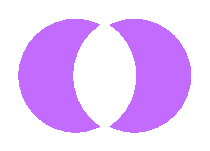
\includegraphics[height=3\baselineskip]{ABSOLUTEPATH/pictures/light-mode/symmetric-difference/definition/AsdiffB.pdf}}}%
                \hspace{0.5em}\scalebox{1.5}{$\mathbin{=}$}\hspace{0.5em}%
                \underset{\scalebox{1.25}{$\mkern7.0muU\setminus V$}}{\raisebox{-0.4\height}{
\includegraphics[height=3\baselineskip]{ABSOLUTEPATH/pictures/light-mode/symmetric-difference/definition/AsetminusB.pdf}}}%
                \hspace{0.5em}\scalebox{1.5}{$\mathbin{\cup}$}\hspace{0.5em}%
                \underset{\scalebox{1.25}{$\mkern7.0muV\setminus U$}}{\raisebox{-0.4\height}{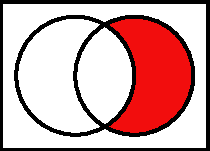
\includegraphics[height=3\baselineskip]{ABSOLUTEPATH/pictures/light-mode/symmetric-difference/definition/BsetminusA.pdf}}}%
                \mkern2.5mu.%
            $}%
        \end{webcompile}%%
        \par\vspace*{\TCBBoxCorrection}
    }%
    %---  End Footnote  ---%
    \[
        U\sdiff V
        \defeq
        (U\setminus V)%
        \cup%
        (V\setminus U).%
    \]%
\end{definition}
\begin{proposition}{Properties of Symmetric Differences}{properties-of-symmetric-differences}%
    Let $X$ be a set.
    \begin{enumerate}
        \item\label{properties-of-symmetric-differences-lack-of-functoriality}\SloganFont{Lack of Functoriality. }The assignment $(U,V)\mapsto U\sdiff V$ \demph{does not} in general define functors
            \[
                \BifunctorialityPeriod{U\sdiff-}{-\sdiff V}{-_{1}\sdiff-_{2}}{(\mathcal{P}(X),\subset)}{(\mathcal{P}(X),\subset)}{(\mathcal{P}(X)\times\mathcal{P}(X),\subset\times\subset)}{(\mathcal{P}(X),\subset)}%
            \]%
        \item\label{properties-of-symmetric-differences-via-unions-and-intersections}\SloganFont{Via Unions and Intersections. }We have%
            \[
                U\sdiff V%
                =%
                (U\cup V)\setminus(U\cap V)%
            \]%
            for each $U,V\in\mathcal{P}(X)$, as in the Venn diagram
            \begin{webcompile}
                \underset{\scalebox{1.0}{$\mkern3.5muU\sdiff V$}}{\raisebox{-0.4\height}{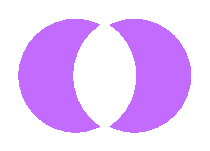
\includegraphics[height=2\baselineskip]{ABSOLUTEPATH/pictures/light-mode/symmetric-difference/via-unions-and-intersections/Venn0110.pdf}}}%
                \hspace{0.5em}\scalebox{1.5}{$\mathbin{=}$}\hspace{0.6em}%
                \underset{\scalebox{1.0}{$\mkern3.5muU\cup V$}}{\raisebox{-0.4\height}{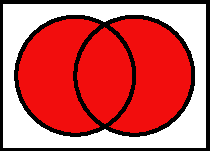
\includegraphics[height=2\baselineskip]{ABSOLUTEPATH/pictures/light-mode/symmetric-difference/via-unions-and-intersections/Venn0111.pdf}}}%
                \hspace{0.5em}\scalebox{1.5}{$\mathbin{\setminus}$}\hspace{0.5em}%
                \underset{\scalebox{1.0}{$\mkern3.5muU\cap V$}}{\raisebox{-0.4\height}{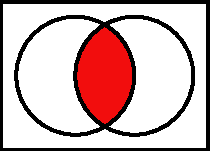
\includegraphics[height=2\baselineskip]{ABSOLUTEPATH/pictures/light-mode/symmetric-difference/via-unions-and-intersections/Venn0001.pdf}}}%
                \mkern2.5mu.%
            \end{webcompile}%%
        \item\label{properties-of-symmetric-differences-symmetric-differences-of-disjoint-sets}\SloganFont{Symmetric Differences of Disjoint Sets. }If $U$ and $V$ are disjoint, then we have
            \[
                U\sdiff V%
                =%
                U\cup V.%
            \]%
        \item\label{properties-of-symmetric-differences-associativity}\SloganFont{Associativity. }The diagram
            \[
                \begin{tikzcd}[row sep={0*\the\DL,between origins}, column sep={0*\the\DL,between origins}, background color=backgroundColor, ampersand replacement=\&]
                    \&[0.30901699437\TwoCmPlusHalf]
                    \&[0.5\TwoCmPlusHalf]
                    \mathcal{P}(X)\times(\mathcal{P}(X)\times\mathcal{P}(X))
                    \&[0.5\TwoCmPlusHalf]
                    \&[0.30901699437\TwoCmPlusHalf]
                    \\[0.58778525229\TwoCmPlusHalf]
                    (\mathcal{P}(X)\times\mathcal{P}(X))\times\mathcal{P}(X)
                    \&[0.30901699437\TwoCmPlusHalf]
                    \&[0.5\TwoCmPlusHalf]
                    \&[0.5\TwoCmPlusHalf]
                    \&[0.30901699437\TwoCmPlusHalf]
                    \mathcal{P}(X)\times\mathcal{P}(X)
                    \\[0.95105651629\TwoCmPlusHalf]
                    \&[0.30901699437\TwoCmPlusHalf]
                    \mathcal{P}(X)\times\mathcal{P}(X)
                    \&[0.5\TwoCmPlusHalf]
                    \&[0.5\TwoCmPlusHalf]
                    \mathcal{P}(X)\mrp{,}
                    \&[0.30901699437\TwoCmPlusHalf]
                    % 1-Arrows
                    % Left Boundary
                    \arrow[from=2-1,to=1-3,"\alpha^{\Sets}_{\mathcal{P}(X),\mathcal{P}(X),\mathcal{P}(X)}"{pos=0.35},isoarrowprime]%
                    \arrow[from=1-3,to=2-5,"{\id_{\mathcal{P}(X)}\times\mathord{\sdiff}}"{pos=0.55},""{name=2}]%
                    \arrow[from=2-5,to=3-4,"\sdiff"{pos=0.425}]%
                    % Right Boundary
                    \arrow[from=2-1,to=3-2,"{\mathord{\sdiff}\times\id_{\mathcal{P}(X)}}"'{pos=0.425}]%
                    \arrow[from=3-2,to=3-4,"\sdiff"']%
                \end{tikzcd}
            \]%
            commutes, i.e.\ we have%
            \[
                (U\sdiff V)\sdiff W
                =
                U\sdiff(V\sdiff W)
            \]%
            for each $U,V,W\in\mathcal{P}(X)$, as in the Venn diagram
            \begin{webcompile}
                \underset{\scalebox{1.0}{$\mkern3.75muU\sdiff V$}}{\raisebox{-0.4\height}{
\includegraphics[height=3\baselineskip]{ABSOLUTEPATH/pictures/light-mode/symmetric-difference/associativity/A_sdiff_B.pdf}}}%
                \hspace{0.5em}\scalebox{1.5}{$\mathbin{\sdiff}$}\hspace{0.5em}%
                \underset{\mcp{\scalebox{1.0}{$W$}}}{\raisebox{-0.4\height}{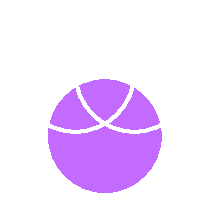
\includegraphics[height=3\baselineskip]{ABSOLUTEPATH/pictures/light-mode/symmetric-difference/associativity/C.pdf}}}%
                \hspace{0.5em}\scalebox{1.5}{$\mathbin{=}$}\hspace{0.3em}%
                \underset{\scalebox{1.0}{$U\sdiff V\sdiff W$}}{\raisebox{-0.4\height}{
\includegraphics[height=3\baselineskip]{ABSOLUTEPATH/pictures/light-mode/symmetric-difference/associativity/A_sdiff_B_sdiff_C.pdf}}}%
                \hspace{0.2em}\scalebox{1.5}{$\mathbin{=}$}\hspace{0.5em}%
                \underset{\mcp{\scalebox{1.0}{$U$}}}{\raisebox{-0.4\height}{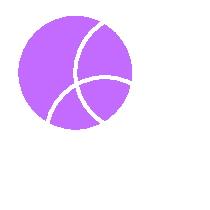
\includegraphics[height=3\baselineskip]{ABSOLUTEPATH/pictures/light-mode/symmetric-difference/associativity/A.pdf}}}%
                \hspace{0.5em}\scalebox{1.5}{$\mathbin{\sdiff}$}\hspace{0.5em}%
                \underset{\scalebox{1.0}{$\mkern4.25muV\sdiff W$}}{\raisebox{-0.4\height}{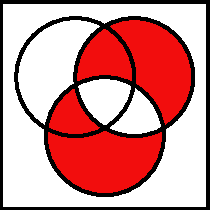
\includegraphics[height=3\baselineskip]{ABSOLUTEPATH/pictures/light-mode/symmetric-difference/associativity/B_sdiff_C.pdf}}}%
                \mkern2.5mu.%
            \end{webcompile}%%
        \item\label{properties-of-symmetric-differences-unitality}\SloganFont{Unitality. }The diagrams
            \begin{scalemath}
                \begin{tikzcd}[row sep={5.0*\the\DL,between origins}, column sep={11.25*\the\DL,between origins}, background color=backgroundColor, ampersand replacement=\&]
                    \pt\times\mathcal{P}(X)
                    \arrow[r,"{[\emptyset]\times\id_{\mathcal{P}(X)}}"]
                    \arrow[rd,"\LUnitor^{\Sets}_{\mathcal{P}(X)}"',isoarrow]
                    \&
                    \mathcal{P}(X)\times\mathcal{P}(X)
                    \arrow[d,"\sdiff"]
                    \\
                    \&
                    \mathcal{P}(X)
                \end{tikzcd}
                \quad
                \begin{tikzcd}[row sep={5.0*\the\DL,between origins}, column sep={11.25*\the\DL,between origins}, background color=backgroundColor, ampersand replacement=\&]
                    \mathcal{P}(X)\times\pt
                    \arrow[r,"{\id_{\mathcal{P}(X)}\times[\emptyset]}"]
                    \arrow[rd,"\RUnitor^{\Sets}_{\mathcal{P}(X)}"',isoarrow]
                    \&
                    \mathcal{P}(X)\times\mathcal{P}(X)
                    \arrow[d,"\sdiff"]
                    \\
                    \&
                    \mathcal{P}(X)
                \end{tikzcd}
            \end{scalemath}
            commute, i.e.\ we have
            \begin{align*}
                U\sdiff\emptyset  &= U,\\
                \emptyset\sdiff U &= U
            \end{align*}
            for each $U\in\mathcal{P}(X)$.
        \item\label{properties-of-symmetric-differences-commutativity}\SloganFont{Commutativity. }The diagram
            \[
                \begin{tikzcd}[row sep={5.0*\the\DL,between origins}, column sep={12.0*\the\DL,between origins}, background color=backgroundColor, ampersand replacement=\&]
                    \mathcal{P}(X)\times\mathcal{P}(X)
                    \arrow[r,"\sigma^{\Sets}_{\mathcal{P}(X),\mathcal{P}(X)}"]
                    \arrow[rd,"\sdiff"']
                    \&
                    \mathcal{P}(X)\times\mathcal{P}(X)
                    \arrow[d,"\sdiff"]
                    \\
                    \&
                    \mathcal{P}(X)
                \end{tikzcd}
            \]%
            commutes, i.e.\ we have
            \[
                U\sdiff V
                =
                V\sdiff U
            \]%
            for each $U,V\in\mathcal{P}(X)$.
        \item\label{properties-of-symmetric-differences-invertibility}\SloganFont{Invertibility. }We have
            \[
                U\sdiff U
                =
                \emptyset
            \]%
            for each $U\in\mathcal{P}(X)$.
        \item\label{properties-of-symmetric-differences-interaction-with-unions}\SloganFont{Interaction With Unions. }We have
            \[
                (U\sdiff V)\cup(V\sdiff T)
                =
                (U\cup V\cup W)\setminus(U\cap V\cap W)
            \]%
            for each $U,V,W\in\mathcal{P}(X)$.
        \item\label{properties-of-symmetric-differences-interaction-with-complements-1}\SloganFont{Interaction With Complements \rmI. }We have
            \[
                U\sdiff U^{\sfc}%
                =
                X%
            \]%
            for each $U\in\mathcal{P}(X)$.
        \item\label{properties-of-symmetric-differences-interaction-with-complements-2}\SloganFont{Interaction With Complements \rmII. }We have
            \begin{align*}
                U\sdiff X &= U^{\sfc},\\%
                X\sdiff U &= U^{\sfc}%
            \end{align*}
            for each $U\in\mathcal{P}(X)$.
        \item\label{properties-of-symmetric-differences-interaction-with-complements-3}\SloganFont{Interaction With Complements \rmIII. }The diagram
            \[
                \begin{tikzcd}[row sep={5.0*\the\DL,between origins}, column sep={8.0*\the\DL,between origins}, background color=backgroundColor, ampersand replacement=\&]
                    \mathcal{P}(X)\times\mathcal{P}(X)
                    \arrow[r,"\sdiff"]
                    \arrow[d,"{(-)^{\sfc}\times(-)^{\sfc}}"']
                    \&
                    \mathcal{P}(X)
                    \arrow[d,"{(-)^{\sfc}}"]
                    \\
                    \mathcal{P}(X)\times\mathcal{P}(X)
                    \arrow[r,"\sdiff"']
                    \&
                    \mathcal{P}(X)
                \end{tikzcd}
            \]%
            commutes, i.e.\ we have
            \[
                U^{\sfc}\sdiff V^{\sfc}%
                =%
                U\sdiff V%
            \]%
            for each $U,V\in\mathcal{P}(X)$.
        \item\label{properties-of-symmetric-differences-transitivity}\SloganFont{``Transitivity''. }We have
            \[
                (U\sdiff V)\sdiff(V\sdiff W)%
                =%
                U\sdiff W%
            \]%
            for each $U,V,W\in\mathcal{P}(X)$.
        \item\label{properties-of-symmetric-differences-the-triangle-inequality-for-symmetric-differences}\SloganFont{The Triangle Inequality for Symmetric Differences. }We have
            \[
                U\sdiff W%
                \subset%
                U\sdiff V%
                \cup
                V\sdiff W%
            \]%
            for each $U,V,W\in\mathcal{P}(X)$.
        \item\label{properties-of-symmetric-differences-distributivity-over-intersections}\SloganFont{Distributivity Over Intersections. }We have
            \begin{align*}
                U\cap(V\sdiff W)  &= (U\cap V)\sdiff(U\cap W),\\
                (U\sdiff V)\cap W &= (U\cap W)\sdiff(V\cap W)
            \end{align*}
            for each $U,V,W\in\mathcal{P}(X)$.
        \item\label{properties-of-symmetric-differences-interaction-with-characteristic-functions}\SloganFont{Interaction With Characteristic Functions. }We have
            \[
                \chi_{U\sdiff V}%
                =%
                \chi_{U}%
                +%
                \chi_{V}%
                -%
                2\chi_{U\cap V}%
            \]%
            and thus, in particular, we have
            \[
                \chi_{U\sdiff V}%
                \equiv%
                \chi_{U}+\chi_{V}%
                \mod{2}%
            \]%
            for each $U,V\in\mathcal{P}(X)$.
        \item\label{properties-of-symmetric-differences-bijectivity}\SloganFont{Bijectivity. }Given $U,V\in\mathcal{P}(X)$, the maps
            \begin{align*}
                U\sdiff-  &\colon \mathcal{P}(X) \to \mathcal{P}(X),\\
                -\sdiff V &\colon \mathcal{P}(X) \to \mathcal{P}(X)
            \end{align*}
            are bijections with inverses given by
            \begin{align*}
                (U\sdiff-)^{-1}  &= -\cup(U\cap-),\\
                (-\sdiff V)^{-1} &= -\cup(V\cap-).
            \end{align*}
            Moreover, the map
            \begin{webcompile}
                \begin{tikzcd}[row sep=0.0*\the\DL, column sep=1.0*\the\DL, background color=backgroundColor, ampersand replacement=\&]
                    \mathcal{P}(X)
                    \arrow[r]
                    \&
                    \mathcal{P}(X)
                    \\
                    C
                    \arrow[r, mapsto]
                    \&
                    C\sdiff(U\sdiff V)%
                \end{tikzcd}
            \end{webcompile}%
            is a bijection of $\mathcal{P}(X)$ onto itself sending $U$ to $V$ and $V$ to $U$.
        \item\label{properties-of-symmetric-differences-interaction-with-powersets-and-groups}\SloganFont{Interaction With Powersets and Groups. }Let $X$ be a set.
            \begin{enumerate}
                \item\label{properties-of-symmetric-differences-interaction-with-powersets-and-groups-a}The quadruple $(\mathcal{P}(X),\sdiff,\emptyset,\id_{\mathcal{P}(X)})$ is an abelian group.%
                    %--- Begin Footnote ---%
                    \footnote{%
                        Here are some examples:
                        \begin{enumerate}
                            \item When $X=\emptyset$, we have an isomorphism of groups between $\mathcal{P}(\emptyset)$ and the trivial group:
                                \[
                                    (\mathcal{P}(\emptyset),\sdiff,\emptyset,\id_{\mathcal{P}(\emptyset)})
                                    \cong
                                    \pt.
                                \]%
                            \item When $X=\pt$, we have an isomorphism of groups between $\mathcal{P}(\pt)$ and $\Zn{2}$:
                                \[
                                    (\mathcal{P}(\pt),\sdiff,\emptyset,\id_{\mathcal{P}(\pt)})
                                    \cong
                                    \Zn{2}.
                                \]%
                            \item When $X=\{0,1\}$, we have an isomorphism of groups between $\mathcal{P}(\{0,1\})$ and $\Zn{2}\times\Zn{2}$:
                                \[
                                    (\mathcal{P}(\{0,1\}),\sdiff,\emptyset,\id_{\mathcal{P}(\{0,1\})})
                                    \cong
                                    \Zn{2}\times\Zn{2}.
                                \]%
                        \end{enumerate}
                        \par\vspace*{\TCBBoxCorrection}
                    }%
                    %---  End Footnote  ---%
                \item\label{properties-of-symmetric-differences-interaction-with-powersets-and-groups-b}Every element of $\mathcal{P}(X)$ has order $2$ with respect to $\sdiff$, and thus $\mathcal{P}(X)$ is a \emph{Boolean group} (i.e.\ an abelian $2$-group).
            \end{enumerate}
        \item\label{properties-of-symmetric-differences-interaction-with-powersets-and-vector-spaces-1}\SloganFont{Interaction With Powersets and Vector Spaces \rmI. }The pair $(\mathcal{P}(X),\alpha_{\mathcal{P}(X)})$ consisting of
            \begin{itemize}
                \item The group $\mathcal{P}(X)$ of \cref{properties-of-symmetric-differences-interaction-with-powersets-and-groups};
                \item The map $\alpha_{\mathcal{P}(X)}\colon\F_{2}\times\mathcal{P}(X)\to\mathcal{P}(X)$ defined by
                    \begin{align*}
                        0\cdot U &\defeq \emptyset,\\
                        1\cdot U &\defeq U;
                    \end{align*}
            \end{itemize}
            is an $\F_{2}$-vector space.
        \item\label{properties-of-symmetric-differences-interaction-with-powersets-and-vector-spaces-2}\SloganFont{Interaction With Powersets and Vector Spaces \rmII. }If $X$ is finite, then:
            \begin{enumerate}% PROCESS %
                \item The set of singletons sets on the elements of $X$ forms a basis for the $\F_{2}$-vector space $(\mathcal{P}(X),\alpha_{\mathcal{P}(X)})$ of \cref{properties-of-symmetric-differences-interaction-with-powersets-and-vector-spaces-1}.
                \item We have
                    \[
                        \dim(\mathcal{P}(X))%
                        =%
                        \Card{X}.%
                    \]%
            \end{enumerate}% PROCESS %
        \item\label{properties-of-symmetric-differences-interaction-with-powersets-and-rings}\SloganFont{Interaction With Powersets and Rings. }The quintuple $(\mathcal{P}(X),\sdiff,\cap,\emptyset,X)$ is a commutative ring.%
            %--- Begin Footnote ---%
            \footnote{%
                \textdbend\SloganFont{Warning: }The analogous statement replacing intersections by unions (i.e.\ that the quintuple $(\mathcal{P}(X),\sdiff,\cup,\emptyset,X)$ is a ring) is false, however. See \cite{proof-wiki:symmetric-difference-with-union-does-not-form-ring} for a proof.

                END TEXTDBEND
                \par\vspace*{\TCBBoxCorrection}
            }%
            %---  End Footnote  ---%
        %\item\label{properties-of-symmetric-differences-}\SloganFont{. }
        \item\label{properties-of-symmetric-differences-interaction-with-direct-images}\SloganFont{Interaction With Direct Images. }We have a natural transformation
            \[
                \begin{tikzcd}[row sep={5.0*\the\DL,between origins}, column sep={11.5*\the\DL,between origins}, background color=backgroundColor, ampersand replacement=\&]
                    \mathcal{P}(X)^{\op}\times\mathcal{P}(X)
                    \arrow[r,"f^{\op}_{*}\times f_{*}"]
                    \arrow[d,"\sdiff"']
                    \&
                    \mathcal{P}(Y)^{\op}\times\mathcal{P}(Y)
                    \arrow[d,"\sdiff"]
                    \\
                    \mathcal{P}(X)
                    \arrow[r,"f_{*}"']
                    \&
                    \mathcal{P}(Y)
                    % 2-Arrows
                    \arrow[from=1-2,to=2-1,"\scalebox{1.5}{$\supset$}"{sloped,description},phantom,shorten <= 0.5*\the\DL,shorten >= 0.625*\the\DL,Rightarrow,pos=0.5]%
                \end{tikzcd}
            \]%
            with components
            \[
                f_{*}(U)\sdiff f_{*}(V)%
                \subset%
                f_{*}(U\sdiff V)%
            \]%
            indexed by $U,V\in\mathcal{P}(X)$.
        \item\label{properties-of-symmetric-differences-interaction-with-inverse-images}\SloganFont{Interaction With Inverse Images. }The diagram
            \[
                \begin{tikzcd}[row sep={5.0*\the\DL,between origins}, column sep={13.0*\the\DL,between origins}, background color=backgroundColor, ampersand replacement=\&]
                    \mathcal{P}(Y)^{\op}\times\mathcal{P}(Y)
                    \arrow[r,"f^{\op,-1}\times f^{-1}"]
                    \arrow[d,"\sdiff"']
                    \&
                    \mathcal{P}(X)^{\op}\times\mathcal{P}(X)
                    \arrow[d,"\sdiff"]
                    \\
                    \mathcal{P}(Y)
                    \arrow[r,"f^{-1}"']
                    \&
                    \mathcal{P}(X)
                \end{tikzcd}
            \]%
            i.e.\ we have
            \[
                f^{-1}(U)\sdiff f^{-1}(V)%
                =%
                f^{-1}(U\sdiff V)%
            \]%
            for each $U,V\in\mathcal{P}(Y)$.
        \item\label{properties-of-symmetric-differences-interaction-with-direct-images-with-compact-support}\SloganFont{Interaction With Direct Images With Compact Support. }We have a natural transformation
            \[
                \begin{tikzcd}[row sep={5.0*\the\DL,between origins}, column sep={11.5*\the\DL,between origins}, background color=backgroundColor, ampersand replacement=\&]
                    \mathcal{P}(X)^{\op}\times\mathcal{P}(X)
                    \arrow[r,"f^{\op}_{!}\times f_{!}"]
                    \arrow[d,"\sdiff"']
                    \&
                    \mathcal{P}(Y)^{\op}\times\mathcal{P}(Y)
                    \arrow[d,"\sdiff"]
                    \\
                    \mathcal{P}(X)
                    \arrow[r,"f_{!}"']
                    \&
                    \mathcal{P}(Y)
                    % 2-Arrows
                    \arrow[from=2-1,to=1-2,"\scalebox{1.5}{$\supset$}"{sloped,description},phantom,shorten <= 0.5*\the\DL,shorten >= 0.625*\the\DL,Rightarrow,pos=0.5]%
                \end{tikzcd}
            \]%
            with components
            \[
                f_{!}(U\sdiff V)%
                \subset%
                f_{1}(U)\sdiff f_{!}(V)%
            \]%
            indexed by $U,V\in\mathcal{P}(X)$.
    \end{enumerate}
\end{proposition}
\begin{Proof}{Proof of \cref{properties-of-symmetric-differences}}%
    \FirstProofBox{\cref{properties-of-symmetric-differences-lack-of-functoriality}: Lack of Functoriality}%
    Omitted.

    \ProofBox{\cref{properties-of-symmetric-differences-via-unions-and-intersections}: Via Unions and Intersections}%
    See \cite{proof-wiki:equivalence-of-definitions-of-symmetric-difference}.

    \ProofBox{\cref{properties-of-symmetric-differences-symmetric-differences-of-disjoint-sets}: Symmetric Differences of Disjoint Sets}%
    Since $U$ and $V$ are disjoint, we have $U\cap V=\emptyset$, and therefore we have
    \begin{align*}
        U\sdiff V &= (U\cup V)\setminus(U\cap V)\\
                  &= (U\cup V)\setminus\emptyset\\
                  &= U\cup V,
    \end{align*}
    where we've used \cref{properties-of-symmetric-differences-via-unions-and-intersections} and \cref{properties-of-differences-right-unitality} of \cref{properties-of-differences}.

    \ProofBox{\cref{properties-of-symmetric-differences-associativity}: Associativity}%
    See \cite{proof-wiki:symmetric-difference-is-associative}.

    \ProofBox{\cref{properties-of-symmetric-differences-unitality}: Unitality}%
    This follows from \cref{properties-of-symmetric-differences-commutativity} and \cite{proof-wiki:symmetric-difference-with-empty-set}.

    \ProofBox{\cref{properties-of-symmetric-differences-commutativity}: Commutativity}%
    See \cite{proof-wiki:symmetric-difference-is-commutative}.

    \ProofBox{\cref{properties-of-symmetric-differences-invertibility}: Invertibility}%
    See \cite{proof-wiki:symmetric-difference-with-self-is-empty-set}.

    \ProofBox{\cref{properties-of-symmetric-differences-interaction-with-unions}: Interaction With Unions}%
    See \cite{proof-wiki:union-of-symmetric-differences}.

    \ProofBox{\cref{properties-of-symmetric-differences-interaction-with-complements-1}: Interaction With Complements \rmI}%
    See \cite{proof-wiki:symmetric-difference-with-complement}.

    \ProofBox{\cref{properties-of-symmetric-differences-interaction-with-complements-2}: Interaction With Complements \rmII}%
    This follows from \cref{properties-of-symmetric-differences-commutativity} and \cite{proof-wiki:symmetric-difference-with-universe}.

    \ProofBox{\cref{properties-of-symmetric-differences-interaction-with-complements-3}: Interaction With Complements \rmIII}%
    See \cite{proof-wiki:symmetric-difference-of-complements}.

    \ProofBox{\cref{properties-of-symmetric-differences-transitivity}: ``Transitivity''}%
    We have
    % BEGIN RAW HTML %
    <div class="math-content">
        <div class="math-wrapper">
            <p>$(U\sdiff V)\sdiff(V\sdiff W) = \rlap{U\sdiff(V\sdiff(V\sdiff W))}\mkern{250mu}$</p>
            <p class="ptag">(by \cref{properties-of-symmetric-differences-associativity})</p>
        </div>
    </div>

    <div class="math-content">
        <div class="math-wrapper">
        <p>$\phantom{(U\sdiff V)\sdiff(V\sdiff W)} =\rlap{U\sdiff((V\sdiff V)\sdiff W)}\mkern{250mu}$</p>
            <p class="ptag">(by \cref{properties-of-symmetric-differences-associativity})</p>
        </div>
    </div>

    <div class="math-content">
        <div class="math-wrapper">
            <p>$\phantom{(U\sdiff V)\sdiff(V\sdiff W)} = \rlap{U\sdiff(\emptyset\sdiff W)}\mkern{250mu}$</p>
            <p class="ptag">(by \cref{properties-of-symmetric-differences-invertibility})</p>
        </div>
    </div>

    <div class="math-content">
        <div class="math-wrapper">
            <p>$\phantom{(U\sdiff V)\sdiff(V\sdiff W)} = \rlap{U\sdiff W}\mkern{250mu}$</p>
            <p class="ptag">(by \cref{properties-of-symmetric-differences-unitality})</p>
        </div>
    </div>
    % BEGIN LATEX HTML %
    \begin{align*}
        (U\sdiff V)\sdiff(V\sdiff W) &= U\sdiff(V\sdiff(V\sdiff W))  \ptag{by \cref{properties-of-symmetric-differences-associativity}}\\
                                     &= U\sdiff((V\sdiff V)\sdiff W) \ptag{by \cref{properties-of-symmetric-differences-associativity}}\\
                                     &= U\sdiff(\emptyset\sdiff W)   \ptag{by \cref{properties-of-symmetric-differences-invertibility}}\\
                                     &= U\sdiff W.                   \ptag{by \cref{properties-of-symmetric-differences-unitality}}
    \end{align*}
    % END RAW HTML %
    This finishes the proof.

    \ProofBox{\cref{properties-of-symmetric-differences-the-triangle-inequality-for-symmetric-differences}: The Triangle Inequality for Symmetric Differences}%
    This follows from \cref{properties-of-symmetric-differences-transitivity,properties-of-symmetric-differences-via-unions-and-intersections}.

    \ProofBox{\cref{properties-of-symmetric-differences-distributivity-over-intersections}: Distributivity Over Intersections}%
    See \cite{proof-wiki:intersection-distributes-over-symmetric-difference}.

    \ProofBox{\cref{properties-of-symmetric-differences-interaction-with-characteristic-functions}: Interaction With Characteristic Functions}%
    See \cite{proof-wiki:characteristic-function-of-symmetric-difference}.

    \ProofBox{\cref{properties-of-symmetric-differences-bijectivity}: Bijectivity}%
    Omitted.

    \ProofBox{\cref{properties-of-symmetric-differences-interaction-with-powersets-and-groups}: Interaction With Powersets and Groups}%
    \cref{properties-of-symmetric-differences-interaction-with-powersets-and-groups-a} follows from \cref{properties-of-symmetric-differences-associativity,properties-of-symmetric-differences-unitality,properties-of-symmetric-differences-invertibility,properties-of-symmetric-differences-commutativity}, while \cref{properties-of-symmetric-differences-interaction-with-powersets-and-groups-b} follows from \cref{properties-of-symmetric-differences-invertibility}.%
    %--- Begin Footnote ---%
    \footnote{%
        \SloganFont{Reference: }: \cite{proof-wiki:symmetric-difference-on-power-set-forms-abelian-group}.
    }%
    %---  End Footnote  ---%

    \ProofBox{\cref{properties-of-symmetric-differences-interaction-with-powersets-and-vector-spaces-1}: Interaction With Powersets and Vector Spaces \rmI}%
    See \cite{MSE2719059}.

    \ProofBox{\cref{properties-of-symmetric-differences-interaction-with-powersets-and-vector-spaces-2}: Interaction With Powersets and Vector Spaces \rmII}%
    See \cite{MSE2719059}.

    \ProofBox{\cref{properties-of-symmetric-differences-interaction-with-powersets-and-rings}: Interaction With Powersets and Rings}%
    This follows from \cref{properties-of-binary-intersections-annihilation-with-the-empty-set,properties-of-binary-intersections-interaction-with-powersets-and-monoids-with-zero} of \cref{properties-of-binary-intersections} and \cref{properties-of-symmetric-differences-distributivity-over-intersections,properties-of-symmetric-differences-interaction-with-powersets-and-groups}.%
    %--- Begin Footnote ---%
    \footnote{%
        \SloganFont{Reference: }\cite{proof-wiki:symmetric-difference-with-intersection-forms-ring}.
        \par\vspace*{\TCBBoxCorrection}
    }%
    %---  End Footnote  ---%

    \ProofBox{\cref{properties-of-symmetric-differences-interaction-with-direct-images}: Interaction With Direct Images}%
    This is a repetition of \cref{properties-of-direct-images-i-interaction-with-symmetric-differences} of \cref{properties-of-direct-images-i} and is proved there.

    \ProofBox{\cref{properties-of-symmetric-differences-interaction-with-inverse-images}: Interaction With Inverse Images}%
    This is a repetition of \cref{properties-of-inverse-images-i-interaction-with-symmetric-differences} of \cref{properties-of-inverse-images-i} and is proved there.

    \ProofBox{\cref{properties-of-symmetric-differences-interaction-with-direct-images-with-compact-support}: Interaction With Direct Images With Compact Support}%
    This is a repetition of \cref{properties-of-direct-images-with-compact-support-i-interaction-with-symmetric-differences} of \cref{properties-of-direct-images-with-compact-support-i} and is proved there.
\end{Proof}
\section{Powersets}\label{section-powersets}
\subsection{Foundations}\label{subsection-powersets-foundations}
Let $X$ be a set.%
\begin{definition}{Powersets}{powersets}%
    The \index[set-theory]{powerset}\textbf{powerset of $X$} is the set \index[notation]{PX@$\mathcal{P}(X)$}$\mathcal{P}(X)$ defined by
    \[
        \mathcal{P}(X)
        \defeq
        \{%
            U\in P%
            \ \middle|\ %
            U\subset X%
        \},
    \]%
    where $P$ is the set in the axiom of powerset, \cref{zermelo-fraenkel-set-theory-the-axiom-of-powerset} of \cref{zermelo-fraenkel-set-theory}.
\end{definition}
\begin{remark}{Powersets as Decategorifications of Co/Presheaf Categories}{powersets-as-decategorifications-of-co-presheaf-categories}%
    Under the analogy that $\TTV$ should be the $(-1)$-categorical analogue of $\Sets$, we may view the powerset of a set as a decategorification of the category of presheaves of a category (or of the category of copresheaves):%
    \begin{itemize}
        \item The powerset of a set $X$ is equivalently (\cref{properties-of-characteristic-functions-of-subsets-bijectivity} of \cref{properties-of-characteristic-functions-of-subsets}) the set
            \[%
                \Sets(X,\TTV)
            \]%
            of functions from $X$ to the set $\TTV$ of classical truth values.
        \item The category of presheaves on a category $\CatFont{C}$ is the category
            \[%
                \Fun(\CatFont{C}^{\op},\Sets)%
            \]%
            of functors from $\CatFont{C}^{\op}$ to the category $\Sets$ of sets.
    \end{itemize}
\end{remark}
\begin{notation}{Further Notation for Powersets}{further-notation-for-powersets}%
    Let $X$ be a set.
    \begin{enumerate}
        \item\label{further-notation-for-powersets-nonempty-powersets}We write \index[notation]{P0X@$\mathcal{P}_{0}(X)$}$\mathcal{P}_{0}(X)$ for the set of nonempty subsets of $X$.
        \item\label{further-notation-for-powersets-finite-powersets}We write \index[notation]{PfinX@$\mathcal{P}_{\fin}(X)$}$\mathcal{P}_{\fin}(X)$ for the set of finite subsets of $X$.
    \end{enumerate}
\end{notation}
\begin{proposition}{Elementary Properties of Powersets}{elementary-properties-of-powersets}%
    Let $X$ be a set.
    \begin{enumerate}
        \item\label{elementary-properties-of-powersets-co-completeness}\SloganFont{Co/Completeness. }The (posetal) category (associated to) $(\mathcal{P}(X),\subset)$ is complete and cocomplete:
            \begin{enumerate}
                \item\SloganFont{Products. }The products in $\mathcal{P}(X)$ are given by intersection of subsets.
                \item\SloganFont{Coproducts. }The coproducts in $\mathcal{P}(X)$ are given by union of subsets.
                \item\SloganFont{Co/Equalisers. }Being a posetal category, $\mathcal{P}(X)$ only has at most one morphisms between any two objects, so co/equalisers are trivial.
            \end{enumerate}
        \item\label{elementary-properties-of-powersets-cartesian-closedness}\SloganFont{Cartesian Closedness. }The category $\mathcal{P}(X)$ is Cartesian closed.
        \item\label{elementary-properties-of-powersets-powersets-as-sets-of-relations}\SloganFont{Powersets as Sets of Relations. }We have bijections
            \begin{align*}
                \mathcal{P}(X) &\cong \Rel(\pt,X),\\
                \mathcal{P}(X) &\cong \Rel(X,\pt),
            \end{align*}
            natural in $X\in\Obj(\Sets)$.
        \item\label{properties-of-powersets-as-categories-interaction-with-products-1}\SloganFont{Interaction With Products \rmI. }The map
            \begin{webcompile}
                \begin{tikzcd}[row sep=0.0*\the\DL, column sep=1.5*\the\DL, background color=backgroundColor, ampersand replacement=\&]
                    \mathcal{P}(X)\times\mathcal{P}(Y)%
                    \arrow[r]
                    \&
                    \mathcal{P}(X\icoprod Y)
                    \\
                    {(U,V)}
                    \arrow[r, mapsto]
                    \&
                    {U\cup V}
                \end{tikzcd}
            \end{webcompile}%
            is an isomorphism of sets, natural in $X,Y\in\Obj(\Sets)$ with respect to each of the functor structures $\mathcal{P}_{*}$, $\mathcal{P}^{-1}$, and $\mathcal{P}_{!}$ on $\mathcal{P}$ of \cref{functoriality-of-powersets}. Moreover, this makes $\mathcal{P}_{*}$, $\mathcal{P}^{-1}$, and $\mathcal{P}_{!}$ into symmetric monoidal functors.
        \item\label{properties-of-powersets-as-categories-interaction-with-products-2}\SloganFont{Interaction With Products \rmII. }The map
            \begin{webcompile}
                \begin{tikzcd}[row sep=0.0*\the\DL, column sep=1.5*\the\DL, background color=backgroundColor, ampersand replacement=\&]
                    \mathcal{P}(X)\times\mathcal{P}(Y)%
                    \arrow[r]
                    \&
                    \mathcal{P}(X\icoprod Y)
                    \\
                    {(U,V)}
                    \arrow[r, mapsto]
                    \&
                    {U\boxtimes_{X\times Y}V\mrp{,}}
                \end{tikzcd}
            \end{webcompile}%
            where\index[notation]{UboxtimesXYV@$U\boxtimes_{X\times Y}V$}%
            \[
                U\boxtimes_{X\times Y}V%
                \defeq%
                \{%
                    (u,v)\in X\times Y%
                    \ \middle|\ %
                    \text{$u\in U$ and $v\in V$}%
                \}%
            \]%
            is an inclusion of sets, natural in $X,Y\in\Obj(\Sets)$ with respect to each of the functor structures $\mathcal{P}_{*}$, $\mathcal{P}^{-1}$, and $\mathcal{P}_{!}$ on $\mathcal{P}$ of \cref{functoriality-of-powersets}. Moreover, this makes $\mathcal{P}_{*}$, $\mathcal{P}^{-1}$, and $\mathcal{P}_{!}$ into symmetric monoidal functors.
        \item\label{properties-of-powersets-as-categories-interaction-with-products-3}\SloganFont{Interaction With Products \rmIII. }We have an isomorphism
            \[
                \mathcal{P}(X)\otimes\mathcal{P}(Y)%
                \cong
                \mathcal{P}(X\times Y),%
            \]%
            natural in $X,Y\in\Obj(\Sets)$ with respect to each of the functor structures $\mathcal{P}_{*}$, $\mathcal{P}^{-1}$, and $\mathcal{P}_{!}$ on $\mathcal{P}$ of \cref{functoriality-of-powersets}, where $\otimes$ denotes the tensor product of suplattices of \cref{TODO}. Moreover, this makes $\mathcal{P}_{*}$, $\mathcal{P}^{-1}$, and $\mathcal{P}_{!}$ into symmetric monoidal functors.
        %\item\label{properties-of-powersets-as-categories-}\SloganFont{. }
    \end{enumerate}
\end{proposition}
\begin{Proof}{Proof of \cref{elementary-properties-of-powersets}}%
    \FirstProofBox{\cref{elementary-properties-of-powersets-co-completeness}: Co/Completeness}%
    Omitted.

    \ProofBox{\cref{elementary-properties-of-powersets-cartesian-closedness}: Cartesian Closedness}%
    See \cref{subsection-the-internal-hom-of-a-powerset}.

    \ProofBox{\cref{elementary-properties-of-powersets-powersets-as-sets-of-relations}: Powersets as Sets of Relations}%
    Indeed, we have
    \begin{align*}
        \Rel(\pt,X) &\defeq \mathcal{P}(\pt\times X)\\
                    &\cong  \mathcal{P}(X)
    \end{align*}
    and
    \begin{align*}
        \Rel(X,\pt) &\defeq \mathcal{P}(X\times\pt)\\
                    &\cong  \mathcal{P}(X),
    \end{align*}
    where we have used \cref{properties-of-products-of-sets-unitality} of  \cref{properties-of-products-of-sets}.

    \ProofBox{\cref{properties-of-powersets-as-categories-interaction-with-products-1}: Interaction With Products \rmI}%
    The inverse of the map in the statement is the map
    \[
        \Phi%
        \colon%
        \mathcal{P}(X\icoprod Y)%
        \to%
        \mathcal{P}(X)\times\mathcal{P}(Y)%
    \]%
    defined by
    \[
        \Phi(S)%
        \defeq%
        (S_{X},S_{Y})%
    \]%
    for each $S\in\mathcal{P}(X\icoprod Y)$, where
    \begin{align*}
        S_{X} &\defeq \{x\in X\ \middle|\ (0,x)\in S\}\\
        S_{Y} &\defeq \{y\in Y\ \middle|\ (1,y)\in S\}.
    \end{align*}
    The rest of the proof is omitted.

    \ProofBox{\cref{properties-of-powersets-as-categories-interaction-with-products-2}: Interaction With Products \rmII}%
    Omitted.

    \ProofBox{\cref{properties-of-powersets-as-categories-interaction-with-products-3}: Interaction With Products \rmIII}%
    Omitted.
\end{Proof}
\subsection{Functoriality of Powersets}\label{subsection-functoriality-of-powersets}
\begin{proposition}{Functoriality of Powersets}{functoriality-of-powersets}%
    Let $X$ be a set.
    \begin{enumerate}
        \item\label{functoriality-of-powersets-functoriality-1}\SloganFont{Functoriality \rmI. }The assignment $X\mapsto\mathcal{P}(X)$ defines a functor\index[notation]{Pstar@$\mathcal{P}_{*}$}
            \[
                \mathcal{P}_{*}%
                \colon%
                \Sets%
                \to%
                \Sets,%
            \]%
            where
            \begin{itemize}
                \item\SloganFont{Action on Objects. }For each $A\in\Obj(\Sets)$, we have
                    \[
                        \mathcal{P}_{*}(A)%
                        \defeq%
                        \mathcal{P}(A).%
                    \]%
                \item\SloganFont{Action on Morphisms. }For each $A,B\in\Obj(\Sets)$, the action on morphisms
                    \[
                        \mathcal{P}_{*|A,B}%
                        \colon%
                        \Sets(A,B)%
                        \to%
                        \Sets(\mathcal{P}(A),\mathcal{P}(B))%
                    \]%
                    of $\mathcal{P}_{*}$ at $(A,B)$ is the map defined by by sending a map of sets $f\colon A\to B$ to the map
                    \[
                        \mathcal{P}_{*}(f)%
                        \colon%
                        \mathcal{P}(A)%
                        \to%
                        \mathcal{P}(B)%
                    \]%
                    defined by
                    \[
                        \mathcal{P}_{*}(f)%
                        \defeq%
                        f_{*},%
                    \]%
                    as in \cref{the-direct-image-function-associated-to-a-function}.
            \end{itemize}
        \item\label{functoriality-of-powersets-functoriality-2}\SloganFont{Functoriality \rmII. }The assignment $X\mapsto\mathcal{P}(X)$ defines a functor\index[notation]{Pminusone@$\mathcal{P}^{-1}$}
            \[
                \mathcal{P}^{-1}%
                \colon%
                \Sets^{\op}%
                \to%
                \Sets,%
            \]%
            where
            \begin{itemize}
                \item\SloganFont{Action on Objects. }For each $A\in\Obj(\Sets)$, we have
                    \[
                        \mathcal{P}^{-1}(A)%
                        \defeq%
                        \mathcal{P}(A).%
                    \]%
                \item\SloganFont{Action on Morphisms. }For each $A,B\in\Obj(\Sets)$, the action on morphisms
                    \[
                        \mathcal{P}^{-1}_{A,B}%
                        \colon%
                        \Sets(A,B)%
                        \to%
                        \Sets(\mathcal{P}(B),\mathcal{P}(A))%
                    \]%
                    of $\mathcal{P}^{-1}$ at $(A,B)$ is the map defined by by sending a map of sets $f\colon A\to B$ to the map
                    \[
                        \mathcal{P}^{-1}(f)%
                        \colon%
                        \mathcal{P}(B)%
                        \to%
                        \mathcal{P}(A)%
                    \]%
                    defined by
                    \[
                        \mathcal{P}^{-1}(f)%
                        \defeq%
                        f^{-1},%
                    \]%
                    as in \cref{the-inverse-image-function-associated-to-a-function}.
            \end{itemize}
        \item\label{functoriality-of-powersets-functoriality-3}\SloganFont{Functoriality \rmIII. }The assignment $X\mapsto\mathcal{P}(X)$ defines a functor\index[notation]{Pshriek@$\mathcal{P}_{"!}$}
            \[
                \mathcal{P}_{!}%
                \colon%
                \Sets%
                \to%
                \Sets,%
            \]%
            where
            \begin{itemize}
                \item\SloganFont{Action on Objects. }For each $A\in\Obj(\Sets)$, we have
                    \[
                        \mathcal{P}_{!}(A)%
                        \defeq%
                        \mathcal{P}(A).%
                    \]%
                \item\SloganFont{Action on Morphisms. }For each $A,B\in\Obj(\Sets)$, the action on morphisms
                    \[
                        \mathcal{P}_{!|A,B}%
                        \colon%
                        \Sets(A,B)%
                        \to%
                        \Sets(\mathcal{P}(A),\mathcal{P}(B))%
                    \]%
                    of $\mathcal{P}_{!}$ at $(A,B)$ is the map defined by by sending a map of sets $f\colon A\to B$ to the map
                    \[
                        \mathcal{P}_{!}(f)%
                        \colon%
                        \mathcal{P}(A)%
                        \to%
                        \mathcal{P}(B)%
                    \]%
                    defined by
                    \[
                        \mathcal{P}_{!}(f)%
                        \defeq%
                        f_{!},%
                    \]%
                    as in \cref{the-direct-image-with-compact-support-function-associated-to-a-function}.
            \end{itemize}
    \end{enumerate}
\end{proposition}
\begin{Proof}{Proof of \cref{functoriality-of-powersets}}%
    \FirstProofBox{\cref{functoriality-of-powersets-functoriality-1}: Functoriality \rmI}%
    This follows from \cref{properties-of-direct-images-ii-interaction-with-identities,properties-of-direct-images-ii-interaction-with-composition} of \cref{properties-of-direct-images-ii}.

    \ProofBox{\cref{functoriality-of-powersets-functoriality-2}: Functoriality \rmII}%
    This follows from \cref{properties-of-inverse-images-ii-interaction-with-identities,properties-of-inverse-images-ii-interaction-with-composition} of \cref{properties-of-inverse-images-ii}.

    \ProofBox{\cref{functoriality-of-powersets-functoriality-3}: Functoriality \rmIII}%
    This follows from \cref{properties-of-direct-images-with-compact-support-ii-interaction-with-identities,properties-of-direct-images-with-compact-support-ii-interaction-with-composition} of \cref{properties-of-direct-images-with-compact-support-ii}.
\end{Proof}
\subsection{Adjointness of Powersets \rmI}\label{subsection-adjointness-of-powersets-1}
\begin{proposition}{Adjointness of Powersets \rmI}{adjointness-of-powersets-1}%
    We have an adjunction
    \begin{webcompile}
        \Adjunction#\mathcal{P}^{-1}#\mathcal{P}^{-1,\op}#\Sets^{\op}#\Sets,#
    \end{webcompile}%
    witnessed by a bijection
    \[
        \underbrace{\Sets^{\op}(\mathcal{P}(X),Y)}_{\defeq\mkern5mu\Sets(Y,\mathcal{P}(X))}
        \cong
        \Sets(X,\mathcal{P}(Y)),
    \]%
    natural in $X\in\Obj(\Sets)$ and $Y\in\Obj(\Sets^{\op})$.
\end{proposition}
\begin{Proof}{Proof of \cref{adjointness-of-powersets-1}}%
    We have
    % BEGIN RAW HTML %
    <hr style="margin-top: 0.0em; visibility: hidden;">
    <div class="math-content">
        <div class="math-wrapper">
            <p>$\Sets^{\op}(\mathcal{P}(A),B) \defeq \rlap{\Sets(B,\mathcal{P}(A))}\phantom{\mkern400mu}$</p>
            <p class="ptag"></p>
        </div>
    </div>
    <div class="math-content">
        <div class="math-wrapper">
        <p>$\phantom{\Sets^{\op}(\mathcal{P}(X),Y)}\cong\rlap{\Sets(B,\Sets(A,\TTV))}\phantom{\mkern400mu}$</p>
            <p class="ptag">(by \cref{properties-of-characteristic-functions-of-subsets-bijectivity} of \cref{properties-of-characteristic-functions-of-subsets})</p>
        </div>
    </div>
    <div class="math-content">
        <div class="math-wrapper">
            <p>$\phantom{\Sets^{\op}(\mathcal{P}(X),Y)} \cong \rlap{\Sets(A\times B,\TTV)}\phantom{\mkern400mu}$</p>
            <p class="ptag">(by \cref{properties-of-products-of-sets-adjointness} of \cref{properties-of-products-of-sets})</p>
        </div>
    </div>
    <div class="math-content">
        <div class="math-wrapper">
            <p>$\phantom{\Sets^{\op}(\mathcal{P}(X),Y)} \cong \rlap{\Sets(A,\Sets(B,\TTV))}\phantom{\mkern400mu}$</p>
            <p class="ptag">(by \cref{properties-of-products-of-sets-adjointness} of \cref{properties-of-products-of-sets})</p>
        </div>
    </div>
    <div class="math-content">
        <div class="math-wrapper">
            <p>$\phantom{\Sets^{\op}(\mathcal{P}(X),Y)} \cong \rlap{\Sets(A,\mathcal{P}(B))}\phantom{\mkern400mu}$</p>
            <p class="ptag">(by \cref{properties-of-characteristic-functions-of-subsets-bijectivity} of \cref{properties-of-characteristic-functions-of-subsets})</p>
        </div>
    </div>
    <hr style="margin-top: 0.0em; visibility: hidden;">
    % BEGIN LATEX HTML %
    \begin{align*}
        \Sets^{\op}(\mathcal{P}(A),B) &\defeq \Sets(B,\mathcal{P}(A))\\
                                      &\cong  \Sets(B,\Sets(A,\TTV))  \ptag{by \cref{properties-of-characteristic-functions-of-subsets-bijectivity} of \cref{properties-of-characteristic-functions-of-subsets}}\\
                                      &\cong  \Sets(A\times B,\TTV)   \ptag{by \cref{properties-of-products-of-sets-adjointness} of \cref{properties-of-products-of-sets}}\\
                                      &\cong  \Sets(A,\Sets(B,\TTV))  \ptag{by \cref{properties-of-products-of-sets-adjointness} of \cref{properties-of-products-of-sets}}\\
                                      &\cong  \Sets(A,\mathcal{P}(B)) \ptag{by \cref{properties-of-characteristic-functions-of-subsets-bijectivity} of \cref{properties-of-characteristic-functions-of-subsets}}
    \end{align*}
    % END RAW HTML %
    with all bijections natural in $A$ and $B$.%
    %--- Begin Footnote ---%
    \footnote{%
        Here we are using \cref{properties-of-characteristic-functions-of-subsets-naturality} of \cref{properties-of-characteristic-functions-of-subsets}.
        \par\vspace*{\TCBBoxCorrection}
    }%
    %---  End Footnote  ---%
\end{Proof}
\subsection{Adjointness of Powersets \rmII}\label{subsection-adjointness-of-powersets-2}
\begin{proposition}{Adjointness of Powersets \rmII}{adjointness-of-powersets-2}%
    We have an adjunction
    \begin{webcompile}
        \Adjunction#\Gr#\mathcal{P}_{*}#\Sets#\Rel,#
    \end{webcompile}%
    witnessed by a bijection of sets%
    \[
        \Rel(\Gr(X),Y)
        \cong
        \Sets(X,\mathcal{P}(Y))
    \]%
    natural in $X\in\Obj(\Sets)$ and $Y\in\Obj(\Rel)$, where $\Gr$ is the graph functor of \ChapterRef{\ChapterConstructionsWithRelations, \cref{constructions-with-relations:properties-of-graphs-of-functions-functoriality} of \cref{constructions-with-relations:properties-of-graphs-of-functions}}{\cref{properties-of-graphs-of-functions-functoriality} of \cref{properties-of-graphs-of-functions}} and $\mathcal{P}_{*}$ is the functor of \ChapterRef{\ChapterConstructionsWithRelations, \cref{constructions-with-relations:functoriality-of-powersets-1}}{\cref{functoriality-of-powersets-1}}.
\end{proposition}
\begin{Proof}{Proof of \cref{adjointness-of-powersets-2}}%
    We have
    % BEGIN RAW HTML %
    <hr style="margin-top: 0.0em; visibility: hidden;">
    <div class="math-content">
        <div class="math-wrapper">
            <p>$\Rel(\Gr(A),B) \defeq \rlap{\mathcal{P}(A\times B)}\phantom{\mkern375mu}$</p>
            <p class="ptag"></p>
        </div>
    </div>

    <div class="math-content">
        <div class="math-wrapper">
        <p>$\phantom{\Rel(\Gr(A),B)} \cong\rlap{\Sets(A\times B,\TTV)}\phantom{\mkern375mu}$</p>
            <p class="ptag">(by \cref{properties-of-characteristic-functions-of-subsets-bijectivity} of \cref{properties-of-characteristic-functions-of-subsets})</p>
        </div>
    </div>

    <div class="math-content">
        <div class="math-wrapper">
            <p>$\phantom{\Rel(\Gr(A),B)} \cong \rlap{\Sets(A,\Sets(B,\TTV))}\phantom{\mkern375mu}$</p>
            <p class="ptag">(by \cref{properties-of-products-of-sets-adjointness} of \cref{properties-of-products-of-sets})</p>
        </div>
    </div>

    <div class="math-content">
        <div class="math-wrapper">
            <p>$\phantom{\Rel(\Gr(A),B)} \cong \rlap{\Sets(A,\mathcal{P}(B))}\phantom{\mkern375mu}$</p>
            <p class="ptag">(by \cref{properties-of-characteristic-functions-of-subsets-bijectivity} of \cref{properties-of-characteristic-functions-of-subsets})</p>
        </div>
    </div>
    <hr style="margin-top: 0.0em; visibility: hidden;">
    % BEGIN LATEX HTML %
    \begin{align*}
        \Rel(\Gr(A),B) &\cong \mathcal{P}(A\times B)\\
                       &\cong \Sets(A\times B,\TTV)   \ptag{by \cref{properties-of-characteristic-functions-of-subsets-bijectivity} of \cref{properties-of-characteristic-functions-of-subsets}}\\
                       &\cong \Sets(A,\Sets(B,\TTV))  \ptag{by \cref{properties-of-products-of-sets-adjointness} of \cref{properties-of-products-of-sets}}\\
                       &\cong \Sets(A,\mathcal{P}(B)) \ptag{by \cref{properties-of-characteristic-functions-of-subsets-bijectivity} of \cref{properties-of-characteristic-functions-of-subsets}}
    \end{align*}
    % END RAW HTML %
    with all bijections natural in $A$, (where we are using \cref{properties-of-characteristic-functions-of-subsets-naturality} of \cref{properties-of-characteristic-functions-of-subsets}). Explicitly, this isomorphism is given by sending a relation $R\colon\Gr(A)\rightproarrow B$ to the map $R^{\dagger}\colon A\to\mathcal{P}(B)$ sending $a$ to the subset $R(a)$ of $B$, as in \ChapterRef{\ChapterRelations, \cref{relations:relations}}{\cref{relations}}.
    % BEGIN RAW HTML %
    <hr style="margin-top: 0.0em; visibility: hidden;">
    % BEGIN LATEX HTML %

    \vspace{0.5\baselineskip}
    % END RAW HTML %
    Naturality in $B$ is then the statement that given a relation $R\colon B\rightproarrow B'$, the diagram
    \[
        \begin{tikzcd}[row sep={5.0*\the\DL,between origins}, column sep={9.0*\the\DL,between origins}, background color=backgroundColor, ampersand replacement=\&]
            \Rel(\Gr(A),B)
            \arrow[r,"{R\procirc-}"]
            \arrow[d,isoarrowprime]
            \&
            \Rel(\Gr(A),B')
            \arrow[d,isoarrow]
            \\
            \Sets(A,\mathcal{P}(B))
            \arrow[r,"R_{*}"']
            \&
            \Sets(A,\mathcal{P}(B'))
        \end{tikzcd}
    \]%
    commutes, which follows from \ChapterRef{\ChapterConstructionsWithRelations, \cref{constructions-with-relations:unwinding-the-direct-image-function-associated-to-a-relation}}{\cref{unwinding-the-direct-image-function-associated-to-a-relation}}.
\end{Proof}
\subsection{Powersets as Free Cocompletions}\label{subsection-powersets-as-free-cocompletions}
Let $X$ be a set.
\begin{proposition}{Powersets as Free Cocompletions: Universal Property}{powersets-as-free-cocompletions-universal-property}%
    The pair $(\mathcal{P}(X),\chi_{(-)})$ consisting of
    \begin{itemize}
        \item The powerset $(\mathcal{P}(X),\subset)$ of $X$ of \cref{powersets};
        \item The characteristic embedding $\chi_{(-)}\colon X\hookrightarrow\mathcal{P}(X)$ of $X$ into $\mathcal{P}(X)$ of \cref{the-characteristic-embedding-of-a-set};
    \end{itemize}
    satisfies the following universal property:

    \begin{itemize}
        \item[$(\star)$]Given another pair $(Y,f)$ consisting of
            \begin{itemize}
                \item A suplattice $(Y,\preceq)$;
                \item A function $f\colon X\to Y$;
            \end{itemize}
            there exists a unique morphism of suplattices
            \[
                (\mathcal{P}(X),\subset)\uearrow(Y,\preceq)%
            \]%
            making the diagram
            \[
                \begin{tikzcd}[row sep={5.0*\the\DL,between origins}, column sep={5.0*\the\DL,between origins}, background color=backgroundColor, ampersand replacement=\&]
                    \&
                    \mathcal{P}(X)
                    \arrow[d,"\exists!",dashed]
                    \\
                    X
                    \arrow[r,"f"']
                    \arrow[ru,"{\chi_{X}}"]
                    \&
                    Y
                \end{tikzcd}
            \]%
            commute.
    \end{itemize}
\end{proposition}
\begin{Proof}{Proof of \cref{powersets-as-free-cocompletions-universal-property}}%
    This is a rephrasing of \cref{powersets-as-free-cocompletions-adjointness}, which we prove below.%
    %--- Begin Footnote ---%
    \footnote{%
        Here we only remark that the unique morphism of suplattices in the statement is given by the left Kan extension $\Lan_{\chi_{X}}(f)$ of $f$ along $\chi_{X}$.
        \par\vspace*{\TCBBoxCorrection}
    }%
    %---  End Footnote  ---%
\end{Proof}
\begin{proposition}{Powersets as Free Cocompletions: Adjointness}{powersets-as-free-cocompletions-adjointness}%
    We have an adjunction%
    \begin{webcompile}
        \Adjunction#\mathcal{P}#\Wasureru#\Sets#\SupLat,#
    \end{webcompile}%
    witnessed by a bijection%
    \[
        \SupLat((\mathcal{P}(X),\subset),(Y,\preceq))
        \cong%
        \Sets(X,Y),
    \]%
    natural in $X\in\Obj(\Sets)$ and $(Y,\preceq)\in\Obj(\SupLat)$, where:
    \begin{itemize}
        \item The category $\SupLat$ is the category of suplattices of \cref{TODO}.
        \item The map
            \[
                \chi^{*}_{X}
                \colon
                \SupLat((\mathcal{P}(X),\subset),(Y,\preceq))
                \to
                \Sets(X,Y)
            \]%
            witnessing the above bijection is defined by
            \[
                \chi^{*}_{X}(f)
                \defeq
                f\circ\chi_{X},
            \]%
            i.e.\ by sending a morphism of suplattices $f\colon\mathcal{P}(X)\to Y$ to the composition
            \[
                X
                \xlonghookrightarrow{\chi_{X}}
                \mathcal{P}(X)
                \xlongrightarrow{f}
                Y.
            \]%
        \item The map
            \[
                \Lan_{\chi_{X}}
                \colon
                \Sets(X,Y)
                \to
                \SupLat((\mathcal{P}(X),\subset),(Y,\preceq))
            \]%
            witnessing the above bijection is given by sending a function $f\colon X\to Y$ to its left Kan extension along $\chi_{X}$,
            \begin{webcompile}
                \Lan_{\chi_{X}}(f)\colon\mathcal{P}(X)\to Y,%
                \quad%
                \begin{tikzcd}[row sep={5.0*\the\DL,between origins}, column sep={5.0*\the\DL,between origins}, background color=backgroundColor, ampersand replacement=\&]
                    \&
                    \mathcal{P}(X)
                    \arrow[d, "{\Lan_{\chi_{X}}(f)}",dashed]
                    \\
                    X
                    \arrow[ru, "\chi_{X}"]
                    \arrow[r,"f"'{name=F}]
                    \&
                    Y\mrp{.}%
                    % 2-Arrows
                    \arrow[from=F,to=1-2,Rightarrow,shorten=0.5em,pos=0.5]
                \end{tikzcd}
            \end{webcompile}
            Moreover, invoking the bijection $\mathcal{P}(X)\cong\Sets(X,\TTV)$ of \cref{properties-of-characteristic-functions-of-subsets-bijectivity} of \cref{properties-of-characteristic-functions-of-subsets}, $\Lan_{\chi_{X}}(f)$ can be explicitly computed by
            \begin{align*}
                [\Lan_{\chi_{X}}(f)](U) &= \int^{x\in X}\chi_{\mathcal{P}(X)}(\chi_{x},U)\odot f(x)\\
                                        &= \int^{x\in X}\chi_{U}(x)\odot f(x)\\
                                        &= \bigvee_{x\in X}(\chi_{U}(x)\odot f(x))\\
                                        &= \left(\bigvee_{x\in U}(\chi_{U}(x)\odot f(x))\right)\vee\left(\bigvee_{x\in U^{\sfc}}(\chi_{U}(x)\odot f(x))\right)\\
                                        &= \left(\bigvee_{x\in U}f(x)\right)\vee\left(\bigvee_{x\in U^{\sfc}}\BottomElement_{Y}\right)\\
                                        &= \bigvee_{x\in U}f(x)
            \end{align*}
            for each $U\in\mathcal{P}(X)$, where:
            \begin{itemize}
                \item We have used \cref{TODO} for the first equality.
                \item We have used \cref{the-yoneda-lemma-for-sets} for the second equality.
                \item We have used \cref{TODO} for the third equality.
                \item The symbol $\bigvee$ denotes the join in $(Y,\preceq)$.
                \item The symbol $\odot$ denotes the tensor of an element of $Y$ by a truth value as in \cref{TODO}. In particular, we have
                    \begin{align*}
                        \true\odot f(x)  &\defeq f(x),\\
                        \false\odot f(x) &\defeq \BottomElement_{Y},
                    \end{align*}
                    where $\BottomElement_{Y}$ is the bottom element of $(Y,\preceq)$.
            \end{itemize}
            In particular, when $(Y,\preceq_{Y})=(\mathcal{P}(B),\subset)$ for some set $B$, the Kan extension $\Lan_{\chi_{X}}(f)$ is given by
            \begin{align*}
                [\Lan_{\chi_{X}}(f)](U) &= \bigvee_{x\in U}f(x)\\
                                        &= \bigcup_{x\in U}f(x)
            \end{align*}
            for each $U\in\mathcal{P}(X)$.
    \end{itemize}
\end{proposition}
\begin{Proof}{Proof of \cref{powersets-as-free-cocompletions-adjointness}}%
    \ProofBox{Map \rmI}%
    We define a map
    \[
        \Phi_{X,Y}%
        \colon%
        \SupLat((\mathcal{P}(X),\subset),(Y,\preceq))
        \to%
        \Sets(X,Y)
    \]%
    as in the statement, i.e.\ by
    \[
        \Phi_{X,Y}(f)%
        \defeq%
        f\circ\chi_{X}%
    \]%
    for each $f\in\SupLat((\mathcal{P}(X),\subset),(Y,\preceq))$.

    \ProofBox{Map \rmII}%
    We define a map
    \[
        \Psi_{X,Y}%
        \colon%
        \Sets(X,Y)%
        \to%
        \SupLat((\mathcal{P}(X),\subset),(Y,\preceq))%
    \]%
    as in the statement, i.e.\ by
    \begin{webcompile}
        \Psi_{X,Y}(f)%
        \defeq%
        \Lan_{\chi_{X}}(f),%
        \quad%
        \begin{tikzcd}[row sep={5.0*\the\DL,between origins}, column sep={5.0*\the\DL,between origins}, background color=backgroundColor, ampersand replacement=\&]
            \&
            \mathcal{P}(X)
            \arrow[d, "{\Lan_{\chi_{X}}(f)}",dashed]
            \arrow[d, phantom]
            \\
            X
            \arrow[ru, "\chi_{X}"]
            \arrow[r,"f"'{name=F}]
            \&
            Y\mrp{,}%
            % 2-Arrows
            \arrow[from=F,to=1-2,Rightarrow,shorten=0.5em,pos=0.5]
        \end{tikzcd}
    \end{webcompile}
    for each $f\in\Sets(X,Y)$.

    \ProofBox{Invertibility \rmI}%
    We claim that
    \[
        \Psi_{X,Y}\circ\Phi_{X,Y}%
        =%
        \id_{\SupLat((\mathcal{P}(X),\subset),(Y,\preceq))}.%
    \]%
    We have
    \begin{align*}
        [\Psi_{X,Y}\circ\Phi_{X,Y}](f) &\defeq \Psi_{X,Y}(\Phi_{X,Y}(f))\\%
                                       &\defeq \Psi_{X,Y}(f\circ\chi_{X})\\%
                                       &\defeq \Lan_{\chi_{X}}(f\circ\chi_{X})\\%
    \end{align*}
    for each $f\in\SupLat((\mathcal{P}(X),\subset),(Y,\preceq))$. We now claim that
    \[
        \Lan_{\chi_{X}}(f\circ\chi_{X})%
        =%
        f%
    \]%
    for each $f\in\SupLat((\mathcal{P}(X),\subset),(Y,\preceq))$. Indeed, we have
    \begin{align*}
        \left[\Lan_{\chi_{X}}(f\circ\chi_{X})\right](U) &= \bigvee_{x\in U} f(\chi_{X}(x))\\%
                                                        &= f\left(\bigvee_{x\in U}\chi_{X}(x)\right)\\%
                                                        &= f\left(\bigcup_{x\in U}\{x\}\right)\\%
                                                        &= f(U)%
    \end{align*}
    for each $U\in\mathcal{P}(X)$, where we have used that $f$ is a morphism of suplattices and hence preserves joins for the second equality. This proves our claim. Since we have shown that
    \[
        [\Psi_{X,Y}\circ\Phi_{X,Y}](f)%
        =%
        f%
    \]%
    for each $f\in\SupLat((\mathcal{P}(X),\subset),(Y,\preceq))$, it follows that $\Psi_{X,Y}\circ\Phi_{X,Y}$ must be equal to the identity map $\id_{\SupLat((\mathcal{P}(X),\subset),(Y,\preceq))}$ of $\SupLat((\mathcal{P}(X),\subset),(Y,\preceq))$.

    \ProofBox{Invertibility \rmII}%
    We claim that
    \[
        \Phi_{X,Y}\circ\Psi_{X,Y}%
        =%
        \id_{\Sets(X,Y)}.%
    \]%
    We have
    \begin{align*}
        [\Phi_{X,Y}\circ\Psi_{X,Y}](f) &\defeq  \Phi_{X,Y}(\Psi_{X,Y}(f))\\%
                                       &\defeq  \Phi_{X,Y}(\Lan_{\chi_{X}}(f))\\%
                                       &\defeq  \Lan_{\chi_{X}}(f)\circ\chi_{X}%
    \end{align*}
    for each $f\in\Sets(X,Y)$. We now claim that
    \[
        \Lan_{\chi_{X}}(f)\circ\chi_{X}%
        =%
        f%
    \]%
    for each $f\in\Sets(X,Y)$. Indeed, we have
    \begin{align*}
        [\Lan_{\chi_{X}}(f)\circ\chi_{X}](x) &= \bigvee_{y\in\{x\}}f(y)\\%
                                             &= f(x)%
    \end{align*}
    for each $x\in X$. This proves our claim. Since we have shown that
    \[
        [\Phi_{X,Y}\circ\Psi_{X,Y}](f)%
        =%
        f%
    \]%
    for each $f\in\Sets(X,Y)$, it follows that $\Phi_{X,Y}\circ\Psi_{X,Y}$ must be equal to the identity map $\id_{\Sets(X,Y)}$ of $\Sets(X,Y)$.

    \ProofBox{Naturality for $\Phi$, Part \rmI}%
    We need to show that, given a function $f\colon X\to X'$, the diagram
    \[
        \begin{tikzcd}[row sep={5.0*\the\DL,between origins}, column sep={12.25*\the\DL,between origins}, background color=backgroundColor, ampersand replacement=\&]
            \SupLat((\mathcal{P}(X'),\subset),(Y,\preceq))%
            \arrow[r,"\Phi_{X',Y}"]
            \arrow[d,"{\mathcal{P}_{*}(f)}^{*}"']
            \&
            \Sets(X',Y)
            \arrow[d,"f^{*}"]
            \\
            \SupLat((\mathcal{P}(X),\subset),(Y,\preceq))%
            \arrow[r,"\Phi_{X,Y}"']
            \&
            \Sets(X,Y)
        \end{tikzcd}
    \]%
    commutes. Indeed, we have
    \begin{align*}
        [\Phi_{X,Y}\circ\mathcal{P}_{*}(f)^{*}](\xi) &\defeq  \Phi_{X,Y}(\mathcal{P}_{*}(f)^{*}(\xi))\\
                                                     &\defeq  \Phi_{X,Y}(\xi\circ f_{*})\\
                                                     &\defeq  (\xi\circ f_{*})\circ\chi_{X}\\
                                                     &=       \xi\circ(f_{*}\circ\chi_{X})\\
                                                     &\eqstar \xi\circ(\chi_{X'}\circ f)\\
                                                     &=       (\xi\circ\chi_{X'})\circ f\\
                                                     &\defeq  \Phi_{X',Y}(\xi)\circ f\\
                                                     &\defeq  f^{*}(\Phi_{X',Y}(\xi))\\
                                                     &\defeq  [f^{*}\circ\Phi_{X',Y}](\xi),
    \end{align*}
    for each $\xi\in\SupLat((\mathcal{P}(X'),\subset),(Y,\preceq))$, where we have used \cref{properties-of-characteristic-embeddings-interaction-with-functions} of \cref{properties-of-characteristic-embeddings} for the fifth equality above.

    \ProofBox{Naturality for $\Phi$, Part \rmII}%
    We need to show that, given a morphism of suplattices
    \[
        g%
        \colon%
        (Y,\preceq_{Y})%
        \to%
        (Y',\preceq_{Y'}),%
    \]%
    the diagram
    \[
        \begin{tikzcd}[row sep={5.0*\the\DL,between origins}, column sep={12.5*\the\DL,between origins}, background color=backgroundColor, ampersand replacement=\&]
            \SupLat((\mathcal{P}(X),\subset),(Y,\preceq))%
            \arrow[r,"\Phi_{X,Y}"]
            \arrow[d,"g_{*}"']
            \&
            \Sets(X,Y)
            \arrow[d,"g_{*}"]
            \\
            \SupLat((\mathcal{P}(X),\subset),(Y',\preceq))%
            \arrow[r,"\Phi_{X,Y'}"']
            \&
            \Sets(X,Y')
        \end{tikzcd}
    \]%
    commutes. Indeed, we have
    \begin{align*}
        [\Phi_{X,Y'}\circ g_{*}](\xi) &\defeq \Phi_{X,Y'}(g_{*}(\xi))\\
                                      &\defeq \Phi_{X,Y'}(g\circ\xi)\\
                                      &\defeq (g\circ\xi)\circ\chi_{X}\\
                                      &=      g\circ(\xi\circ\chi_{X})\\
                                      &\defeq g\circ(\Phi_{X,Y}(\xi))\\
                                      &\defeq g_{*}(\Phi_{X,Y}(\xi))\\
                                      &\defeq [g_{*}\circ\Phi_{X,Y}](\xi).
    \end{align*}
    for each $\xi\in\SupLat((\mathcal{P}(X),\subset),(Y,\preceq))$.

    \ProofBox{Naturality for $\Psi$}%
    Since $\Phi$ is natural in each argument and $\Phi$ is a componentwise inverse to $\Psi$ in each argument, it follows from \ChapterRef{\ChapterCategories, \cref{categories:properties-of-natural-isomorphisms-componentwise-inverses-of-natural-transformations-assemble-into-natural-transformations} of \cref{categories:properties-of-natural-isomorphisms}}{\cref{properties-of-natural-isomorphisms-componentwise-inverses-of-natural-transformations-assemble-into-natural-transformations} of \cref{properties-of-natural-isomorphisms}} that $\Psi$ is also natural in each argument.
\end{Proof}
\begin{warning}{Free Cocompletion Is Not an Idempotent Operation}{free-cocompletion-is-not-an-idempotent-operation}
    Although the assignment $X\mapsto\mathcal{P}(X)$ is called the \textit{free cocompletion of $X$}, it is not an idempotent operation, i.e.\ we have $\mathcal{P}(\mathcal{P}(X))\neq\mathcal{P}(X)$.
\end{warning}
\subsection{Powersets as Free Completions}\label{subsection-powersets-as-free-completions}
Let $X$ be a set.
\begin{proposition}{Powersets as Free Completions: Universal Property}{powersets-as-free-completions-universal-property}%
    The pair $(\mathcal{P}(X),\chi_{(-)})$ consisting of
    \begin{itemize}
        \item The powerset of $X$ together with reverse inclusion $\mathcal{P}(X)^{\op}=(\mathcal{P}(X),\supset)$ of \cref{powersets};
        \item The characteristic embedding $\chi_{(-)}\colon X\hookrightarrow\mathcal{P}(X)$ of $X$ into $\mathcal{P}(X)$ of \cref{the-characteristic-embedding-of-a-set};
    \end{itemize}
    satisfies the following universal property:

    \begin{itemize}
        \item[$(\star)$]Given another pair $(Y,f)$ consisting of
            \begin{itemize}
                \item An inflattice $(Y,\preceq)$;
                \item A function $f\colon X\to Y$;
            \end{itemize}
            there exists a unique morphism of inflattices
            \[
                (\mathcal{P}(X),\supset)\uearrow(Y,\preceq)%
            \]%
            making the diagram
            \[
                \begin{tikzcd}[row sep={5.0*\the\DL,between origins}, column sep={5.0*\the\DL,between origins}, background color=backgroundColor, ampersand replacement=\&]
                    \&
                    \mathcal{P}(X)^{\op}
                    \arrow[d,"\exists!",dashed]
                    \\
                    X
                    \arrow[r,"f"']
                    \arrow[ru,"{\chi_{X}}"]
                    \&
                    Y
                \end{tikzcd}
            \]%
            commute.
    \end{itemize}
\end{proposition}
\begin{Proof}{Proof of \cref{powersets-as-free-completions-universal-property}}%
    This is a rephrasing of \cref{powersets-as-free-completions-adjointness}, which we prove below.%
    %--- Begin Footnote ---%
    \footnote{%
        Here we only remark that the unique morphism of inflattices in the statement is given by the right Kan extension $\Ran_{\chi_{X}}(f)$ of $f$ along $\chi_{X}$.
        \par\vspace*{\TCBBoxCorrection}
    }%
    %---  End Footnote  ---%
\end{Proof}
\begin{proposition}{Powersets as Free Completions: Adjointness}{powersets-as-free-completions-adjointness}%
    We have an adjunction%
    \begin{webcompile}
        \Adjunction#\mathcal{P}#\Wasureru#\Sets#\InfLat,#
    \end{webcompile}%
    witnessed by a bijection%
    \[
        \InfLat((\mathcal{P}(X),\supset),(Y,\preceq))
        \cong%
        \Sets(X,Y),
    \]%
    natural in $X\in\Obj(\Sets)$ and $(Y,\preceq)\in\Obj(\InfLat)$, where:
    \begin{itemize}
        \item The category $\InfLat$ is the category of inflattices of \cref{TODO}.
        \item The map
            \[
                \chi^{*}_{X}
                \colon
                \InfLat((\mathcal{P}(X),\supset),(Y,\preceq))
                \to
                \Sets(X,Y)
            \]%
            witnessing the above bijection is defined by
            \[
                \chi^{*}_{X}(f)
                \defeq
                f\circ\chi_{X},
            \]%
            i.e.\ by sending a morphism of inflattices $f\colon\mathcal{P}(X)^{\op}\to Y$ to the composition
            \[
                X
                \xlonghookrightarrow{\chi_{X}}
                \mathcal{P}(X)^{\op}
                \xlongrightarrow{f}
                Y.
            \]%
        \item The map
            \[
                \Ran_{\chi_{X}}
                \colon
                \Sets(X,Y)
                \to
                \InfLat((\mathcal{P}(X),\supset),(Y,\preceq))
            \]%
            witnessing the above bijection is given by sending a function $f\colon X\to Y$ to its right Kan extension along $\chi_{X}$,
            \begin{webcompile}
                \Ran_{\chi_{X}}(f)\colon\mathcal{P}(X)^{\op}\to Y,%
                \quad%
                \begin{tikzcd}[row sep={5.0*\the\DL,between origins}, column sep={5.0*\the\DL,between origins}, background color=backgroundColor, ampersand replacement=\&]
                    \&
                    \mathcal{P}(X)^{\op}
                    \arrow[d, "{\Ran_{\chi_{X}}(f)}",dashed]
                    \\
                    X
                    \arrow[ru, "\chi_{X}"]
                    \arrow[r,"f"'{name=F}]
                    \&
                    Y\mrp{.}%
                    % 2-Arrows
                    \arrow[from=1-2,to=F,Rightarrow,shorten=0.5em,pos=0.5]
                \end{tikzcd}
            \end{webcompile}
            Moreover, invoking the bijection $\mathcal{P}(X)\cong\Sets(X,\TTV)$ of \cref{properties-of-characteristic-functions-of-subsets-bijectivity} of \cref{properties-of-characteristic-functions-of-subsets}, $\Ran_{\chi_{X}}(f)$ can be explicitly computed by
            \begin{align*}
                [\Ran_{\chi_{X}}(f)](U) &= \int_{x\in X}\chi_{\mathcal{P}(X)^{\op}}(\chi_{x},U)\pitchfork f(x)\\
                                        &= \int_{x\in X}\chi_{\mathcal{P}(X)}(U,\chi_{x})\pitchfork f(x)\\
                                        &= \int_{x\in X}\chi_{U}(x)\pitchfork f(x)\\
                                        &= \bigwedge_{x\in X}\chi_{U}(x)\pitchfork f(x)\\
                                        &= \left(\bigwedge_{x\in U}\chi_{U}(x)\pitchfork f(x)\right)\wedge\left(\bigwedge_{x\in U^{\sfc}}\chi_{U}(x)\pitchfork f(x)\right)\\
                                        &= \left(\bigwedge_{x\in U}f(x)\right)\wedge\left(\bigwedge_{x\in U^{\sfc}}\TopElement_{Y}\right)\\
                                        &= \left(\bigwedge_{x\in U}f(x)\right)\wedge\TopElement_{Y}\\
                                        &= \bigwedge_{x\in U}f(x)
            \end{align*}
            for each $U\in\mathcal{P}(X)$, where:
            \begin{itemize}
                \item We have used \cref{TODO} for the first equality.
                \item We have used \cref{the-yoneda-lemma-for-sets} for the second equality.
                \item We have used \cref{TODO} for the third equality.
                \item The symbol $\bigwedge$ denotes the meet in $(Y,\preceq)$.
                \item The symbol $\pitchfork$ denotes the cotensor of an element of $Y$ by a truth value as in \cref{TODO}. In particular, we have
                    \begin{align*}
                        \true\pitchfork f(x)  &\defeq f(x),\\
                        \false\pitchfork f(x) &\defeq \TopElement_{Y},
                    \end{align*}
                    where $\TopElement_{Y}$ is the top element of $(Y,\preceq)$.
            \end{itemize}
            In particular, when $(Y,\preceq_{Y})=(\mathcal{P}(B),\subset)$ for some set $B$, the Kan extension $\Ran_{\chi_{X}}(f)$ is given by
            \begin{align*}
                [\Ran_{\chi_{X}}(f)](U) &= \bigwedge_{x\in U}f(x)\\
                                        &= \bigcap_{x\in U}f(x)
            \end{align*}
            for each $U\in\mathcal{P}(X)$.
    \end{itemize}
\end{proposition}
\begin{Proof}{Proof of \cref{powersets-as-free-cocompletions-adjointness}}%
    \ProofBox{Map \rmI}%
    We define a map
    \[
        \Phi_{X,Y}%
        \colon%
        \InfLat((\mathcal{P}(X),\supset),(Y,\preceq))
        \to%
        \Sets(X,Y)
    \]%
    as in the statement, i.e.\ by
    \[
        \Phi_{X,Y}(f)%
        \defeq%
        f\circ\chi_{X}%
    \]%
    for each $f\in\InfLat((\mathcal{P}(X),\supset),(Y,\preceq))$.

    \ProofBox{Map \rmII}%
    We define a map
    \[
        \Psi_{X,Y}%
        \colon%
        \Sets(X,Y)%
        \to%
        \InfLat((\mathcal{P}(X),\supset),(Y,\preceq))%
    \]%
    as in the statement, i.e.\ by
    \begin{webcompile}
        \Psi_{X,Y}(f)%
        \defeq%
        \Ran_{\chi_{X}}(f),%
        \quad%
        \begin{tikzcd}[row sep={5.0*\the\DL,between origins}, column sep={5.0*\the\DL,between origins}, background color=backgroundColor, ampersand replacement=\&]
            \&
            \mathcal{P}(X)
            \arrow[d, "{\Ran_{\chi_{X}}(f)}",dashed]
            \arrow[d, phantom]
            \\
            X
            \arrow[ru, "\chi_{X}"]
            \arrow[r,"f"'{name=F}]
            \&
            Y\mrp{,}%
            % 2-Arrows
            \arrow[from=1-2,to=F,Rightarrow,shorten=0.5em,pos=0.5]
        \end{tikzcd}
    \end{webcompile}
    for each $f\in\Sets(X,Y)$.

    \ProofBox{Invertibility \rmI}%
    We claim that
    \[
        \Psi_{X,Y}\circ\Phi_{X,Y}%
        =%
        \id_{\InfLat((\mathcal{P}(X),\supset),(Y,\preceq))}.%
    \]%
    We have
    \begin{align*}
        [\Psi_{X,Y}\circ\Phi_{X,Y}](f) &\defeq \Psi_{X,Y}(\Phi_{X,Y}(f))\\%
                                       &\defeq \Psi_{X,Y}(f\circ\chi_{X})\\%
                                       &\defeq \Ran_{\chi_{X}}(f\circ\chi_{X})\\%
    \end{align*}
    for each $f\in\InfLat((\mathcal{P}(X),\supset),(Y,\preceq))$. We now claim that
    \[
        \Ran_{\chi_{X}}(f\circ\chi_{X})%
        =%
        f%
    \]%
    for each $f\in\InfLat((\mathcal{P}(X),\supset),(Y,\preceq))$. Indeed, we have
    \begin{align*}
        \left[\Ran_{\chi_{X}}(f\circ\chi_{X})\right](U) &= \bigwedge_{x\in U}f(\chi_{X}(x))\\%
                                                        &= f\left(\bigwedge_{x\in U}\chi_{X}(x)\right)\\%
                                                        &= f\left(\bigcup_{x\in U}\{x\}\right)\\%
                                                        &= f(U)%
    \end{align*}
    for each $U\in\mathcal{P}(X)$, where we have used that $f$ is a morphism of inflattices and hence preserves meets in $(\mathcal{P}(X),\supset)$ (i.e.\ joins in $(\mathcal{P}(X),\subset)$) for the second equality. This proves our claim. Since we have shown that
    \[
        [\Psi_{X,Y}\circ\Phi_{X,Y}](f)%
        =%
        f%
    \]%
    for each $f\in\InfLat((\mathcal{P}(X),\supset),(Y,\preceq))$, it follows that $\Psi_{X,Y}\circ\Phi_{X,Y}$ must be equal to the identity map $\id_{\InfLat((\mathcal{P}(X),\supset),(Y,\preceq))}$ of $\InfLat((\mathcal{P}(X),\supset),(Y,\preceq))$.

    \ProofBox{Invertibility \rmII}%
    We claim that
    \[
        \Phi_{X,Y}\circ\Psi_{X,Y}%
        =%
        \id_{\Sets(X,Y)}.%
    \]%
    We have
    \begin{align*}
        [\Phi_{X,Y}\circ\Psi_{X,Y}](f) &\defeq  \Phi_{X,Y}(\Psi_{X,Y}(f))\\%
                                       &\defeq  \Phi_{X,Y}(\Ran_{\chi_{X}}(f))\\%
                                       &\defeq  \Ran_{\chi_{X}}(f)\circ\chi_{X}%
    \end{align*}
    for each $f\in\Sets(X,Y)$. We now claim that
    \[
        \Ran_{\chi_{X}}(f)\circ\chi_{X}%
        =%
        f%
    \]%
    for each $f\in\Sets(X,Y)$. Indeed, we have
    \begin{align*}
        [\Ran_{\chi_{X}}(f)\circ\chi_{X}](x) &= \bigwedge_{y\in\{x\}}f(y)\\%
                                             &= f(x)%
    \end{align*}
    for each $x\in X$. This proves our claim. Since we have shown that
    \[
        [\Phi_{X,Y}\circ\Psi_{X,Y}](f)%
        =%
        f%
    \]%
    for each $f\in\Sets(X,Y)$, it follows that $\Phi_{X,Y}\circ\Psi_{X,Y}$ must be equal to the identity map $\id_{\Sets(X,Y)}$ of $\Sets(X,Y)$.

    \ProofBox{Naturality for $\Phi$, Part \rmI}%
    We need to show that, given a function $f\colon X\to X'$, the diagram
    \[
        \begin{tikzcd}[row sep={5.0*\the\DL,between origins}, column sep={12.25*\the\DL,between origins}, background color=backgroundColor, ampersand replacement=\&]
            \InfLat((\mathcal{P}(X'),\supset),(Y,\preceq))%
            \arrow[r,"\Phi_{X',Y}"]
            \arrow[d,"{\mathcal{P}_{*}(f)}^{*}"']
            \&
            \Sets(X',Y)
            \arrow[d,"f^{*}"]
            \\
            \InfLat((\mathcal{P}(X),\supset),(Y,\preceq))%
            \arrow[r,"\Phi_{X,Y}"']
            \&
            \Sets(X,Y)
        \end{tikzcd}
    \]%
    commutes. Indeed, we have
    \begin{align*}
        [\Phi_{X,Y}\circ\mathcal{P}_{*}(f)^{*}](\xi) &\defeq  \Phi_{X,Y}(\mathcal{P}_{*}(f)^{*}(\xi))\\
                                                     &\defeq  \Phi_{X,Y}(\xi\circ f_{*})\\
                                                     &\defeq  (\xi\circ f_{*})\circ\chi_{X}\\
                                                     &=       \xi\circ(f_{*}\circ\chi_{X})\\
                                                     &\eqstar \xi\circ(\chi_{X'}\circ f)\\
                                                     &=       (\xi\circ\chi_{X'})\circ f\\
                                                     &\defeq  \Phi_{X',Y}(\xi)\circ f\\
                                                     &\defeq  f^{*}(\Phi_{X',Y}(\xi))\\
                                                     &\defeq  [f^{*}\circ\Phi_{X',Y}](\xi),
    \end{align*}
    for each $\xi\in\InfLat((\mathcal{P}(X'),\supset),(Y,\preceq))$, where we have used \cref{properties-of-characteristic-embeddings-interaction-with-functions} of \cref{properties-of-characteristic-embeddings} for the fifth equality above.

    \ProofBox{Naturality for $\Phi$, Part \rmII}%
    We need to show that, given a cocontinuous morphism of posets
    \[
        g%
        \colon%
        (Y,\preceq_{Y})%
        \to%
        (Y',\preceq_{Y'}),%
    \]%
    the diagram
    \[
        \begin{tikzcd}[row sep={5.0*\the\DL,between origins}, column sep={12.25*\the\DL,between origins}, background color=backgroundColor, ampersand replacement=\&]
            \InfLat((\mathcal{P}(X),\supset),(Y,\preceq))%
            \arrow[r,"\Phi_{X,Y}"]
            \arrow[d,"g_{*}"']
            \&
            \Sets(X,Y)
            \arrow[d,"g_{*}"]
            \\
            \InfLat((\mathcal{P}(X),\supset),(Y',\preceq))%
            \arrow[r,"\Phi_{X,Y'}"']
            \&
            \Sets(X,Y')
        \end{tikzcd}
    \]%
    commutes. Indeed, we have
    \begin{align*}
        [\Phi_{X,Y'}\circ g_{*}](\xi) &\defeq \Phi_{X,Y'}(g_{*}(\xi))\\
                                      &\defeq \Phi_{X,Y'}(g\circ\xi)\\
                                      &\defeq (g\circ\xi)\circ\chi_{X}\\
                                      &=      g\circ(\xi\circ\chi_{X})\\
                                      &\defeq g\circ(\Phi_{X,Y}(\xi))\\
                                      &\defeq g_{*}(\Phi_{X,Y}(\xi))\\
                                      &\defeq [g_{*}\circ\Phi_{X,Y}](\xi).
    \end{align*}
    for each $\xi\in\InfLat((\mathcal{P}(X),\supset),(Y,\preceq))$.

    \ProofBox{Naturality for $\Psi$}%
    Since $\Phi$ is natural in each argument and $\Phi$ is a componentwise inverse to $\Psi$ in each argument, it follows from \ChapterRef{\ChapterCategories, \cref{categories:properties-of-natural-isomorphisms-componentwise-inverses-of-natural-transformations-assemble-into-natural-transformations} of \cref{categories:properties-of-natural-isomorphisms}}{\cref{properties-of-natural-isomorphisms-componentwise-inverses-of-natural-transformations-assemble-into-natural-transformations} of \cref{properties-of-natural-isomorphisms}} that $\Psi$ is also natural in each argument.
\end{Proof}
\begin{warning}{Free Completion Is Not an Idempotent Operation}{free-completion-is-not-an-idempotent-operation}
    Although the assignment $X\mapsto\mathcal{P}(X)^{\op}$ is called the \textit{free completion of $X$}, it is not an idempotent operation, i.e.\ we have $\mathcal{P}(\mathcal{P}(X)^{\op})^{\op}\neq\mathcal{P}(X)^{\op}$.
\end{warning}
\subsection{The Internal Hom of a Powerset}\label{subsection-the-internal-hom-of-a-powerset}
Let $X$ be a set and let $U,V\in\mathcal{P}(X)$.
\begin{definition}{The Internal Hom of a Powerset}{the-internal-hom-of-a-powerset}%
    The \index[set-theory]{powerset!internal Hom of@internal Hom of}\textbf{internal Hom of $\mathcal{P}(X)$ from $U$ to $V$} is the subset \index[notation]{UVX@$[U,V]_{X}$}$[U,V]_{X}$%
    %--- Begin Footnote ---%
    \footnote{%
        \SloganFont{Further Notation: }Also written \index[notation]{HomPXUV@$\eHom_{\mathcal{P}(X)}(U,V)$}$\eHom_{\mathcal{P}(X)}(U,V)$.
        \par\vspace*{\TCBBoxCorrection}
    } %
    %---  End Footnote  ---%
    of $X$ defined by
    \begin{align*}
        [U,V]_{X} &\defeq U^{\sfc}\cup V\\%
                  &=      (U\setminus V)^{\sfc}%
    \end{align*}
    where $U^{\sfc}$ is the complement of $U$ of \cref{complements}.
\end{definition}
\begin{Proof}{Proof of \cref{the-internal-hom-of-a-powerset}}%
    We have
    \begin{align*}
        (U\setminus V)^{\sfc} &\defeq X\setminus(U\setminus V)\\%
                              &=      (X\cap V)\cup(X\setminus U)\\%
                              &=      V\cup(X\setminus U)\\%
                              &\defeq V\cup U^{\sfc}\\%
                              &=      U^{\sfc}\cup V,%
    \end{align*}
    where we have used:
    \begin{enumerate}
        \item \cref{properties-of-differences-triple-differences} of \cref{properties-of-differences} for the second equality.
        \item \cref{properties-of-binary-intersections-unitality} of \cref{properties-of-binary-intersections} for the third equality.
        \item \cref{properties-of-binary-unions-commutativity} of \cref{properties-of-binary-unions} for the last equality.
    \end{enumerate}
    This finishes the proof.
\end{Proof}
\begin{remark}{Intuition for the Internal Hom of $\mathcal{P}(X)$}{intuition-for-the-internal-hom-of-px}%
    Henning Makholm suggests the following heuristic intuition for the internal Hom of $\mathcal{P}(X)$ from $U$ to $V$ (\cite{MSE267365}):
    \begin{enumerate}
        \item\label{intuition-for-the-internal-hom-of-px-1}Since products in $\mathcal{P}(X)$ are given by binary intersections (\cref{elementary-properties-of-powersets-co-completeness} of \cref{elementary-properties-of-powersets}), the right adjoint $\eHom_{\mathcal{P}(X)}(U,-)$ of $U\cap-$ may be thought of as a function type $[U,V]$.
        \item\label{intuition-for-the-internal-hom-of-px-2}Under the Curry--Howard correspondence (\cref{TODO}), the function type $[U,V]$ corresponds to implication $U\Longrightarrow V$.
        \item\label{intuition-for-the-internal-hom-of-px-3}Implication $U\Rightarrow V$ is logically equivalent to $\neg U\vee V$.
        \item\label{intuition-for-the-internal-hom-of-px-4}The expression $\neg U\vee V$ then corresponds to the set $U^{\sfc}\cup V$ in $\mathcal{P}(X)$.
        \item\label{intuition-for-the-internal-hom-of-px-5}The set $U^{\sfc}\vee V$ turns out to indeed be the internal Hom of $\mathcal{P}(X)$.
    \end{enumerate}
\end{remark}
\begin{proposition}{Properties of Internal Homs of Powersets}{properties-of-internal-homs-of-powersets}%
    Let $X$ be a set.
    \begin{enumerate}
        \item\label{properties-of-internal-homs-of-powersets-functoriality}\SloganFont{Functoriality. }The assignments $U,V,(U,V)\mapsto\eHom_{\mathcal{P}(X)}$ define functors
            \[
                \BifunctorialityPeriod{{[U,-]_{X}}}{{[-,V]_{X}}}{{[-_{1},-_{2}]_{X}}}{{(\mathcal{P}(X),\supset)}}{{(\mathcal{P}(X),\subset)}}{{(\mathcal{P}(X)\times\mathcal{P}(X),\subset\times\supset)}}{{(\mathcal{P}(X),\subset)}}%
            \]%
            In particular, the following statements hold for each $U,V,A,B\in\mathcal{P}(X)$:
            \begin{enumerate}
                \item\label{properties-of-internal-homs-of-powersets-functoriality-1}If $U\subset A$, then $[A,V]_{X}\subset[U,V]_{X}$.
                \item\label{properties-of-internal-homs-of-powersets-functoriality-2}If $V\subset B$, then $[U,V]_{X}\subset[U,B]_{X}$.
                \item\label{properties-of-internal-homs-of-powersets-functoriality-3}If $U\subset A$ and $V\subset B$, then $[A,V]_{X}\subset[U,B]_{X}$.
            \end{enumerate}
        \item\label{properties-of-internal-homs-of-powersets-adjointness}\SloganFont{Adjointness. }We have adjunctions
            \begin{webcompile}
                \begin{gathered}
                    \Adjunction#U\cap -#{[U,-]_{X}}#\mathcal{P}(X)#\mathcal{P}(X),#\\
                    \Adjunction#-\cap V#{[V,-]_{X}}#\mathcal{P}(X)#\mathcal{P}(X),#
                \end{gathered}
            \end{webcompile}%
            witnessed by bijections
            \begin{align*}
                \Hom_{\mathcal{P}(X)}(U\cap V,W) &\cong \Hom_{\mathcal{P}(X)}(U,[V,W]_{X}),\\
                \Hom_{\mathcal{P}(X)}(U\cap V,W) &\cong \Hom_{\mathcal{P}(X)}(V,[U,W]_{X}).
            \end{align*}
            In particular, the following statements hold for each $U,V,W\in\mathcal{P}(X)$:
            \begin{enumerate}
                \item\label{properties-of-internal-homs-of-powersets-adjointness-adjointness-a}The following conditions are equivalent:
                    \begin{enumerate}
                        \item\label{properties-of-internal-homs-of-powersets-adjointness-adjointness-a-i}We have $U\cap V\subset W$.
                        \item\label{properties-of-internal-homs-of-powersets-adjointness-adjointness-a-ii}We have $U\subset[V,W]_{X}$.
                    \end{enumerate}
                \item\label{properties-of-internal-homs-of-powersets-adjointness-adjointness-b}The following conditions are equivalent:
                    \begin{enumerate}
                        \item\label{properties-of-internal-homs-of-powersets-adjointness-adjointness-b-i}We have $U\cap V\subset W$.
                        \item\label{properties-of-internal-homs-of-powersets-adjointness-adjointness-b-ii}We have $V\subset[U,W]_{X}$.
                    \end{enumerate}
            \end{enumerate}
        \item\label{properties-of-internal-homs-of-powersets-interaction-with-the-empty-set-1}\SloganFont{Interaction With the Empty Set \rmI. }We have
            \begin{align*}
                [U,\emptyset]_{X} &= U^{\sfc},\\
                [\emptyset,V]_{X} &= X,
            \end{align*}
            natural in $U,V\in\mathcal{P}(X)$.
        \item\label{properties-of-internal-homs-of-powersets-interaction-with-x}\SloganFont{Interaction With $X$. }We have
            \begin{align*}
                [U,X]_{X} &= X,\\
                [X,V]_{X} &= V,
            \end{align*}
            natural in $U,V\in\mathcal{P}(X)$.
        \item\label{properties-of-internal-homs-of-powersets-interaction-with-the-empty-set-2}\SloganFont{Interaction With the Empty Set \rmII. }The functor
            \[
                D_{X}
                \colon%
                \mathcal{P}(X)^{\op}%
                \to
                \mathcal{P}(X)%
            \]%
            defined by
            \begin{align*}
                D_{X} &\defeq [-,\emptyset]_{X}\\%
                      &=      (-)^{\sfc}%
            \end{align*}
            is an involutory isomorphism of categories, making $\emptyset$ into a dualising object for $(\mathcal{P}(X),\cap,X,[-,-]_{X})$ in the sense of \cref{TODO}. In particular:
            \begin{enumerate}
                \item\label{properties-of-internal-homs-of-powersets-interaction-with-the-empty-set-2-a}The diagram
                    \[
                        \begin{tikzcd}[row sep={5.0*\the\DL,between origins}, column sep={6.0*\the\DL,between origins}, background color=backgroundColor, ampersand replacement=\&]
                            {\mathcal{P}(X)^{\op}}
                            \arrow[r,"D_{X}"]
                            \arrow[rd,"\id_{\mathcal{P}(X)^{\op}}"']
                            \&
                            {\mathcal{P}(X)}%
                            \arrow[d,"D_{X}"]
                            \\
                            \&
                            {\mathcal{P}(X)^{\op}}
                        \end{tikzcd}
                    \]%
                    commutes, i.e.\ we have
                    \[
                        \underbrace{D_{X}(D_{X}(U))}_{\defeq[[U,\emptyset]_{X},\emptyset]_{X}}%
                        =%
                        U%
                    \]%
                    for each $U\in\mathcal{P}(X)$.
                \item\label{properties-of-internal-homs-of-powersets-interaction-with-the-empty-set-2-b}The diagram
                    \[
                        \begin{tikzcd}[row sep={0.0*\the\DL,between origins}, column sep={0.0*\the\DL,between origins}, background color=backgroundColor, ampersand replacement=\&]
                            \&[0.5\ThreeCmPlusAQuarter]
                            {\mathcal{P}(X)^{\op}\times\mathcal{P}(X)^{\op}}
                            \&[0.9\ThreeCmPlusAQuarter]
                            \mathcal{P}(X)^{\op}
                            \&[0.5\ThreeCmPlusAQuarter]
                            \\[0.5\ThreeCmPlusAQuarter]
                            {\mathcal{P}(X)^{\op}\times\mathcal{P}(X)}
                            \&[0.5\ThreeCmPlusAQuarter]
                            \&[0.9\ThreeCmPlusAQuarter]
                            \&[0.5\ThreeCmPlusAQuarter]
                            {\mathcal{P}(X)}
                            % 1-Arrows
                            \arrow[from=2-1,to=1-2,"\id_{\mathcal{P}(X)^{\op}}\times D_{X}",pos=0.325]%
                            \arrow[from=1-2,to=1-3,"\cap^{\op}"]%
                            \arrow[from=1-3,to=2-4,"D_{X}",pos=0.525]%
                            %
                            \arrow[from=2-1,to=2-4,"{[-_{1},-_{2}]_{X}}"']%
                        \end{tikzcd}
                    \]%
                    commutes, i.e.\ we have
                    \[
                        \underbrace{D_{X}(U\cap D_{X}(V))}_{\defeq[U\cap[V,\emptyset]_{X},\emptyset]_{X}}%
                        =%
                        [U,V]_{X}%
                    \]%
                    for each $U,V\in\mathcal{P}(X)$.
            \end{enumerate}
        \item\label{properties-of-internal-homs-of-powersets-interaction-with-the-empty-set-3}\SloganFont{Interaction With the Empty Set \rmIII. }Let $f\colon X\to Y$ be a function.
            \begin{enumerate}
                \item\label{properties-of-internal-homs-of-powersets-interaction-with-the-empty-set-3-1}\SloganFont{Interaction With Direct Images. }The diagram
                    \[
                        \begin{tikzcd}[row sep={5.0*\the\DL,between origins}, column sep={6.5*\the\DL,between origins}, background color=backgroundColor, ampersand replacement=\&]
                            \mathcal{P}(X)^{\op}
                            \arrow[r,"f^{\op}_{!}"]
                            \arrow[d,"D_{X}"']
                            \&
                            \mathcal{P}(Y)^{\op}
                            \arrow[d,"D_{Y}"]
                            \\
                            \mathcal{P}(X)
                            \arrow[r,"f_{*}"']
                            \&
                            \mathcal{P}(Y)
                        \end{tikzcd}
                    \]%
                    commutes, i.e.\ we have
                    \[
                        f_{*}(D_{X}(U))%
                        =%
                        D_{Y}(f_{!}(U))%
                    \]%
                    for each $U\in\mathcal{P}(X)$.
                \item\label{properties-of-internal-homs-of-powersets-interaction-with-the-empty-set-3-2}\SloganFont{Interaction With Inverse Images. }The diagram
                    \[
                        \begin{tikzcd}[row sep={5.0*\the\DL,between origins}, column sep={7.25*\the\DL,between origins}, background color=backgroundColor, ampersand replacement=\&]
                            \mathcal{P}(Y)^{\op}
                            \arrow[r,"f^{-1,\op}"]
                            \arrow[d,"D_{Y}"']
                            \&
                            \mathcal{P}(X)^{\op}
                            \arrow[d,"D_{X}"]
                            \\
                            \mathcal{P}(Y)
                            \arrow[r,"f^{-1}"']
                            \&
                            \mathcal{P}(X)
                        \end{tikzcd}
                    \]%
                    commutes, i.e.\ we have
                    \[
                        f^{-1}(D_{Y}(U))%
                        =%
                        D_{X}(f^{-1}(U))%
                    \]%
                    for each $U\in\mathcal{P}(X)$.
                \item\label{properties-of-internal-homs-of-powersets-interaction-with-the-empty-set-3-3}\SloganFont{Interaction With Direct Images With Compact Support. }The diagram
                    \[
                        \begin{tikzcd}[row sep={5.0*\the\DL,between origins}, column sep={6.5*\the\DL,between origins}, background color=backgroundColor, ampersand replacement=\&]
                            \mathcal{P}(X)^{\op}
                            \arrow[r,"f^{\op}_{*}"]
                            \arrow[d,"D_{X}"']
                            \&
                            \mathcal{P}(Y)^{\op}
                            \arrow[d,"D_{Y}"]
                            \\
                            \mathcal{P}(X)
                            \arrow[r,"f_{!}"']
                            \&
                            \mathcal{P}(Y)
                        \end{tikzcd}
                    \]%
                    commutes, i.e.\ we have
                    \[
                        f_{!}(D_{X}(U))%
                        =%
                        D_{Y}(f_{*}(U))%
                    \]%
                    for each $U\in\mathcal{P}(X)$.
            \end{enumerate}
        \item\label{properties-of-internal-homs-of-powersets-interaction-with-unions-of-families-of-subsets-1}\SloganFont{Interaction With Unions of Families of Subsets \rmI. }The diagram
            \[
                \begin{tikzcd}[row sep={5.0*\the\DL,between origins}, column sep={13.5*\the\DL,between origins}, background color=backgroundColor, ampersand replacement=\&]
                    \mathcal{P}(\mathcal{P}(X))^{\op}\times\mathcal{P}(\mathcal{P}(X))
                    \arrow[r,"{[-_{1},-_{2}]_{\mathcal{P}(X)}}"]
                    \arrow[d,"\bigcup^{\op}\times\bigcup^{\op}"']
                    \&
                    \mathcal{P}(\mathcal{P}(X))%
                    \arrow[d,"\bigcup"]
                    \\
                    \mathcal{P}(X)^{\op}\times\mathcal{P}(X)
                    \arrow[r,"{{[-_{1},-_{2}]_{X}}}"']
                    \&
                    \mathcal{P}(X)\mrp{,}
                    % 2-Arrows
                    \arrow[from=2-1,to=1-2,"\scalebox{2.0}{$\times$}",phantom,OIvermillion]
                \end{tikzcd}
            \]%
            \emph{does not commute} in general, i.e.\ we may have
            \[
                \bigcup_{W\in[\mathcal{U},\mathcal{V}]_{\mathcal{P}(X)}}W%
                \neq%
                \left[\bigcup_{U\in\mathcal{U}}U,\bigcup_{V\in\mathcal{V}}V\right]_{X}%
            \]%
            in general, where $\mathcal{U}\in\mathcal{P}(\mathcal{P}(X))$.
        \item\label{properties-of-internal-homs-of-powersets-interaction-with-unions-of-families-of-subsets-2}\SloganFont{Interaction With Unions of Families of Subsets \rmII. }The diagram
            \[
                \begin{tikzcd}[row sep={0*\the\DL,between origins}, column sep={0*\the\DL,between origins}, background color=backgroundColor, ampersand replacement=\&]
                    \&[0.30901699437\TwoCmPlusHalf]
                    \&[0.5\TwoCmPlusHalf]
                    \mathcal{P}(\mathcal{P}(X))^{\op}
                    \&[0.5\TwoCmPlusHalf]
                    \&[0.30901699437\TwoCmPlusHalf]
                    \\[0.58778525229\TwoCmPlusHalf]
                    \mathcal{P}(\mathcal{P}(X)^{\op})
                    \&[0.30901699437\TwoCmPlusHalf]
                    \&[0.5\TwoCmPlusHalf]
                    \&[0.5\TwoCmPlusHalf]
                    \&[0.30901699437\TwoCmPlusHalf]
                    \mathcal{P}(X)^{\op}
                    \\[0.95105651629\TwoCmPlusHalf]
                    \&[0.30901699437\TwoCmPlusHalf]
                    \mathcal{P}(\mathcal{P}(X))
                    \&[0.5\TwoCmPlusHalf]
                    \&[0.5\TwoCmPlusHalf]
                    \mathcal{P}(X)
                    \&[0.30901699437\TwoCmPlusHalf]
                    % 1-Arrows
                    % Left Boundary
                    \arrow[from=2-1,to=1-3,isoarrow]%
                    \arrow[from=1-3,to=2-5,"\bigcup^{\op}"{pos=0.55},""{name=2}]%
                    \arrow[from=2-5,to=3-4,"{[-,V]_{X}}"{pos=0.425}]%
                    % Right Boundary
                    \arrow[from=2-1,to=3-2,"{\id_{\mathcal{P}(X)}\twocirc[-,V]_{X}}"'{pos=0.425}]%
                    \arrow[from=3-2,to=3-4,"\bigcap"']%
                \end{tikzcd}
            \]%
            commutes, i.e.\ we have
            \[
                \left[\bigcup_{U\in\mathcal{U}}U,V\right]_{X}%
                =
                \bigcap_{U\in\mathcal{U}}[U,V]_{X}
            \]%
            for each $\mathcal{U}\in\mathcal{P}(\mathcal{P}(X))$ and each $V\in\mathcal{P}(X)$.
        \item\label{properties-of-internal-homs-of-powersets-interaction-with-unions-of-families-of-subsets-3}\SloganFont{Interaction With Unions of Families of Subsets \rmIII. }The diagram
            \[
                \begin{tikzcd}[row sep={5.0*\the\DL,between origins}, column sep={6.5*\the\DL,between origins}, background color=backgroundColor, ampersand replacement=\&]
                    \mathcal{P}(\mathcal{P}(X))
                    \arrow[r,"\bigcup"]
                    \arrow[d,"{\id_{\mathcal{P}(X)}\twocirc[U,-]_{X}}"']
                    \&
                    \mathcal{P}(X)
                    \arrow[d,"{[U,-]_{X}}"]
                    \\
                    \mathcal{P}(\mathcal{P}(X))
                    \arrow[r,"\bigcup"']
                    \&
                    \mathcal{P}(X)
                \end{tikzcd}
            \]%
            commutes, i.e.\ we have
            \[
                \left[U,\bigcup_{V\in\mathcal{V}}V\right]_{X}%
                =
                \bigcup_{V\in\mathcal{V}}[U,V]_{X}
            \]%
            for each $U\in\mathcal{P}(X)$ and each $\mathcal{V}\in\mathcal{P}(\mathcal{P}(X))$.
        \item\label{properties-of-internal-homs-of-powersets-interaction-with-intersections-of-families-of-subsets-1}\SloganFont{Interaction With Intersections of Families of Subsets \rmI. }The diagram
            \[
                \begin{tikzcd}[row sep={5.0*\the\DL,between origins}, column sep={13.5*\the\DL,between origins}, background color=backgroundColor, ampersand replacement=\&]
                    \mathcal{P}(\mathcal{P}(X))^{\op}\times\mathcal{P}(\mathcal{P}(X))
                    \arrow[r,"{[-_{1},-_{2}]_{\mathcal{P}(X)}}"]
                    \arrow[d,"\bigcap^{\op}\times\bigcap^{\op}"']
                    \&
                    \mathcal{P}(\mathcal{P}(X))%
                    \arrow[d,"\bigcap"]
                    \\
                    \mathcal{P}(X)^{\op}\times\mathcal{P}(X)
                    \arrow[r,"{{[-_{1},-_{2}]_{X}}}"']
                    \&
                    \mathcal{P}(X)\mrp{,}
                    % 2-Arrows
                    \arrow[from=2-1,to=1-2,"\scalebox{2.0}{$\times$}",phantom,OIvermillion]
                \end{tikzcd}
            \]%
            \emph{does not commute} in general, i.e.\ we may have
            \[
                \bigcap_{W\in[\mathcal{U},\mathcal{V}]_{\mathcal{P}(X)}}W%
                \neq%
                \left[\bigcap_{U\in\mathcal{U}}U,\bigcap_{V\in\mathcal{V}}V\right]_{X}%
            \]%
            in general, where $\mathcal{U}\in\mathcal{P}(\mathcal{P}(X))$.
        \item\label{properties-of-internal-homs-of-powersets-interaction-with-intersections-of-families-of-subsets-2}\SloganFont{Interaction With Intersections of Families of Subsets \rmII. }The diagram
            \[
                \begin{tikzcd}[row sep={0*\the\DL,between origins}, column sep={0*\the\DL,between origins}, background color=backgroundColor, ampersand replacement=\&]
                    \&[0.30901699437\TwoCmPlusHalf]
                    \&[0.5\TwoCmPlusHalf]
                    \mathcal{P}(\mathcal{P}(X))^{\op}
                    \&[0.5\TwoCmPlusHalf]
                    \&[0.30901699437\TwoCmPlusHalf]
                    \\[0.58778525229\TwoCmPlusHalf]
                    \mathcal{P}(\mathcal{P}(X)^{\op})
                    \&[0.30901699437\TwoCmPlusHalf]
                    \&[0.5\TwoCmPlusHalf]
                    \&[0.5\TwoCmPlusHalf]
                    \&[0.30901699437\TwoCmPlusHalf]
                    \mathcal{P}(X)^{\op}
                    \\[0.95105651629\TwoCmPlusHalf]
                    \&[0.30901699437\TwoCmPlusHalf]
                    \mathcal{P}(\mathcal{P}(X))
                    \&[0.5\TwoCmPlusHalf]
                    \&[0.5\TwoCmPlusHalf]
                    \mathcal{P}(X)
                    \&[0.30901699437\TwoCmPlusHalf]
                    % 1-Arrows
                    % Left Boundary
                    \arrow[from=2-1,to=1-3,isoarrow]%
                    \arrow[from=1-3,to=2-5,"\bigcap^{\op}"{pos=0.55},""{name=2}]%
                    \arrow[from=2-5,to=3-4,"{[-,V]_{X}}"{pos=0.425}]%
                    % Right Boundary
                    \arrow[from=2-1,to=3-2,"{\id_{\mathcal{P}(X)}\twocirc[-,V]_{X}}"'{pos=0.425}]%
                    \arrow[from=3-2,to=3-4,"\bigcup"']%
                \end{tikzcd}
            \]%
            commutes, i.e.\ we have
            \[
                \left[\bigcap_{U\in\mathcal{U}}U,V\right]_{X}%
                =
                \bigcup_{U\in\mathcal{U}}[U,V]_{X}
            \]%
            for each $\mathcal{U}\in\mathcal{P}(\mathcal{P}(X))$ and each $V\in\mathcal{P}(X)$.
        \item\label{properties-of-internal-homs-of-powersets-interaction-with-intersections-of-families-of-subsets-3}\SloganFont{Interaction With Intersections of Families of Subsets \rmIII. }The diagram
            \[
                \begin{tikzcd}[row sep={5.0*\the\DL,between origins}, column sep={6.5*\the\DL,between origins}, background color=backgroundColor, ampersand replacement=\&]
                    \mathcal{P}(\mathcal{P}(X))
                    \arrow[r,"\bigcap"]
                    \arrow[d,"{\id_{\mathcal{P}(X)}\twocirc[U,-]_{X}}"']
                    \&
                    \mathcal{P}(X)
                    \arrow[d,"{[U,-]_{X}}"]
                    \\
                    \mathcal{P}(\mathcal{P}(X))
                    \arrow[r,"\bigcap"']
                    \&
                    \mathcal{P}(X)
                \end{tikzcd}
            \]%
            commutes, i.e.\ we have
            \[
                \left[U,\bigcap_{V\in\mathcal{V}}V\right]_{X}%
                =
                \bigcap_{V\in\mathcal{V}}[U,V]_{X}
            \]%
            for each $U\in\mathcal{P}(X)$ and each $\mathcal{V}\in\mathcal{P}(\mathcal{P}(X))$.
        \item\label{properties-of-internal-homs-of-powersets-interaction-with-binary-unions}\SloganFont{Interaction With Binary Unions. }We have equalities of sets
            \begin{align*}
                [U\cap V,W]_{X} &= [U,W]_{X}\cup[V,W]_{X},\\
                [U,V\cap W]_{X} &= [U,V]_{X}\cap[U,W]_{X}
            \end{align*}
            for each $U,V,W\in\mathcal{P}(X)$.
        \item\label{properties-of-internal-homs-of-powersets-interaction-with-binary-intersections}\SloganFont{Interaction With Binary Intersections. }We have equalities of sets
            \begin{align*}
                [U\cup V,W]_{X} &= [U,W]_{X}\cap[V,W]_{X},\\
                [U,V\cup W]_{X} &= [U,V]_{X}\cup[U,W]_{X}
            \end{align*}
            for each $U,V,W\in\mathcal{P}(X)$.
        \item\label{properties-of-internal-homs-of-powersets-interaction-with-differences}\SloganFont{Interaction With Differences. }We have equalities of sets
            \begin{align*}
                [U\setminus V,W]_{X} &= [U,W]_{X}\cup[V^{\sfc},W]_{X}\\
                                     &= [U,W]_{X}\cup[U,V]_{X},\\
                [U,V\setminus W]_{X} &= [U,V]_{X}\setminus(U\cap W)%
            \end{align*}
            for each $U,V,W\in\mathcal{P}(X)$.
        \item\label{properties-of-internal-homs-of-powersets-interaction-with-complements}\SloganFont{Interaction With Complements. }We have equalities of sets
            \begin{align*}
                [U^{\sfc},V]_{X} &= U\cup V,\\
                [U,V^{\sfc}]_{X} &= U\cap V,\\
                [U,V]^{\sfc}_{X} &= U\setminus V
            \end{align*}
            for each $U,V\in\mathcal{P}(X)$.
        \item\label{properties-of-internal-homs-of-powersets-interaction-with-characteristic-functions}\SloganFont{Interaction With Characteristic Functions. }We have
            \[
                \chi_{[U,V]_{\mathcal{P}(X)}}(x)%
                =%
                \max(1-\chi_{U}\mmod{2},\chi_{V})
            \]%
            for each $U,V\in\mathcal{P}(X)$.
        \item\label{properties-of-internal-homs-of-powersets-interaction-with-direct-images}\SloganFont{Interaction With Direct Images. }Let $f\colon X\to Y$ be a function. The diagram
            \[
                \begin{tikzcd}[row sep={5.0*\the\DL,between origins}, column sep={11.5*\the\DL,between origins}, background color=backgroundColor, ampersand replacement=\&]
                    {\mathcal{P}(X)^{\op}\times\mathcal{P}(X)}
                    \arrow[r,"f^{\op}_{!}\times f_{*}"]
                    \arrow[d,"{[-_{1},-_{2}]_{X}}"']
                    \&
                    {\mathcal{P}(Y)^{\op}\times\mathcal{P}(Y)}
                    \arrow[d,"{[-_{1},-_{2}]_{Y}}"]
                    \\
                    {\mathcal{P}(X)}
                    \arrow[r,"f_{*}"']
                    \&
                    \mathcal{P}(Y)
                \end{tikzcd}
            \]%
            commutes, i.e.\ we have an equality of sets
            \[
                f_{*}([U,V]_{X})%
                =%
                [f_{!}(U),f_{*}(V)]_{Y},%
            \]%
            natural in $U,V\in\mathcal{P}(X)$.
        \item\label{properties-of-internal-homs-of-powersets-interaction-with-inverse-images}\SloganFont{Interaction With Inverse Images. }Let $f\colon X\to Y$ be a function. The diagram
            \[
                \begin{tikzcd}[row sep={5.0*\the\DL,between origins}, column sep={12.75*\the\DL,between origins}, background color=backgroundColor, ampersand replacement=\&]
                    {\mathcal{P}(Y)^{\op}\times\mathcal{P}(Y)}
                    \arrow[r,"f^{-1,\op}\times f^{-1}"]
                    \arrow[d,"{[-_{1},-_{2}]_{Y}}"']
                    \&
                    {\mathcal{P}(X)^{\op}\times\mathcal{P}(X)}
                    \arrow[d,"{[-_{1},-_{2}]_{X}}"]
                    \\
                    {\mathcal{P}(Y)}
                    \arrow[r,"f^{-1}"']
                    \&
                    \mathcal{P}(X)
                \end{tikzcd}
            \]%
            commutes, i.e.\ we have an equality of sets
            \[
                f^{-1}([U,V]_{Y})%
                =%
                [f^{-1}(U),f^{-1}(V)]_{X},%
            \]%
            natural in $U,V\in\mathcal{P}(X)$.
        \item\label{properties-of-internal-homs-of-powersets-interaction-with-direct-images-with-compact-support}\SloganFont{Interaction With Direct Images With Compact Support. }Let $f\colon X\to Y$ be a function. We have a natural transformation
            \[
                \begin{tikzcd}[row sep={5.0*\the\DL,between origins}, column sep={11.5*\the\DL,between origins}, background color=backgroundColor, ampersand replacement=\&]
                    {\mathcal{P}(X)^{\op}\times\mathcal{P}(X)}
                    \arrow[r,"f^{\op}_{*}\times f_{!}"]
                    \arrow[d,"{[-_{1},-_{2}]_{X}}"']
                    \&
                    {\mathcal{P}(Y)^{\op}\times\mathcal{P}(Y)}
                    \arrow[d,"{[-_{1},-_{2}]_{Y}}"]
                    \\
                    {\mathcal{P}(X)}
                    \arrow[r,"f_{!}"']
                    \&
                    \mathcal{P}(Y)
                    % 2-Arrows
                    \arrow[from=1-2,to=2-1,"\scalebox{1.5}{$\supset$}"{sloped,description},phantom,shorten <= 0.5*\the\DL,shorten >= 0.625*\the\DL,Rightarrow,pos=0.475]%
                \end{tikzcd}
            \]%
            with components
            \[
                [f_{*}(U),f_{!}(V)]_{Y}%
                \subset%
                f_{!}([U,V]_{X})%
            \]%
            indexed by $U,V\in\mathcal{P}(X)$.
        %\item\label{properties-of-internal-homs-of-powersets-}\SloganFont{. }
    \end{enumerate}
\end{proposition}
\begin{Proof}{Proof of \cref{properties-of-internal-homs-of-powersets}}%
    \FirstProofBox{\cref{properties-of-internal-homs-of-powersets-functoriality}: Functoriality}%
    Since $\mathcal{P}(X)$ is posetal, it suffices to prove \cref{properties-of-internal-homs-of-powersets-functoriality-1,properties-of-internal-homs-of-powersets-functoriality-2,properties-of-internal-homs-of-powersets-functoriality-3}.
    \begin{enumerate}
        \item\SloganFont{Proof of \cref{properties-of-internal-homs-of-powersets-functoriality-1}: }We have
            \begin{align*}
                [A,V]_{X} &\defeq  A^{\sfc}\cup V\\
                          &\subset U^{\sfc}\cup V\\
                          &\defeq [U,V]_{X},
            \end{align*}
            where we have used:
            \begin{enumerate}
                \item \cref{properties-of-complements-functoriality} of \cref{properties-of-complements}, which states that if $U\subset A$, then $A^{\sfc}\subset U^{\sfc}$.
                \item \cref{properties-of-binary-unions-functoriality-1} of \cref{properties-of-binary-unions-functoriality} of \cref{properties-of-complements}, which states that if $A^{\sfc}\subset U^{\sfc}$, then $A^{\sfc}\cup K\subset U^{\sfc}\cup K$ for any $K\in\mathcal{P}(X)$.
            \end{enumerate}
        \item\SloganFont{Proof of \cref{properties-of-internal-homs-of-powersets-functoriality-2}: }We have
            \begin{align*}
                [U,V]_{X} &\defeq  U^{\sfc}\cup V\\
                          &\subset U^{\sfc}\cup B\\
                          &\defeq [U,B]_{X},
            \end{align*}
            where we have used \cref{properties-of-binary-unions-functoriality-2} of \cref{properties-of-binary-unions-functoriality} of \cref{properties-of-complements}, which states that if $V\subset B$, then $K\cup V\subset K\cup B$ for any $K\in\mathcal{P}(X)$.
        \item\SloganFont{Proof of \cref{properties-of-internal-homs-of-powersets-functoriality-3}: }We have
            \begin{align*}
                [A,V]_{X} &\subset [U,V]_{X}\\
                          &\subset [U,B]_{X},
            \end{align*}
            where we have used \cref{properties-of-internal-homs-of-powersets-functoriality-1,properties-of-internal-homs-of-powersets-functoriality-2}.
    \end{enumerate}
    This finishes the proof.

    \ProofBox{\cref{properties-of-internal-homs-of-powersets-adjointness}: Adjointness}%
    This is a repetition of \cref{properties-of-binary-intersections-adjointness} of \cref{properties-of-binary-intersections} and is proved there.

    \ProofBox{\cref{properties-of-internal-homs-of-powersets-interaction-with-the-empty-set-1}: Interaction With the Empty Set \rmI}%
    We have
    \begin{align*}
        [U,\emptyset]_{X} &\defeq U^{\sfc}\cup\emptyset\\
                          &=      U^{\sfc},
    \end{align*}
    where we have used \cref{properties-of-binary-unions-unitality} of \cref{properties-of-binary-unions}, and we have
    \begin{align*}
        [\emptyset,V]_{X} &\defeq \emptyset^{\sfc}\cup V\\
                          &\defeq (X\setminus\emptyset)\cup V\\
                          &=      X\cup V\\
                          &=      X,
    \end{align*}
    where we have used:
    \begin{enumerate}
        \item \cref{properties-of-differences-right-unitality} of \cref{properties-of-differences} for the first equality.
        \item \cref{properties-of-binary-unions-annihilation-with-x} of \cref{properties-of-binary-unions} for the last equality.
    \end{enumerate}
    Since $\mathcal{P}(X)$ is posetal, naturality is automatic (\cref{TODO}).

    \ProofBox{\cref{properties-of-internal-homs-of-powersets-interaction-with-x}: Interaction With $X$}%
    We have
    \begin{align*}
        [U,X]_{X} &\defeq U^{\sfc}\cup X\\
                  &=      X,
    \end{align*}
    where we have used \cref{properties-of-binary-unions-annihilation-with-x} of \cref{properties-of-binary-unions}, and we have
    \begin{align*}
        [X,V]_{X} &\defeq X^{\sfc}\cup V\\
                  &\defeq (X\setminus X)\cup V\\
                  &=      \emptyset\cup V\\
                  &=      V,
    \end{align*}
    where we have used \cref{properties-of-binary-unions-unitality} of \cref{properties-of-binary-unions} for the last equality. Since $\mathcal{P}(X)$ is posetal, naturality is automatic (\cref{TODO}).

    \ProofBox{\cref{properties-of-internal-homs-of-powersets-interaction-with-the-empty-set-2}: Interaction With the Empty Set \rmII}%
    We have
    \begin{align*}
        D_{X}(D_{X}(U)) &\defeq [[U,\emptyset]_{X},\emptyset]_{X}\\
                        &= [U^{\sfc},\emptyset]_{X}\\
                        &= (U^{\sfc})^{\sfc}\\
                        &= U,
    \end{align*}
    where we have used:
    \begin{enumerate}
        \item \cref{properties-of-internal-homs-of-powersets-interaction-with-the-empty-set-1} for the second and third equalities.
        \item \cref{properties-of-complements-involutority} of \cref{properties-of-complements} for the fourth equality.
    \end{enumerate}
    Since $\mathcal{P}(X)$ is posetal, naturality is automatic (\cref{TODO}), and thus we have
    \[
        [[-,\emptyset]_{X},\emptyset]_{X}%
        \cong%
        \id_{\mathcal{P}(X)}%
    \]%
    This finishes the proof.

    \ProofBox{\cref{properties-of-internal-homs-of-powersets-interaction-with-the-empty-set-3}: Interaction With the Empty Set \rmIII}%
    Since $D_{X}=(-)^{\sfc}$, this is essentially a repetition of the corresponding results for $(-)^{\sfc}$, namely \cref{properties-of-complements-interaction-with-direct-images,properties-of-complements-interaction-with-inverse-images,properties-of-complements-interaction-with-direct-images-with-compact-support} of \cref{properties-of-complements}.

    \ProofBox{\cref{properties-of-internal-homs-of-powersets-interaction-with-unions-of-families-of-subsets-1}: Interaction With Unions of Families of Subsets \rmI}%
    By \cref{properties-of-internal-homs-of-powersets-interaction-with-the-empty-set-1} of \cref{properties-of-internal-homs-of-powersets}, we have
    \begin{align*}
        [\mathcal{U},\emptyset]_{\mathcal{P}(X)} &= \mathcal{U}^{\sfc},\\
        [U,\emptyset]_{X}                        &= U^{\sfc}.
    \end{align*}
    With this, the counterexample given in the proof of \cref{properties-of-unions-of-families-of-subsets-interaction-with-complements-1} of \cref{properties-of-unions-of-families-of-subsets} then applies.

    \ProofBox{\cref{properties-of-internal-homs-of-powersets-interaction-with-unions-of-families-of-subsets-2}: Interaction With Unions of Families of Subsets \rmII}%
    We have
    \begin{align*}
        \left[\bigcup_{U\in\mathcal{U}}U,V\right]_{X} &\defeq \left(\bigcup_{U\in\mathcal{U}}U\right)^{\sfc}\cup V\\
                                                      &=      \left(\bigcap_{U\in\mathcal{U}}U^{\sfc}\right)\cup V\\
                                                      &=      \bigcap_{U\in\mathcal{U}}(U^{\sfc}\cup V)\\
                                                      &\defeq \bigcap_{U\in\mathcal{U}}[U,V]_{X},%
    \end{align*}
    where we have used:
    \begin{enumerate}
        \item \cref{properties-of-unions-of-families-of-subsets-interaction-with-complements-2} of \cref{properties-of-unions-of-families-of-subsets} for the second equality.
        \item \cref{properties-of-intersections-of-families-of-subsets-interaction-with-unions-2} of \cref{properties-of-intersections-of-families-of-subsets} for the third equality.
    \end{enumerate}
    This finishes the proof.

    \ProofBox{\cref{properties-of-internal-homs-of-powersets-interaction-with-unions-of-families-of-subsets-3}: Interaction With Unions of Families of Subsets \rmIII}%
    We have
    \begin{align*}
        \bigcup_{V\in\mathcal{V}}[U,V]_{X} &\defeq \bigcup_{V\in\mathcal{V}}(U^{\sfc}\cup V)\\
                                           &=      U^{\sfc}\cup\left(\bigcup_{V\in\mathcal{V}}V\right)\\
                                           &\defeq \left[U,\bigcup_{V\in\mathcal{V}}V\right]_{X}.
    \end{align*}
    where we have used \cref{properties-of-unions-of-families-of-subsets-interaction-with-unions-2}. This finishes the proof.

    \ProofBox{\cref{properties-of-internal-homs-of-powersets-interaction-with-intersections-of-families-of-subsets-1}: Interaction With Intersections of Families of Subsets \rmI}%
    Let $X=\{0,1\}$, let $\mathcal{U}=\{\{0,1\}\}$, and let $\mathcal{V}=\{\{0\},\{0,1\}\}$. We have
    \begin{align*}
        \bigcap_{W\in[\mathcal{U},\mathcal{V}]_{\mathcal{P}(X)}}W &= \bigcap_{W\in\mathcal{P}(X)}W\\
                                                                  &= \{0,1\},
    \end{align*}
    whereas
    \begin{align*}
        \left[\bigcap_{U\in\mathcal{U}}U,\bigcap_{V\in\mathcal{V}}V\right]_{X} &= [\{0,1\},\{0\}]\\
                                                                               &= \{0\},
    \end{align*}
    Thus we have
    \[
        \bigcap_{W\in[\mathcal{U},\mathcal{V}]_{\mathcal{P}(X)}}W%
        =%
        \{0,1\}
        \neq%
        \{0\}
        =%
        \left[\bigcap_{U\in\mathcal{U}}U,\bigcap_{V\in\mathcal{V}}V\right]_{X}.%
    \]%
    This finishes the proof.

    \ProofBox{\cref{properties-of-internal-homs-of-powersets-interaction-with-intersections-of-families-of-subsets-2}: Interaction With Intersections of Families of Subsets \rmII}%
    We have
    \begin{align*}
        \left[\bigcap_{U\in\mathcal{U}}U,V\right]_{X} &\defeq \left(\bigcap_{U\in\mathcal{U}}U\right)^{\sfc}\cup V\\
                                                      &=      \left(\bigcup_{U\in\mathcal{U}}U^{\sfc}\right)\cup V\\
                                                      &=      \bigcup_{U\in\mathcal{U}}(U^{\sfc}\cup V)\\
                                                      &\defeq \bigcup_{U\in\mathcal{U}}[U,V]_{X},%
    \end{align*}
    where we have used:
    \begin{enumerate}
        \item \cref{properties-of-unions-of-families-of-subsets-interaction-with-complements-3} of \cref{properties-of-unions-of-families-of-subsets} for the second equality.
        \item \cref{properties-of-intersections-of-families-of-subsets-interaction-with-unions-2} of \cref{properties-of-intersections-of-families-of-subsets} for the third equality.
    \end{enumerate}
    This finishes the proof.

    \ProofBox{\cref{properties-of-internal-homs-of-powersets-interaction-with-intersections-of-families-of-subsets-3}: Interaction With Intersections of Families of Subsets \rmIII}%
    We have
    \begin{align*}
        \bigcap_{V\in\mathcal{V}}[U,V]_{X} &\defeq \bigcap_{V\in\mathcal{V}}(U^{\sfc}\cup V)\\
                                           &=      U^{\sfc}\cup\left(\bigcap_{V\in\mathcal{V}}V\right)\\
                                           &\defeq \left[U,\bigcap_{V\in\mathcal{V}}V\right]_{X}.
    \end{align*}
    where we have used \cref{properties-of-intersections-of-families-of-subsets-interaction-with-unions-2}. This finishes the proof.

    \ProofBox{\cref{properties-of-internal-homs-of-powersets-interaction-with-binary-unions}: Interaction With Binary Unions}%
    We have
    \begin{align*}
        [U\cap V,W]_{X} &\defeq (U\cap V)^{\sfc}\cup W\\
                        &=      (U^{\sfc}\cup V^{\sfc})\cup W\\
                        &=      (U^{\sfc}\cup V^{\sfc})\cup(W\cup W)\\
                        &=      (U^{\sfc}\cup W)\cup(V^{\sfc}\cup W)\\
                        &\defeq [U,W]_{X}\cup[V,W]_{X},
    \end{align*}
    where we have used:
    \begin{enumerate}
        \item \cref{properties-of-complements-de-morgan-s-laws} of \cref{properties-of-complements} for the second equality.
        \item \cref{properties-of-binary-unions-idempotency} of \cref{properties-of-binary-unions} for the third equality.
        \item Several applications of \cref{properties-of-binary-unions-associativity,properties-of-binary-unions-commutativity} of \cref{properties-of-binary-unions} and for the fourth equality.
    \end{enumerate}
    For the second equality in the statement, we have
    \begin{align*}
        [U,V\cap W]_{X} &\defeq U^{\sfc}\cup(V\cap W)\\
                        &=      (U^{\sfc}\cup V)\cap(U^{\sfc}\cap W)\\
                        &\defeq [U,V]_{X}\cap[U,W]_{X},
    \end{align*}
    where we have used \cref{properties-of-binary-unions-distributivity-of-unions-over-intersections} of \cref{properties-of-binary-unions} for the second equality.

    \ProofBox{\cref{properties-of-internal-homs-of-powersets-interaction-with-binary-intersections}: Interaction With Binary Intersections}%
    We have
    \begin{align*}
        [U\cup V,W]_{X} &\defeq (U\cup V)^{\sfc}\cup W\\
                        &=      (U^{\sfc}\cap V^{\sfc})\cup W\\
                        &=      (U^{\sfc}\cup W)\cap(V^{\sfc}\cup W)\\
                        &\defeq [U,W]_{X}\cap[V,W]_{X},
    \end{align*}
    where we have used:
    \begin{enumerate}
        \item \cref{properties-of-complements-de-morgan-s-laws} of \cref{properties-of-complements} for the second equality.
        \item \cref{properties-of-binary-unions-distributivity-of-unions-over-intersections} of \cref{properties-of-binary-unions} for the third equality.
    \end{enumerate}
    Now, for the second equality in the statement, we have
    \begin{align*}
        [U,V\cup W]_{X} &\defeq U^{\sfc}\cup(V\cup W)\\
                        &=      (U^{\sfc}\cup U^{\sfc})\cup(V\cup W)\\
                        &=      (U^{\sfc}\cup V)\cup(U^{\sfc}\cup W)\\
                        &\defeq [U,V]_{X}\cup[U,W]_{X},
    \end{align*}
    where we have used:
    \begin{enumerate}
        \item \cref{properties-of-binary-unions-idempotency} of \cref{properties-of-binary-unions} for the second equality.
        \item Several applications of \cref{properties-of-binary-unions-associativity,properties-of-binary-unions-commutativity} of \cref{properties-of-binary-unions} and for the third equality.
    \end{enumerate}
    This finishes the proof.

    \ProofBox{\cref{properties-of-internal-homs-of-powersets-interaction-with-differences}: Interaction With Differences}%
    We have
    \begin{align*}
        [U\setminus V,W]_{X} &\defeq (U\setminus V)^{\sfc}\cup W\\
                             &\defeq (X\setminus(U\setminus V))\cup W\\
                             &=      ((X\cap V)\cup(X\setminus U))\cup W\\
                             &=      (V\cup(X\setminus U))\cup W\\
                             &\defeq (V\cup U^{\sfc})\cup W\\
                             &=      (V\cup(U^{\sfc}\cup U^{\sfc}))\cup W\\
                             &=      (U^{\sfc}\cup W)\cup(U^{\sfc}\cup V)\\
                             &\defeq [U,W]_{X}\cup[U,V]_{X},
    \end{align*}
    where we have used:
    \begin{enumerate}
        \item \cref{properties-of-differences-triple-differences} of \cref{properties-of-differences} for the third equality.
        \item \cref{properties-of-binary-intersections-unitality} of \cref{properties-of-binary-intersections} for the fourth equality.
        \item \cref{properties-of-binary-unions-idempotency} of \cref{properties-of-binary-unions} for the sixth equality.
        \item Several applications of \cref{properties-of-binary-unions-associativity,properties-of-binary-unions-commutativity} of \cref{properties-of-binary-unions} and for the seventh equality.
    \end{enumerate}
    We also have
    \begin{align*}
        [U\setminus V,W]_{X} &\defeq (U\setminus V)^{\sfc}\cup W\\
                             &\defeq (X\setminus(U\setminus V))\cup W\\
                             &=      ((X\cap V)\cup(X\setminus U))\cup W\\
                             &=      (V\cup(X\setminus U))\cup W\\
                             &\defeq (V\cup U^{\sfc})\cup W\\
                             &=      (V\cup U^{\sfc})\cup(W\cup W)\\
                             &=      (U^{\sfc}\cup W)\cup(V\cup W)\\
                             &=      (U^{\sfc}\cup W)\cup((V^{\sfc})^{\sfc}\cup W)\\
                             &\defeq [U,W]_{X}\cup[V^{\sfc},W]_{X},
    \end{align*}
    where we have used:
    \begin{enumerate}
        \item \cref{properties-of-differences-triple-differences} of \cref{properties-of-differences} for the third equality.
        \item \cref{properties-of-binary-intersections-unitality} of \cref{properties-of-binary-intersections} for the fourth equality.
        \item \cref{properties-of-binary-unions-idempotency} of \cref{properties-of-binary-unions} for the sixth equality.
        \item Several applications of \cref{properties-of-binary-unions-associativity,properties-of-binary-unions-commutativity} of \cref{properties-of-binary-unions} and for the seventh equality.
        \item \cref{properties-of-complements-involutority} of \cref{properties-of-complements} for the eighth equality.
    \end{enumerate}
    Now, for the second equality in the statement, we have
    \begin{align*}
        [U,V\setminus W]_{X} &\defeq U^{\sfc}\cup(V\setminus W)\\
                             &=      (V\setminus W)\cup U^{\sfc}\\
                             &=      (V\cup U^{\sfc})\setminus(W\setminus U^{\sfc})\\
                             &\defeq (V\cup U^{\sfc})\setminus(W\setminus(X\setminus U))\\
                             &=      (V\cup U^{\sfc})\setminus((W\cap U)\cup(W\setminus X))\\
                             &=      (V\cup U^{\sfc})\setminus((W\cap U)\cup\emptyset)\\
                             &=      (V\cup U^{\sfc})\setminus(W\cap U)\\
                             &=      (V\cup U^{\sfc})\setminus(U\cap W)\\
                             &\defeq [U,V]_{X}\setminus(U\cap W)
    \end{align*}
    where we have used:
    \begin{enumerate}
        \item \cref{properties-of-binary-unions-commutativity} of \cref{properties-of-binary-unions} for the second equality.
        \item \cref{properties-of-differences-interaction-with-unions-2} of \cref{properties-of-differences} for the third equality.
        \item \cref{properties-of-differences-triple-differences} of \cref{properties-of-differences} for the fifth equality.
        \item \cref{properties-of-differences-right-annihilation} of \cref{properties-of-differences} for the sixth equality.
        \item \cref{properties-of-binary-unions-unitality} of \cref{properties-of-binary-unions} for the seventh equality.
        \item \cref{properties-of-binary-intersections-commutativity} of \cref{properties-of-binary-intersections} for the eighth equality.
    \end{enumerate}
    This finishes the proof.

    \ProofBox{\cref{properties-of-internal-homs-of-powersets-interaction-with-complements}: Interaction With Complements}%
    We have
    \begin{align*}
        [U^{\sfc},V]_{X} &\defeq (U^{\sfc})^{\sfc}\cup V,\\
                         &=      U\cup V,
    \end{align*}
    where we have used \cref{properties-of-complements-involutority} of \cref{properties-of-complements}. We also have
    \begin{align*}
        [U,V^{\sfc}]_{X} &\defeq U^{\sfc}\cup V^{\sfc}\\
                         &=      U\cap V\\
    \end{align*}
    where we have used \cref{properties-of-complements-de-morgan-s-laws} of \cref{properties-of-complements}. Finally, we have
    \begin{align*}
        [U,V]^{\sfc}_{X} &= ((U\setminus V)^{\sfc})^{\sfc}\\
                         &= U\setminus V,
    \end{align*}
    where we have used \cref{properties-of-complements-de-morgan-s-laws} of \cref{properties-of-complements}.

    \ProofBox{\cref{properties-of-internal-homs-of-powersets-interaction-with-characteristic-functions}: Interaction With Characteristic Functions}%
    We have
    \begin{align*}
        \chi_{[U,V]_{\mathcal{P}(X)}}(x) &\defeq \chi_{U^{\sfc}\cup V}(x)\\
                                         &=      \max(\chi_{U^{\sfc}},\chi_{V})\\
                                         &=      \max(1-\chi_{U}\mmod{2},\chi_{V}),
    \end{align*}
    where we have used:
    \begin{enumerate}
        \item \cref{properties-of-binary-unions-interaction-with-characteristic-functions-1} of \cref{properties-of-binary-unions} for the second equality.
        \item \cref{properties-of-complements-interaction-with-characteristic-functions} of \cref{properties-of-complements} for the third equality.
    \end{enumerate}
    This finishes the proof.

    \ProofBox{\cref{properties-of-internal-homs-of-powersets-interaction-with-direct-images}: Interaction With Direct Images}%
    This is a repetition of \cref{properties-of-direct-images-i-interaction-with-internal-homs-of-powersets} of \cref{properties-of-direct-images-i} and is proved there.

    \ProofBox{\cref{properties-of-internal-homs-of-powersets-interaction-with-inverse-images}: Interaction With Inverse Images}%
    This is a repetition of \cref{properties-of-inverse-images-i-interaction-with-internal-homs-of-powersets} of \cref{properties-of-inverse-images-i} and is proved there.

    \ProofBox{\cref{properties-of-internal-homs-of-powersets-interaction-with-direct-images-with-compact-support}: Interaction With Direct Images With Compact Support}%
    This is a repetition of \cref{properties-of-direct-images-with-compact-support-i-interaction-with-internal-homs-of-powersets} of \cref{properties-of-direct-images-with-compact-support-i} and is proved there.
\end{Proof}
\subsection{Isbell Duality for Sets}\label{subsection-isbell-duality-for-sets}
Let $X$ be a set.
\begin{definition}{The Isbell Function}{the-isbell-function}%
    The \index[set-theory]{Isbell function}\textbf{Isbell function} of $X$ is the map\index[notation]{I@$\IsbellI$}%
    \[
        \IsbellI%
        \colon%
        \mathcal{P}(X)%
        \to%
        \Sets(X,\mathcal{P}(X))%
    \]%
    defined by
    \[
        \IsbellI(U)%
        \defeq%
        \llbracket x\mapsto[U,\{x\}]_{X}\rrbracket%
    \]%
    for each $U\in\mathcal{P}(X)$.
\end{definition}
\begin{remark}{Motivation for the Isbell Function}{motivation-for-the-isbell-function}%
    Recall from \cref{powersets-as-decategorifications-of-co-presheaf-categories} that we may view the powerset $\mathcal{P}(X)$ of a set $X$ as the decategorification of the category of presheaves $\PSh(\CatFont{C})$ of a category $\CatFont{C}$. Building upon this analogy, we want to mimic the definition of the Isbell $\IsbellSpec$ functor, which is given on objects by
    \[
        \IsbellSpec(\SheafFont{F})%
        \defeq%
        \Nat(\SheafFont{F},h_{(-)})%
    \]%
    for each $\SheafFont{F}\in\Obj(\PSh(\CatFont{C}))$. To this end, we could define
    \[
        \IsbellI(U)%
        \defeq%
        [U,\chi_{(-)}]_{X},%
    \]%
    replacing:
    \begin{itemize}
        \item The Yoneda embedding $X\mapsto h_{X}$ of $\CatFont{C}$ into $\PSh(\CatFont{C})$ with the characteristic embedding $x\mapsto\chi_{x}$ of $X$ into $\mathcal{P}(X)$ of \cref{the-characteristic-embedding-of-a-set}.
        \item The internal Hom $\Nat$ of $\PSh(\CatFont{C})$ with the internal Hom $[-,-]_{X}$ of $\mathcal{P}(X)$ of \cref{the-internal-hom-of-a-powerset}.
    \end{itemize}
    However, since $[U,\chi_{x}]_{X}$ is a subset of $U$ instead of a truth value, we get a function
    \[
        \IsbellI%
        \colon%
        \mathcal{P}(X)%
        \to%
        \Sets(X,\mathcal{P}(X))%
    \]%
    instead of a function
    \[
        \IsbellI%
        \colon%
        \mathcal{P}(X)%
        \to%
        \mathcal{P}(X).%
    \]%
    This makes some of the properties involving $\IsbellI$ a bit more cumbersome to state, although we still have an analogue of Isbell duality in that $\IsbellI_{*}\circ\IsbellI$ evaluates to $\id_{\mathcal{P}(X)}$ in the sense of \cref{isbell-duality-for-sets}.
\end{remark}
\begin{proposition}{Isbell Duality for Sets}{isbell-duality-for-sets}%
    The diagram
    \[
        \begin{tikzcd}[row sep={5.0*\the\DL,between origins}, column sep={7.0*\the\DL,between origins}, background color=backgroundColor, ampersand replacement=\&]
            \mathcal{P}(X)
            \arrow[r,"\IsbellI"]
            \arrow[rd,"\Delta_{\Delta_{\id_{\mathcal{P}(X)}}}"',pos=0.35]
            \&
            \Sets(X,\mathcal{P}(X))
            \arrow[d,"\IsbellI_{*}"]
            \\
            \&
            \Sets(X,\Sets(X,\mathcal{P}(X)))
        \end{tikzcd}
    \]%
    commutes, i.e.\ we have
    \[
        \IsbellI_{*}(\IsbellI(U))%
        =%
        \llbracket x\mapsto\llbracket y\mapsto U\rrbracket\rrbracket
    \]%
    for each $U\in\mathcal{P}(X)$.
\end{proposition}
\begin{Proof}{Proof of \cref{isbell-duality-for-sets}}%
    We have
    \begin{align*}
        \IsbellI_{*}(\IsbellI(U)) &\defeq \IsbellI_{*}(\llbracket x\mapsto U^{\sfc}\cup\{x\}\rrbracket)\\
                                  &\defeq \llbracket x\mapsto\IsbellI(U^{\sfc}\cup\{x\})\rrbracket\\
                                  &\defeq \llbracket x\mapsto\llbracket y\mapsto(U^{\sfc}\cup\{x\})^{\sfc}\cup\{x\}\rrbracket\rrbracket\\
                                  &=      \llbracket x\mapsto\llbracket y\mapsto(U\cap(X\setminus\{x\}))\cup\{x\}\rrbracket\rrbracket\\
                                  &=      \llbracket x\mapsto\llbracket y\mapsto(U\setminus\{x\})\cup\{x\}\rrbracket\rrbracket\\
                                  &=      \llbracket x\mapsto\llbracket y\mapsto U\rrbracket\rrbracket,
    \end{align*}
    where we have used \cref{properties-of-complements-de-morgan-s-laws} of \cref{properties-of-complements} for the fourth equality above.
\end{Proof}
\section{Characteristic Functions}\label{section-characteristic-functions}
\subsection{The Characteristic Function of a Subset}\label{subsection-the-characteristic-function-of-a-subset}
Let $X$ be a set and let $U\in\mathcal{P}(X)$.
\begin{definition}{The Characteristic Function of a Subset}{the-characteristic-function-of-a-subset}%
    The \index[set-theory]{characteristic function!of a subset}\textbf{characteristic function of $U$}%
    %--- Begin Footnote ---%
    \footnote{%
        \SloganFont{Further Terminology: }Also called the \index[set-theory]{indicator function|see {characteristic function}}\textbf{indicator function of $U$}.
    } %
    %---  End Footnote  ---%
    is the function\index[notation]{chiU@$\chi_{U}$}$\chi_{U}\colon X\to\TTV$%
    %--- Begin Footnote ---%
    \footnote{%
        \SloganFont{Further Notation: }Also written \index[notation]{chiXU@$\chi_{X}(U,-)$}$\chi_{X}(U,-)$ or \index[notation]{chiXU@$\chi_{X}(-,U)$}$\chi_{X}(-,U)$.
        \par\vspace*{\TCBBoxCorrection}
    } %
    %---  End Footnote  ---%
    defined by
    \[
        \chi_{U}(x)
        \defeq
        \begin{cases}
            \true  &\text{if $x\in U$,}\\
            \false &\text{if $x\nin U$}
        \end{cases}
    \]%
    for each $x\in X$.
\end{definition}
\begin{remark}{Characteristic Functions of Subsets as Decategorifications of Presheaves}{characteristic-functions-of-subsets-as-decategorifications-of-presheaves}%
    Under the analogy that $\TTV$ should be the $(-1)$-categorical analogue of $\Sets$, we may view a function
    \[
        f\colon X\to\TTV%
    \]%
    as a decategorification of presheaves and copresheaves%
    \begin{gather*}
        \SheafFont{F} \colon \CatFont{C}^{\op} \to \Sets,\\%
        F             \colon \CatFont{C}       \to \Sets.%
    \end{gather*}
    The characteristic functions $\chi_{U}$ of the subsets of $X$ are then the primordial examples of such functions (and, in fact, all of them).
\end{remark}
\begin{notation}{Further Notation for Characteristic Functions}{further-notation-for-characteristic-functions}%
    We will often employ the bijection $\TTV\cong\{0,1\}$ to make use of the arithmetical operations defined on $\{0,1\}$ when disucssing characteristic functions.
    % BEGIN RAW HTML %
    <hr style="margin-top: 0.0em; visibility: hidden;">
    % BEGIN LATEX HTML %

    \vspace{0.5\baselineskip}
    % END RAW HTML %
    Examples of this include \cref{properties-of-characteristic-functions-of-subsets-interaction-with-unions-1,properties-of-characteristic-functions-of-subsets-interaction-with-unions-2,properties-of-characteristic-functions-of-subsets-interaction-with-intersections-1,properties-of-characteristic-functions-of-subsets-interaction-with-intersections-2,properties-of-characteristic-functions-of-subsets-interaction-with-differences,properties-of-characteristic-functions-of-subsets-interaction-with-complements,properties-of-characteristic-functions-of-subsets-interaction-with-symmetric-differences,properties-of-characteristic-functions-of-subsets-interaction-with-internal-homs} of \cref{properties-of-characteristic-functions-of-subsets} below.
\end{notation}
\begin{proposition}{Properties of Characteristic Functions of Subsets}{properties-of-characteristic-functions-of-subsets}%
    Let $X$ be a set.
    \begin{enumerate}
        \item\label{properties-of-characteristic-functions-of-subsets-functionality}\SloganFont{Functionality. }The assignment $U\mapsto\chi_{U}$ defines a function
            \[
                \chi_{(-)}%
                \colon%
                \mathcal{P}(X)%
                \to%
                \Sets(X,\TTV).%
            \]%
        \item\label{properties-of-characteristic-functions-of-subsets-bijectivity}\SloganFont{Bijectivity. }The function $\chi_{(-)}$ from \cref{properties-of-characteristic-functions-of-subsets-functionality} is bijective.
        \item\label{properties-of-characteristic-functions-of-subsets-naturality}\SloganFont{Naturality. }The collection
            \[
                \{%
                    \chi_{(-)}%
                    \colon%
                    \mathcal{P}(X)%
                    \to%
                    \Sets(X,\TTV)%
                \}_{X\in\Obj(\Sets)}%
            \]%
            defines a natural isomorphism between $\mathcal{P}^{-1}$ and $\Sets(-,\TTV)$. In particular, given a function $f\colon X\to Y$, the diagram
            \[
                \begin{tikzcd}[row sep={5.0*\the\DL,between origins}, column sep={9.0*\the\DL,between origins}, background color=backgroundColor, ampersand replacement=\&]
                    \mathcal{P}(Y)
                    \arrow[r,"f^{-1}"]
                    \arrow[d,bigisoarrow,"{\chi_{(-)}}"']
                    \&
                    \mathcal{P}(X)
                    \arrow[d,bigisoarrowprime,"{\chi_{(-)}}"]
                    \\
                    \Sets(Y,\TTV)
                    \arrow[r,"f^{*}"']
                    \&
                    \Sets(X,\TTV)
                \end{tikzcd}
            \]%
            commutes, i.e.\ we have
            \[
                \chi_{V}\circ f%
                =%
                \chi_{f^{-1}(V)}%
            \]%
            for each $V\in\mathcal{P}(Y)$.
        \item\label{properties-of-characteristic-functions-of-subsets-interaction-with-unions-1}\SloganFont{Interaction With Unions \rmI. }We have
            \[
                \chi_{U\cup V}%
                =%
                \max(\chi_{U},\chi_{V})%
            \]%
            for each $U,V\in\mathcal{P}(X)$.
        \item\label{properties-of-characteristic-functions-of-subsets-interaction-with-unions-2}\SloganFont{Interaction With Unions \rmII. }We have
            \[
                \chi_{U\cup V}%
                =%
                \chi_{U}+\chi_{V}-\chi_{U\cap V}%
            \]%
            for each $U,V\in\mathcal{P}(X)$.
        \item\label{properties-of-characteristic-functions-of-subsets-interaction-with-intersections-1}\SloganFont{Interaction With Intersections \rmI. }We have
            \[
                \chi_{U\cap V}%
                =%
                \chi_{U}\chi_{V}%
            \]%
            for each $U,V\in\mathcal{P}(X)$.
        \item\label{properties-of-characteristic-functions-of-subsets-interaction-with-intersections-2}\SloganFont{Interaction With Intersections \rmII. }We have
            \[
                \chi_{U\cap V}%
                =%
                \min(\chi_{U},\chi_{V})%
            \]%
            for each $U,V\in\mathcal{P}(X)$.
        \item\label{properties-of-characteristic-functions-of-subsets-interaction-with-differences}\SloganFont{Interaction With Differences. }We have
            \[
                \chi_{U\setminus V}%
                =%
                \chi_{U}%
                -%
                \chi_{U\cap V}%
            \]%
            for each $U,V\in\mathcal{P}(X)$.
        \item\label{properties-of-characteristic-functions-of-subsets-interaction-with-complements}\SloganFont{Interaction With Complements. }We have
            \[
                \chi_{U^{\sfc}}%
                \equiv%
                1-\chi_{U}\mod{2}%
            \]%
            for each $U\in\mathcal{P}(X)$.
        \item\label{properties-of-characteristic-functions-of-subsets-interaction-with-symmetric-differences}\SloganFont{Interaction With Symmetric Differences. }We have
            \[
                \chi_{U\sdiff V}%
                =%
                \chi_{U}%
                +%
                \chi_{V}%
                -%
                2\chi_{U\cap V}%
            \]%
            and thus, in particular, we have
            \[
                \chi_{U\sdiff V}%
                \equiv%
                \chi_{U}+\chi_{V}%
                \mod{2}%
            \]%
            for each $U,V\in\mathcal{P}(X)$.
        \item\label{properties-of-characteristic-functions-of-subsets-interaction-with-internal-homs}\SloganFont{Interaction With Internal Homs. }We have
            \[
                \chi_{[U,V]_{\mathcal{P}(X)}}%
                =%
                \max(1-\chi_{U}\mmod{2},\chi_{V})
            \]%
            for each $U,V\in\mathcal{P}(X)$.
    \end{enumerate}
\end{proposition}
\begin{Proof}{Proof of \cref{properties-of-characteristic-functions-of-subsets}}%
    \FirstProofBox{\cref{properties-of-characteristic-functions-of-subsets-functionality}: Functionality}%
    There is nothing to prove.

    \ProofBox{\cref{properties-of-characteristic-functions-of-subsets-bijectivity}: Bijectivity}%
    We proceed in three steps:
    \begin{enumerate}
        \item\SloganFont{The Inverse of $\chi_{(-)}$. }The inverse of $\chi_{(-)}$ is the map
            \[
                \Phi%
                \colon
                \Sets(X,\TTV)
                \isorightarrow
                \mathcal{P}(X),
            \]%
            defined by
            \begin{align*}
                \Phi(f) &\defeq U_{f}\\
                        &\defeq f^{-1}(\true)\\
                        &\defeq \{%
                                    x\in X%
                                    \ \middle|\ %
                                    f(x)=\true%
                                \}%
            \end{align*}
            for each $f\in\Sets(X,\TTV)$.
        \item\SloganFont{Invertibility \rmI. }We have
            \begin{align*}
                [\Phi\circ\chi_{(-)}](U) &\defeq \Phi(\chi_{U})\\
                                         &\defeq \chi^{-1}_{U}(\true)\\
                                         &\defeq \{x\in X\ \middle|\ \chi_{U}(x)=\true\}\\
                                         &\defeq \{x\in X\ \middle|\ x\in U\}\\
                                         &=      U\\
                                         &\defeq [\id_{\mathcal{P}(X)}](U)
            \end{align*}
            for each $U\in\mathcal{P}(X)$. Thus, we have
            \[
                \Phi\circ\chi_{(-)}%
                =%
                \id_{\mathcal{P}(X)}.%
            \]%
        \item\SloganFont{Invertibility \rmII. }We have
            \begin{align*}
                [\chi_{(-)}\circ\Phi](U) &\defeq \chi_{\Phi(f)}\\
                                         &\defeq \chi_{f^{-1}(\true)}\\
                                         &\defeq \llbracket x\mapsto\begin{cases}\true &\text{if $x\in f^{-1}(\true)$}\\\false &\text{otherwise}\end{cases}\rrbracket\\
                                         &=      \llbracket x\mapsto f(x)\rrbracket\\
                                         &=      f\\
                                         &\defeq [\id_{\Sets(X,\TTV)}](f)
            \end{align*}
            for each $f\in\Sets(X,\TTV)$. Thus, we have
            \[
                \chi_{(-)}\circ\Phi%
                =%
                \id_{\Sets(X,\TTV)}.%
            \]%
    \end{enumerate}
    This finishes the proof.

    \ProofBox{\cref{properties-of-characteristic-functions-of-subsets-naturality}: Naturality}%
    We proceed in two steps:
    \begin{enumerate}
        \item\SloganFont{Naturality of $\chi_{(-)}$. }We have
            \begin{align*}
                [\chi_{V}\circ f](v) &\defeq \chi_{V}(f(v))\\%
                                     &=      \begin{cases}
                                                 \true  &\text{if $f(v)\in V$,}\\
                                                 \false &\text{otherwise}
                                             \end{cases}\\
                                     &=      \begin{cases}
                                                 \true  &\text{if $v\in f^{-1}(V)$,}\\
                                                 \false &\text{otherwise}
                                             \end{cases}\\
                                     &\defeq \chi_{f^{-1}(V)}(v)%
            \end{align*}
            for each $v\in V$.
        \item\SloganFont{Naturality of $\Phi$. }Since $\chi_{(-)}$ is natural and a componentwise inverse to $\Phi$, it follows from \ChapterRef{\ChapterCategories, \cref{categories:properties-of-natural-isomorphisms-componentwise-inverses-of-natural-transformations-assemble-into-natural-transformations} of \cref{categories:properties-of-natural-isomorphisms}}{\cref{properties-of-natural-isomorphisms-componentwise-inverses-of-natural-transformations-assemble-into-natural-transformations} of \cref{properties-of-natural-isomorphisms}} that $\Phi$ is also natural in each argument.
    \end{enumerate}
    This finishes the proof.

    \ProofBox{\cref{properties-of-characteristic-functions-of-subsets-interaction-with-unions-1}: Interaction With Unions \rmI}%
    This is a repetition of \cref{properties-of-binary-unions-interaction-with-characteristic-functions-1} of \cref{properties-of-binary-unions} and is proved there.

    \ProofBox{\cref{properties-of-characteristic-functions-of-subsets-interaction-with-unions-2}: Interaction With Unions \rmII}%
    This is a repetition of \cref{properties-of-binary-unions-interaction-with-characteristic-functions-2} of \cref{properties-of-binary-unions} and is proved there.

    \ProofBox{\cref{properties-of-characteristic-functions-of-subsets-interaction-with-intersections-1}: Interaction With Intersections \rmI}%
    This is a repetition of \cref{properties-of-binary-intersections-interaction-with-characteristic-functions-1} of \cref{properties-of-binary-intersections} and is proved there.

    \ProofBox{\cref{properties-of-characteristic-functions-of-subsets-interaction-with-intersections-2}: Interaction With Intersections \rmII}%
    This is a repetition of \cref{properties-of-binary-intersections-interaction-with-characteristic-functions-2} of \cref{properties-of-binary-intersections} and is proved there.

    \ProofBox{\cref{properties-of-characteristic-functions-of-subsets-interaction-with-differences}: Interaction With Differences}%
    This is a repetition of \cref{properties-of-differences-interaction-with-characteristic-functions} of \cref{properties-of-differences} and is proved there.

    \ProofBox{\cref{properties-of-characteristic-functions-of-subsets-interaction-with-complements}: Interaction With Complements}%
    This is a repetition of \cref{properties-of-complements-interaction-with-characteristic-functions} of \cref{properties-of-complements} and is proved there.

    \ProofBox{\cref{properties-of-characteristic-functions-of-subsets-interaction-with-symmetric-differences}: Interaction With Symmetric Differences}%
    This is a repetition of \cref{properties-of-symmetric-differences-interaction-with-characteristic-functions} of \cref{properties-of-symmetric-differences} and is proved there.

    \ProofBox{\cref{properties-of-characteristic-functions-of-subsets-interaction-with-internal-homs}: Interaction With Internal Homs}%
    This is a repetition of \cref{properties-of-internal-homs-of-powersets-interaction-with-characteristic-functions} of \cref{properties-of-internal-homs-of-powersets} and is proved there.
\end{Proof}
\begin{remark}{Powersets as Sets of Functions and Un/Straightening}{powersets-as-sets-of-functions-and-un-straightening}%
    The bijection
    \[
        \mathcal{P}(X)%
        \cong%
        \Sets(X,\TTV)%
    \]%
    of \cref{properties-of-characteristic-functions-of-subsets-bijectivity} of \cref{properties-of-characteristic-functions-of-subsets}, which
    \begin{itemize}
        \item Takes a subset $U\hookrightarrow X$ of $X$ and \emph{straightens} it to a function $\chi_{U}\colon X\to\TV$;
        \item Takes a function $f\colon X\to\TV$ and \emph{unstraightens} it to a subset $f^{-1}(\true)\hookrightarrow X$ of $X$;
    \end{itemize}
    may be viewed as the $(-1)$-categorical version of the 0-categorical un/straightening isomorphism between indexed and fibred sets
    \[
        \underbrace{\FibSets_{X}}_{\defeq\Sets_{/X}}%
        \cong%
        \underbrace{\ISets_{X}}_{\defeq\Fun(X_{\disc},\Sets)}%
    \]%
    of \ChapterRef{\ChapterUnStraighteningForIndexedAndFibredSets, \cref{un-straightening-for-indexed-and-fibred-sets:theorem-un-straightening-for-indexed-and-fibred-sets}}{\cref{theorem-un-straightening-for-indexed-and-fibred-sets}}. Here we view:
    \begin{itemize}
        \item Subsets $U\hookrightarrow X$ as being analogous to $X$-fibred sets $\phi_{X}\colon A\to X$.
        \item Functions $f\colon X\to\TTV$ as being analogous to $X$-indexed sets $A\colon X_{\disc}\to\Sets$.
    \end{itemize}
\end{remark}
\subsection{The Characteristic Function of a Point}\label{subsection-the-characteristic-function-of-a-point}
Let $X$ be a set and let $x\in X$.
\begin{definition}{The Characteristic Function of a Point}{the-characteristic-function-of-a-point}%
    The \index[set-theory]{characteristic function!of an element}\textbf{characteristic function of $x$} is the function\index[notation]{chix@$\chi_{x}$}%
    %--- Begin Footnote ---%
    \footnote{%
        \SloganFont{Further Notation: }Also written \index[notation]{chix@$\chi^{x}$}$\chi^{x}$, \index[notation]{chiXx@$\chi_{X}(x,-)$}$\chi_{X}(x,-)$, or \index[notation]{chiXU@$\chi_{X}(-,x)$}$\chi_{X}(-,x)$.
    }%
    %---  End Footnote  ---%
    \[%
        \chi_{x}%
        \colon%
        X%
        \to%
        \TTV%
    \]%
    defined by%
    \[
        \chi_{x}
        \defeq
        \chi_{\{x\}},%
    \]%
    i.e.\ by%
    \[
        \chi_{x}(y)
        \defeq
        \begin{cases}
            \true  &\text{if $x=y$,}\\
            \false &\text{if $x\neq y$}
        \end{cases}
    \]%
    for each $y\in X$.
\end{definition}
\begin{remark}{Characteristic Functions of Points as Decategorifications of Representable Presheaves}{characteristic-functions-of-points-as-decategorifications-of-representable-presheaves}%
    Expanding upon \cref{characteristic-functions-of-subsets-as-decategorifications-of-presheaves}, we may think of the characteristic function%
    \[%
        \chi_{x}%
        \colon%
        X%
        \to%
        \TTV%
    \]%
    of an \emph{element} $x$ of $X$ as a decategorification of the representable presheaf and of the representable copresheaf
    \begin{align*}
        h_{X} &\colon \CatFont{C}^{\op} \to \Sets,\\%
        h^{X} &\colon \CatFont{C}       \to \Sets%
    \end{align*}
    associated of an \emph{object} $X$ of a category $\CatFont{C}$.
\end{remark}%
\subsection{The Characteristic Relation of a Set}\label{subsection-the-characteristic-relation-of-a-set}
Let $X$ be a set.
\begin{definition}{The Characteristic Relation of a Set}{the-characteristic-relation-of-a-set}%
    The \index[set-theory]{characteristic relation}\textbf{characteristic relation on $X$}%
    %--- Begin Footnote ---%
    \footnote{%
        \SloganFont{Further Terminology: }Also called the \textbf{identity relation on $X$}.
    } %
    %---  End Footnote  ---%
    is the relation\index[notation]{chiX12@$\chi_{X}(-_{1},-_{2})$}%
    %--- Begin Footnote ---%
    \footnote{%
        \SloganFont{Further Notation: }Also written \index[notation]{chi12@$\chi^{-_{1}}_{-_{2}}$}$\chi^{-_{1}}_{-_{2}}$, or \index[notation]{simid@$\unsim_{\id}$}$\unsim_{\id}$ in the context of relations.
    }%
    %---  End Footnote  ---%
    \[%
        \chi_{X}(-_{1},-_{2})%
        \colon%
        X\times X%
        \to%
        \TTV%
    \]%
    on $X$ defined by%
    %--- Begin Footnote ---%
    \footnote{%
        Under the bijection $\Sets(X\times X,\TTV)\cong\mathcal{P}(X\times X)$ of \cref{properties-of-characteristic-functions-of-subsets-bijectivity} of \cref{properties-of-characteristic-functions-of-subsets}, the relation $\chi_{X}$ corresponds to the diagonal $\Delta_{X}\subset X\times X$ of $X$.
        \par\vspace*{\TCBBoxCorrection}
    } %
    %---  End Footnote  ---%
    \[
        \chi_{X}(x,y)
        \defeq
        \begin{cases}
            \true  &\text{if $x=y$,}\\
            \false &\text{if $x\neq y$}
        \end{cases}
    \]%
    for each $x,y\in X$.
\end{definition}
\begin{remark}{The Characteristic Relation of a Set as a Decategorification of the Hom Profunctor}{the-characteristic-relation-of-a-set-as-a-decategorification-of-the-hom-profunctor}%
    Expanding upon \cref{characteristic-functions-of-subsets-as-decategorifications-of-presheaves,characteristic-functions-of-points-as-decategorifications-of-representable-presheaves}, we may view the characteristic relation%
    \[%
        \chi_{X}(-_{1},-_{2})%
        \colon%
        X\times X%
        \to%
        \TTV%
    \]%
    of $X$ as a decategorification of the $\Hom$ profunctor
    \[
        \Hom_{\CatFont{C}}(-_{1},-_{2})%
        \colon%
        \CatFont{C}^{\op}\times\CatFont{C}%
        \to%
        \Sets%
    \]%
    of a category $\CatFont{C}$.
\end{remark}
\begin{proposition}{Properties of Characteristic Relations}{properties-of-characteristic-relations}%
    Let $f\colon X\to Y$ be a function.
    \begin{enumerate}
        \item\label{properties-of-characteristic-relations-the-inclusion-of-characteristic-relations-associated-to-a-function}\SloganFont{The Inclusion of Characteristic Relations Associated to a Function. }Let $f\colon A\to B$ be a function. We have an inclusion%
            %--- Begin Footnote ---%
            \footnote{%
                \SloganFont{Note: }This is the $0$-categorical version of \ChapterRef{\ChapterCategories, \cref{categories:the-natural-transformation-associated-to-a-functor}}{\cref{the-natural-transformation-associated-to-a-functor}}.
                \par\vspace*{\TCBBoxCorrection}
            }%
            %---  End Footnote  ---%
            \begin{webcompile}
                \chi_{B}\circ(f\times f)%
                \subset%
                \chi_{A},%
                \quad%
                \begin{tikzcd}[row sep={4.0*\the\DL,between origins}, column sep={3.0*\the\DL,between origins}, background color=backgroundColor, ampersand replacement=\&]
                    A\times A
                    \arrow[rr,"f\times f"]
                    \arrow[rd,"\chi_{A}"'{pos=0.475},""'{name=1}]
                    \&
                    \&
                    B\times B
                    \arrow[ld,"\chi_{B}"{pos=0.475}]
                    \\
                    \&
                    \TTV\mrp{.}
                    \&
                    % 2-Arrows
                    \arrow[from=1,to=1-3,"\scalebox{1.5}{$\supset$}"{sloped,description,pos=0.575},phantom,shorten <= 0.5em,shorten >= 0.0em]%
                \end{tikzcd}
            \end{webcompile}%
    \end{enumerate}
\end{proposition}
\begin{Proof}{Proof of \cref{properties-of-characteristic-relations}}%
    \FirstProofBox{\cref{properties-of-characteristic-relations-the-inclusion-of-characteristic-relations-associated-to-a-function}: The Inclusion of Characteristic Relations Associated to a Function}%
    The inclusion $\chi_{B}(f(a),f(b))\subset\chi_{A}(a,b)$ is equivalent to the statement \say{if $a=b$, then $f(a)=f(b)$}, which is true.
\end{Proof}
\subsection{The Characteristic Embedding of a Set}\label{subsection-the-characteristic-embedding-of-a-set}
Let $X$ be a set.
\begin{definition}{The Characteristic Embedding of a Set}{the-characteristic-embedding-of-a-set}%
    The \index[set-theory]{characteristic embedding}\textbf{characteristic embedding}%
    %--- Begin Footnote ---%
    \footnote{%
        The name \say{characteristic \emph{embedding}} is justified by \cref{the-characteristic-embedding-is-fully-faithful}, which gives an analogue of fully faithfulness for $\chi_{(-)}$.
    } %
    %---  End Footnote  ---%
    \textbf{of $X$ into $\mathcal{P}(X)$} is the function\index[notation]{chi@$\chi_{(-)}$}%
    \[%
        \chi_{(-)}%
        \colon%
        X
        \hookrightarrow%
        \mathcal{P}(X)
    \]%
    defined by%
    %--- Begin Footnote ---%
    \footnote{%
        Here we are identifying $\mathcal{P}(X)$ with $\Sets(X,\TTV)$ as per \cref{properties-of-characteristic-functions-of-subsets-bijectivity} of \cref{properties-of-characteristic-functions-of-subsets}.
        \par\vspace*{\TCBBoxCorrection}
    }%
    %---  End Footnote  ---%
    \begin{align*}
        \chi_{(-)}(x) &\defeq \chi_{x}\\
                      &=      \{x\}
    \end{align*}
    for each $x\in X$.
\end{definition}
\begin{remark}{The Characteristic Embedding of a Set as a Decategorification of the Yoneda Embedding}{the-characteristic-embedding-of-a-set-as-a-decategorification-of-the-yoneda-embedding}%
    Expanding upon \cref{characteristic-functions-of-subsets-as-decategorifications-of-presheaves,characteristic-functions-of-points-as-decategorifications-of-representable-presheaves,the-characteristic-relation-of-a-set-as-a-decategorification-of-the-hom-profunctor}, we may view the characteristic embedding%
    \[
        \chi_{(-)}%
        \colon%
        X%
        \hookrightarrow%
        \mathcal{P}(X)%
    \]%
    of $X$ into $\mathcal{P}(X)$ as a decategorification of the Yoneda embedding
    \[
        \yo%
        \colon%
        \CatFont{C}^{\op}
        \hookrightarrow
        \PSh(\CatFont{C})
    \]%
    of a category $\CatFont{C}$ into $\PSh(\CatFont{C})$.
\end{remark}
\begin{proposition}{Properties of Characteristic Embeddings}{properties-of-characteristic-embeddings}%
    Let $f\colon X\to Y$ be a map of sets.
    \begin{enumerate}
        \item\label{properties-of-characteristic-embeddings-interaction-with-functions}\SloganFont{Interaction With Functions. }We have
            \begin{webcompile}
                f_{*}\circ\chi_{X}%
                =%
                \chi_{Y}\circ f,%
                \qquad%
                \begin{tikzcd}[row sep={5.0*\the\DL,between origins}, column sep={5.5*\the\DL,between origins}, background color=backgroundColor, ampersand replacement=\&]
                    X
                    \arrow[r,"f"]
                    \arrow[d,"\chi_{X}"']
                    \&
                    Y
                    \arrow[d,"\chi_{Y}"]
                    \\
                    \mathcal{P}(X)
                    \arrow[r,"f_{*}"']
                    \&
                    \mathcal{P}(Y)\mrp{.}
                \end{tikzcd}
            \end{webcompile}
        %\item\label{properties-of-characteristic-embeddings-}\SloganFont{. }
    \end{enumerate}
\end{proposition}
\begin{Proof}{Proof of \cref{properties-of-characteristic-embeddings}}%
    \FirstProofBox{\cref{properties-of-characteristic-embeddings-interaction-with-functions}: Interaction With Functions}%
    Indeed, we have
    \begin{align*}
        [f_{*}\circ\chi_{X}](x) &\defeq f_{*}(\chi_{X}(x))\\%
                                &\defeq f_{*}(\{x\})\\%
                                &=      \{f(x)\}\\%
                                &\defeq \chi_{X'}(f(x))\\%
                                &\defeq [\chi_{X'}\circ f](x),%
    \end{align*}
    for each $x\in X$, showing the desired equality.
\end{Proof}
\subsection{The Yoneda Lemma for Sets}\label{subsection-the-yoneda-lemma-for-sets}
Let $X$ be a set and let $U\subset X$ be a subset of $X$.%
\begin{proposition}{The Yoneda Lemma for Sets}{the-yoneda-lemma-for-sets}%
    We have
    \[
        \chi_{\mathcal{P}(X)}(\chi_{x},\chi_{U})%
        =%
        \chi_{U}(x)%
    \]%
    for each $x\in X$, giving an equality of functions
    \[
        \chi_{\mathcal{P}(X)}(\chi_{(-)},\chi_{U})%
        =%
        \chi_{U},%
    \]%
    where
    \[
        \chi_{\mathcal{P}(X)}(U,V)%
        \defeq%
        \begin{cases}
            \true  &\text{if $U\subset V$,}\\
            \false &\text{otherwise.}
        \end{cases}
    \]%
\end{proposition}
\begin{Proof}{Proof of \cref{the-yoneda-lemma-for-sets}}%
    We have
    \begin{align*}
        \chi_{\mathcal{P}(X)}(\chi_{x},\chi_{U}) &\defeq \begin{cases}
                                                             \true  &\text{if $\{x\}\subset U$,}\\
                                                             \false &\text{otherwise}
                                                         \end{cases}\\
                                                 &=      \begin{cases}
                                                             \true  &\text{if $x\in U$}\\
                                                             \false &\text{otherwise}
                                                         \end{cases}\\
                                                 &\defeq \chi_{U}(x).
    \end{align*}
    This finishes the proof.
\end{Proof}
\begin{corollary}{The Characteristic Embedding Is Fully Faithful}{the-characteristic-embedding-is-fully-faithful}%
    The characteristic embedding is fully faithful, i.e., we have
    \[
        \chi_{\mathcal{P}(X)}(\chi_{x},\chi_{y})%
        \cong%
        \chi_{X}(x,y)
    \]%
    for each $x,y\in X$.
\end{corollary}
\begin{Proof}{Proof of \cref{the-characteristic-embedding-is-fully-faithful}}%
    We have
    \begin{align*}
        \chi_{\mathcal{P}(X)}(\chi_{x},\chi_{y}) &=      \chi_{y}(x)\\
                                                 &\defeq \begin{cases}
                                                             \true  &\text{if $x\in\{y\}$}\\
                                                             \false &\text{otherwise}
                                                         \end{cases}\\
                                                 &=      \begin{cases}
                                                             \true  &\text{if $x=y$}\\
                                                             \false &\text{otherwise}
                                                         \end{cases}\\
                                                 &\defeq \chi_{X}(x,y).
    \end{align*}
    where we have used \cref{the-yoneda-lemma-for-sets} for the first equality.
\end{Proof}
\section{The Adjoint Triple $f_{*}\dashv f^{-1}\dashv f_{!}$}\label{subsection-the-adjoint-triple-f-star-f-minus-one-f-shriek}
\subsection{Direct Images}\label{subsection-direct-images}
Let $f\colon X\to Y$ be a function.
\begin{definition}{Direct Images}{the-direct-image-function-associated-to-a-function}%
    The \index[set-theory]{function!associated direct image function}\textbf{direct image function associated to $f$} is the function\index[notation]{fstar@$f^{*}$}%
    \[%
        f_{*}%
        \colon%
        \mathcal{P}(X)%
        \to%
        \mathcal{P}(Y)%
    \]%
    defined by\index[notation]{fu@$f(U)$}%
    %--- Begin Footnote ---%
    \footnote{%
        \SloganFont{Further Terminology: }The set $f(U)$ is called the \textbf{direct image of $U$ by $f$}.
        \par\vspace*{\TCBBoxCorrection}
    }%
    %---  End Footnote  ---%
    \begin{align*}
        f_{*}(U) &\defeq f(U)\\%
                 &\defeq \{%
                             y\in Y%
                             \ \middle|\ %
                             \begin{aligned}
                                 &\text{there exists some $x\in U$}\\
                                 &\text{such that $y=f(x)$}
                             \end{aligned}
                         \}\\%
                 &=      \{%
                             f(x)\in Y%
                             \ \middle|\ %
                             x\in U%
                         \}%
    \end{align*}
    for each $U\in\mathcal{P}(X)$.
\end{definition}
\begin{notation}{Further Notation for Direct Images}{further-notation-for-direct-images}%
    Sometimes one finds the notation
    \[
        \exists_{f}%
        \colon%
        \mathcal{P}(X)%
        \to%
        \mathcal{P}(Y)%
    \]%
    for $f_{*}$. This notation comes from the fact that the following statements are equivalent, where $y\in Y$ and $U\in\mathcal{P}(X)$:
    \begin{itemize}
        \item We have $y\in\exists_{f}(U)$.
        \item There exists some $x\in U$ such that $f(x)=y$.
    \end{itemize}
    We will not make use of this notation in the present work.
\end{notation}
\begin{remark}{Unwinding \cref{the-direct-image-function-associated-to-a-function}}{unwinding-the-direct-image-function-associated-to-a-function}%
    Identifying $\mathcal{P}(X)$ with $\Sets(X,\TTV)$ via \cref{properties-of-characteristic-functions-of-subsets-bijectivity} of \cref{properties-of-characteristic-functions-of-subsets}, we see that the direct image function associated to $f$ is equivalently the function
    \[
        f_{*}%
        \colon%
        \mathcal{P}(X)%
        \to%
        \mathcal{P}(Y)%
    \]%
    defined by
    \begin{align*}
        f_{*}(\chi_{U}) &\defeq \Ran_{f}(\chi_{U})\\%
                        &=      \colim((f\comma\underline{(-_{1})})\xlongtwoheadsrightarrow{\pr}A\xlongrightarrow{\chi_{U}}\TTV)\\%
                        &=      \colim_{\substack{x\in X\\f(x)=-_{1}}}(\chi_{U}(x))\\%
                        &=      \bigvee_{\substack{x\in X\\f(x)=-_{1}}}(\chi_{U}(x)),%
    \end{align*}
    where we have used \ChapterRef{\ChapterKanExtensions, \cref{kan-extensions:TODO}}{\cref{TODO}} for the second equality. In other words, we have
    \begin{align*}
        [f_{*}(\chi_{U})](y)%
        &=%
        \bigvee_{\substack{x\in X\\f(x)=y}}(\chi_{U}(x))\\%
        &=%
        \begin{cases}
            \true  &\text{if there exists some $x\in X$ such}\\
                   &\text{that $f(x)=y$ and $x\in U,$}\\
            \false &\text{otherwise}
        \end{cases}\\
        &=%
        \begin{cases}
            \true  &\text{if there exists some $x\in U$}\\
                   &\text{such that $f(x)=y$,}\\
            \false &\text{otherwise}
        \end{cases}
    \end{align*}
    for each $y\in Y$.
\end{remark}
\begin{proposition}{Properties of Direct Images \rmI}{properties-of-direct-images-i}%
    Let $f\colon X\to Y$ be a function.
    \begin{enumerate}
        \item\label{properties-of-direct-images-i-functoriality}\SloganFont{Functoriality. }The assignment $U\mapsto f_{*}(U)$ defines a functor
            \[
                f_{*}%
                \colon%
                (\mathcal{P}(X),\subset)%
                \to%
                (\mathcal{P}(Y),\subset).%
            \]%
            In particular, for each $U,V\in\mathcal{P}(X)$, the following condition is satisfied:
            \begin{itemize}
                \item[$(\star)$]If $U\subset V$, then $f_{*}(U)\subset f_{*}(V)$.
            \end{itemize}
        \item\label{properties-of-direct-images-i-triple-adjointness}\SloganFont{Triple Adjointness. }We have a triple adjunction
            \begin{webcompile}
                \TripleAdjunction#f_{*}#f^{-1}#f_{!}#\mathcal{P}(X)#\mathcal{P}(Y),#
            \end{webcompile}%
            witnessed by:
            \begin{enumerate}
                \item\label{properties-of-direct-images-i-triple-adjointness-1}Units and counits of the form
                    \[
                        \begin{aligned}
                            \id_{\mathcal{P}(X)} &\hookrightarrow f^{-1}\circ f_{*},\\
                            f_{*}\circ f^{-1}    &\hookrightarrow \id_{\mathcal{P}(Y)},\\
                        \end{aligned}
                        \qquad
                        \begin{aligned}
                            \id_{\mathcal{P}(Y)} &\hookrightarrow f_{!}\circ f^{-1},\\
                            f^{-1}\circ f_{!}    &\hookrightarrow \id_{\mathcal{P}(X)},
                        \end{aligned}
                    \]%
                    having components of the form
                    \[
                        \begin{gathered}
                            U                \subset f^{-1}(f_{*}(U)),\\
                            f_{*}(f^{-1}(V)) \subset V,
                        \end{gathered}
                        \qquad
                        \begin{gathered}
                            V                \subset f_{!}(f^{-1}(V)),\\
                            f^{-1}(f_{!}(U)) \subset U
                        \end{gathered}
                    \]%
                    indexed by $U\in\mathcal{P}(X)$ and $V\in\mathcal{P}(Y)$.
                \item\label{properties-of-direct-images-i-triple-adjointness-2}Bijections of sets
                    \begin{align*}
                        \Hom_{\mathcal{P}(Y)}(f_{*}(U),V)  &\cong \Hom_{\mathcal{P}(X)}(U,f^{-1}(V)),\\
                        \Hom_{\mathcal{P}(X)}(f^{-1}(U),V) &\cong \Hom_{\mathcal{P}(X)}(U,f_{!}(V)),
                    \end{align*}
                    natural in $U\in\mathcal{P}(X)$ and $V\in\mathcal{P}(Y)$ and (respectively) $V\in\mathcal{P}(X)$ and $U\in\mathcal{P}(Y)$. In particular:
                    \begin{enumerate}
                        \item\label{properties-of-direct-images-i-triple-adjointness-2-a}The following conditions are equivalent:
                            \begin{enumerate}
                                \item\label{properties-of-direct-images-i-triple-adjointness-2-a-i}We have $f_{*}(U)\subset V$.
                                \item\label{properties-of-direct-images-i-triple-adjointness-2-a-ii}We have $U\subset f^{-1}(V)$.
                            \end{enumerate}
                        \item\label{properties-of-direct-images-i-triple-adjointness-2-b}The following conditions are equivalent:
                            \begin{enumerate}
                                \item\label{properties-of-direct-images-i-triple-adjointness-2-b-i}We have $f^{-1}(U)\subset V$.
                                \item\label{properties-of-direct-images-i-triple-adjointness-2-b-ii}We have $U\subset f_{!}(V)$.
                            \end{enumerate}
                    \end{enumerate}
            \end{enumerate}
        \item\label{properties-of-direct-images-i-interaction-with-unions-of-families-of-subsets}\SloganFont{Interaction With Unions of Families of Subsets. }The diagram
            \[
                \begin{tikzcd}[row sep={5.0*\the\DL,between origins}, column sep={7.5*\the\DL,between origins}, background color=backgroundColor, ampersand replacement=\&]
                    \mathcal{P}(\mathcal{P}(X))
                    \arrow[r,"{(f_{*})_{*}}"]
                    \arrow[d,"\bigcup"']
                    \&
                    \mathcal{P}(\mathcal{P}(Y))
                    \arrow[d,"\bigcup"]
                    \\
                    \mathcal{P}(X)
                    \arrow[r,"f_{*}"']
                    \&
                    \mathcal{P}(Y)
                \end{tikzcd}
            \]%
            commutes, i.e.\ we have
            \[
                \bigcup_{U\in\mathcal{U}}f_{*}(U)%
                =%
                \bigcup_{V\in f_{*}(\mathcal{U})}V%
            \]%
            for each $\mathcal{U}\in\mathcal{P}(X)$, where $f_{*}(\mathcal{U})\defeq(f_{*})_{*}(\mathcal{U})$.
        \item\label{properties-of-direct-images-i-interaction-with-intersections-of-families-of-subsets}\SloganFont{Interaction With Intersections of Families of Subsets. }The diagram
            \[
                \begin{tikzcd}[row sep={5.0*\the\DL,between origins}, column sep={7.5*\the\DL,between origins}, background color=backgroundColor, ampersand replacement=\&]
                    \mathcal{P}(\mathcal{P}(X))
                    \arrow[r,"{(f_{*})_{*}}"]
                    \arrow[d,"\bigcap"']
                    \&
                    \mathcal{P}(\mathcal{P}(Y))
                    \arrow[d,"\bigcap"]
                    \\
                    \mathcal{P}(X)
                    \arrow[r,"f_{*}"']
                    \&
                    \mathcal{P}(Y)
                \end{tikzcd}
            \]%
            commutes, i.e.\ we have
            \[
                \bigcap_{U\in\mathcal{U}}f_{*}(U)%
                =%
                \bigcap_{V\in f_{*}(\mathcal{U})}V%
            \]%
            for each $\mathcal{U}\in\mathcal{P}(X)$, where $f_{*}(\mathcal{U})\defeq(f_{*})_{*}(\mathcal{U})$.
        \item\label{properties-of-direct-images-i-interaction-with-binary-unions}\SloganFont{Interaction With Binary Unions. }The diagram
            \[
                \begin{tikzcd}[row sep={5.0*\the\DL,between origins}, column sep={10.0*\the\DL,between origins}, background color=backgroundColor, ampersand replacement=\&]
                    \mathcal{P}(X)\times\mathcal{P}(X)
                    \arrow[r,"f_{*}\times f_{*}"]
                    \arrow[d,"\cup"']
                    \&
                    \mathcal{P}(Y)\times\mathcal{P}(Y)
                    \arrow[d,"\cup"]
                    \\
                    \mathcal{P}(X)
                    \arrow[r,"f_{*}"']
                    \&
                    \mathcal{P}(Y)
                \end{tikzcd}
            \]%
            commutes, i.e.\ we have
            \[
                f_{*}(U\cup V)%
                =%
                f_{*}(U)\cup f_{*}(V)%
            \]%
            for each $U,V\in\mathcal{P}(X)$.
        \item\label{properties-of-direct-images-i-interaction-with-binary-intersections}\SloganFont{Interaction With Binary Intersections. }We have a natural transformation
            \[
                \begin{tikzcd}[row sep={5.0*\the\DL,between origins}, column sep={10.0*\the\DL,between origins}, background color=backgroundColor, ampersand replacement=\&]
                    \mathcal{P}(X)\times\mathcal{P}(X)
                    \arrow[r,"f_{*}\times f_{*}"]
                    \arrow[d,"\cap"']
                    \&
                    \mathcal{P}(Y)\times\mathcal{P}(Y)
                    \arrow[d,"\cap"]
                    \\
                    \mathcal{P}(X)
                    \arrow[r,"f_{*}"']
                    \&
                    \mathcal{P}(Y)
                    % 2-Arrows
                    \arrow[from=1-2,to=2-1,"\scalebox{1.5}{$\subset$}"{sloped,description},phantom,shorten <= 0.5*\the\DL,shorten >= 0.625*\the\DL,Rightarrow,pos=0.5]%
                \end{tikzcd}
            \]%
            with components
            \[
                f_{*}(U\cap V)%
                \subset%
                f_{*}(U)\cap f_{*}(V)%
            \]%
            indexed by $U,V\in\mathcal{P}(X)$.
        \item\label{properties-of-direct-images-i-interaction-with-differences}\SloganFont{Interaction With Differences. }We have a natural transformation
            \[
                \begin{tikzcd}[row sep={5.0*\the\DL,between origins}, column sep={11.5*\the\DL,between origins}, background color=backgroundColor, ampersand replacement=\&]
                    \mathcal{P}(X)^{\op}\times\mathcal{P}(X)
                    \arrow[r,"f^{\op}_{*}\times f_{*}"]
                    \arrow[d,"\setminus"']
                    \&
                    \mathcal{P}(Y)^{\op}\times\mathcal{P}(Y)
                    \arrow[d,"\setminus"]
                    \\
                    \mathcal{P}(X)
                    \arrow[r,"f_{*}"']
                    \&
                    \mathcal{P}(Y)
                    % 2-Arrows
                    \arrow[from=1-2,to=2-1,"\scalebox{1.5}{$\supset$}"{sloped,description},phantom,shorten <= 0.5*\the\DL,shorten >= 0.625*\the\DL,Rightarrow,pos=0.5]%
                \end{tikzcd}
            \]%
            with components
            \[
                f_{*}(U)\setminus f_{*}(V)%
                \subset%
                f_{*}(U\setminus V)%
            \]%
            indexed by $U,V\in\mathcal{P}(X)$.
        \item\label{properties-of-direct-images-i-interaction-with-complements}\SloganFont{Interaction With Complements. }The diagram
            \[
                \begin{tikzcd}[row sep={5.0*\the\DL,between origins}, column sep={6.5*\the\DL,between origins}, background color=backgroundColor, ampersand replacement=\&]
                    \mathcal{P}(X)^{\op}
                    \arrow[r,"f^{\op}_{!}"]
                    \arrow[d,"{(-)^{\sfc}}"']
                    \&
                    \mathcal{P}(Y)^{\op}
                    \arrow[d,"{(-)^{\sfc}}"]
                    \\
                    \mathcal{P}(X)
                    \arrow[r,"f_{*}"']
                    \&
                    \mathcal{P}(Y)
                \end{tikzcd}
            \]%
            commutes, i.e.\ we have
            \[
                f_{*}(U^{\sfc})%
                =%
                f_{!}(U)^{\sfc}%
            \]%
            for each $U\in\mathcal{P}(X)$.
        \item\label{properties-of-direct-images-i-interaction-with-symmetric-differences}\SloganFont{Interaction With Symmetric Differences. }We have a natural transformation
            \[
                \begin{tikzcd}[row sep={5.0*\the\DL,between origins}, column sep={11.5*\the\DL,between origins}, background color=backgroundColor, ampersand replacement=\&]
                    \mathcal{P}(X)^{\op}\times\mathcal{P}(X)
                    \arrow[r,"f^{\op}_{*}\times f_{*}"]
                    \arrow[d,"\sdiff"']
                    \&
                    \mathcal{P}(Y)^{\op}\times\mathcal{P}(Y)
                    \arrow[d,"\sdiff"]
                    \\
                    \mathcal{P}(X)
                    \arrow[r,"f_{*}"']
                    \&
                    \mathcal{P}(Y)
                    % 2-Arrows
                    \arrow[from=1-2,to=2-1,"\scalebox{1.5}{$\supset$}"{sloped,description},phantom,shorten <= 0.5*\the\DL,shorten >= 0.625*\the\DL,Rightarrow,pos=0.5]%
                \end{tikzcd}
            \]%
            with components
            \[
                f_{*}(U)\sdiff f_{*}(V)%
                \subset%
                f_{*}(U\sdiff V)%
            \]%
            indexed by $U,V\in\mathcal{P}(X)$.
        \item\label{properties-of-direct-images-i-interaction-with-internal-homs-of-powersets}\SloganFont{Interaction With Internal Homs of Powersets. }The diagram
            \[
                \begin{tikzcd}[row sep={5.0*\the\DL,between origins}, column sep={11.5*\the\DL,between origins}, background color=backgroundColor, ampersand replacement=\&]
                    {\mathcal{P}(X)^{\op}\times\mathcal{P}(X)}
                    \arrow[r,"f^{\op}_{!}\times f_{*}"]
                    \arrow[d,"{[-_{1},-_{2}]_{X}}"']
                    \&
                    {\mathcal{P}(Y)^{\op}\times\mathcal{P}(Y)}
                    \arrow[d,"{[-_{1},-_{2}]_{Y}}"]
                    \\
                    {\mathcal{P}(X)}
                    \arrow[r,"f_{*}"']
                    \&
                    \mathcal{P}(Y)
                \end{tikzcd}
            \]%
            commutes, i.e.\ we have an equality of sets
            \[
                f_{*}([U,V]_{X})%
                =%
                [f_{!}(U),f_{*}(V)]_{Y},%
            \]%
            natural in $U,V\in\mathcal{P}(X)$.
        \item\label{properties-of-direct-images-i-preservation-of-colimits}\SloganFont{Preservation of Colimits. }We have an equality of sets
            \[
                f_{*}\left(\bigcup_{i\in I}U_{i}\right)%
                =%
                \bigcup_{i\in I}f_{*}(U_{i}),%
            \]%
            natural in $\{U_{i}\}_{i\in I}\in\mathcal{P}(X)^{\times I}$. In particular, we have equalities%
            \[
                \begin{gathered}
                    f_{*}(U)\cup f_{*}(V)                  = f_{*}(U\cup V),\\
                    f_{*}(\emptyset)                       = \emptyset,
                \end{gathered}
            \]%
            natural in $U,V\in\mathcal{P}(X)$.
        \item\label{properties-of-direct-images-i-oplax-preservation-of-limits}\SloganFont{Oplax Preservation of Limits. }We have an inclusion of sets
            \[
                f_{*}\left(\bigcap_{i\in I}U_{i}\right)%
                \subset%
                \bigcap_{i\in I}f_{*}(U_{i}),%
            \]%
            natural in $\{U_{i}\}_{i\in I}\in\mathcal{P}(X)^{\times I}$. In particular, we have inclusions%
            \[
                \begin{gathered}
                    f_{*}(U\cap V) \subset f_{*}(U)\cap f_{*}(V),\\
                    f_{*}(X)        \subset Y,
                \end{gathered}
            \]%
            natural in $U,V\in\mathcal{P}(X)$.
        \item\label{properties-of-direct-images-i-symmetric-strict-monoidality-with-respect-to-unions}\SloganFont{Symmetric Strict Monoidality With Respect to Unions. }The direct image function of \cref{properties-of-direct-images-i-functoriality} has a symmetric strict monoidal structure
            \[
                (f_{*},f^{\otimes}_{*},f^{\otimes}_{*|\Unit})
                \colon
                (\mathcal{P}(X),\cup,\emptyset)
                \to
                (\mathcal{P}(Y),\cup,\emptyset),
            \]%
            being equipped with equalities%
            \[
                \begin{gathered}
                    f^{\otimes}_{*|U,V}   \colon f_{*}(U)\cup f_{*}(V) \rightequalsarrow f_{*}(U\cup V),\\
                    f^{\otimes}_{*|\Unit} \colon \emptyset             \rightequalsarrow \emptyset,
                \end{gathered}
            \]%
            natural in $U,V\in\mathcal{P}(X)$.
        \item\label{properties-of-direct-images-i-symmetric-oplax-monoidality-with-respect-to-intersections}\SloganFont{Symmetric Oplax Monoidality With Respect to Intersections. }The direct image function of \cref{properties-of-direct-images-i-functoriality} has a symmetric oplax monoidal structure
            \[
                (f_{*},f^{\otimes}_{*},f^{\otimes}_{*|\Unit})
                \colon
                (\mathcal{P}(X),\cap,X)
                \to
                (\mathcal{P}(Y),\cap,Y),
            \]%
            being equipped with inclusions%
            \[
                \begin{gathered}
                    f^{\otimes}_{*|U,V}   \colon f_{*}(U\cap V) \hookrightarrow f_{*}(U)\cap f_{*}(V),\\
                    f^{\otimes}_{*|\Unit} \colon f_{*}(X)       \hookrightarrow Y,
                \end{gathered}
            \]%
            natural in $U,V\in\mathcal{P}(X)$.
        \item\label{properties-of-direct-images-i-interaction-with-coproducts}\SloganFont{Interaction With Coproducts. }Let $f\colon X\to X'$ and $g\colon Y\to Y'$ be maps of sets. We have
            \[
                (f\icoprod g)_{*}(U\icoprod V)%
                =%
                f_{*}(U)\icoprod g_{*}(V)%
            \]%
            for each $U\in\mathcal{P}(X)$ and each $V\in\mathcal{P}(Y)$.
        \item\label{properties-of-direct-images-i-interaction-with-products}\SloganFont{Interaction With Products. }Let $f\colon X\to X'$ and $g\colon Y\to Y'$ be maps of sets. We have
            \[
                (f\boxtimes_{X\times Y} g)_{*}(U\boxtimes_{X\times Y}V)%
                =%
                f_{*}(U)\boxtimes_{X'\times Y'}g_{*}(V)%
            \]%
            for each $U\in\mathcal{P}(X)$ and each $V\in\mathcal{P}(Y)$.
        \item\label{properties-of-direct-images-i-relation-to-direct-images-with-compact-support}\SloganFont{Relation to Direct Images With Compact Support. }We have
            \begin{align*}
                f_{*}(U) &=      f_{!}(U^{\sfc})^{\sfc}\\%
                         &\defeq Y\setminus f_{!}(X\setminus U)%
            \end{align*}
            for each $U\in\mathcal{P}(X)$.
    \end{enumerate}
\end{proposition}
\begin{Proof}{Proof of \cref{properties-of-direct-images-i}}%
    \FirstProofBox{\cref{properties-of-direct-images-i-functoriality}: Functoriality}%
    Omitted.

    \ProofBox{\cref{properties-of-direct-images-i-triple-adjointness}: Triple Adjointness}%
    This follows from \cref{unwinding-the-direct-image-function-associated-to-a-function}, \cref{unwinding-the-inverse-image-function-associated-to-a-function}, \cref{unwinding-the-direct-image-with-compact-support-function-associated-to-a-function}, and \ChapterRef{\ChapterKanExtensions, \cref{kan-extensions:properties-of-kan-extensions-triple-adjointness} of \cref{kan-extensions:properties-of-kan-extensions}}{\cref{properties-of-kan-extensions-triple-adjointness} of \cref{properties-of-kan-extensions}}.

    \ProofBox{\cref{properties-of-direct-images-i-interaction-with-unions-of-families-of-subsets}: Interaction With Unions of Families of Subsets}%
    We have
    \begin{align*}
        \bigcup_{V\in f_{*}(\mathcal{U})}V &= \bigcup_{V\in\{f_{*}(U)\in\mathcal{P}(X)\ \middle|\ U\in\mathcal{U}\}}V\\
                                           &= \bigcup_{U\in\mathcal{U}}f_{*}(U).%
    \end{align*}
    This finishes the proof.

    \ProofBox{\cref{properties-of-direct-images-i-interaction-with-intersections-of-families-of-subsets}: Interaction With Intersections of Families of Subsets}%
    We have
    \begin{align*}
        \bigcap_{V\in f_{*}(\mathcal{U})}V &= \bigcap_{V\in\{f_{*}(U)\in\mathcal{P}(X)\ \middle|\ U\in\mathcal{U}\}}V\\
                                           &= \bigcap_{U\in\mathcal{U}}f_{*}(U).%
    \end{align*}
    This finishes the proof.

    \ProofBox{\cref{properties-of-direct-images-i-interaction-with-binary-unions}: Interaction With Binary Unions}%
    See \cite{proof-wiki:image-of-union-under-mapping}.

    \ProofBox{\cref{properties-of-direct-images-i-interaction-with-binary-intersections}: Interaction With Binary Intersections}%
    See \cite{proof-wiki:image-of-intersection-under-mapping}.

    \ProofBox{\cref{properties-of-direct-images-i-interaction-with-differences}: Interaction With Differences}%
    See \cite{proof-wiki:image-of-set-difference-under-mapping}.

    \ProofBox{\cref{properties-of-direct-images-i-interaction-with-complements}: Interaction With Complements}%
    Applying \cref{properties-of-direct-images-i-relation-to-direct-images-with-compact-support} to $X\setminus U$, we have
    \begin{align*}
        f_{*}(U^{\sfc}) &= f_{*}(X\setminus U)\\
                        &= Y\setminus f_{!}(X\setminus(X\setminus U))\\
                        &= Y\setminus f_{!}(U)\\
                        &= f_{!}(U)^{\sfc}.
    \end{align*}
    This finishes the proof.

    \ProofBox{\cref{properties-of-direct-images-i-interaction-with-symmetric-differences}: Interaction With Symmetric Differences}%
    We have
    \begin{align*}
        f_{*}(U)\sdiff f_{*}(V) &=       (f_{*}(U)\cup f_{*}(V))\setminus(f_{*}(U)\cap f_{*}(V))\\
                                &\subset (f_{*}(U)\cup f_{*}(V))\setminus(f_{*}(U\cap V))\\
                                &=       (f_{*}(U\cup V))\setminus(f_{*}(U\cap V))\\
                                &\subset f_{*}((U\cup V)\setminus(U\cap V))\\
                                &=       f_{*}(U\sdiff V),
    \end{align*}
    where we have used:
    \begin{enumerate}
        \item \cref{properties-of-symmetric-differences-via-unions-and-intersections} of \cref{properties-of-symmetric-differences} for the first equality.
        \item \cref{properties-of-direct-images-i-interaction-with-binary-intersections} of this proposition together with \cref{properties-of-differences-functoriality} of \cref{properties-of-differences} for the first inclusion.
        \item \cref{properties-of-direct-images-i-interaction-with-binary-unions} for the second equality.
        \item \cref{properties-of-direct-images-i-interaction-with-differences} for the second inclusion.
        \item \cref{properties-of-symmetric-differences-via-unions-and-intersections} of \cref{properties-of-symmetric-differences} for the tchird equality.
    \end{enumerate}
    Since $\mathcal{P}(Y)$ is posetal, naturality is automatic (\cref{TODO}). This finishes the proof.

    \ProofBox{\cref{properties-of-direct-images-i-interaction-with-internal-homs-of-powersets}: Interaction With Internal Homs of Powersets}%
    We have
    \begin{align*}
        f_{*}([U,V]_{X}) &\defeq f_{*}(U^{\sfc}\cup V)\\
                         &=      f_{*}(U^{\sfc})\cup f_{*}(V)\\
                         &=      f_{!}(U)^{\sfc}\cup f_{*}(V)\\
                         &\defeq [f_{!}(U),f_{*}(V)]_{Y},%
    \end{align*}
    where we have used:
    \begin{enumerate}
        \item \cref{properties-of-direct-images-i-interaction-with-binary-unions} for the second equality.
        \item \cref{properties-of-direct-images-i-relation-to-direct-images-with-compact-support} for the third equality.
    \end{enumerate}
    Since $\mathcal{P}(Y)$ is posetal, naturality is automatic (\cref{TODO}). This finishes the proof.

    \ProofBox{\cref{properties-of-direct-images-i-preservation-of-colimits}: Preservation of Colimits}%
    This follows from \cref{properties-of-direct-images-i-triple-adjointness} and \ChapterRef{\ChapterAdjunctionsAndTheYonedaLemma, \cref{adjunctions-and-the-yoneda-lemma:properties-of-adjunctions-interaction-with-co-limits} of \cref{adjunctions-and-the-yoneda-lemma:properties-of-adjunctions}}{\cref{properties-of-adjunctions-interaction-with-co-limits} of \cref{properties-of-adjunctions}}.%
    %--- Begin Footnote ---%
    \footnote{%
        \SloganFont{Reference: }\cite{proof-wiki:image-of-union-under-mapping}.
        \par\vspace*{\TCBBoxCorrection}
    }%
    %---  End Footnote  ---%

    \ProofBox{\cref{properties-of-direct-images-i-oplax-preservation-of-limits}: Oplax Preservation of Limits}%
    The inclusion $f_{*}(X)\subset Y$ is automatic. See \cite{proof-wiki:image-of-intersection-under-mapping} for the other inclusions.

    \ProofBox{\cref{properties-of-direct-images-i-symmetric-strict-monoidality-with-respect-to-unions}: Symmetric Strict Monoidality With Respect to Unions}%
    This follows from \cref{properties-of-direct-images-i-preservation-of-colimits}.

    \ProofBox{\cref{properties-of-direct-images-i-symmetric-oplax-monoidality-with-respect-to-intersections}: Symmetric Oplax Monoidality With Respect to Intersections}%
    The inclusions in the statement follow from \cref{properties-of-direct-images-i-oplax-preservation-of-limits}. Since $\mathcal{P}(Y)$ is posetal, the commutativity of the diagrams in the definition of a symmetric oplax monoidal functor is automatic (\cref{TODO}).

    \ProofBox{\cref{properties-of-direct-images-i-interaction-with-coproducts}: Interaction With Coproducts}%
    Omitted.

    \ProofBox{\cref{properties-of-direct-images-i-interaction-with-products}: Interaction With Products}%
    Omitted.

    \ProofBox{\cref{properties-of-direct-images-i-relation-to-direct-images-with-compact-support}: Relation to Direct Images With Compact Support}%
    Applying \cref{properties-of-direct-images-with-compact-support-i-relation-to-direct-images} of \cref{properties-of-direct-images-with-compact-support-i} to $X\setminus U$, we have
    \begin{align*}
        f_{!}(X\setminus U) &= B\setminus f_{*}(X\setminus(X\setminus U))\\
                            &= B\setminus f_{*}(U).
    \end{align*}
    Taking complements, we then obtain
    \begin{align*}
        f_{*}(U) &= B\setminus(B\setminus f_{*}(U)),\\
                 &= B\setminus f_{!}(X\setminus U),
    \end{align*}
    which finishes the proof.
\end{Proof}
\begin{proposition}{Properties of Direct Images \rmII}{properties-of-direct-images-ii}%
    Let $f\colon X\to Y$ be a function.
    \begin{enumerate}
        \item\label{properties-of-direct-images-ii-functionality-1}\SloganFont{Functionality \rmI. }The assignment $f\mapsto f_{*}$ defines a function
            \[
                (-)_{*|X,Y}%
                \colon%
                \Sets(X,Y)
                \to%
                \Sets(\mathcal{P}(X),\mathcal{P}(Y)).
            \]%
        \item\label{properties-of-direct-images-ii-functionality-2}\SloganFont{Functionality \rmII. }The assignment $f\mapsto f_{*}$ defines a function
            \[
                (-)_{*|X,Y}%
                \colon%
                \Sets(X,Y)
                \to%
                \Pos((\mathcal{P}(X),\subset),(\mathcal{P}(Y),\subset)).
            \]%
        \item\label{properties-of-direct-images-ii-interaction-with-identities}\SloganFont{Interaction With Identities. }For each $X\in\Obj(\Sets)$, we have
            \[
                (\id_{X})_{*}%
                =%
                \id_{\mathcal{P}(X)}.%
            \]%
        \item\label{properties-of-direct-images-ii-interaction-with-composition}\SloganFont{Interaction With Composition. }For each pair of composable functions $f\colon X\to Y$ and $g\colon Y\to Z$, we have
            \begin{webcompile}
                (g\circ f)_{*}%
                =%
                g_{*}\circ f_{*},%
                \qquad
                \begin{tikzcd}[row sep={5.0*\the\DL,between origins}, column sep={5.0*\the\DL,between origins}, background color=backgroundColor, ampersand replacement=\&]
                    \mathcal{P}(X)
                    \arrow[r,"f_{*}"]
                    \arrow[rd,"{(g\circ f)_{*}}"']
                    \&
                    \mathcal{P}(Y)
                    \arrow[d,"g_{*}"]
                    \\
                    \&
                    \mathcal{P}(Z)\mrp{.}
                \end{tikzcd}
            \end{webcompile}%
        %\item\label{properties-of-direct-images-ii-}\SloganFont{. }
    \end{enumerate}
\end{proposition}
\begin{Proof}{Proof of \cref{properties-of-direct-images-ii}}%
    \FirstProofBox{\cref{properties-of-direct-images-ii-functionality-1}: Functionality \rmI}%
    There is nothing to prove.

    \ProofBox{\cref{properties-of-direct-images-ii-functionality-2}: Functionality \rmII}%
    This follows from \cref{properties-of-direct-images-i-functoriality} of \cref{properties-of-direct-images-i}.

    \ProofBox{\cref{properties-of-direct-images-ii-interaction-with-identities}: Interaction With Identities}%
    This follows from \cref{unwinding-the-direct-image-function-associated-to-a-function} and \ChapterRef{\ChapterKanExtensions, \cref{kan-extensions:properties-of-kan-extensions-interaction-with-identities} of \cref{kan-extensions:properties-of-kan-extensions}}{\cref{properties-of-kan-extensions-interaction-with-identities} of \cref{properties-of-kan-extensions}}.

    \ProofBox{\cref{properties-of-direct-images-ii-interaction-with-composition}: Interaction With Composition}%
    This follows from \cref{unwinding-the-direct-image-function-associated-to-a-function} and  \ChapterRef{\ChapterKanExtensions, \cref{kan-extensions:properties-of-kan-extensions-interaction-with-composition} of \cref{kan-extensions:properties-of-kan-extensions}}{\cref{properties-of-kan-extensions-interaction-with-composition} of \cref{properties-of-kan-extensions}}.
\end{Proof}
\subsection{Inverse Images}\label{subsection-inverse-images}
Let $f\colon X\to Y$ be a function.
\begin{definition}{Inverse Images}{the-inverse-image-function-associated-to-a-function}%
    The \index[set-theory]{function!associated inverse image function}\textbf{inverse image function associated to $f$} is the function\index[notation]{fminusone@$f^{-1}$}%
    %--- Begin Footnote ---%
    \footnote{%
        \SloganFont{Further Notation: }Also written $f^{*}\colon\mathcal{P}(Y)\to\mathcal{P}(X)$.
    }%
    %---  End Footnote  ---%
    \[%
        f^{-1}%
        \colon%
        \mathcal{P}(Y)%
        \to%
        \mathcal{P}(X)%
    \]%
    defined by\index[notation]{fminusonev@$f^{-1}(V)$}%
    %--- Begin Footnote ---%
    \footnote{%
        \SloganFont{Further Terminology: }The set $f^{-1}(V)$ is called the \textbf{inverse image of $V$ by $f$}.
        \par\vspace*{\TCBBoxCorrection}
    }%
    %---  End Footnote  ---%
    \begin{align*}
        f^{-1}(V) &\defeq \{%
                              x\in X%
                              \ \middle|\ %
                              \text{%
                                  we have $f(x)\in V$%
                              }%
                          \}%
    \end{align*}
    for each $V\in\mathcal{P}(Y)$.
\end{definition}
\begin{remark}{Unwinding \cref{the-inverse-image-function-associated-to-a-function}}{unwinding-the-inverse-image-function-associated-to-a-function}%
    Identifying $\mathcal{P}(Y)$ with $\Sets(Y,\TTV)$ via \cref{properties-of-characteristic-functions-of-subsets-bijectivity} of \cref{properties-of-characteristic-functions-of-subsets}, we see that the inverse image function associated to $f$ is equivalently the function
    \[
        f^{*}%
        \colon%
        \mathcal{P}(Y)%
        \to%
        \mathcal{P}(X)%
    \]%
    defined by
    \[
        f^{*}(\chi_{V})%
        \defeq%
        \chi_{V}\circ f%
    \]%
    for each $\chi_{V}\in\mathcal{P}(Y)$, where $\chi_{V}\circ f$ is the composition
    \[
        X%
        \xlongrightarrow{f}%
        Y%
        \xlongrightarrow{\chi_{V}}%
        \TV%
    \]%
    in $\Sets$.
\end{remark}
\begin{proposition}{Properties of Inverse Images \rmI}{properties-of-inverse-images-i}%
    Let $f\colon X\to Y$ be a function.
    \begin{enumerate}
        \item\label{properties-of-inverse-images-i-functoriality}\SloganFont{Functoriality. }The assignment $V\mapsto f^{-1}(V)$ defines a functor
            \[
                f^{-1}%
                \colon%
                (\mathcal{P}(Y),\subset)%
                \to%
                (\mathcal{P}(X),\subset).%
            \]%
            In particular, for each $U,V\in\mathcal{P}(Y)$, the following condition is satisfied:
            \begin{itemize}
                \item[$(\star)$]If $U\subset V$, then $f^{-1}(U)\subset f^{-1}(V)$.
            \end{itemize}
        \item\label{properties-of-inverse-images-i-triple-adjointness}\SloganFont{Triple Adjointness. }We have a triple adjunction
            \begin{webcompile}
                \TripleAdjunction#f_{*}#f^{-1}#f_{!}#\mathcal{P}(X)#\mathcal{P}(Y),#
            \end{webcompile}%
            witnessed by:
            \begin{enumerate}
                \item\label{properties-of-inverse-images-i-triple-adjointness-1}Units and counits of the form
                    \[
                        \begin{aligned}
                            \id_{\mathcal{P}(X)} &\hookrightarrow f^{-1}\circ f_{*},\\
                            f_{*}\circ f^{-1}    &\hookrightarrow \id_{\mathcal{P}(Y)},\\
                        \end{aligned}
                        \qquad
                        \begin{aligned}
                            \id_{\mathcal{P}(Y)} &\hookrightarrow f_{!}\circ f^{-1},\\
                            f^{-1}\circ f_{!}    &\hookrightarrow \id_{\mathcal{P}(X)},
                        \end{aligned}
                    \]%
                    having components of the form
                    \[
                        \begin{gathered}
                            U                \subset f^{-1}(f_{*}(U)),\\
                            f_{*}(f^{-1}(V)) \subset V,
                        \end{gathered}
                        \qquad
                        \begin{gathered}
                            V                \subset f_{!}(f^{-1}(V)),\\
                            f^{-1}(f_{!}(U)) \subset U
                        \end{gathered}
                    \]%
                    indexed by $U\in\mathcal{P}(X)$ and $V\in\mathcal{P}(Y)$.
                \item\label{properties-of-inverse-images-i-triple-adjointness-2}Bijections of sets
                    \begin{align*}
                        \Hom_{\mathcal{P}(Y)}(f_{*}(U),V)  &\cong \Hom_{\mathcal{P}(X)}(U,f^{-1}(V)),\\
                        \Hom_{\mathcal{P}(X)}(f^{-1}(U),V) &\cong \Hom_{\mathcal{P}(X)}(U,f_{!}(V)),
                    \end{align*}
                    natural in $U\in\mathcal{P}(X)$ and $V\in\mathcal{P}(Y)$ and (respectively) $V\in\mathcal{P}(X)$ and $U\in\mathcal{P}(Y)$. In particular:
                    \begin{enumerate}
                        \item\label{properties-of-inverse-images-i-triple-adjointness-2-a}The following conditions are equivalent:
                            \begin{enumerate}
                                \item\label{properties-of-inverse-images-i-triple-adjointness-2-a-i}We have $f_{*}(U)\subset V$.
                                \item\label{properties-of-inverse-images-i-triple-adjointness-2-a-ii}We have $U\subset f^{-1}(V)$.
                            \end{enumerate}
                        \item\label{properties-of-inverse-images-i-triple-adjointness-2-b}The following conditions are equivalent:
                            \begin{enumerate}
                                \item\label{properties-of-inverse-images-i-triple-adjointness-2-b-i}We have $f^{-1}(U)\subset V$.
                                \item\label{properties-of-inverse-images-i-triple-adjointness-2-b-ii}We have $U\subset f_{!}(V)$.
                            \end{enumerate}
                    \end{enumerate}
            \end{enumerate}
        \item\label{properties-of-inverse-images-i-interaction-with-unions-of-families-of-subsets}\SloganFont{Interaction With Unions of Families of Subsets. }The diagram
            \[
                \begin{tikzcd}[row sep={5.0*\the\DL,between origins}, column sep={8.5*\the\DL,between origins}, background color=backgroundColor, ampersand replacement=\&]
                    \mathcal{P}(\mathcal{P}(Y))
                    \arrow[r,"{(f^{-1})^{-1}}"]
                    \arrow[d,"\bigcup"']
                    \&
                    \mathcal{P}(\mathcal{P}(X))
                    \arrow[d,"\bigcup"]
                    \\
                    \mathcal{P}(Y)
                    \arrow[r,"f^{-1}"']
                    \&
                    \mathcal{P}(X)
                \end{tikzcd}
            \]%
            commutes, i.e.\ we have
            \[
                \bigcup_{V\in\mathcal{V}}f^{-1}(V)%
                =%
                \bigcup_{U\in f^{-1}(\mathcal{U})}U%
            \]%
            for each $\mathcal{V}\in\mathcal{P}(Y)$, where $f^{-1}(\mathcal{V})\defeq(f^{-1})^{-1}(\mathcal{V})$.
        \item\label{properties-of-inverse-images-i-interaction-with-intersections-of-families-of-subsets}\SloganFont{Interaction With Intersections of Families of Subsets. }The diagram
            \[
                \begin{tikzcd}[row sep={5.0*\the\DL,between origins}, column sep={8.5*\the\DL,between origins}, background color=backgroundColor, ampersand replacement=\&]
                    \mathcal{P}(\mathcal{P}(Y))
                    \arrow[r,"{(f^{-1})^{-1}}"]
                    \arrow[d,"\bigcap"']
                    \&
                    \mathcal{P}(\mathcal{P}(X))
                    \arrow[d,"\bigcap"]
                    \\
                    \mathcal{P}(Y)
                    \arrow[r,"f^{-1}"']
                    \&
                    \mathcal{P}(X)
                \end{tikzcd}
            \]%
            commutes, i.e.\ we have
            \[
                \bigcap_{V\in\mathcal{V}}f^{-1}(V)%
                =%
                \bigcap_{U\in f^{-1}(\mathcal{U})}U%
            \]%
            for each $\mathcal{V}\in\mathcal{P}(Y)$, where $f^{-1}(\mathcal{V})\defeq(f^{-1})^{-1}(\mathcal{V})$.
        \item\label{properties-of-inverse-images-i-interaction-with-binary-unions}\SloganFont{Interaction With Binary Unions. }The diagram
            \[
                \begin{tikzcd}[row sep={5.0*\the\DL,between origins}, column sep={11.0*\the\DL,between origins}, background color=backgroundColor, ampersand replacement=\&]
                    \mathcal{P}(Y)\times\mathcal{P}(Y)
                    \arrow[r,"f^{-1}\times f^{-1}"]
                    \arrow[d,"\cup"']
                    \&
                    \mathcal{P}(X)\times\mathcal{P}(X)
                    \arrow[d,"\cup"]
                    \\
                    \mathcal{P}(Y)
                    \arrow[r,"f^{-1}"']
                    \&
                    \mathcal{P}(X)
                \end{tikzcd}
            \]%
            commutes, i.e.\ we have
            \[
                f^{-1}(U\cup V)%
                =%
                f^{-1}(U)\cup f^{-1}(V)%
            \]%
            for each $U,V\in\mathcal{P}(Y)$.
        \item\label{properties-of-inverse-images-i-interaction-with-binary-intersections}\SloganFont{Interaction With Binary Intersections. }The diagram
            \[
                \begin{tikzcd}[row sep={5.0*\the\DL,between origins}, column sep={11.0*\the\DL,between origins}, background color=backgroundColor, ampersand replacement=\&]
                    \mathcal{P}(Y)\times\mathcal{P}(Y)
                    \arrow[r,"f^{-1}\times f^{-1}"]
                    \arrow[d,"\cap"']
                    \&
                    \mathcal{P}(X)\times\mathcal{P}(X)
                    \arrow[d,"\cap"]
                    \\
                    \mathcal{P}(Y)
                    \arrow[r,"f^{-1}"']
                    \&
                    \mathcal{P}(X)
                \end{tikzcd}
            \]%
            commutes, i.e.\ we have
            \[
                f^{-1}(U\cap V)%
                =%
                f^{-1}(U)\cap f^{-1}(V)%
            \]%
            for each $U,V\in\mathcal{P}(Y)$.
        \item\label{properties-of-inverse-images-i-interaction-with-differences}\SloganFont{Interaction With Differences. }The diagram
            \[
                \begin{tikzcd}[row sep={5.0*\the\DL,between origins}, column sep={12.5*\the\DL,between origins}, background color=backgroundColor, ampersand replacement=\&]
                    \mathcal{P}(Y)^{\op}\times\mathcal{P}(Y)
                    \arrow[r,"f^{\op,-1}\times f^{-1}"]
                    \arrow[d,"\setminus"']
                    \&
                    \mathcal{P}(X)^{\op}\times\mathcal{P}(X)
                    \arrow[d,"\setminus"]
                    \\
                    \mathcal{P}(Y)
                    \arrow[r,"f^{-1}"']
                    \&
                    \mathcal{P}(X)
                \end{tikzcd}
            \]%
            commutes, i.e.\ we have
            \[
                f^{-1}(U\setminus V)%
                =%
                f^{-1}(U)\setminus f^{-1}(V)%
            \]%
            for each $U,V\in\mathcal{P}(X)$.
        \item\label{properties-of-inverse-images-i-interaction-with-complements}\SloganFont{Interaction With Complements. }The diagram
            \[
                \begin{tikzcd}[row sep={5.0*\the\DL,between origins}, column sep={7.25*\the\DL,between origins}, background color=backgroundColor, ampersand replacement=\&]
                    \mathcal{P}(Y)^{\op}
                    \arrow[r,"f^{-1,\op}"]
                    \arrow[d,"{(-)^{\sfc}}"']
                    \&
                    \mathcal{P}(X)^{\op}
                    \arrow[d,"{(-)^{\sfc}}"]
                    \\
                    \mathcal{P}(Y)
                    \arrow[r,"f^{-1}"']
                    \&
                    \mathcal{P}(X)
                \end{tikzcd}
            \]%
            commutes, i.e.\ we have
            \[
                f^{-1}(U^{\sfc})%
                =%
                f^{-1}(U)^{\sfc}%
            \]%
            for each $U\in\mathcal{P}(X)$.
        \item\label{properties-of-inverse-images-i-interaction-with-symmetric-differences}\SloganFont{Interaction With Symmetric Differences. }The diagram
            \[
                \begin{tikzcd}[row sep={5.0*\the\DL,between origins}, column sep={13.0*\the\DL,between origins}, background color=backgroundColor, ampersand replacement=\&]
                    \mathcal{P}(Y)^{\op}\times\mathcal{P}(Y)
                    \arrow[r,"f^{\op,-1}\times f^{-1}"]
                    \arrow[d,"\sdiff"']
                    \&
                    \mathcal{P}(X)^{\op}\times\mathcal{P}(X)
                    \arrow[d,"\sdiff"]
                    \\
                    \mathcal{P}(Y)
                    \arrow[r,"f^{-1}"']
                    \&
                    \mathcal{P}(X)
                \end{tikzcd}
            \]%
            i.e.\ we have
            \[
                f^{-1}(U)\sdiff f^{-1}(V)%
                =%
                f^{-1}(U\sdiff V)%
            \]%
            for each $U,V\in\mathcal{P}(Y)$.
        \item\label{properties-of-inverse-images-i-interaction-with-internal-homs-of-powersets}\SloganFont{Interaction With Internal Homs of Powersets. }The diagram
            \[
                \begin{tikzcd}[row sep={5.0*\the\DL,between origins}, column sep={12.75*\the\DL,between origins}, background color=backgroundColor, ampersand replacement=\&]
                    {\mathcal{P}(Y)^{\op}\times\mathcal{P}(Y)}
                    \arrow[r,"f^{-1,\op}\times f^{-1}"]
                    \arrow[d,"{[-_{1},-_{2}]_{Y}}"']
                    \&
                    {\mathcal{P}(X)^{\op}\times\mathcal{P}(X)}
                    \arrow[d,"{[-_{1},-_{2}]_{X}}"]
                    \\
                    {\mathcal{P}(Y)}
                    \arrow[r,"f^{-1}"']
                    \&
                    \mathcal{P}(X)
                \end{tikzcd}
            \]%
            commutes, i.e.\ we have an equality of sets
            \[
                f^{-1}([U,V]_{Y})%
                =%
                [f^{-1}(U),f^{-1}(V)]_{X},%
            \]%
            natural in $U,V\in\mathcal{P}(X)$.
        \item\label{properties-of-inverse-images-i-preservation-of-colimits}\SloganFont{Preservation of Colimits. }We have an equality of sets
            \[
                    f^{-1}\left(\bigcup_{i\in I}U_{i}\right)%
                    =%
                    \bigcup_{i\in I}f^{-1}(U_{i}),%
            \]%
            natural in $\{U_{i}\}_{i\in I}\in\mathcal{P}(Y)^{\times I}$. In particular, we have equalities%
            \[
                \begin{gathered}
                    f^{-1}(U)\cup f^{-1}(V)                  = f^{-1}(U\cup V),\\
                    f^{-1}(\emptyset)                        = \emptyset,
                \end{gathered}
            \]%
            natural in $U,V\in\mathcal{P}(Y)$.
        \item\label{properties-of-inverse-images-i-preservation-of-limits}\SloganFont{Preservation of Limits. }We have an equality of sets
            \[
                    f^{-1}\left(\bigcap_{i\in I}U_{i}\right)%
                    =%
                    \bigcap_{i\in I}f^{-1}(U_{i}),%
            \]%
            natural in $\{U_{i}\}_{i\in I}\in\mathcal{P}(Y)^{\times I}$. In particular, we have equalities%
            \[
                \begin{gathered}
                    f^{-1}(U)\cap f^{-1}(V)                  = f^{-1}(U\cap V),\\
                    f^{-1}(Y)                                = X,
                \end{gathered}
            \]%
            natural in $U,V\in\mathcal{P}(Y)$.
        \item\label{properties-of-inverse-images-i-symmetric-strict-monoidality-with-respect-to-unions}\SloganFont{Symmetric Strict Monoidality With Respect to Unions. }The inverse image function of \cref{properties-of-inverse-images-i-functoriality} has a symmetric strict monoidal structure
            \[
                (f^{-1},f^{-1,\otimes},f^{-1,\otimes}_{\Unit})
                \colon
                (\mathcal{P}(Y),\cup,\emptyset)
                \to
                (\mathcal{P}(X),\cup,\emptyset),
            \]%
            being equipped with equalities%
            \[
                \begin{gathered}
                    f^{-1,\otimes}_{U,V}   \colon f^{-1}(U)\cup f^{-1}(V) \rightequalsarrow f^{-1}(U\cup V),\\
                    f^{-1,\otimes}_{\Unit} \colon \emptyset               \rightequalsarrow f^{-1}(\emptyset),
                \end{gathered}
            \]%
            natural in $U,V\in\mathcal{P}(Y)$.
        \item\label{properties-of-inverse-images-i-symmetric-strict-monoidality-with-respect-to-intersections}\SloganFont{Symmetric Strict Monoidality With Respect to Intersections. }The inverse image function of \cref{properties-of-inverse-images-i-functoriality} has a symmetric strict monoidal structure
            \[
                (f^{-1},f^{-1,\otimes},f^{-1,\otimes}_{\Unit})
                \colon
                (\mathcal{P}(Y),\cap,Y)
                \to
                (\mathcal{P}(X),\cap,X),
            \]%
            being equipped with equalities%
            \[
                \begin{gathered}
                    f^{-1,\otimes}_{U,V}   \colon f^{-1}(U)\cap f^{-1}(V) \rightequalsarrow f^{-1}(U\cap V),\\
                    f^{-1,\otimes}_{\Unit} \colon X                       \rightequalsarrow f^{-1}(Y),
                \end{gathered}
            \]%
            natural in $U,V\in\mathcal{P}(Y)$.
        %\item\label{properties-of-inverse-images-i-}\SloganFont{. }
        \item\label{properties-of-inverse-images-i-interaction-with-coproducts}\SloganFont{Interaction With Coproducts. }Let $f\colon X\to X'$ and $g\colon Y\to Y'$ be maps of sets. We have
            \[
                (f\icoprod g)^{-1}(U'\icoprod V')%
                =%
                f^{-1}(U')\icoprod g^{-1}(V')
            \]%
            for each $U'\in\mathcal{P}(X')$ and each $V'\in\mathcal{P}(Y')$.
        \item\label{properties-of-inverse-images-i-interaction-with-products}\SloganFont{Interaction With Products. }Let $f\colon X\to X'$ and $g\colon Y\to Y'$ be maps of sets. We have
            \[
                (f\boxtimes_{X'\times Y'}g)^{-1}(U'\boxtimes_{X'\times Y'} V')%
                =%
                f^{-1}(U')\boxtimes_{X\times Y} g^{-1}(V')%
            \]%
            for each $U'\in\mathcal{P}(X')$ and each $V'\in\mathcal{P}(Y')$.
    \end{enumerate}
\end{proposition}
\begin{Proof}{Proof of \cref{properties-of-inverse-images-i}}%
    \FirstProofBox{\cref{properties-of-inverse-images-i-functoriality}: Functoriality}%
    Omitted.

    \ProofBox{\cref{properties-of-inverse-images-i-triple-adjointness}: Triple Adjointness}%
    This follows from \cref{unwinding-the-direct-image-function-associated-to-a-function}, \cref{unwinding-the-inverse-image-function-associated-to-a-function}, \cref{unwinding-the-direct-image-with-compact-support-function-associated-to-a-function}, and \ChapterRef{\ChapterKanExtensions, \cref{kan-extensions:properties-of-kan-extensions-triple-adjointness} of \cref{kan-extensions:properties-of-kan-extensions}}{\cref{properties-of-kan-extensions-triple-adjointness} of \cref{properties-of-kan-extensions}}.

    \ProofBox{\cref{properties-of-inverse-images-i-interaction-with-unions-of-families-of-subsets}: Interaction With Unions of Families of Subsets}%
    We have
    \begin{align*}
        \bigcup_{U\in f^{-1}(\mathcal{V})}U &= \bigcup_{U\in\{f^{-1}(V)\in\mathcal{P}(X)\ \middle|\ V\in\mathcal{V}\}}U\\
                                            &= \bigcup_{V\in\mathcal{V}}f^{-1}(V).%
    \end{align*}
    This finishes the proof.

    \ProofBox{\cref{properties-of-inverse-images-i-interaction-with-intersections-of-families-of-subsets}: Interaction With Intersections of Families of Subsets}%
    We have
    \begin{align*}
        \bigcap_{U\in f^{-1}(\mathcal{V})}U &= \bigcap_{U\in\{f^{-1}(V)\in\mathcal{P}(X)\ \middle|\ V\in\mathcal{V}\}}U\\
                                            &= \bigcap_{V\in\mathcal{V}}f^{-1}(V).%
    \end{align*}
    This finishes the proof.

    \ProofBox{\cref{properties-of-inverse-images-i-interaction-with-binary-unions}: Interaction With Binary Unions}%
    See \cite{proof-wiki:preimage-of-union-under-mapping}.

    \ProofBox{\cref{properties-of-inverse-images-i-interaction-with-binary-intersections}: Interaction With Binary Intersections}%
    See \cite{proof-wiki:preimage-of-intersection-under-mapping}.

    \ProofBox{\cref{properties-of-inverse-images-i-interaction-with-differences}: Interaction With Differences}%
    See \cite{proof-wiki:preimage-of-set-difference-under-mapping}.

    \ProofBox{\cref{properties-of-inverse-images-i-interaction-with-complements}: Interaction With Complements}%
    See \cite{proof-wiki:complement-of-preimage-equals-preimage-of-complement}.

    \ProofBox{\cref{properties-of-inverse-images-i-interaction-with-symmetric-differences}: Interaction With Symmetric Differences}%
    We have
    \begin{align*}
        f^{-1}(U\sdiff V) &= f^{-1}((U\cup V)\setminus(U\cap V))\\
                          &= f^{-1}(U\cup V)\setminus f^{-1}(U\cap V)\\
                          &= f^{-1}(U)\cup f^{-1}(V)\setminus f^{-1}(U\cap V)\\
                          &= f^{-1}(U)\cup f^{-1}(V)\setminus f^{-1}(U)\cap f^{-1}(V)\\
                          &= f^{-1}(U)\sdiff f^{-1}(V),
    \end{align*}
    where we have used:
    \begin{enumerate}
        \item \cref{properties-of-symmetric-differences-via-unions-and-intersections} of \cref{properties-of-symmetric-differences} for the first equality.
        \item \cref{properties-of-inverse-images-i-interaction-with-differences} for the second equality.
        \item \cref{properties-of-inverse-images-i-interaction-with-binary-unions} for the third equality.
        \item \cref{properties-of-inverse-images-i-interaction-with-binary-intersections} for the fourth equality.
        \item \cref{properties-of-symmetric-differences-via-unions-and-intersections} of \cref{properties-of-symmetric-differences} for the fifth equality.
    \end{enumerate}
    This finishes the proof.

    \ProofBox{\cref{properties-of-inverse-images-i-interaction-with-internal-homs-of-powersets}: Interaction With Internal Homs of Powersets}%
    We have
    \begin{align*}
        f^{-1}([U,V]_{Y}) &\defeq f^{-1}(U^{\sfc}\cup V)\\
                          &=      f^{-1}(U^{\sfc})\cup f^{-1}(V)\\
                          &=      f^{-1}(U)^{\sfc}\cup f^{-1}(V)\\
                          &\defeq [f^{-1}(U),f^{-1}(V)]_{X},%
    \end{align*}
    where we have used:
    \begin{enumerate}
        \item \cref{properties-of-inverse-images-i-interaction-with-complements} for the second equality.
        \item \cref{properties-of-inverse-images-i-interaction-with-binary-unions} for the third equality.
    \end{enumerate}
    Since $\mathcal{P}(Y)$ is posetal, naturality is automatic (\cref{TODO}). This finishes the proof.

    \ProofBox{\cref{properties-of-inverse-images-i-preservation-of-colimits}: Preservation of Colimits}%
    This follows from \cref{properties-of-inverse-images-i-triple-adjointness} and \ChapterRef{\ChapterAdjunctionsAndTheYonedaLemma, \cref{adjunctions-and-the-yoneda-lemma:properties-of-adjunctions-interaction-with-co-limits} of \cref{adjunctions-and-the-yoneda-lemma:properties-of-adjunctions}}{\cref{properties-of-adjunctions-interaction-with-co-limits} of \cref{properties-of-adjunctions}}.%%
    %--- Begin Footnote ---%
    \footnote{%
        \SloganFont{Reference: }\cite{proof-wiki:preimage-of-union-under-mapping}.
    }%
    %---  End Footnote  ---%

    \ProofBox{\cref{properties-of-inverse-images-i-preservation-of-limits}: Preservation of Limits}%
    This follows from \cref{properties-of-inverse-images-i-triple-adjointness} and \ChapterRef{\ChapterAdjunctionsAndTheYonedaLemma, \cref{adjunctions-and-the-yoneda-lemma:properties-of-adjunctions-interaction-with-co-limits} of \cref{adjunctions-and-the-yoneda-lemma:properties-of-adjunctions}}{\cref{properties-of-adjunctions-interaction-with-co-limits} of \cref{properties-of-adjunctions}}.%
    %--- Begin Footnote ---%
    \footnote{%
        \SloganFont{Reference: }\cite{proof-wiki:preimage-of-intersection-under-mapping}.
        \par\vspace*{\TCBBoxCorrection}
    }%
    %---  End Footnote  ---%

    \ProofBox{\cref{properties-of-inverse-images-i-symmetric-strict-monoidality-with-respect-to-unions}: Symmetric Strict Monoidality With Respect to Unions}%
    This follows from \cref{properties-of-inverse-images-i-preservation-of-colimits}.

    \ProofBox{\cref{properties-of-inverse-images-i-symmetric-strict-monoidality-with-respect-to-intersections}: Symmetric Strict Monoidality With Respect to Intersections}%
    This follows from \cref{properties-of-inverse-images-i-preservation-of-limits}.

    \ProofBox{\cref{properties-of-inverse-images-i-interaction-with-coproducts}: Interaction With Coproducts}%
    Omitted.

    \ProofBox{\cref{properties-of-inverse-images-i-interaction-with-products}: Interaction With Products}%
    Omitted.
\end{Proof}
\begin{proposition}{Properties of Inverse Images \rmII}{properties-of-inverse-images-ii}%
    Let $f\colon X\to Y$ be a function.
    \begin{enumerate}
        \item\label{properties-of-inverse-images-ii-functionality-1}\SloganFont{Functionality \rmI. }The assignment $f\mapsto f^{-1}$ defines a function
            \[
                (-)^{-1}_{X,Y}%
                \colon%
                \Sets(X,Y)
                \to%
                \Sets(\mathcal{P}(Y),\mathcal{P}(X)).
            \]%
        \item\label{properties-of-inverse-images-ii-functionality-2}\SloganFont{Functionality \rmII. }The assignment $f\mapsto f^{-1}$ defines a function
            \[
                (-)^{-1}_{X,Y}%
                \colon%
                \Sets(X,Y)
                \to%
                \Pos((\mathcal{P}(Y),\subset),(\mathcal{P}(X),\subset)).
            \]%
        \item\label{properties-of-inverse-images-ii-interaction-with-identities}\SloganFont{Interaction With Identities. }For each $X\in\Obj(\Sets)$, we have
            \[
                \id^{-1}_{X}%
                =%
                \id_{\mathcal{P}(X)}.%
            \]%
        \item\label{properties-of-inverse-images-ii-interaction-with-composition}\SloganFont{Interaction With Composition. }For each pair of composable functions $f\colon X\to Y$ and $g\colon Y\to Z$, we have
            \begin{webcompile}
                (g\circ f)^{-1}%
                =%
                f^{-1}\circ g^{-1},%
                \qquad
                \begin{tikzcd}[row sep={5.0*\the\DL,between origins}, column sep={5.0*\the\DL,between origins}, background color=backgroundColor, ampersand replacement=\&]
                    \mathcal{P}(Z)
                    \arrow[r,"g^{-1}"]
                    \arrow[rd,"{(g\circ f)^{-1}}"']
                    \&
                    \mathcal{P}(Y)
                    \arrow[d,"f^{-1}"]
                    \\
                    \&
                    \mathcal{P}(X)\mrp{.}
                \end{tikzcd}
            \end{webcompile}%
        %\item\label{properties-of-inverse-images-ii-}\SloganFont{. }
    \end{enumerate}
\end{proposition}
\begin{Proof}{Proof of \cref{properties-of-inverse-images-ii}}%
    \FirstProofBox{\cref{properties-of-inverse-images-ii-functionality-1}: Functionality \rmI}%
    There is nothing to prove.

    \ProofBox{\cref{properties-of-inverse-images-ii-functionality-2}: Functionality \rmII}%
    This follows from \cref{properties-of-inverse-images-i-functoriality} of \cref{properties-of-inverse-images-i}.

    \ProofBox{\cref{properties-of-inverse-images-ii-interaction-with-identities}: Interaction With Identities}%
    This follows from \cref{unwinding-the-inverse-image-function-associated-to-a-function} and \ChapterRef{\ChapterCategories, \cref{categories:properties-of-pre-postcomposition-interaction-with-identities} of \cref{categories:properties-of-pre-postcomposition}}{\cref{properties-of-pre-postcomposition-interaction-with-identities} of \cref{properties-of-pre-postcomposition}}.

    \ProofBox{\cref{properties-of-inverse-images-ii-interaction-with-composition}: Interaction With Composition}%
    This follows from \cref{unwinding-the-inverse-image-function-associated-to-a-function} and \ChapterRef{\ChapterCategories, \cref{categories:properties-of-pre-postcomposition-interaction-with-composition-1} of \cref{categories:properties-of-pre-postcomposition}}{\cref{properties-of-pre-postcomposition-interaction-with-composition-1} of \cref{properties-of-pre-postcomposition}}.
\end{Proof}
\subsection{Direct Images With Compact Support}\label{subsection-direct-images-with-compact-support}
Let $f\colon X\to Y$ be a function.
\begin{definition}{Direct Images With Compact Support}{the-direct-image-with-compact-support-function-associated-to-a-function}%
    The \index[set-theory]{function!associated direct image with compact support function}\textbf{direct image with compact support function associated to $f$} is the function\index[notation]{fshriek@$f_{"!}$}%
    \[%
        f_{!}%
        \colon%
        \mathcal{P}(X)%
        \to%
        \mathcal{P}(Y)%
    \]%
    defined by\index[notation]{fshrieku@$f_{"!}(U)$}%
    %--- Begin Footnote ---%
    \footnote{%
        \SloganFont{Further Terminology: }The set $f_{!}(U)$ is called the \textbf{direct image with compact support of $U$ by $f$}.
    }%
    %---  End Footnote  ---%
    %--- Begin Footnote ---%
    \footnote{%
        We also have
        \begin{align*}
            f_{!}(U) &=      f_{*}(U^{\sfc})^{\sfc}\\%
                     &\defeq Y\setminus f_{*}(X\setminus U);%
        \end{align*}
        see \cref{properties-of-direct-images-with-compact-support-i-relation-to-direct-images} of \cref{properties-of-direct-images-with-compact-support-i}.
        \par\vspace*{\TCBBoxCorrection}
    }%
    %---  End Footnote  ---%
    \begin{align*}
        f_{!}(U) &\defeq \{%
                             y\in Y%
                             \ \middle|\ %
                             \begin{aligned}
                                 &\text{for each $x\in X$, if we have}\\%
                                 &\text{$f(x)=y$, then $x\in U$}%
                             \end{aligned}
                         \}\\%
                 &=      \{%
                             y\in Y%
                             \ \middle|\ %
                             \text{%
                                 we have $f^{-1}(y)\subset U$%
                             }%
                         \}%
    \end{align*}
    for each $U\in\mathcal{P}(X)$.
\end{definition}
\begin{notation}{Further Notation for Direct Images With Compact Support}{further-notation-for-direct-images-with-compact-support}%
    Sometimes one finds the notation
    \[
        \forall_{f}%
        \colon%
        \mathcal{P}(X)%
        \to%
        \mathcal{P}(Y)%
    \]%
    for $f_{*}$. This notation comes from the fact that the following statements are equivalent, where $y\in Y$ and $U\in\mathcal{P}(X)$:
    \begin{itemize}
        \item We have $y\in\forall_{f}(U)$.
        \item For each $x\in X$, if $y=f(x)$, then $x\in U$.
    \end{itemize}
    We will not make use of this notation in the present work.
\end{notation}
\begin{remark}{Unwinding \cref{the-direct-image-with-compact-support-function-associated-to-a-function}}{unwinding-the-direct-image-with-compact-support-function-associated-to-a-function}%
    Identifying $\mathcal{P}(X)$ with $\Sets(X,\TTV)$ via \cref{properties-of-characteristic-functions-of-subsets-bijectivity} of \cref{properties-of-characteristic-functions-of-subsets}, we see that the direct image with compact support function associated to $f$ is equivalently the function
    \[
        f_{!}%
        \colon%
        \mathcal{P}(X)%
        \to%
        \mathcal{P}(Y)%
    \]%
    defined by
    \begin{align*}
        f_{!}(\chi_{U}) &\defeq \Ran_{f}(\chi_{U})\\%
                        &=      \lim((\underline{(-_{1})}\comma f)\xlongtwoheadsrightarrow{\pr}X\xlongrightarrow{\chi_{U}}\TV)\\%
                        &=      \lim_{\substack{x\in X\\f(x)=-_{1}}}(\chi_{U}(x))\\%
                        &=      \bigwedge_{\substack{x\in X\\f(x)=-_{1}}}(\chi_{U}(x)).%
    \end{align*}
    where we have used \ChapterRef{\ChapterKanExtensions, \cref{kan-extensions:TODO}}{\cref{TODO}} for the second equality. In other words, we have
    \begin{align*}
        [f_{!}(\chi_{U})](y) &= \bigwedge_{\substack{x\in X\\f(x)=y}}(\chi_{U}(x))\\%
                             &= \begin{cases}
                                    \true  &\text{if, for each $x\in X$ such that}\\
                                           &\text{$f(x)=y$, we have $x\in U,$}\\
                                    \false &\text{otherwise}
                                \end{cases}\\
                             &= \begin{cases}
                                    \true  &\text{if $f^{-1}(y)\subset U$}\\
                                    \false &\text{otherwise}
                                \end{cases}
    \end{align*}
    for each $y\in Y$.
\end{remark}
\begin{definition}{The Image and Complement Parts of $f_{!}$}{image-and-complement-parts-of-direct-images-with-compact-support}%
    Let $U$ be a subset of $X$.%
    %--- Begin Footnote ---%
    \footnote{%
        Note that we have
        \[%
            f_{!}(U)%
            =%
            f_{!,\rmim}(U)%
            \cup%
            f_{!,\rmcp}(U),%
        \]%
        as
        \begin{align*}
            f_{!}(U) &= f_{!}(U)\cap Y\\
                     &=      f_{!}(U)\cap(\Im(f)\cup(Y\setminus\Im(f)))\\
                     &=      (f_{!}(U)\cap\Im(f))\cup(f_{!}(U)\cap(Y\setminus\Im(f)))\\
                     &\defeq f_{!,\rmim}(U)\cup f_{!,\rmcp}(U).
        \end{align*}
    }%
    %---  End Footnote  ---%
    %--- Begin Footnote ---%
    \footnote{%
        In terms of the meet computation of $f_{!}(U)$ of \cref{unwinding-the-direct-image-with-compact-support-function-associated-to-a-function}, namely
        \[
            f_{!}(\chi_{U})
            =%
            \bigwedge_{\substack{x\in X\\f(x)=-_{1}}}(\chi_{U}(x)),%
        \]%
        we see that $\smash{f_{!,\rmim}}$ corresponds to meets indexed over nonempty sets, while $\smash{f_{!,\rmcp}}$ corresponds to meets indexed over the empty set.
        \par\vspace*{\TCBBoxCorrection}
    }%
    %---  End Footnote  ---%
    \begin{enumerate}
        \item\label{image-and-complement-parts-of-direct-images-with-compact-support-image-part}The \index[set-theory]{function!associated direct image with compact support function, image      part}\textbf{image      part of the direct image with compact support $f_{!}(U)$ of $U$} is the set \index[notation]{fshriekimU@$f_{"!,\rmim}(U)$}$f_{!,\rmim}(U)$ defined by
            \begin{align*}
                f_{!,\rmim}(U) &\defeq f_{!}(U)\cap\Im(f)\\
                               &=      \{y\in Y\ \middle|\ \parbox{0.255\textwidth}{we have $f^{-1}(y)\subset U$ and $f^{-1}(y)\neq\emptyset$}\}.%
            \end{align*}
        \item\label{image-and-complement-parts-of-direct-images-with-compact-support-complement-part}The \index[set-theory]{function!associated direct image with compact support function, complement part}\textbf{complement part of the direct image with compact support $f_{!}(U)$ of $U$} is the set \index[notation]{fshriekcpU@$f_{"!,\rmcp}(U)$}$f_{!,\rmcp}(U)$ defined by
            \begin{align*}
                f_{!,\rmcp}(U) &\defeq f_{!}(U)\cap(Y\setminus\Im(f))\\
                               &=      Y\setminus\Im(f)\\
                               &=      \{y\in Y\ \middle|\ \parbox{0.255\textwidth}{we have $f^{-1}(y)\subset U$ and $f^{-1}(y)=\emptyset$}\}\\%
                               &=      \{y\in Y\ \middle|\ f^{-1}(y)=\emptyset\}.%
            \end{align*}
    \end{enumerate}
\end{definition}
\begin{example}{Examples of Direct Images With Compact Support}{examples-of-direct-images-with-compact-support}%
    Here are some examples of direct images with compact support.
    \begin{enumerate}
        \item\SloganFont{The Multiplication by Two Map on the Natural Numbers. }Consider the function $f\colon\N\to\N$ given by
            \[
                f(n)
                \defeq
                2n
            \]%
            for each $n\in\N$. Since $f$ is injective, we have
            \begin{align*}
                f_{!,\rmim}(U) &= f_{*}(U)\\
                f_{!,\rmcp}(U) &= \{\text{odd natural numbers}\}
            \end{align*}
            for any $U\subset\N$.
        \item\SloganFont{Parabolas. }Consider the function $f\colon\R\to\R$ given by
            \[
                f(x)%
                \defeq%
                x^{2}
            \]%
            for each $x\in\R$. We have
            \[
                f_{!,\rmcp}(U)%
                =%
                \R_{<0}
            \]%
            for any $U\subset\R$. Moreover, since $f^{-1}(x)=\{-\sqrt{x},\sqrt{x}\}$, we have e.g.:
            \begin{gather*}
                f_{!,\rmim}([0,1])            = \{0\},\\
                f_{!,\rmim}([-1,1])           = [0,1],\\
                f_{!,\rmim}([1,2])            = \emptyset,\\
                f_{!,\rmim}([-2,-1]\cup[1,2]) = [1,4].
            \end{gather*}
        \item\SloganFont{Circles. }Consider the function $f\colon\R^{2}\to\R$ given by
            \[
                f(x,y)%
                \defeq%
                x^{2}+y^{2}
            \]%
            for each $(x,y)\in\R^{2}$. We have
            \[
                f_{!,\rmcp}(U)%
                =%
                \R_{<0}
            \]%
            for any $U\subset\R^{2}$, and since
            \[
                f^{-1}(r)%
                =
                \begin{cases}
                    \text{a circle of radius $r$ about the origin} &\text{if $r>0$,}\\
                    \{(0,0)\}                                      &\text{if $r=0$,}\\
                    \emptyset                                      &\text{if $r<0$,}
                \end{cases}
            \]%
            we have e.g.:
            \begin{gather*}
                f_{!,\rmim}([-1,1]\times[-1,1])                             = [0,1],\\
                f_{!,\rmim}(([-1,1]\times[-1,1])\setminus[-1,1]\times\{0\}) = \emptyset.
            \end{gather*}
    \end{enumerate}
\end{example}
\begin{proposition}{Properties of Direct Images With Compact Support \rmI}{properties-of-direct-images-with-compact-support-i}%
    Let $f\colon X\to Y$ be a function.
    \begin{enumerate}
        \item\label{properties-of-direct-images-with-compact-support-i-functoriality}\SloganFont{Functoriality. }The assignment $U\mapsto f_{!}(U)$ defines a functor
            \[
                f_{!}%
                \colon%
                (\mathcal{P}(X),\subset)%
                \to%
                (\mathcal{P}(Y),\subset).%
            \]%
            In particular, for each $U,V\in\mathcal{P}(X)$, the following condition is satisfied:
            \begin{itemize}
                \item[$(\star)$]If $U\subset V$, then $f_{!}(U)\subset f_{!}(V)$.
            \end{itemize}
        \item\label{properties-of-direct-images-with-compact-support-i-triple-adjointness}\SloganFont{Triple Adjointness. }We have a triple adjunction
            \begin{webcompile}
                \TripleAdjunction#f_{*}#f^{-1}#f_{!}#\mathcal{P}(X)#\mathcal{P}(Y),#
            \end{webcompile}%
            witnessed by:
            \begin{enumerate}
                \item\label{properties-of-direct-images-with-compact-support-i-triple-adjointness-1}Units and counits of the form
                    \[
                        \begin{aligned}
                            \id_{\mathcal{P}(X)} &\hookrightarrow f^{-1}\circ f_{*},\\
                            f_{*}\circ f^{-1}    &\hookrightarrow \id_{\mathcal{P}(Y)},\\
                        \end{aligned}
                        \qquad
                        \begin{aligned}
                            \id_{\mathcal{P}(Y)} &\hookrightarrow f_{!}\circ f^{-1},\\
                            f^{-1}\circ f_{!}    &\hookrightarrow \id_{\mathcal{P}(X)},
                        \end{aligned}
                    \]%
                    having components of the form
                    \[
                        \begin{gathered}
                            U                \subset f^{-1}(f_{*}(U)),\\
                            f_{*}(f^{-1}(V)) \subset V,
                        \end{gathered}
                        \qquad
                        \begin{gathered}
                            V                \subset f_{!}(f^{-1}(V)),\\
                            f^{-1}(f_{!}(U)) \subset U
                        \end{gathered}
                    \]%
                    indexed by $U\in\mathcal{P}(X)$ and $V\in\mathcal{P}(Y)$.
                \item\label{properties-of-direct-images-with-compact-support-i-triple-adjointness-2}Bijections of sets
                    \begin{align*}
                        \Hom_{\mathcal{P}(Y)}(f_{*}(U),V)  &\cong \Hom_{\mathcal{P}(X)}(U,f^{-1}(V)),\\
                        \Hom_{\mathcal{P}(X)}(f^{-1}(U),V) &\cong \Hom_{\mathcal{P}(X)}(U,f_{!}(V)),
                    \end{align*}
                    natural in $U\in\mathcal{P}(X)$ and $V\in\mathcal{P}(Y)$ and (respectively) $V\in\mathcal{P}(X)$ and $U\in\mathcal{P}(Y)$. In particular:
                    \begin{enumerate}
                        \item\label{properties-of-direct-images-with-compact-support-i-triple-adjointness-2-a}The following conditions are equivalent:
                            \begin{enumerate}
                                \item\label{properties-of-direct-images-with-compact-support-i-triple-adjointness-2-a-i}We have $f_{*}(U)\subset V$.
                                \item\label{properties-of-direct-images-with-compact-support-i-triple-adjointness-2-a-ii}We have $U\subset f^{-1}(V)$.
                            \end{enumerate}
                        \item\label{properties-of-direct-images-with-compact-support-i-triple-adjointness-2-b}The following conditions are equivalent:
                            \begin{enumerate}
                                \item\label{properties-of-direct-images-with-compact-support-i-triple-adjointness-2-b-i}We have $f^{-1}(U)\subset V$.
                                \item\label{properties-of-direct-images-with-compact-support-i-triple-adjointness-2-b-ii}We have $U\subset f_{!}(V)$.
                            \end{enumerate}
                    \end{enumerate}
            \end{enumerate}
        \item\label{properties-of-direct-images-with-compact-support-i-interaction-with-unions-of-families-of-subsets}\SloganFont{Interaction With Unions of Families of Subsets. }The diagram
            \[
                \begin{tikzcd}[row sep={5.0*\the\DL,between origins}, column sep={7.5*\the\DL,between origins}, background color=backgroundColor, ampersand replacement=\&]
                    \mathcal{P}(\mathcal{P}(X))
                    \arrow[r,"{(f_{!})_{!}}"]
                    \arrow[d,"\bigcup"']
                    \&
                    \mathcal{P}(\mathcal{P}(Y))
                    \arrow[d,"\bigcup"]
                    \\
                    \mathcal{P}(X)
                    \arrow[r,"f_{!}"']
                    \&
                    \mathcal{P}(Y)
                \end{tikzcd}
            \]%
            commutes, i.e.\ we have
            \[
                \bigcup_{U\in\mathcal{U}}f_{!}(U)%
                =%
                \bigcup_{V\in f_{!}(\mathcal{U})}V%
            \]%
            for each $\mathcal{U}\in\mathcal{P}(X)$, where $f_{!}(\mathcal{U})\defeq(f_{!})_{!}(\mathcal{U})$.
        \item\label{properties-of-direct-images-with-compact-support-i-interaction-with-intersections-of-families-of-subsets}\SloganFont{Interaction With Intersections of Families of Subsets. }The diagram
            \[
                \begin{tikzcd}[row sep={5.0*\the\DL,between origins}, column sep={7.5*\the\DL,between origins}, background color=backgroundColor, ampersand replacement=\&]
                    \mathcal{P}(\mathcal{P}(X))
                    \arrow[r,"{(f_{!})_{!}}"]
                    \arrow[d,"\bigcap"']
                    \&
                    \mathcal{P}(\mathcal{P}(Y))
                    \arrow[d,"\bigcap"]
                    \\
                    \mathcal{P}(X)
                    \arrow[r,"f_{!}"']
                    \&
                    \mathcal{P}(Y)
                \end{tikzcd}
            \]%
            commutes, i.e.\ we have
            \[
                \bigcap_{U\in\mathcal{U}}f_{!}(U)%
                =%
                \bigcap_{V\in f_{!}(\mathcal{U})}V%
            \]%
            for each $\mathcal{U}\in\mathcal{P}(X)$, where $f_{!}(\mathcal{U})\defeq(f_{!})_{!}(\mathcal{U})$.
        \item\label{properties-of-direct-images-with-compact-support-i-interaction-with-binary-unions}\SloganFont{Interaction With Binary Unions. }Let $f\colon X\to Y$ be a function. We have a natural transformation
            \[
                \begin{tikzcd}[row sep={5.0*\the\DL,between origins}, column sep={10.0*\the\DL,between origins}, background color=backgroundColor, ampersand replacement=\&]
                    \mathcal{P}(X)\times\mathcal{P}(X)
                    \arrow[r,"f_{!}\times f_{!}"]
                    \arrow[d,"\cup"']
                    \&
                    \mathcal{P}(Y)\times\mathcal{P}(Y)
                    \arrow[d,"\cup"]
                    \\
                    \mathcal{P}(X)
                    \arrow[r,"f_{!}"']
                    \&
                    \mathcal{P}(Y)
                    % 2-Arrows
                    \arrow[from=1-2,to=2-1,"\scalebox{1.5}{$\subset$}"{sloped,description},phantom,shorten <= 0.5*\the\DL,shorten >= 0.625*\the\DL,Rightarrow,pos=0.5]%
                \end{tikzcd}
            \]%
            with components
            \[
                f_{!}(U)\cup f_{!}(V)%
                \subset%
                f_{!}(U\cup V)%
            \]%
            indexed by $U,V\in\mathcal{P}(X)$.
        \item\label{properties-of-direct-images-with-compact-support-i-interaction-with-binary-intersections}\SloganFont{Interaction With Binary Intersections. }The diagram
            \[
                \begin{tikzcd}[row sep={5.0*\the\DL,between origins}, column sep={10.0*\the\DL,between origins}, background color=backgroundColor, ampersand replacement=\&]
                    \mathcal{P}(X)\times\mathcal{P}(X)
                    \arrow[r,"f_{!}\times f_{!}"]
                    \arrow[d,"\cap"']
                    \&
                    \mathcal{P}(Y)\times\mathcal{P}(Y)
                    \arrow[d,"\cap"]
                    \\
                    \mathcal{P}(X)
                    \arrow[r,"f_{!}"']
                    \&
                    \mathcal{P}(Y)
                \end{tikzcd}
            \]%
            commutes, i.e.\ we have
            \[
                f_{!}(U)\cap f_{!}(V)%
                =%
                f_{!}(U\cap V)%
            \]%
            for each $U,V\in\mathcal{P}(X)$.
        \item\label{properties-of-direct-images-with-compact-support-i-interaction-with-complements}\SloganFont{Interaction With Complements. }The diagram
            \[
                \begin{tikzcd}[row sep={5.0*\the\DL,between origins}, column sep={6.5*\the\DL,between origins}, background color=backgroundColor, ampersand replacement=\&]
                    \mathcal{P}(X)^{\op}
                    \arrow[r,"f^{\op}_{*}"]
                    \arrow[d,"{(-)^{\sfc}}"']
                    \&
                    \mathcal{P}(Y)^{\op}
                    \arrow[d,"{(-)^{\sfc}}"]
                    \\
                    \mathcal{P}(X)
                    \arrow[r,"f_{!}"']
                    \&
                    \mathcal{P}(Y)
                \end{tikzcd}
            \]%
            commutes, i.e.\ we have
            \[
                f_{!}(U^{\sfc})%
                =%
                f_{*}(U)^{\sfc}%
            \]%
            for each $U\in\mathcal{P}(X)$.
        %\item\label{properties-of-complements-}\SloganFont{. }
        \item\label{properties-of-direct-images-with-compact-support-i-interaction-with-symmetric-differences}\SloganFont{Interaction With Symmetric Differences. }We have a natural transformation
            \[
                \begin{tikzcd}[row sep={5.0*\the\DL,between origins}, column sep={11.5*\the\DL,between origins}, background color=backgroundColor, ampersand replacement=\&]
                    \mathcal{P}(X)^{\op}\times\mathcal{P}(X)
                    \arrow[r,"f^{\op}_{!}\times f_{!}"]
                    \arrow[d,"\sdiff"']
                    \&
                    \mathcal{P}(Y)^{\op}\times\mathcal{P}(Y)
                    \arrow[d,"\sdiff"]
                    \\
                    \mathcal{P}(X)
                    \arrow[r,"f_{!}"']
                    \&
                    \mathcal{P}(Y)
                    % 2-Arrows
                    \arrow[from=2-1,to=1-2,"\scalebox{1.5}{$\supset$}"{sloped,description},phantom,shorten <= 0.5*\the\DL,shorten >= 0.625*\the\DL,Rightarrow,pos=0.5]%
                \end{tikzcd}
            \]%
            with components
            \[
                f_{!}(U\sdiff V)%
                \subset%
                f_{!}(U)\sdiff f_{!}(V)%
            \]%
            indexed by $U,V\in\mathcal{P}(X)$.
        \item\label{properties-of-direct-images-with-compact-support-i-interaction-with-internal-homs-of-powersets}\SloganFont{Interaction With Internal Homs of Powersets. }We have a natural transformation
            \[
                \begin{tikzcd}[row sep={5.0*\the\DL,between origins}, column sep={11.5*\the\DL,between origins}, background color=backgroundColor, ampersand replacement=\&]
                    {\mathcal{P}(X)^{\op}\times\mathcal{P}(X)}
                    \arrow[r,"f^{\op}_{*}\times f_{!}"]
                    \arrow[d,"{[-_{1},-_{2}]_{X}}"']
                    \&
                    {\mathcal{P}(Y)^{\op}\times\mathcal{P}(Y)}
                    \arrow[d,"{[-_{1},-_{2}]_{Y}}"]
                    \\
                    {\mathcal{P}(X)}
                    \arrow[r,"f_{!}"']
                    \&
                    \mathcal{P}(Y)
                    % 2-Arrows
                    \arrow[from=1-2,to=2-1,"\scalebox{1.5}{$\supset$}"{sloped,description},phantom,shorten <= 0.5*\the\DL,shorten >= 0.625*\the\DL,Rightarrow,pos=0.475]%
                \end{tikzcd}
            \]%
            with components
            \[
                [f_{*}(U),f_{!}(V)]_{Y}%
                \subset%
                f_{!}([U,V]_{X})%
            \]%
            indexed by $U,V\in\mathcal{P}(X)$.
        \item\label{properties-of-direct-images-with-compact-support-i-lax-preservation-of-colimits}\SloganFont{Lax Preservation of Colimits. }We have an inclusion of sets
            \[
                \bigcup_{i\in I}f_{!}(U_{i})%
                \subset%
                f_{!}\left(\bigcup_{i\in I}U_{i}\right),%
            \]%
            natural in $\{U_{i}\}_{i\in I}\in\mathcal{P}(X)^{\times I}$. In particular, we have inclusions%
            \[
                \begin{gathered}
                    f_{!}(U)\cup f_{!}(V) \hookrightarrow f_{!}(U\cup V),\\
                    \emptyset             \hookrightarrow f_{!}(\emptyset),
                \end{gathered}
            \]%
            natural in $U,V\in\mathcal{P}(X)$.
        \item\label{properties-of-direct-images-with-compact-support-i-preservation-of-limits}\SloganFont{Preservation of Limits. }We have an equality of sets
            \[
                f_{!}\left(\bigcap_{i\in I}U_{i}\right)%
                =%
                \bigcap_{i\in I}f_{!}(U_{i}),%
            \]%
            natural in $\{U_{i}\}_{i\in I}\in\mathcal{P}(X)^{\times I}$. In particular, we have equalities%
            \[
                \begin{gathered}
                    f^{-1}(U\cap V) = f_{!}(U)\cap f^{-1}(V),\\
                    f_{!}(X)        = Y,
                \end{gathered}
            \]%
            natural in $U,V\in\mathcal{P}(X)$.
        \item\label{properties-of-direct-images-with-compact-support-i-symmetric-lax-monoidality-with-respect-to-unions}\SloganFont{Symmetric Lax Monoidality With Respect to Unions. }The direct image with compact support function of \cref{properties-of-direct-images-with-compact-support-i-functoriality} has a symmetric lax monoidal structure
            \[
                (f_{!},f^{\otimes}_{!},f^{\otimes}_{!|\Unit})
                \colon
                (\mathcal{P}(X),\cup,\emptyset)
                \to
                (\mathcal{P}(Y),\cup,\emptyset),
            \]%
            being equipped with inclusions%
            \[
                \begin{gathered}
                    f^{\otimes}_{!|U,V}   \colon f_{!}(U)\cup f_{!}(V) \hookrightarrow f_{!}(U\cup V),\\
                    f^{\otimes}_{!|\Unit} \colon \emptyset             \hookrightarrow f_{!}(\emptyset),
                \end{gathered}
            \]%
            natural in $U,V\in\mathcal{P}(X)$.
        \item\label{properties-of-direct-images-with-compact-support-i-symmetric-strict-monoidality-with-respect-to-intersections}\SloganFont{Symmetric Strict Monoidality With Respect to Intersections. }The direct image function of \cref{properties-of-direct-images-with-compact-support-i-functoriality} has a symmetric strict monoidal structure
            \[
                (f_{!},f^{\otimes}_{!},f^{\otimes}_{!|\Unit})
                \colon
                (\mathcal{P}(X),\cap,X)
                \to
                (\mathcal{P}(Y),\cap,Y),
            \]%
            being equipped with equalities%
            \[
                \begin{gathered}
                    f^{\otimes}_{!|U,V}   \colon f_{!}(U\cap V) \rightequalsarrow f_{!}(U)\cap f_{!}(V),\\
                    f^{\otimes}_{!|\Unit} \colon f_{!}(X)       \rightequalsarrow Y,
                \end{gathered}
            \]%
            natural in $U,V\in\mathcal{P}(X)$.
        \item\label{properties-of-direct-images-with-compact-support-i-interaction-with-coproducts}\SloganFont{Interaction With Coproducts. }Let $f\colon X\to X'$ and $g\colon Y\to Y'$ be maps of sets. We have
            \[
                (f\icoprod g)_{!}(U\icoprod V)%
                =%
                f_{!}(U)\icoprod g_{!}(V)%
            \]%
            for each $U\in\mathcal{P}(X)$ and each $V\in\mathcal{P}(Y)$.
        \item\label{properties-of-direct-images-with-compact-support-i-interaction-with-products}\SloganFont{Interaction With Products. }Let $f\colon X\to X'$ and $g\colon Y\to Y'$ be maps of sets. We have
            \[
                (f\boxtimes_{X\times Y} g)_{!}(U\boxtimes_{X\times Y}V)%
                =%
                f_{!}(U)\boxtimes_{X'\times Y'}g_{!}(V)%
            \]%
            for each $U\in\mathcal{P}(X)$ and each $V\in\mathcal{P}(Y)$.
        \item\label{properties-of-direct-images-with-compact-support-i-relation-to-direct-images}\SloganFont{Relation to Direct Images. }We have
            \begin{align*}
                f_{!}(U) &= f_{*}(U^{\sfc})^{\sfc}\\
                         &= Y\setminus f_{*}(X\setminus U)
            \end{align*}
            for each $U\in\mathcal{P}(X)$.
        \item\label{properties-of-direct-images-with-compact-support-i-interaction-with-injections}\SloganFont{Interaction With Injections. }If $f$ is injective, then we have
            \begin{gather*}
                f_{!,\rmim}(U) = f_{*}(U),\\
                f_{!,\rmcp}(U) = Y\setminus\Im(f),\\
                \begin{aligned}
                    f_{!}(U)       &= f_{!,\rmim}(U)\cup f_{!,\rmcp}(U)\\
                                   &= f_{*}(U)\cup(Y\setminus\Im(f))
                \end{aligned}
            \end{gather*}
            for each $U\in\mathcal{P}(X)$.
        \item\label{properties-of-direct-images-with-compact-support-i-interaction-with-surjections}\SloganFont{Interaction With Surjections. }If $f$ is surjective, then we have
            \begin{align*}
                f_{!,\rmim}(U) &\subset  f_{*}(U),\\
                f_{!,\rmcp}(U) &=       \emptyset,\\
                f_{!}(U)       &\subset f_{*}(U)
            \end{align*}
            for each $U\in\mathcal{P}(X)$.
        %\item\label{properties-of-direct-images-with-compact-support-i-}\SloganFont{. }
    \end{enumerate}
\end{proposition}
\begin{Proof}{Proof of \cref{properties-of-direct-images-with-compact-support-i}}%
    \FirstProofBox{\cref{properties-of-direct-images-with-compact-support-i-functoriality}: Functoriality}%
    Omitted.

    \ProofBox{\cref{properties-of-direct-images-with-compact-support-i-triple-adjointness}: Triple Adjointness}%
    This follows from \cref{unwinding-the-direct-image-function-associated-to-a-function}, \cref{unwinding-the-inverse-image-function-associated-to-a-function}, \cref{unwinding-the-direct-image-with-compact-support-function-associated-to-a-function}, and \ChapterRef{\ChapterKanExtensions, \cref{kan-extensions:properties-of-kan-extensions-triple-adjointness} of \cref{kan-extensions:properties-of-kan-extensions}}{\cref{properties-of-kan-extensions-triple-adjointness} of \cref{properties-of-kan-extensions}}.

    \ProofBox{\cref{properties-of-direct-images-with-compact-support-i-interaction-with-unions-of-families-of-subsets}: Interaction With Unions of Families of Subsets}%
    We have
    \begin{align*}
        \bigcup_{V\in f_{!}(\mathcal{U})}V &= \bigcup_{V\in\{f_{!}(U)\in\mathcal{P}(X)\ \middle|\ U\in\mathcal{U}\}}V\\
                                           &= \bigcup_{U\in\mathcal{U}}f_{!}(U).%
    \end{align*}
    This finishes the proof.

    \ProofBox{\cref{properties-of-direct-images-with-compact-support-i-interaction-with-intersections-of-families-of-subsets}: Interaction With Intersections of Families of Subsets}%
    We have
    \begin{align*}
        \bigcap_{V\in f_{!}(\mathcal{U})}V &= \bigcap_{V\in\{f_{!}(U)\in\mathcal{P}(X)\ \middle|\ U\in\mathcal{U}\}}V\\
                                           &= \bigcap_{U\in\mathcal{U}}f_{!}(U).%
    \end{align*}
    This finishes the proof.

    \ProofBox{\cref{properties-of-direct-images-with-compact-support-i-interaction-with-binary-unions}: Interaction With Binary Unions}%
    We have
    \begin{align*}
        f_{!}(U)\cup f_{!}(V) &=       f_{*}(U^{\sfc})^{\sfc}\cup f_{*}(V^{\sfc})^{\sfc}\\
                              &=       (f_{*}(U^{\sfc})\cap f_{*}(V^{\sfc}))^{\sfc}\\
                              &\subset (f_{*}(U^{\sfc}\cap V^{\sfc}))^{\sfc}\\
                              &=       f_{*}((U\cup V)^{\sfc})^{\sfc}\\
                              &=       f_{!}(U\cup V),
    \end{align*}
    where:
    \begin{enumerate}
        \item We have used \cref{properties-of-direct-images-with-compact-support-i-relation-to-direct-images} for the first equality.
        \item We have used \cref{properties-of-complements-de-morgan-s-laws} of \cref{properties-of-complements} for the second equality.
        \item We have used \cref{properties-of-direct-images-i-interaction-with-binary-intersections} of \cref{properties-of-direct-images-i} for the third equality.
        \item We have used \cref{properties-of-complements-de-morgan-s-laws} of \cref{properties-of-complements} for the fourth equality.
        \item We have used \cref{properties-of-direct-images-with-compact-support-i-relation-to-direct-images} for the last equality.
    \end{enumerate}
    This finishes the proof.

    \ProofBox{\cref{properties-of-direct-images-with-compact-support-i-interaction-with-complements}: Interaction With Complements}%
    Omitted.

    \ProofBox{\cref{properties-of-direct-images-with-compact-support-i-interaction-with-symmetric-differences}: Interaction With Symmetric Differences}%
    Omitted.

    \ProofBox{\cref{properties-of-direct-images-with-compact-support-i-interaction-with-internal-homs-of-powersets}: Interaction With Internal Homs of Powersets}%
    We have
    \begin{align*}
        \big[f_{*}(U),f^{!}(V)\big]_{X} &\defeq  f_{*}(U)^{\sfc}\cup f_{!}(V)\\
                                        &=       f_{!}(U^{\sfc})\cup f_{!}(V)\\
                                        &\subset f_{!}(U^{\sfc}\cup V)\\
                                        &\defeq  f_{!}([U,V]_{X}),
    \end{align*}
    where we have used:
    \begin{enumerate}
        \item \cref{properties-of-direct-images-with-compact-support-i-interaction-with-complements} of \cref{properties-of-direct-images-with-compact-support-i} for the second equality.
        \item \cref{properties-of-direct-images-with-compact-support-i-interaction-with-binary-unions} of \cref{properties-of-direct-images-with-compact-support-i} for the inclusion.
    \end{enumerate}
    Since $\mathcal{P}(X)$ is posetal, naturality is automatic (\cref{TODO}). This finishes the proof.

    \ProofBox{\cref{properties-of-direct-images-with-compact-support-i-interaction-with-binary-intersections}: Interaction With Binary Intersections}%
    This follows from \cref{properties-of-direct-images-with-compact-support-i-preservation-of-limits}.

    \ProofBox{\cref{properties-of-direct-images-with-compact-support-i-lax-preservation-of-colimits}: Lax Preservation of Colimits}%
    Omitted.

    \ProofBox{\cref{properties-of-direct-images-with-compact-support-i-preservation-of-limits}: Preservation of Limits}%
    This follows from \cref{properties-of-direct-images-i-triple-adjointness} and \ChapterRef{\ChapterAdjunctionsAndTheYonedaLemma, \cref{adjunctions-and-the-yoneda-lemma:properties-of-adjunctions-interaction-with-co-limits} of \cref{adjunctions-and-the-yoneda-lemma:properties-of-adjunctions}}{\cref{properties-of-adjunctions-interaction-with-co-limits} of \cref{properties-of-adjunctions}}.%

    \ProofBox{\cref{properties-of-direct-images-with-compact-support-i-symmetric-lax-monoidality-with-respect-to-unions}: Symmetric Lax Monoidality With Respect to Unions}%
    This follows from \cref{properties-of-direct-images-with-compact-support-i-lax-preservation-of-colimits}.

    \ProofBox{\cref{properties-of-direct-images-with-compact-support-i-symmetric-strict-monoidality-with-respect-to-intersections}: Symmetric Strict Monoidality With Respect to Intersections}%
    This follows from \cref{properties-of-direct-images-with-compact-support-i-preservation-of-limits}.

    \ProofBox{\cref{properties-of-direct-images-with-compact-support-i-interaction-with-coproducts}: Interaction With Coproducts}%
    Omitted.

    \ProofBox{\cref{properties-of-direct-images-with-compact-support-i-interaction-with-products}: Interaction With Products}%
    Omitted.

    \ProofBox{\cref{properties-of-direct-images-with-compact-support-i-relation-to-direct-images}: Relation to Direct Images}%
    We claim that $f_{!}(U)=Y\setminus f_{*}(X\setminus U)$.
    \begin{itemize}
        \item\SloganFont{The First Implication. }We claim that
            \[
                f_{!}(U)%
                \subset%
                Y\setminus f_{*}(X\setminus U).%
            \]%
            Let $y\in f_{!}(U)$. We need to show that $y\nin f_{*}(X\setminus U)$, i.e.\ that there is no $x\in X\setminus U$ such that $f(x)=y$.

            This is indeed the case, as otherwise we would have $x\in f^{-1}(y)$ and $x\nin U$, contradicting $f^{-1}(y)\subset U$ (which holds since $y\in f_{!}(U)$).

            Thus $y\in Y\setminus f_{*}(X\setminus U)$.
        \item\SloganFont{The Second Implication. }We claim that
            \[
                Y\setminus f_{*}(X\setminus U)%
                \subset%
                f_{!}(U).%
            \]%
            Let $y\in Y\setminus f_{*}(X\setminus U)$. We need to show that $y\in f_{!}(U)$, i.e.\ that $f^{-1}(y)\subset U$.

            Since $y\nin f_{*}(X\setminus U)$, there exists no $x\in X\setminus U$ such that $y=f(x)$, and hence $f^{-1}(y)\subset U$.

            Thus $y\in f_{!}(U)$.
    \end{itemize}
    This finishes the proof of \cref{properties-of-direct-images-with-compact-support-i-relation-to-direct-images}.

    \ProofBox{\cref{properties-of-direct-images-with-compact-support-i-interaction-with-injections}: Interaction With Injections}%
    Omitted.

    \ProofBox{\cref{properties-of-direct-images-with-compact-support-i-interaction-with-surjections}: Interaction With Surjections}%
    Omitted.
\end{Proof}
\begin{proposition}{Properties of Direct Images With Compact Support \rmII}{properties-of-direct-images-with-compact-support-ii}%
    Let $f\colon X\to B$ be a function.
    \begin{enumerate}
        \item\label{properties-of-direct-images-with-compact-support-ii-functionality-1}\SloganFont{Functionality \rmI. }The assignment $f\mapsto f_{!}$ defines a function
            \[
                (-)_{!|X,Y}%
                \colon%
                \Sets(X,Y)
                \to%
                \Sets(\mathcal{P}(X),\mathcal{P}(Y)).
            \]%
        \item\label{properties-of-direct-images-with-compact-support-ii-functionality-2}\SloganFont{Functionality \rmII. }The assignment $f\mapsto f_{!}$ defines a function
            \[
                (-)_{!|X,Y}%
                \colon%
                \Sets(X,Y)
                \to%
                \Pos((\mathcal{P}(X),\subset),(\mathcal{P}(Y),\subset)).
            \]%
        \item\label{properties-of-direct-images-with-compact-support-ii-interaction-with-identities}\SloganFont{Interaction With Identities. }For each $X\in\Obj(\Sets)$, we have
            \[
                (\id_{X})_{!}%
                =%
                \id_{\mathcal{P}(X)}.%
            \]%
        \item\label{properties-of-direct-images-with-compact-support-ii-interaction-with-composition}\SloganFont{Interaction With Composition. }For each pair of composable functions $f\colon X\to Y$ and $g\colon Y\to Z$, we have
            \begin{webcompile}
                (g\circ f)_{!}%
                =%
                g_{!}\circ f_{!},%
                \qquad
                \begin{tikzcd}[row sep={5.0*\the\DL,between origins}, column sep={5.0*\the\DL,between origins}, background color=backgroundColor, ampersand replacement=\&]
                    \mathcal{P}(X)
                    \arrow[r,"f_{!}"]
                    \arrow[rd,"{(g\circ f)_{!}}"']
                    \&
                    \mathcal{P}(Y)
                    \arrow[d,"g_{!}"]
                    \\
                    \&
                    \mathcal{P}(Z)\mrp{.}
                \end{tikzcd}
            \end{webcompile}%
        %\item\label{properties-of-direct-images-with-compact-support-ii-}\SloganFont{. }
    \end{enumerate}
\end{proposition}
\begin{Proof}{Proof of \cref{properties-of-direct-images-with-compact-support-ii}}%
    \FirstProofBox{\cref{properties-of-direct-images-with-compact-support-ii-functionality-1}: Functionality \rmI}%
    There is nothing to prove.

    \ProofBox{\cref{properties-of-direct-images-with-compact-support-ii-functionality-2}: Functionality \rmII}%
    This follows from \cref{properties-of-direct-images-with-compact-support-i-functoriality} of \cref{properties-of-direct-images-with-compact-support-i}.

    \ProofBox{\cref{properties-of-direct-images-with-compact-support-ii-interaction-with-identities}: Interaction With Identities}%
    This follows from \cref{unwinding-the-direct-image-with-compact-support-function-associated-to-a-function} and \ChapterRef{\ChapterKanExtensions, \cref{kan-extensions:properties-of-kan-extensions-interaction-with-identities} of \cref{kan-extensions:properties-of-kan-extensions}}{\cref{properties-of-kan-extensions-interaction-with-identities} of \cref{properties-of-kan-extensions}}.

    \ProofBox{\cref{properties-of-direct-images-with-compact-support-ii-interaction-with-composition}: Interaction With Composition}%
    This follows from \cref{unwinding-the-direct-image-with-compact-support-function-associated-to-a-function} and \ChapterRef{\ChapterKanExtensions, \cref{kan-extensions:properties-of-kan-extensions-interaction-with-composition} of \cref{kan-extensions:properties-of-kan-extensions}}{\cref{properties-of-kan-extensions-interaction-with-composition} of \cref{properties-of-kan-extensions}}.
\end{Proof}
\subsection{A Six-Functor Formalism for Sets}\label{subsection-a-six-functor-formalism-for-sets}
\begin{remark}{A Six-Functor Formalism for Sets}{remark-a-six-functor-formalism-for-sets}%
    The assignment $X\mapsto\mathcal{P}(X)$ together with the functors $f_{!}$, $f^{-1}$, and $f_{*}$ of \cref{properties-of-direct-images-i-functoriality} of \cref{properties-of-direct-images-i}, \cref{properties-of-inverse-images-i-functoriality} of \cref{properties-of-inverse-images-i}, and \cref{properties-of-direct-images-with-compact-support-i-functoriality} of \cref{properties-of-direct-images-with-compact-support-i}, and the functors
    \begin{align*}
        -_{1}\cap-_{2}    &\colon \mathcal{P}(X)\times\mathcal{P}(X) \to \mathcal{P}(X),\\
        [-_{1},-_{2}]_{X} &\colon \mathcal{P}(X)^{\op}\times\mathcal{P}(X) \to \mathcal{P}(X)
    \end{align*}
    of \cref{properties-of-binary-intersections-functoriality} of \cref{properties-of-binary-intersections} and \cref{properties-of-internal-homs-of-powersets-functoriality} of \cref{properties-of-internal-homs-of-powersets} satisfy several properties reminiscent of a six functor formalism in the sense of \cref{TODO}.
    % BEGIN RAW HTML %
    <hr style="margin-top: 0.0em; visibility: hidden;">
    % BEGIN LATEX HTML %

    \vspace{0.5\baselineskip}
    % END RAW HTML %
    We collect these properties in \cref{a-six-functor-formalism-for-sets} below.
\end{remark}
\begin{proposition}{A Six Functor Formalism for Sets}{a-six-functor-formalism-for-sets}%
    Let $X$ be a set.
    \begin{enumerate}
        \item\label{a-six-functor-formalism-for-sets-the-beck-chevalley-condition}\SloganFont{The Beck--Chevalley Condition. }Let
            \[
                \begin{tikzcd}[row sep={5.0*\the\DL,between origins}, column sep={5.0*\the\DL,between origins}, background color=backgroundColor, ampersand replacement=\&]
                    X\times_{Z}Y
                    \arrow[r,"\pr_{2}"]
                    \arrow[d,"\pr_{1}"']
                    \arrow[rd,very near start,phantom,"\lrcorner"]
                    \&
                    Y
                    \arrow[d,"g"]
                    \\
                    X
                    \arrow[r,"f"']
                    \&
                    Z
                \end{tikzcd}
            \]%
            be a pullback diagram in $\Sets$. We have
            \begin{scalemath}
                \begin{tikzcd}[row sep={5.0*\the\DL,between origins}, column sep={6.5*\the\DL,between origins}, background color=backgroundZolor, ampersand replacement=\&]
                    \mathcal{P}(X)
                    \arrow[r,"\pr^{-1}_{1}"]
                    \arrow[d,"f_{*}"']
                    \&
                    \mathcal{P}(X\times_{Z}Y)
                    \arrow[d,"{(\pr_{2})_{*}}"]
                    \\
                    \mathcal{P}(Z)
                    \arrow[r,"g^{-1}"']
                    \&
                    \mathcal{P}(Y)\mrp{,}
                \end{tikzcd}
                \quad
                \begin{aligned}
                    g^{-1}\circ f_{*} &= (\pr_{2})_{*}\circ\pr^{-1}_{1},\\%
                    f^{-1}\circ g_{*} &= (\pr_{1})_{*}\circ\pr^{-1}_{2},%
                \end{aligned}
                \quad%
                \begin{tikzcd}[row sep={5.0*\the\DL,between origins}, column sep={6.5*\the\DL,between origins}, background color=backgroundZolor, ampersand replacement=\&]
                    \mathcal{P}(X)
                    \arrow[r,"\pr^{-1}_{2}"]
                    \arrow[d,"g_{*}"']
                    \&
                    \mathcal{P}(X\times_{Z}Y)
                    \arrow[d,"{(\pr_{1})_{*}}"]
                    \\
                    \mathcal{P}(Z)
                    \arrow[r,"f^{-1}"']
                    \&
                    \mathcal{P}(Y)\mrp{.}
                \end{tikzcd}
            \end{scalemath}
        \item\label{a-six-functor-formalism-for-sets-the-projection-formula-1}\SloganFont{The Projection Formula \rmI. }The diagram
            \[
                \begin{tikzcd}[row sep={0*\the\DL,between origins}, column sep={0*\the\DL,between origins}, background color=backgroundColor, ampersand replacement=\&]
                    \&[0.30901699437\TwoCmPlusHalf]
                    \&[0.5\TwoCmPlusHalf]
                    \mathcal{P}(X)\times\mathcal{P}(X)
                    \&[0.5\TwoCmPlusHalf]
                    \&[0.30901699437\TwoCmPlusHalf]
                    \\[0.58778525229\TwoCmPlusHalf]
                    \mathcal{P}(X)\times\mathcal{P}(Y)
                    \&[0.30901699437\TwoCmPlusHalf]
                    \&[0.5\TwoCmPlusHalf]
                    \&[0.5\TwoCmPlusHalf]
                    \&[0.30901699437\TwoCmPlusHalf]
                    \mathcal{P}(X)
                    \\[0.95105651629\TwoCmPlusHalf]
                    \&[0.30901699437\TwoCmPlusHalf]
                    \mathcal{P}(Y)\times\mathcal{P}(Y)
                    \&[0.5\TwoCmPlusHalf]
                    \&[0.5\TwoCmPlusHalf]
                    \mathcal{P}(Y)\mrp{,}
                    \&[0.30901699437\TwoCmPlusHalf]
                    % 1-Arrows
                    % Left Boundary
                    \arrow[from=2-1,to=1-3,"\id_{\mathcal{P}(X)}\times f^{-1}"{pos=0.45}]%
                    \arrow[from=1-3,to=2-5,"\cap"{pos=0.55},""{name=2}]%
                    \arrow[from=2-5,to=3-4,"f_{*}"{pos=0.375}]%
                    % Right Boundary
                    \arrow[from=2-1,to=3-2,"f_{*}\times\id_{\mathcal{P}(Y)}"'{pos=0.4}]%
                    \arrow[from=3-2,to=3-4,"\cap"']%
                \end{tikzcd}
            \]%
            commutes, i.e.\ we have
            \[
                f_{*}(U\cap f^{-1}(V))%
                =%
                f_{*}(U)\cap V%
            \]%
            for each $U\in\mathcal{P}(X)$ and each $V\in\mathcal{P}(Y)$.
        \item\label{a-six-functor-formalism-for-sets-the-projection-formula-2}\SloganFont{The Projection Formula \rmII. }We have a natural transformation
            \[
                \begin{tikzcd}[row sep={0*\the\DL,between origins}, column sep={0*\the\DL,between origins}, background color=backgroundColor, ampersand replacement=\&]
                    \&[0.30901699437\TwoCmPlusHalf]
                    \&[0.5\TwoCmPlusHalf]
                    \mathcal{P}(X)\times\mathcal{P}(X)
                    \&[0.5\TwoCmPlusHalf]
                    \&[0.30901699437\TwoCmPlusHalf]
                    \\[0.58778525229\TwoCmPlusHalf]
                    \mathcal{P}(X)\times\mathcal{P}(Y)
                    \&[0.30901699437\TwoCmPlusHalf]
                    \&[0.5\TwoCmPlusHalf]
                    \&[0.5\TwoCmPlusHalf]
                    \&[0.30901699437\TwoCmPlusHalf]
                    \mathcal{P}(X)
                    \\[0.95105651629\TwoCmPlusHalf]
                    \&[0.30901699437\TwoCmPlusHalf]
                    \mathcal{P}(Y)\times\mathcal{P}(Y)
                    \&[0.5\TwoCmPlusHalf]
                    \&[0.5\TwoCmPlusHalf]
                    \mathcal{P}(Y)\mrp{,}
                    \&[0.30901699437\TwoCmPlusHalf]
                    % 1-Arrows
                    % Left Boundary
                    \arrow[from=2-1,to=1-3,"\id_{\mathcal{P}(X)}\times f^{-1}"{pos=0.45}]%
                    \arrow[from=1-3,to=2-5,"\cap"{pos=0.55},""{name=2}]%
                    \arrow[from=2-5,to=3-4,"f_{!}"{pos=0.425}]%
                    % Right Boundary
                    \arrow[from=2-1,to=3-2,"f_{!}\times\id_{\mathcal{P}(Y)}"'{pos=0.4}]%
                    \arrow[from=3-2,to=3-4,"\cap"']%
                    % 2-Arrows
                    \arrow[from=3-2,to=2,"\scalebox{2.0}{$\subset$}"{sloped,description},phantom,shorten <= 0.5*\the\DL,shorten >= 1*\the\DL]%
                \end{tikzcd}
            \]%
            with components
            \[
                f_{!}(U)\cap V%
                \subset%
                f_{!}(U\cap f^{-1}(V))%
            \]%
            indexed by $U\in\mathcal{P}(X)$ and $V\in\mathcal{P}(Y)$.
        \item\label{a-six-functor-formalism-for-sets-strong-closed-monoidality}\SloganFont{Strong Closed Monoidality. }The diagram
            \[
                \begin{tikzcd}[row sep={5.0*\the\DL,between origins}, column sep={12.75*\the\DL,between origins}, background color=backgroundColor, ampersand replacement=\&]
                    {\mathcal{P}(Y)^{\op}\times\mathcal{P}(Y)}
                    \arrow[r,"f^{-1,\op}\times f^{-1}"]
                    \arrow[d,"{[-_{1},-_{2}]_{Y}}"']
                    \&
                    {\mathcal{P}(X)^{\op}\times\mathcal{P}(X)}
                    \arrow[d,"{[-_{1},-_{2}]_{X}}"]
                    \\
                    {\mathcal{P}(Y)}
                    \arrow[r,"f^{-1}"']
                    \&
                    \mathcal{P}(X)
                \end{tikzcd}
            \]%
            commutes, i.e.\ we have an equality of sets
            \[
                f^{-1}([U,V]_{Y})%
                =%
                [f^{-1}(U),f^{-1}(V)]_{X},%
            \]%
            natural in $U,V\in\mathcal{P}(X)$.
        \item\label{a-six-functor-formalism-for-sets-the-external-tensor-product}\SloganFont{The External Tensor Product. }We have an external tensor product
            \[
                -_{1}\boxtimes_{X\times Y}-_{2}%
                \colon%
                \mathcal{P}(X)\times\mathcal{P}(Y)%
                \to%
                \mathcal{P}(X\times Y)%
            \]%
            given by
            \begin{align*}
                U\boxtimes_{X\times Y}V &\defeq \pr^{-1}_{1}(U)\cap\pr^{-1}_{2}(V)\\
                                        &=      \{(u,v)\in X\times Y\ \middle|\ \text{$u\in U$ and $v\in V$}\}.
            \end{align*}
            This is the same map as the one in \cref{properties-of-powersets-as-categories-interaction-with-products-2} of \cref{elementary-properties-of-powersets}. Moreover, the following conditions are satisfied:
            \begin{enumerate}
                \item\label{a-six-functor-formalism-for-sets-the-external-tensor-product-interaction-with-direct-images}\SloganFont{Interaction With Direct Images. }Let $f\colon X\to X'$ and $g\colon Y\to Y'$ be functions. The diagram
                    \[
                        \begin{tikzcd}[row sep={5.0*\the\DL,between origins}, column sep={10.0*\the\DL,between origins}, background color=backgroundColor, ampersand replacement=\&]
                            \mathcal{P}(X)\times\mathcal{P}(Y)
                            \arrow[r,"f_{*}\times g_{*}"]
                            \arrow[d,"\boxtimes_{X\times Y}"']
                            \&
                            \mathcal{P}(X')\times\mathcal{P}(Y')
                            \arrow[d,"\boxtimes_{X'\times Y'}"]
                            \\
                            \mathcal{P}(X\times Y)
                            \arrow[r,"f_{*}\times g_{*}"']
                            \&
                            \mathcal{P}(X'\times Y')
                        \end{tikzcd}
                    \]%
                    commutes, i.e.\ we have
                    \[
                        [f_{*}\times g_{*}](U\boxtimes_{X\times Y}V)%
                        =%
                        f_{*}(U)\boxtimes_{X'\times Y'}g_{*}(V)%
                    \]%
                    for each $(U,V)\in\mathcal{P}(X)\times\mathcal{P}(Y)$.
                \item\label{a-six-functor-formalism-for-sets-the-external-tensor-product-interaction-with-inverse-images}\SloganFont{Interaction With Inverse Images. }Let $f\colon X\to X'$ and $g\colon Y\to Y'$ be functions. The diagram
                    \[
                        \begin{tikzcd}[row sep={5.0*\the\DL,between origins}, column sep={11.0*\the\DL,between origins}, background color=backgroundColor, ampersand replacement=\&]
                            \mathcal{P}(X')\times\mathcal{P}(Y')
                            \arrow[r,"f^{-1}\times g^{-1}"]
                            \arrow[d,"\boxtimes_{X'\times Y'}"']
                            \&
                            \mathcal{P}(X)\times\mathcal{P}(Y)
                            \arrow[d,"\boxtimes_{X\times Y}"]
                            \\
                            \mathcal{P}(X'\times Y')
                            \arrow[r,"f^{-1}\times g^{-1}"']
                            \&
                            \mathcal{P}(X\times Y)
                        \end{tikzcd}
                    \]%
                    commutes, i.e.\ we have
                    \[
                        [f^{-1}\times g^{-1}](U\boxtimes_{X'\times Y'}V)%
                        =%
                        f^{-1}(U)\boxtimes_{X\times Y}g^{-1}(V)%
                    \]%
                    for each $(U,V)\in\mathcal{P}(X')\times\mathcal{P}(Y')$.
                \item\label{a-six-functor-formalism-for-sets-the-external-tensor-product-interaction-with-direct-images-with-compact-support}\SloganFont{Interaction With Direct Images With Compact Support. }Let $f\colon X\to X'$ and $g\colon Y\to Y'$ be functions. The diagram
                    \[
                        \begin{tikzcd}[row sep={5.0*\the\DL,between origins}, column sep={10.0*\the\DL,between origins}, background color=backgroundColor, ampersand replacement=\&]
                            \mathcal{P}(X)\times\mathcal{P}(Y)
                            \arrow[r,"f_{!}\times g_{!}"]
                            \arrow[d,"\boxtimes_{X\times Y}"']
                            \&
                            \mathcal{P}(X')\times\mathcal{P}(Y')
                            \arrow[d,"\boxtimes_{X'\times Y'}"]
                            \\
                            \mathcal{P}(X\times Y)
                            \arrow[r,"f_{!}\times g_{!}"']
                            \&
                            \mathcal{P}(X'\times Y')
                        \end{tikzcd}
                    \]%
                    commutes, i.e.\ we have
                    \[
                        [f_{!}\times g_{!}](U\boxtimes_{X\times Y}V)%
                        =%
                        f_{!}(U)\boxtimes_{X'\times Y'}g_{!}(V)%
                    \]%
                    for each $(U,V)\in\mathcal{P}(X)\times\mathcal{P}(Y)$.
                \item\label{a-six-functor-formalism-for-sets-the-external-tensor-product-interaction-with-diagonals}\SloganFont{Interaction With Diagonals. }The diagram
                    \[
                        \begin{tikzcd}[row sep={5.0*\the\DL,between origins}, column sep={9.0*\the\DL,between origins}, background color=backgroundColor, ampersand replacement=\&]
                            \mathcal{P}(X)\times\mathcal{P}(X)
                            \arrow[r,"\boxtimes_{X\times X}"]
                            \arrow[rd,"\cap"']
                            \&
                            \mathcal{P}(X\times X)
                            \arrow[d,"\Delta^{-1}_{X}"]
                            \\
                            \&
                            \mathcal{P}(X)\mrp{,}
                        \end{tikzcd}
                    \]%
                    i.e.\ we have
                    \[
                        U\cap V%
                        =%
                        \Delta^{-1}_{X}(U\boxtimes_{X\times X}V)%
                    \]%
                    for each $U,V\in\mathcal{P}(X)$.
            \end{enumerate}
        \item\label{a-six-functor-formalism-for-sets-the-dualisation-functor}\SloganFont{The Dualisation Functor. }We have a functor
            \[
                D_{X}%
                \colon%
                \mathcal{P}(X)^{\op}%
                \to%
                \mathcal{P}(X)%
            \]%
            given by
            \begin{align*}
                D_{X}(U) &\defeq [U,\emptyset]_{X}\\
                         &\defeq U^{\sfc}
            \end{align*}
            for each $U\in\mathcal{P}(X)$, as in \cref{properties-of-internal-homs-of-powersets-interaction-with-the-empty-set-2} of \cref{properties-of-internal-homs-of-powersets}, satisfying the following conditions:
            \begin{enumerate}
                \item\label{a-six-functor-formalism-for-sets-the-dualisation-functor-duality}\SloganFont{Duality. }We have
                    \begin{webcompile}
                        D_{X}(D_{X}(U))%
                        =%
                        U,%
                        \quad
                        \begin{tikzcd}[row sep={5.0*\the\DL,between origins}, column sep={5.0*\the\DL,between origins}, background color=backgroundColor, ampersand replacement=\&]
                            \mathcal{P}(X)
                            \arrow[r,"D_{X}"]
                            \arrow[rd,"\id_{\mathcal{P}(X)}"']
                            \&
                            \mathcal{P}(X)
                            \arrow[d,"D_{X}"]
                            \\
                            \&
                            \mathcal{P}(X)\mrp{.}
                        \end{tikzcd}
                    \end{webcompile}
                \item\label{a-six-functor-formalism-for-sets-the-dualisation-functor-interaction-with-internal-homs}\SloganFont{Duality. }The diagram
                    \[
                        \begin{tikzcd}[row sep={0.0*\the\DL,between origins}, column sep={0.0*\the\DL,between origins}, background color=backgroundColor, ampersand replacement=\&]
                            \&[0.5\ThreeCmPlusAQuarter]
                            {\mathcal{P}(X)^{\op}\times\mathcal{P}(X)^{\op}}
                            \&[0.9\ThreeCmPlusAQuarter]
                            \mathcal{P}(X)^{\op}
                            \&[0.5\ThreeCmPlusAQuarter]
                            \\[0.5\ThreeCmPlusAQuarter]
                            {\mathcal{P}(X)^{\op}\times\mathcal{P}(X)}
                            \&[0.5\ThreeCmPlusAQuarter]
                            \&[0.9\ThreeCmPlusAQuarter]
                            \&[0.5\ThreeCmPlusAQuarter]
                            {\mathcal{P}(X)}
                            % 1-Arrows
                            \arrow[from=2-1,to=1-2,"\id_{\mathcal{P}(X)^{\op}}\times D_{X}",pos=0.325]%
                            \arrow[from=1-2,to=1-3,"\cap^{\op}"]%
                            \arrow[from=1-3,to=2-4,"D_{X}",pos=0.525]%
                            %
                            \arrow[from=2-1,to=2-4,"{[-_{1},-_{2}]_{X}}"']%
                        \end{tikzcd}
                    \]%
                    commutes, i.e.\ we have
                    \[
                        \underbrace{D_{X}(U\cap D_{X}(V))}_{\defeq[U\cap[V,\emptyset]_{X},\emptyset]_{X}}%
                        =%
                        [U,V]_{X}%
                    \]%
                    for each $U,V\in\mathcal{P}(X)$.
                \item\label{a-six-functor-formalism-for-sets-the-dualisation-functor-interaction-with-direct-images}\SloganFont{Interaction With Direct Images. }The diagram
                    \[
                        \begin{tikzcd}[row sep={5.0*\the\DL,between origins}, column sep={6.5*\the\DL,between origins}, background color=backgroundColor, ampersand replacement=\&]
                            \mathcal{P}(X)^{\op}
                            \arrow[r,"f^{\op}_{!}"]
                            \arrow[d,"D_{X}"']
                            \&
                            \mathcal{P}(Y)^{\op}
                            \arrow[d,"D_{Y}"]
                            \\
                            \mathcal{P}(X)
                            \arrow[r,"f_{*}"']
                            \&
                            \mathcal{P}(Y)
                        \end{tikzcd}
                    \]%
                    commutes, i.e.\ we have
                    \[
                        f_{*}(D_{X}(U))%
                        =%
                        D_{Y}(f_{!}(U))%
                    \]%
                    for each $U\in\mathcal{P}(X)$.
                \item\label{a-six-functor-formalism-for-sets-the-dualisation-functor-interaction-with-inverse-images}\SloganFont{Interaction With Inverse Images. }The diagram
                    \[
                        \begin{tikzcd}[row sep={5.0*\the\DL,between origins}, column sep={7.25*\the\DL,between origins}, background color=backgroundColor, ampersand replacement=\&]
                            \mathcal{P}(Y)^{\op}
                            \arrow[r,"f^{-1,\op}"]
                            \arrow[d,"D_{Y}"']
                            \&
                            \mathcal{P}(X)^{\op}
                            \arrow[d,"D_{X}"]
                            \\
                            \mathcal{P}(Y)
                            \arrow[r,"f^{-1}"']
                            \&
                            \mathcal{P}(X)
                        \end{tikzcd}
                    \]%
                    commutes, i.e.\ we have
                    \[
                        f^{-1}(D_{Y}(U))%
                        =%
                        D_{X}(f^{-1}(U))%
                    \]%
                    for each $U\in\mathcal{P}(X)$.
                \item\label{a-six-functor-formalism-for-sets-the-dualisation-functor-interaction-with-direct-images-with-compact-support}\SloganFont{Interaction With Direct Images With Compact Support. }The diagram
                    \[
                        \begin{tikzcd}[row sep={5.0*\the\DL,between origins}, column sep={6.5*\the\DL,between origins}, background color=backgroundColor, ampersand replacement=\&]
                            \mathcal{P}(X)^{\op}
                            \arrow[r,"f^{\op}_{*}"]
                            \arrow[d,"D_{X}"']
                            \&
                            \mathcal{P}(Y)^{\op}
                            \arrow[d,"D_{Y}"]
                            \\
                            \mathcal{P}(X)
                            \arrow[r,"f_{!}"']
                            \&
                            \mathcal{P}(Y)
                        \end{tikzcd}
                    \]%
                    commutes, i.e.\ we have
                    \[
                        f_{!}(D_{X}(U))%
                        =%
                        D_{Y}(f_{*}(U))%
                    \]%
                    for each $U\in\mathcal{P}(X)$.
            \end{enumerate}
        %\item\label{a-six-functor-formalism-for-sets-}\SloganFont{. }
    \end{enumerate}
\end{proposition}
\begin{Proof}{Proof of \cref{a-six-functor-formalism-for-sets}}%
    \FirstProofBox{\cref{a-six-functor-formalism-for-sets-the-beck-chevalley-condition}: The Beck--Chevalley Condition}%
    We have
    \begin{align*}
        [g^{-1}\circ f_{*}](U) &\defeq g^{-1}(f_{*}(U))\\
                               &\defeq \{y\in Y\ \middle|\ g(y)\in f_{*}(U)\}\\
                               &=      \{y\in Y\ \middle|\ \begin{aligned}&\text{there exists some $x\in U$}\\&\text{such that $f(x)=g(y)$}\end{aligned}\}\\
                               &=      \{y\in Y\ \middle|\ \begin{aligned}&\text{there exists some}\\&\text{$(x,y)\in\{(x,y)\in X\times_{Z}Y\ \middle|\ x\in U\}$}\end{aligned}\}\\
                               &=      \{y\in Y\ \middle|\ \begin{aligned}&\text{there exists some}\\&\text{$(x,y)\in\{(x,y)\in X\times_{Z}Y\ \middle|\ x\in U\}$}\\&\text{such that $y=y$}\end{aligned}\}\\
                               &=      \{y\in Y\ \middle|\ \begin{aligned}&\text{there exists some}\\&\text{$(x,y)\in\{(x,y)\in X\times_{Z}Y\ \middle|\ x\in U\}$}\\&\text{such that $\pr_{2}(x,y)=y$}\end{aligned}\}\\
                               &\defeq (\pr_{2})_{*}(\{(x,y)\in X\times_{Z}Y\ \middle|\ x\in U\})\\
                               &=      (\pr_{2})_{*}(\{(x,y)\in X\times_{Z}Y\ \middle|\ \pr_{1}(x,y)\in U\})\\
                               &\defeq (\pr_{2})_{*}(\pr^{-1}_{1}(U))\\
                               &\defeq [(\pr_{2})_{*}\circ\pr^{-1}_{1}](U)
    \end{align*}
    for each $U\in\mathcal{P}(X)$. Therefore, we have
    \[
        g^{-1}\circ f_{*}%
        =%
        (\pr_{2})_{*}\circ\pr^{-1}_{1}.%
    \]%
    For the second equality, we have
    \begin{align*}
        [f^{-1}\circ g_{*}](U) &\defeq f^{-1}(g_{*}(U))\\
                               &\defeq \{x\in X\ \middle|\ f(x)\in g_{*}(V)\}\\
                               &=      \{x\in X\ \middle|\ \begin{aligned}&\text{there exists some $y\in V$}\\&\text{such that $f(x)=g(y)$}\end{aligned}\}\\
                               &=      \{x\in X\ \middle|\ \begin{aligned}&\text{there exists some}\\&\text{$(x,y)\in\{(x,y)\in X\times_{Z}Y\ \middle|\ y\in V\}$}\end{aligned}\}\\
                               &=      \{x\in X\ \middle|\ \begin{aligned}&\text{there exists some}\\&\text{$(x,y)\in\{(x,y)\in X\times_{Z}Y\ \middle|\ y\in V\}$}\\&\text{such that $x=x$}\end{aligned}\}\\
                               &=      \{x\in X\ \middle|\ \begin{aligned}&\text{there exists some}\\&\text{$(x,y)\in\{(x,y)\in X\times_{Z}Y\ \middle|\ y\in V\}$}\\&\text{such that $\pr_{1}(x,y)=x$}\end{aligned}\}\\
                               &\defeq (\pr_{1})_{*}(\{(x,y)\in X\times_{Z}Y\ \middle|\ y\in V\})\\
                               &=      (\pr_{1})_{*}(\{(x,y)\in X\times_{Z}Y\ \middle|\ \pr_{2}(x,y)\in V\})\\
                               &\defeq (\pr_{1})_{*}(\pr^{-1}_{2}(V))\\
                               &\defeq [(\pr_{1})_{*}\circ\pr^{-1}_{2}](V)
    \end{align*}
    for each $V\in\mathcal{P}(Y)$. Therefore, we have
    \[
        f^{-1}\circ g_{*}%
        =%
        (\pr_{1})_{*}\circ\pr^{-1}_{2}.%
    \]%
    This finishes the proof.

    \ProofBox{\cref{a-six-functor-formalism-for-sets-the-projection-formula-1}: The Projection Formula \rmI}%
    We claim that
    \[
        f_{*}(U)\cap V%
        \subset%
        f_{*}(U\cap f^{-1}(V)).%
    \]%
    Indeed, we have
    \begin{align*}
        f_{*}(U)\cap V &\subset f_{*}(U)\cap f_{*}(f^{-1}(V))\\
                       &=       f_{*}(U\cap f^{-1}(V)),
    \end{align*}
    where we have used:
    \begin{enumerate}
        \item \cref{properties-of-direct-images-i-triple-adjointness} of \cref{properties-of-direct-images-i} for the inclusion.
        \item \cref{properties-of-direct-images-i-interaction-with-binary-intersections} of \cref{properties-of-direct-images-i} for the equality.
    \end{enumerate}
    Conversely, we claim that
    \[
        f_{*}(U\cap f^{-1}(V))%
        \subset%
        f_{*}(U)\cap V.%
    \]%
    Indeed:
    \begin{enumerate}
        \item Let $y\in f_{*}(U\cap f^{-1}(V))$.
        \item Since $y\in f_{*}(U\cap f^{-1}(V))$, there exists some $x\in U\cap f^{-1}(V)$ such that $f(x)=y$.
        \item Since $x\in U\cap f^{-1}(V)$, we have $x\in U$, and thus $f(x)\in f_{*}(U)$.
        \item Since $x\in U\cap f^{-1}(V)$, we have $x\in f^{-1}(V)$, and thus $f(x)\in V$.
        \item Since $f(x)\in f_{*}(U)$ and $f(x)\in V$, we have $f(x)\in f_{*}(U)\cap V$.
        \item But $y=f(x)$, so $y\in f_{*}(U)\cap V$.
        \item Thus $f_{*}(U\cap f^{-1}(V))\subset f_{*}(U)\cap V$.%
    \end{enumerate}
    This finishes the proof.

    \ProofBox{\cref{a-six-functor-formalism-for-sets-the-projection-formula-2}: The Projection Formula \rmII}%
    We have
    \begin{align*}
        f_{!}(U)\cap V &\subset f_{!}(U)\cap f_{!}(f^{-1}(V))\\
                       &=       f_{!}(U\cap f^{-1}(V)),
    \end{align*}
    where we have used:
    \begin{enumerate}
        \item \cref{properties-of-direct-images-with-compact-support-i-triple-adjointness} of \cref{properties-of-direct-images-with-compact-support-i} for the inclusion.
        \item \cref{properties-of-direct-images-with-compact-support-i-interaction-with-binary-intersections} of \cref{properties-of-direct-images-with-compact-support-i} for the equality.
    \end{enumerate}
    Since $\mathcal{P}(Y)$ is posetal, naturality is automatic (\cref{TODO}).

    \ProofBox{\cref{a-six-functor-formalism-for-sets-strong-closed-monoidality}: Strong Closed Monoidality}%
    This is a repetition of \cref{properties-of-internal-homs-of-powersets-interaction-with-inverse-images} of \cref{properties-of-internal-homs-of-powersets} and is proved there.

    \ProofBox{\cref{a-six-functor-formalism-for-sets-the-external-tensor-product}: The External Tensor Product}%
    We have
    \begin{align*}
        U\boxtimes_{X\times Y}V &\defeq        \pr^{-1}_{1}(U)\cap\pr^{-1}_{2}(V)\\
                                &\defeq        \{(x,y)\in X\times Y\ \middle|\ \pr_{1}(x,y)\in U\}\\
                                &\phantom{={}} \mkern4mu\cup\{(x,y)\in X\times Y\ \middle|\ \pr_{2}(x,y)\in V\}\\
                                &=             \{(x,y)\in X\times Y\ \middle|\ x\in U\}\\
                                &\phantom{={}} \mkern4mu\cup\{(x,y)\in X\times Y\ \middle|\ y\in V\}\\
                                &=             \{(x,y)\in X\times Y\ \middle|\ \text{$x\in U$ and $y\in V$}\}\\
                                &\defeq        U\times V.
    \end{align*}
    Next, we claim that \cref{a-six-functor-formalism-for-sets-the-external-tensor-product-interaction-with-direct-images,a-six-functor-formalism-for-sets-the-external-tensor-product-interaction-with-inverse-images,a-six-functor-formalism-for-sets-the-external-tensor-product-interaction-with-direct-images-with-compact-support,a-six-functor-formalism-for-sets-the-external-tensor-product-interaction-with-diagonals} are indeed true:
    \begin{enumerate}
        \item\SloganFont{Proof of \cref{a-six-functor-formalism-for-sets-the-external-tensor-product-interaction-with-direct-images}: }This is a repetition of \cref{properties-of-direct-images-i-interaction-with-products} of \cref{properties-of-direct-images-i} and is proved there.
        \item\SloganFont{Proof of \cref{a-six-functor-formalism-for-sets-the-external-tensor-product-interaction-with-inverse-images}: }This is a repetition of \cref{properties-of-inverse-images-i-interaction-with-products} of \cref{properties-of-inverse-images-i} and is proved there.
        \item\SloganFont{Proof of \cref{a-six-functor-formalism-for-sets-the-external-tensor-product-interaction-with-direct-images-with-compact-support}: }This is a repetition of \cref{properties-of-direct-images-with-compact-support-i-interaction-with-products} of \cref{properties-of-direct-images-with-compact-support-i} and is proved there.
        \item\SloganFont{Proof of \cref{a-six-functor-formalism-for-sets-the-external-tensor-product-interaction-with-diagonals}: }We have
            \begin{align*}
                \Delta^{-1}_{X}(U\boxtimes_{X\times X}V) &\defeq \{x\in X\ \middle|\ (x,x)\in U\boxtimes_{X\times X}V\}\\%
                                                         &=      \{x\in X\ \middle|\ (x,x)\in\{(u,v)\in X\times X\ \middle|\ \text{$u\in U$ and $v\in V$}\}\}\\%
                                                         &=      U\cap V.%
            \end{align*}
    \end{enumerate}
    This finishes the proof.

    \ProofBox{\cref{a-six-functor-formalism-for-sets-the-dualisation-functor}: The Dualisation Functor}%
    This is a repetition of \cref{properties-of-internal-homs-of-powersets-interaction-with-the-empty-set-2,properties-of-internal-homs-of-powersets-interaction-with-the-empty-set-3} of \cref{properties-of-internal-homs-of-powersets} and is proved there.
\end{Proof}
\begin{appendices}
\begin{multicols}{2}[\section{Other Chapters}]
\noindent
\textbf{Preliminaries}
\begin{enumerate}
\item \hyperref[introduction:section-phantom]{Introduction}
\end{enumerate}
\textbf{Sets}
\begin{enumerate}
\setcounter{enumi}{2}
\item \hyperref[sets:section-phantom]{Sets}
\item \hyperref[constructions-with-sets:section-phantom]{Constructions With Sets}
\item \hyperref[monoidal-structures-on-the-category-of-sets:section-phantom]{Monoidal Structures on the Category of Sets}
\item \hyperref[pointed-sets:section-phantom]{Pointed Sets}
\item \hyperref[tensor-products-of-pointed-sets:section-phantom]{Tensor Products of Pointed Sets}
\end{enumerate}
\textbf{Relations}
\begin{enumerate}
\setcounter{enumi}{6}
\item \hyperref[relations:section-phantom]{Relations}
\item \hyperref[constructions-with-relations:section-phantom]{Constructions With Relations}
\item \hyperref[conditions-on-relations:section-phantom]{Conditions on Relations}
\end{enumerate}
\textbf{Category Theory}
\begin{enumerate}
\setcounter{enumi}{9}
\item \hyperref[categories:section-phantom]{Categories}
\end{enumerate}
\textbf{Monoidal Categories}
\begin{enumerate}
\setcounter{enumi}{10}
\item \hyperref[constructions-with-monoidal-categories:section-phantom]{Constructions With Monoidal Categories}
\end{enumerate}
\textbf{Bicategories}
\begin{enumerate}
\setcounter{enumi}{11}
\item \hyperref[types-of-morphisms-in-bicategories:section-phantom]{Types of Morphisms in Bicategories}
\end{enumerate}
\textbf{Extra Part}
\begin{enumerate}
\setcounter{enumi}{12}
\item \hyperref[notes:section-phantom]{Notes}
\end{enumerate}
\end{multicols}

\end{appendices}
\end{document}
